\part[Fisica 2]{\texorpdfstring{Fisica 2\\\vspace{1cm}\large{Elettromagnetismo nel vuoto e nella materia, onde elettromagnetiche, ottica}}{Fisica 2}}

\begin{savequote}[6cm]
Considerate la vostra semenza:\\
fatti non foste a viver come bruti,\\
ma per seguir virtute e canoscenza.
\qauthor{Inferno, canto XXVI}
\end{savequote}



\chapter{Campi}
\minitoc
Il campo \index{campo|(} è uno stato fisico dello spazio o della materia che vi è contenuta. Le cause del campo sono le sorgenti\index{sorgenti!del campo}, per esempio nel caso del campo gravitazionale le masse, in quello elettrostatico le cariche; le sorgenti possono essere descritte in modo puntiforme cioè concentrate o distribuite, quindi è come densità. Le cause del campo e il campo sono legate dalle leggi del campo\index{leggi! del campo}. Il campo è espresso attraverso le funzioni del campo\index{funzione!del campo}.

Le leggi del campo possono essere espresse come:
\begin{description}
\item[leggi locali] \index{leggi!locali}danno il valore del campo in un punto, come esso varia in funzione delle sorgenti; sono leggi differenziali;
\item[leggi globali] \index{leggi!globali}danno una valutazione complessiva, su una superficie o un volume; sono leggi integrali.
\end{description}

Il problema generale è risolvere le leggi del campo per passare dalla conoscenza delle cause alla conoscenza del campo.

Il campo può essere:
\begin{description}
\item[scalare] \index{campo!scalare}cioè una funzione che associa ad ogni punto dello spazio una grandezza scalare, per esempio la temperatura di una stanza. Dal punto di vista matematico sarà una funzione $:\field{R}^3\to\field{R}$;
\item[vettoriale] \index{campo!vettoriale}cioè una funzione che associa ad ogni punto dello spazio una grandezza vettoriale, per esempio il campo gravitazionale. Dal punto di vista matematico sarà una funzione $:\field{R}^3\to\field{R}^3$.
\end{description}
Dato un campo scalare possiamo definire superficie di livello \index{superficie! di livello}le superfici il luogo dei punti dove il campo assume un certo valore costante.
\index{campo|)}
\section{Richiami di algebra vettoriale}
\[
(A\times B)_x=A_yB_z-A_zB_y\quad(A\times B)_y=A_zB_x-A_xB_z\quad(A\times B)_z=A_xB_y-A_yB_x
\]
\[A\cdot(A\times B)=0\]
\[A\cdot(B\times C)=(A\times B)\cdot C=(C\times A)\cdot B\]
\[(A\times B)\times C=B(A\cdot C)-A(B\cdot C)\]
\[A\times(B\times C)=B(A\cdot C)-C(A\cdot B)\]
\section{Operatori differenziali}
\subsection{Gradiente\index{gradiente}}
\begin{Def}
Sia $\varphi=\varphi(x,y,z)$, definiamo il gradiente di $\varphi(x,y,z)$
\[\grad({\varphi})=\frac{\partial \varphi}{\partial x}\ver \imath+\frac{\partial \varphi}{\partial y}\ver \jmath+\frac{\partial\varphi}{\partial z}\ver k=\ve\nabla\varphi\]
\end{Def}
Da un campo scalare siamo passati ad uno vettoriale. L'operatore $\ve\nabla$ nabla\index{nabla}\index{nabla@$\ve\nabla$|see{nabla}} è $\left(\frac{\partial}{\partial x},\frac{\partial}{\partial y},\frac{\partial}{\partial z}\right)$. Possiamo anche dire, sommando i differenziali lungo le componenti che:
\begin{equation}
\label{differenziale1}
\ud \varphi=\frac{\partial\varphi}{\partial x}\ud x+\frac{\partial\varphi}{\partial y}\ud y+\frac{\partial\varphi}{\partial z}\ud z=\ve\nabla\varphi\cdot\ud \ve l\end{equation}
\subsection{Derivata direzionale\index{derivata!direzionale}}
Dall'equazione \eqref{differenziale1} ricaviamo:
\begin{Def}Derivata direzionale di $\varphi$ lungo la direzione di $\ve v$ (versore):
\begin{equation}
\frac{\ud\varphi}{\ud \ve v}(\ve x)=\lim_{t\to 0}\frac{\varphi(\ve x+t\ve v)-\varphi(\ve x)}{t}
\end{equation}
\end{Def}
se $\varphi$ è differenziabile:
\begin{equation}
\label{differenziale2}
\frac{\ud \varphi}{\ud \ve v}=\ve\nabla\varphi\cdot{\ve v}
\end{equation}

Il gradiente è sempre perpendicolare alle superfici di livello, infatti se $\ud\ve l$ è parallelo alla superficie di livello allora per definizione $\ud \varphi=0$ e abbiamo:
\[\ve\nabla\varphi\cdot\ud \ve l=\ud\varphi=0\]
La direzione del gradiente è la direzione di massima variazione del campo. Se possiamo esprimere un campo vettoriale come gradiente di un campo scalare allora il campo vettoriale è conservativo\index{campo!conservativo}:
\begin{Teo}
\label{teo_conservativo1}
\[\exists \varphi(x,y,z):\quad \ve F(x,y,z)=\ve\nabla\varphi(x,y,z)\Rightarrow\text{$\ve F$ è conservativo}\]
\end{Teo}
dal punto di vista matematico vuol dire che la forma differenziale $\ve F\cdot\ud\ve r$ ha un potenziale e quindi è esatta.
\subsection{Integrale di linea\index{integrale!di linea}}
\begin{Def}
Sia $\ve F(x,y,z)$ la funzione di un campo vettoriale, siano $P_1$ e $P_2$ due punti di una curva $\Gamma$. Dividiamo $\Gamma$ in tanti $\Delta \ve l_i$ tra $P_1$ e $P_2$. Sia $\ve F_i$ il valore del campo nel punto di applicazione di $\Delta \ve l_i$, allora l'integrale di linea della funzione $\ve F(x,y,z)$ lungo la curva $\Gamma$ tra $P_1$ e $P_2$:
\begin{equation}
\label{integrale_linea}
\int_\Gamma \ve F(x,y,z)\cdot \ud\ve l=\lim_{\Delta l_i\to 0}\sum\ve F_i\cdot\Delta\ve l_i
\end{equation}
\end{Def}
Supponiamo che $\ve F$ sia conservativo, allora (per il teorema \ref{teo_conservativo1}) possiamo riscrivere l'integrale di linea \eqref{integrale_linea} come:
\begin{equation}
\label{conservativo00}
\int_\Gamma \ve F(x,y,z)\cdot \ud \ve l=\int_\Gamma \ve\nabla\varphi(x,y,z)\cdot\ud\ve l=\int_\Gamma \ud\varphi=\varphi(P_2)-\varphi(P_1)
\end{equation}
cioè non è in funzione della curva. Abbiamo allora una definizione di campo conservativo data dalla \eqref{conservativo00}\index{campo!conservativo}\footnote{l'ipotesi che manca è che l'insieme su cui è definito il campo sia un aperto stellato}. Consideriamo $\Gamma$ una linea chiusa, allora sempre nel caso conservativo si ha:
\begin{equation}
\label{circ00}
\oint_\Gamma\ve F(x,y,z)\cdot\ud\ve l=\underset{P_2}{\overset{P_1}{\int_{\Gamma_1}}}\ve F\cdot\ud\ve l+\underset{P_1}{\overset{P_2}{\int_{\Gamma_2}}}\ve F\cdot\ud\ve l=0
\end{equation}
per ogni $\Gamma$, che è equivalente alla \eqref{conservativo00}. La quantità nella \eqref{circ00} è chiamata circuitazione di $\ve F$\index{circuitazione}.
\subsubsection{Campo conservativo}
Abbiamo ora due modi per esprimere il concetto che $\ve F(x,y,z)$ è conservativo, uno dato dal teorema \ref{teo_conservativo1} e l'altro dalla \eqref{circ00}\index{campo!conservativo}:
\begin{description}
\item[forma differenziale (locale)]\[\ve F(x,y,z)=\grad\varphi(x,y,z)\]
\item[forma integrale (globale)]\[\oint\ve F(x,y,z)\cdot\ud\ve l=0\]
\end{description}
\subsection{Flusso\index{flusso}}
\begin{Def}
Il flusso uscente attraverso la superficie $S$ del campo $\ve F$ è definito come:
\[\phi_S(\ve F)=\int_S \ve F\cdot \ve n\, \ud a\]
\end{Def}
operativamente significa:
\[\lim_{\Delta A_k\to 0}\sum \ve F_n\cdot \ve n_k\,\Delta A_k\]
dove $\Delta A_k$ sono le areole in cui abbiamo scomposto la superficie $S$, $\ve n_k$ le loro normali e $\ve F_n$ il valore del campo al centro delle areole. Per una superficie chiusa si parla di:
\[\phi_S(\ve F)=\oint_S \ve F\cdot \ve n\, \ud a\]
\subsubsection{normale\index{vettore!normale}\index{normale}}
La normale è un vettore di modulo unitario, ortogonale alla superficie, per una superficie chiusa è orientato verso l'esterno (e infatti si parla di flusso uscente), mentre per una superficie generica dipende dall'orientamento del contorno. A volte al posto di usare il concetto di normale si preferisce usare il concetto di area orientata, che diventa un vettore ($\ud \ve a=\ve n\,\ud a$):
\[\phi_S(\ve F)=\oint_S \ve F\cdot \ud \ve a\]
\subsubsection{flusso netto\index{flusso!netto}}
Se dividiamo una superficie $S$ con un taglio la dividiamo in due superfici: $S_a$ e $S_b$; sia $S_{ab}$ la superficie di taglio. Sia $S_1=S_a\cup S_{ab}$ e $S_2=S_b\cup S_{ab}$. I flussi che escono dalla superfici saranno:
\[\phi_{S_1}(\ve F)=\int_{S_a}\ve F\cdot\ve n\,\ud a+\int_{S_{ab}}\ve F\cdot\ve n_1\,\ud a\]
\[\phi_{S_2}(\ve F)=\int_{S_b}\ve F\cdot\ve n\,\ud a+\int_{S_{ab}}\ve F\cdot\ve n_2\,\ud a\]
ma essendo la normale orientata verso l'esterno del volume:
\[\ve n_1=-\ve n_2\]
Quindi il flusso è la somma dei flussi delle superfici aperte $S_a$ e $S_b$:
\[\oint_S\ve F\cdot\ve n\,\ud a=\int_{S_a}\ve F\cdot\ve n\,\ud a+\int_{S_b}\ve F\cdot \ve n\,\ud a\]
Possiamo ripetere il procedimento e suddividere ulteriormente a piacimento.

Se il flusso uscente è maggiore di zero vuol dire che all'interno ci sono sorgenti positive, se minore di zero sorgenti negative. Si intende sempre somma delle sorgenti.
\subsection{Divergenza\index{divergenza}}
La divergenza non è altro che il flusso in un punto, cioè su una superficie infinitesima.
\begin{Def}
\[\diver \ve F(x,y,z)=\lim_{V\to 0}\oint_S \frac{\ve F\cdot \ve n\,\ud a}{V}\]
con $S$ la superficie che racchiude $V$.
\end{Def}

Possiamo dire che se la divergenza nel punto è nulla allora in quel punto non c'è accumulo, se positiva c'è una densità positiva di sorgenti, se negativa una densità negativa.

Prendiamo per esempio un parallelepipedo, allineato con gli assi cartesiani e con uno spigolo in coordinate $(x,y,z)$. Siano le sue dimensioni $\Delta x$, $\Delta y$, $\Delta z$. Conoscendo il flusso sulla faccia $1$ nella direzione $x$ con Taylor al primo ordine possiamo calcolare il flusso sulla faccia $2$:
\[\ve F(2)= F_x(1)+\frac{\partial F_x}{\partial x}\Delta x\]
Risulta allora:
\[\phi(1)=- F_x(1)\Delta y\Delta z\]
\[\phi(2)=\left[F_x(1)+\frac{\partial F_x}{\partial x}\Delta x\right]\Delta y\Delta z\]
\[\phi(1\cup 2)=\frac{\partial F_x}{\partial x}\Delta x\Delta y\Delta z\]
e similmente per le altre facce, il flusso totale è allora:
\[\int_{\text{cubo}} \ve F\cdot\ud a=\left(\frac{\partial F_x}{\partial x}+\frac{\partial F_y}{\partial y}+\frac{\partial F_z}{\partial z}\right)\Delta x\Delta y\Delta z\]


Se ora facciamo $\Delta V\to 0$ che risolve tutti i problemi degli ordini trascurati nello sviluppo di Taylor abbiamo che:
\begin{equation}\label{div01}
\diver \ve F(x,y,z)=\left(\frac{\partial F_x}{\partial x}+\frac{\partial F_y}{\partial y}+\frac{\partial F_z}{\partial z}\right)=\ve\nabla\cdot\ve F\end{equation}

\subsection{Teorema della divergenza\index{divergenza!teorema}\index{teorema!della divergenza}}
Dall'equazione \eqref{div01} possiamo scrivere sostituendo la definizione di divergenza:
\[\frac{\ud}{\ud V}\int_S \ve F\cdot\ve n\,\ud a=\ve\nabla\cdot\ve F\]
allora:
\begin{Teo}[divergenza]
Sia $S$ la superficie che delimita il volume $V$:
\[\int_V\diver \ve F\,\ud v=\int_S\ve F\cdot\ve n\,\ud a\]
\end{Teo}
Conoscendo la divergenza possiamo calcolare il flusso attraverso $S$. Possiamo riferirci anche a solo una direzione:
\[\int_V\frac{\partial F_x(x,y,z)}{\partial x}\ud v=\int_S F_x(x,y,z)\cos(n,x)\,\ud a\]
\subsubsection{Campo solenoidale\index{campo!solenoidale}}
Un campo $\ve F$ si dice solenoidale se:
\begin{description}
\item[legge differenziale]\[\forall x,y,z\qquad \diver\ve F(x,y,z)=0\]
\item[legge integrale]\[\forall S \qquad\phi_S(\ve F)=0\]
\end{description}
\section{Circuitazione\index{circuitazione}}
L'integrale di un campo vettoriale $\ve C(x,y,z)$ calcolato su una linea chiusa $\Gamma$ è chiamato circuitazione. Se dividiamo il percorso in pezzetti $\ud \ve s$ tangenti, allora la componente del campo parallela a $\ud \ve s$ sarà $\ud \ve s\cdot \ve C$ e la circuitazione è 
\begin{equation}
\oint_\Gamma \ve C\cdot\ud\ve s
\end{equation}
Se dividiamo  $\Gamma$ in due cicli $\Gamma_1$ e $\Gamma_2$ appare chiaro che:
\[\oint_{\Gamma_1} \ve C\cdot\ud \ve s+\oint_{\Gamma_2} \ve C\cdot\ud\ve s=\oint_\Gamma\ve C\cdot\ud\ve s\]
Possiamo continuare così fino ad ottenere dei cicli chiusi piccoli a piacere, il risultato sarebbe lo stesso in quanto le linee adiacenti si annullerebbero e rimarrebbe solo la parte esterna.
\subsection{Teorema di Stokes\index{teorema!di Stokes}}
Immaginiamo un rettangolo orientato come gli assi di lati $\ud x$ e $\ud y$. Sia $A$ il vertice sinistro inferiore di coordinate $(x,y)$ (vedi figura \ref{stokes_ret}). Vogliamo calcolare la circuitazione del campo $\ve C(\ve r)$ sul rettangolo. Sviluppando con Taylor al primo ordine:
\[C_x(C)=C_x(A)+\frac{\partial C_x}{\partial y}\ud y\]
\[\left[C_x(A)-C_x(C)\right]\ud x=-\frac{\partial C_x}{\partial y}\ud x\ud y\]
\[\left[C_y(B)-C_y(D)\right]\ud x=\frac{\partial C_y}{\partial y}\ud x\ud y\]
\begin{figure}[htbp]
  \centering
  \begin{tikzpicture}[scale=0.8]
\draw (1,1) node[below left]{$A$} -- (1,5) node[above left]{$D$} -- (7,5)
node[above right]{$C$} -- (7,1) node[below right]{$B$} -- cycle;

\draw[<-] (4,5) -- (7,5);
\draw (4,1) node[below] {$\ud x$};
\draw (7,3) node[right] {$\ud y$};

\draw[->] (0,0) -- (9,0) node[right] {$x$};
\draw[->] (0,0) -- (0,6) node[right] {$y$};

\end{tikzpicture}

  \label{stokes_ret}
  \caption{teorema di Stokes.}
\end{figure}
La circuitazione è 
\begin{align*}
\oint \ve C\cdot\ud\ve s&=C_x(A)\ud x+C_y(B)\ud y-C_x(C)\ud x-C_y(D)\ud y
\\
&=\left(\frac{\partial C_y}{\partial x}-\frac{\partial C_x}{\partial y}\right)\ud x\ud y=\left(\ve \nabla\times\ve C\right)_z\ud a
\end{align*}
$z$ in questo caso è la componente normale alla superficie. In generale:
\begin{Teo}[Stokes]
\begin{equation}
\oint_\Gamma\ve C\cdot\ud\ve s=\int_S\left(\ve\nabla\times\ve C\right)\cdot\ve n\,\ud a
\end{equation}
\end{Teo}

\section{Coordinate\index{coordinate|(}\index{sistema!di riferimento}}
Consideriamo un sistema di coordinate in $\field{R}^n$, fissiamo una base $\{\ver e_j\}_{j=1}^n$, ogni vettore lo possiamo scrivere univocamente nella forma:
\[\ve r=u_1\ver e_1+\cdots+u_n\ver e_n\]
\subsection{Coordinate curvilinee}
\begin{Def}[Superficie Coordinata]
Una superficie coordinata \index{superficie!coordinata} è il luogo dei punti dove:
\[u_j=\const\]
con $j$ fissato.
\end{Def}
\begin{Def}[Linea Coordinata]
Una linea coordinata \index{linea!coordinata} è il luogo dei punti dove:
\[
\left\{\begin{array}{l}
u_j=\const\\
u_k=\const
\end{array}\right.
\]
con $j\neq k$ fissati.
\end{Def}
\begin{Def}[Versori delle coordinate\index{versore}]
Il versore delle coordinate $\ver e_j$ è il vettore ortogonale alle superfici coordinate $u_j=\const$ e tangente alle linee coordinate $u_{\forall k\neq j}=\const$.
\end{Def}
Consideriamo ora solo $\field{R}^3$. Un cambiamento di coordinate è una trasformazione biunivoca, non necessariamente lineare, del tipo:
\[
\left\{\begin{array}{l}
u_1=u_1(x,y,z)\\
u_2=u_2(x,y,z)\\
u_3=u_3(x,y,z)\\
\end{array}\right.
\]
\subsubsection{Versori}
Conoscendo la trasformazione delle coordinate possiamo trovare nuovi versori sfruttando il fatto che la distanza deve rimanere invariante. Consideriamo la distanza infinitesima:
\begin{equation}
 \ud s = \ud x\ver i + \ud y\ver j + \ud z\ver k
\end{equation}
nelle coordinate generiche $u_i$ questo si scrive come:
\begin{equation}
 \ud s = \ud u_1\ve e_1 + \ud u_2\ve e_2 + \ud u_3\ve e_3
\end{equation}
differenziando la prima, considerando $x,y,z$ come funzione delle nuove coordinate si trova:
\begin{equation}
\begin{aligned}
 \ud u_1\ve e_1 + \ud u_2\ve e_2 + \ud u_3\ve e_3 =& \left(\frac{\partial x}{\partial u_1}\ud u_1 + \frac{\partial x}{\partial u_2}\ud u_2 +  \frac{\partial x}{\partial u_3}\ud u_3\right)\ver i\\
 + & \left(\frac{\partial y}{\partial u_1}\ud u_1 + \frac{\partial y}{\partial u_2}\ud u_2 +  \frac{\partial y}{\partial u_3}\ud u_3\right)\ver j\\
 + & \left(\frac{\partial z}{\partial u_1}\ud u_1 + \frac{\partial z}{\partial u_2}\ud u_2 +  \frac{\partial z}{\partial u_3}\ud u_3\right)\ver k
\end{aligned}
\end{equation}
uguagliando i termini che moltiplicano $\ud u_i$, il versore $i$--esimo delle nuove coordinate si scrive:
\[\ve e_i=\left(\dfrac{\partial x}{\partial u_i}\ver \imath+\dfrac{\partial y}{\partial u_i}\ver \jmath+\dfrac{\partial z}{\partial u_i}\ver k\right)\]
Gli $\ve e_i$ non sono normalizzati, introduciamo i fattori di normalizzazione:
\[D_i=\sqrt{\left(\frac{\partial x}{\partial u_i}\right)^2+\left(\frac{\partial y}{\partial u_i}\right)^2+\left(\frac{\partial z}{\partial u_i}\right)^2}\]
detti \index{fattore!di scala} fattori di scala. Quindi i versori $\ver e_i$:
\begin{equation}
 \ver e_i = \frac{\ve e_i}{D_i} = \dfrac{\left(\dfrac{\partial x}{\partial u_i}\ver \imath+\dfrac{\partial y}{\partial u_i}\ver \jmath+\dfrac{\partial z}{\partial u_i}\ver k\right)}{D_i}
\end{equation}
\subsubsection{Spostamento infinetisimo}
\begin{equation}
 \ud s = \ud u_1 D_1 \ver e_1 + \ud D_2 u_2\ver e_2 + \ud u_3 D_3 \ver e_3
\end{equation}
\subsubsection{Volume elementare}
\begin{equation}
 \ud V = D_1D_2D_3 \ud u_1\ud u_2\ud u_3
\end{equation}
\subsubsection{Gradiente}
\begin{equation}
 \ve\nabla\phi = \frac{1}{D_1}\frac{\partial\phi}{\partial u_1} + \frac{1}{D_2}\frac{\partial\phi}{\partial u_2} + \frac{1}{D_3}\frac{\partial\phi}{\partial u_3}
\end{equation}
\subsubsection{Divergenza}
\begin{equation}
 \ve\nabla\cdot\ve A = \frac{1}{D_1D_2D_3}\left[\frac{\partial}{\partial u_1}(D_2D_3 A_1) + \frac{\partial}{\partial u_2}(D_3D_1 A_2) + \frac{\partial}{\partial u_3}(D_1D_2 A_3)\right]
\end{equation}
 \subsubsection{Rotore}
 \begin{equation}
  \ve\nabla\times\ve A = \frac{1}{D_1D_2D_3}\det\begin{pmatrix}
  D_1\ver e_1 & D_2\ver e_2 & D_3\ver e_3 \\
  \dfrac{\partial}{\partial u_1} & \dfrac{\partial}{\partial u_2} & \dfrac{\partial}{\partial u_3}\\
  D_1\ve A_1 & D_2\ve A_2 & D_3\ve A_3\end{pmatrix}
 \end{equation}
\subsubsection{Laplaciano}
\begin{equation}
 \nabla^2 \phi = \frac{1}{D_1D_2D_3}\left[ 
   \frac{\partial}{\partial u_1}\left(\frac{D_2D_3}{D_1}\frac{\partial\phi}{\partial u_1}\right)
 + \frac{\partial}{\partial u_2}\left(\frac{D_3D_1}{D_2}\frac{\partial\phi}{\partial u_2}\right)
 + \frac{\partial}{\partial u_3}\left(\frac{D_1D_2}{D_3}\frac{\partial\phi}{\partial u_3}\right)
 \right]
\end{equation}

\subsection{Coordinate cartesiane\index{coordinate!cartesiane}}
\subsubsection{Superfici coordinate}
Per definizione una superficie coordinata è 
\[
\left\{\begin{array}{l}
x=\const\\
y=t\\
z=t\end{array}\right.
\quad
\text{o}
\quad
\left\{\begin{array}{l}
x=t\\
y=\const\\
z=t\end{array}\right.
\quad
\text{o}
\quad
\left\{\begin{array}{l}
x=t\\
y=t\\
z=\const\end{array}\right.
\]
che sono tre famiglie di piani, ognuna con piani ortogonali ad un asse diverso.
\subsubsection{Linee Coordinate}
\[
\left\{\begin{array}{l}
x=\const\\
y=\const\\
z=t\end{array}\right.
\quad
\text{o}
\quad
\left\{\begin{array}{l}
x=t\\
y=\const\\
z=\const\end{array}\right.
\quad
\text{o}
\quad
\left\{\begin{array}{l}
x=\const\\
y=t\\
z=\const\end{array}\right.
\]
che sono tre famiglie di rette, ognuna con rette parallele ad un asse diverso\footnote{$\const$ indica costanti non necessariamente uguali, quindi nella prima famiglia non è detto che $x=y$}.
\subsection{Coordinate cilindriche\index{coordinate!cilindriche}}
La trasformazione rispetto alle coordinate cartesiane è 
\[\left\{\begin{array}{l}
x=\rho\cos\theta\\
y=\rho\sin\theta\\
z=w\\
\end{array}\right.
\]

\subsubsection{Superfici coordinate}
Se fissiamo $\rho=\const$ e facciamo variare le altre due coordinate otteniamo un cilindro; se fissiamo $\theta$ un semipiano perpendicolare al piano individuato dagli assi cartesiani $xy$, che ha origine sulla retta $x=y=0$; se fissiamo $w$ otteniamo un piano come in coordinate cartesiane.

\subsubsection{Linee coordinate}
Se facciamo variare solo $\rho$ otteniamo una semiretta uscente dall'origine; se facciamo variare solo $\theta$ una circonferenza che giace in un piano parallelo al piano $xy$; se facciamo variare solo $w$ otteniamo una retta parallela all'asse $z$.

\subsubsection{Versori}
\[D_\rho=\sqrt{\left(\frac{\partial x}{\partial\rho}\right)^2+\left(\frac{\partial y}{\partial \rho}\right)^2+\left(\frac{\partial z}{\partial \rho}\right)^2}=\sqrt{\cos^2\theta+\sin^2\theta}=1\]
\[D_\theta=\sqrt{\left(\frac{\partial x}{\partial\theta}\right)^2+\left(\frac{\partial y}{\partial \theta}\right)^2+\left(\frac{\partial z}{\partial \theta}\right)^2}=\sqrt{\left(-\rho\sin\theta\right)^2+\left(\rho\cos\theta\right)^2}=\rho\]
\[D_w=1\]
\[\ver e_\rho=\frac{\frac{\partial x}{\partial\rho}\ve i+\frac{\partial y}{\partial\rho}\ve j+\frac{\partial z}{\partial\rho}\ve k}{D_\rho}=\cos\theta\ve i+\sin\theta\ve j\]
\[\ver e_\theta=\frac{\frac{\partial x}{\partial\theta}\ve i+\frac{\partial y}{\partial\theta}\ve j+\frac{\partial z}{\partial\theta}\ve k}{D_\theta}=-\sin\theta\ve i+\cos\theta\ve j\]
\[\ver e_w=\ve k\]
Notare che $\ver e_\theta$ e $\ver e_\rho$ sono ortogonali e che ogni vettore si scrive come $\ve r=r\ver e_\rho$.

\subsection{Coordinate sferiche\index{coordinate!sferiche}}
La trasformazione dalla coordinate cartesiane e quella inversa sono:
\[\left\{\begin{array}{l}
x=\rho\sin\theta\cos\varphi\\
y=\rho\sin\theta\sin\varphi\\
z=\rho\cos\theta\\
\end{array}\right.
\qquad
\left\{\begin{array}{l}
\rho=\sqrt{x^2+y^2+z^2}\\
\theta=\arctan\frac{\sqrt{x^2+y^2}}{z}\\
\varphi=\arctan\frac{y}{x}\\
\end{array}\right.
\]
con $\rho\in(0,+\infty)$, $\theta\in[0,\pi]$, $\varphi\in[0,2\pi)$.

\subsubsection{Superfici Coordinate}
Fissando solo $\rho$ si ottiene una sfera; fissando solo $\theta$ un cono; fissando solo $\varphi$ si ottiene un semipiano.
\subsubsection{Linee Coordinate}
Variando solo $\rho$ si ottiene una semiretta; variando solo $\theta$ una circonferenza; variando solo $\varphi$ una circonferenza.
\subsubsection{Versori}
\[D_\rho=1\qquad D_\theta=\rho\qquad D_\varphi=\varphi\sin\theta\]
\[\ver e_\rho=\sin\theta\cos\varphi\ver \imath+\sin\theta\cos\varphi\ver \jmath+\cos\theta\ver k\]
\[\ver e_\theta=\cos\theta\cos\varphi\ver \imath+\cos\theta\sin\varphi\ver \jmath-\sin\theta\ver k\]
\[\ver e_\varphi=-\sin\varphi\ver \imath+\cos\varphi\ver \jmath\]
\index{coordinate|)}

\chapter{Elettrostatica\index{elettrostatica}}
\minitoc
Tutta l'elettrodinamica nel vuoto può essere descritta con le quattro equazioni di Maxwell\index{Maxwell}
\index{equazioni!di Maxwell} scritte nel sistema MKS:
\begin{subequations}
\begin{gather}
\ve\nabla\cdot\ve E=\frac{\rho}{\varepsilon_0}\\
\ve\nabla\times\ve E=-\frac{\partial \ve B}{\partial t}\\
\ve\nabla \cdot \ve B=0\\
c^2\ve\nabla\times \ve B=\frac{\partial \ve E}{\partial t}+\frac{\ve J}{\varepsilon_0}
\end{gather}
\end{subequations}

oppure nel sistema CGS:
\begin{subequations}
 \begin{gather}
  \ve\nabla\cdot\ve E=4\pi\rho\\
  \ve\nabla\times\ve E=-\frac{1}{c}\frac{\partial \ve B}{\partial t}\\
  \ve\nabla \cdot \ve B=0\\
  \ve\nabla\times \ve B=\frac{1}{c}\frac{\partial \ve E}{\partial t}+\frac{4\pi}{c}\ve J
 \end{gather}
\end{subequations}

In elettrostatica si studia il campo elettrico $\ve E$ in condizioni stazionarie, che non dipendono dal tempo, quindi le equazioni di Maxwell nel vuoto diventano:
\begin{subequations}
\begin{gather}
\ve\nabla\cdot\ve E=\frac{\rho}{\varepsilon_0}\\
\ve\nabla\times\ve E=0
\end{gather}
\end{subequations}
si parla allora di campo elettrostatico.
\section{Carica\index{carica elettrica}}
La carica è una proprietà della materia, tanto quanto la massa. La carica può essere positiva o negativa. La più piccola è quella dell'elettrone, $-e\simeq\si{-1.6E-19}{\coulomb}$, tutte le altre sono multipli interi di essa.
\section{Forza di Coulomb\index{forza!di Coulomb}}
Partiamo da una legge sperimentale che riguarda la forza che una carica $q_1$ ferma esercita su una carica $q_2$ ferma nel vuoto:
\begin{equation}
\label{coulomb01}
\ve{F}_{12}=K_e\frac{q_1q_2}{r_{12}^2}\ver{r_{12}}
\end{equation}
dove $\ve r_{12}$ è il vettore che individua $q_2$ rispetto a $q_1$ e $\ver r_{12}$ è il vettore unitario orientato come $\ve r_{12}$:
\begin{equation}
\label{norm02}
\ver r_{12}=\frac{\ve r_{12}}{\norm{\ve r_{12}}}
\end{equation}

\begin{figure}[htbp]
\centering
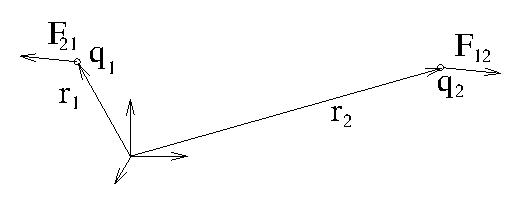
\includegraphics[scale=1]{immagini/fisica2/forza_coulomb}
\end{figure}
La \eqref{coulomb01} la possiamo riscrivere usando la \eqref{norm02}:
\[\ve{F}_{12}=K_e\frac{q_1q_2}{r_{12}^3}\ve{r_{12}}\]
oppure se $\ve r_1$ individua $q_1$ rispetto all'origine e $\ve r_2$ $q_2$:
\[
\ve{F}_{12}=K_e\frac{q_1q_2}{\norm{\ve r_2-\ve r_1}^3}\left(\ve r_2-\ve r_1\right)
\]
Naturalmente per la terza legge della dinamica:
\[
\ve F_{12}=-\ve F_{21}
\]
\subsection{Unità di misura}
Un'idea è quella di porre $K_e=1$ e di definire la carica unitaria quella carica che posta alla distanza unitaria da una carica unitaria produce una forza unitaria. Questo è quello che si fa nel sistema CGS Elettrostatico\index{CGS elettrostatico}. Non si definisce a priori la carica, che prende il nome di u.e.s.\@ unità elettrostatica semplice\index{unità elettrostatica semplice}, chiamata anche stat--coulomb\index{stat--coulomb}.

Il secondo modo è di definire a priori la carica, ed è quello che si fa nel Sistema Internazionale. Si definisce coulomb\index{coulomb} quella carica che attraversando un voltametro al nitrato d'argento ($\mathrm{AgNO_3}$) deposita sul catodo una quantità di Ag di \si{0.00111800}{\gram}. \`E una definizione provvisoria. Si ricava quindi $K_e\simeq \si{8.8974E9}{\newton\meter\squared\per\coulomb\squared}$. Nell'ambito del SI si è comodo usare il sistema razionalizzato Giorgi\index{Giorgi}\index{sistema!razionalizzato Giorgi}, nella quale $K_e=\frac{1}{4\pi\varepsilon_0}$, $\varepsilon_0\simeq \si{8.8E-12}{\coulomb\squared\per\newton\metre\squared}$.

Il coulomb e lo stat-coulomb nonostante siano unità della stessa grandezza hanno dimensioni diverse.
\begin{Es}[pendolo magnetico]
\begin{figure}[htbp]
\centering
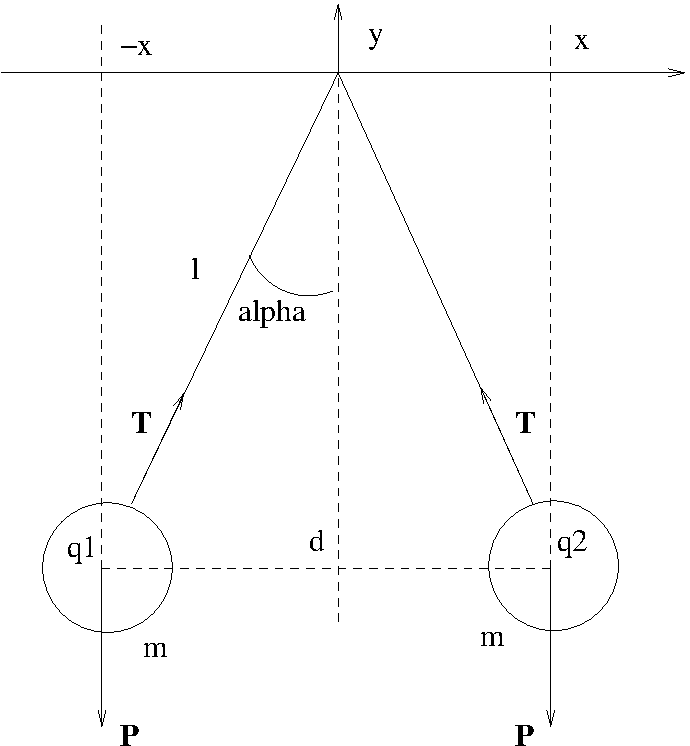
\includegraphics[scale=0.5]{immagini/fisica2/pendolo_carico}
\end{figure}
\end{Es}
Ci si chiede l'equilibrio del pendolo in figura. Se $q_1q_2<0$ allora l'equilibrio è $x=0$.
\[\ve F_e=\frac{q_1q_2}{4\pi\varepsilon_0}\frac{1}{d^2}\ver e_{q_1,q_2}=\frac{q_1q_2}{4\pi\varepsilon_0}\frac{1}{4x^2}\ver x\]
\[\ve P=-mg\ver \jmath\]
Scomponendo sugli assi e imponendo l'equilibrio:
\[\left\{\begin{array}{l}
T\sin\alpha\ver \imath-\dfrac{q_1q_2}{4\pi\varepsilon_0}\dfrac{1}{4x^2}\ver \imath=0\\
T\cos\alpha\ver \jmath-mg\ver \jmath=0
\end{array}\right.\]
Dividendo e usando $x=l\sin\alpha$
\[\tan\alpha=\frac{q_1q_2}{16\pi\varepsilon_0mgl^2}\frac{1}{\sin^2\alpha}\]
\[\sin^2\alpha=1-\frac{1}{1+\tan^2\alpha}\qquad\frac{1}{\sin^2\alpha}=\frac{1+\tan^2\alpha}{\tan^2\alpha}\]
\[\tan^3\alpha=\frac{q_1q_2}{16\pi\varepsilon_0mgl^2}(1+\tan^2\alpha)\]
Ipotizziamo che $\alpha\ll 1$, allora $\tan\alpha\simeq\alpha$:
\[\alpha=\sqrt[3]{\frac{q_1q_2}{16\pi\varepsilon_0mgl^2}}\]
Naturalmente se $y_1\neq y_2$ allora le soluzioni potrebbero essere altre. Se scostiamo di poco una massa dalla posizione di equilibrio $x_0=l\alpha$ di $\delta_x=(x-x_0)$ la forza (primo sviluppo di Taylor) risulta:
\[F(x)=F(x_0-\delta_x)=F(x_0)+F'(x_0)\delta_x=F'(x_0)\delta_x\]
l'equazione del moto diventa:
\[m\ddot x=F'(x_0)\delta_x\]


\section{Densità di carica\index{densità di carica}}
Al posto di immaginare la materia come un discreto con cariche puntiformi possiamo immaginarla, a livello macroscopico, come un continuo, definendo una densità di carica volumetrica. Sia $V$ un volume, e $\Delta V$ una porzione di essa. All'interno di $\Delta V$ è contenuta la carica $\Delta q$. Definiamo densità volumetrica di carica la funzione\index{densità di carica!volumetrica}:
\[\rho\left({\ve r}\right)=\lim_{\Delta V\to 0}\frac{\Delta q}{\Delta V}=\frac{\ud q}{\ud V}\]
La carica totale è allora:
\[Q=\int_V\rho(\ve r)\,\ud V\]
Allo stesso modo possiamo definire una densità superficiale di carica \index{densità di carica!superficiale}$\sigma(\ve r)$, o lineare \index{densità di carica!lineare}$\lambda(\ve r)$.
\subsection{Forza}
La forza dell'elementino $\ud V$ sulla carica puntiforme esterna $q$ è 
\[\ud\ve F=\frac{1}{4\pi\varepsilon_0}\frac{q\,\ud q}{\norm{\ve r-{\ve r}\,^\prime}^3}\left(\ve r-{\ve r}\,^\prime\right)\]
\[\ve F=\int_V \ud \ve F=\frac{q}{4\pi\varepsilon_0}\int_V\frac{\
\rho(\ve r\,^\prime)\left(\ve r-{\ve r}\,^\prime\right)}{\norm{\ve r-{\ve r}\,^\prime}^3}\,\ud V\]
\section{Campo elettrico\index{campo!elettrico}\index{campo!elettrostatico}}
Fino ad ora abbiamo usato il concetto di azione a distanza\index{azione a distanza},
%\[{\oint\limits_0^1}_{\Gamma}\]
%\[\mathop{{\int\!\!\!\!\!\int}\mkern-21mu \bigcirc}\limits_{3}{{\mathop{\rm{x}}}}\]
%\[\mathop{{\int\!\!\!\!\!\int\!\!\!\!\!\int}\mkern-31.2mu\bigodot}\limits_{0}{{\mathop{\rm x}}}}\]
cioè una carica produce direttamente (o attraverso le linee di forza) una forza su un'altra carica. L'altro modo di pensare è che una carica modifica il campo elettrostatico, il quale produce una forza su un'altra carica. Definiamo il campo elettrostatico:
\[\ve E=\frac{\ve F}{q}\]
con $\ve F$ la forza esercitata dalla carica generante il campo sulla carica esplorativa e $q$ il valore della carica esplorativa, cioè la carica su cui agisce il campo. Può essere interpretato come la forza nell'unità di carica. Per una carica puntiforme $q$ nell'origine abbiamo:
\begin{equation}
\ve E=\frac{1}{4\pi\varepsilon_0}\frac{q}{{\norm{\ve r}}^3}\ve r
\end{equation}
\subsection{Definizione operativa\index{campo!elettrostatico}}
Abbiamo definito il campo elettrostatico come la forza sulla carica di prova: è una definizione puramente matematica. Il problema dal punto di vista operativo è che se vogliamo misurare un campo elettrostatico con una carica di prova, questa modificherà la distribuzione di cariche generatrici del campo e quindi usando cariche di prova diverse troveremo campi leggermente diversi. Bisogna allora usare cariche di prova più piccole possibili, in teoria tendenti a zero. In realtà il campo non dipende dalla carica di prova, è una proprietà fisica dello spazio, ma per misurarlo abbiamo bisogno di una carica di prova. Si potrebbe definire il campo elettrostatico come $\ve E=\lim_{q\to 0}\frac{\ve F}{q}$.
\begin{Es}[campo elettrico di una distribuzione lineare]
\begin{figure}[htbp]
\centering
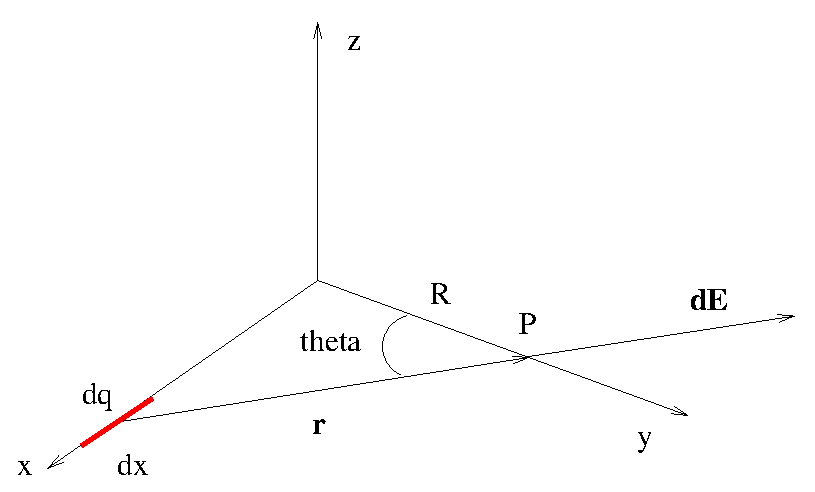
\includegraphics[scale=0.6]{immagini/fisica2/filo_inf}
\end{figure}
Im\-ma\-gi\-nia\-mo un filo infinito in coincidenza dell'asse $x$ sul quale sia depositata una densità lineare $\lambda$ uniforme. Il fatto che il filo sia di lunghezza infinita semplifica notevolmente i conti per motivi di simmetria, infatti possiamo dire in qualunque punto lungo l'asse $y$ ci mettiamo di avere metà filo a destra e metà a sinistra. Sia $P$ un punto sull'asse $y$: $P=(0,R,0)$. Consideriamo un elementino del filo $\ud x$, esisterà un altro elementino simmetrico che annulla la componente $x$ del campo; questo per ogni porzione del filo si consideri, in quanto infinito. L'elementino $\ud x$ genera in $P$ un campo $\ud \ve E$. La carica su $\ud x$ è $\ud q=\ud x\lambda$, quindi:
\[\ud\ve E=\frac{1}{4\pi\varepsilon_0}\frac{\lambda\ud x}{r^3}\ve r\]
\[\ud E_y=\frac{1}{4\pi\varepsilon_0}\frac{\lambda\ud x}{r^3}r\cos\theta\quad \ud E_x=\ud E_z=0\]
\[x=R\tan\theta\quad\ud x=R\frac{1}{\cos^2\theta}\ud\theta\quad r=\frac{R}{\cos\theta}\]
\begin{align*}E_y&=\int\ud E_y=\int_{-\infty}^{+\infty}\frac{1}{4\pi\varepsilon_0}\frac{\lambda\ud x}{r^2}\cos\theta=\frac{\lambda}{4\pi\varepsilon_0}\int_{-\infty}^{+\infty}\frac{\ud x}{r^2}\cos\theta\\
&=\frac{\lambda}{4\pi\varepsilon_0}\frac{1}{R}\int_{-\frac{\pi}{2}}^{+\frac{\pi}{2}}\cos\theta\ud\theta=\frac{1}{4\pi\varepsilon_0}\frac{2\lambda}{R}
\end{align*}
\[\ve E=\frac{1}{4\pi\varepsilon_0}\frac{2\lambda}{R}\ver{j}\]
L'ipotesi del filo infinito fisicamente può essere interpretato come $R\ll l$ con $l$ la lunghezza del filo.
\end{Es}
\begin{Es}[Anello]
\label{es:anello}
Vogliamo calcolare il valore di $\ve E$ lungo l'asse di un anello con carica totale $q$ uniforme.
\begin{figure}[htbp]
\centering
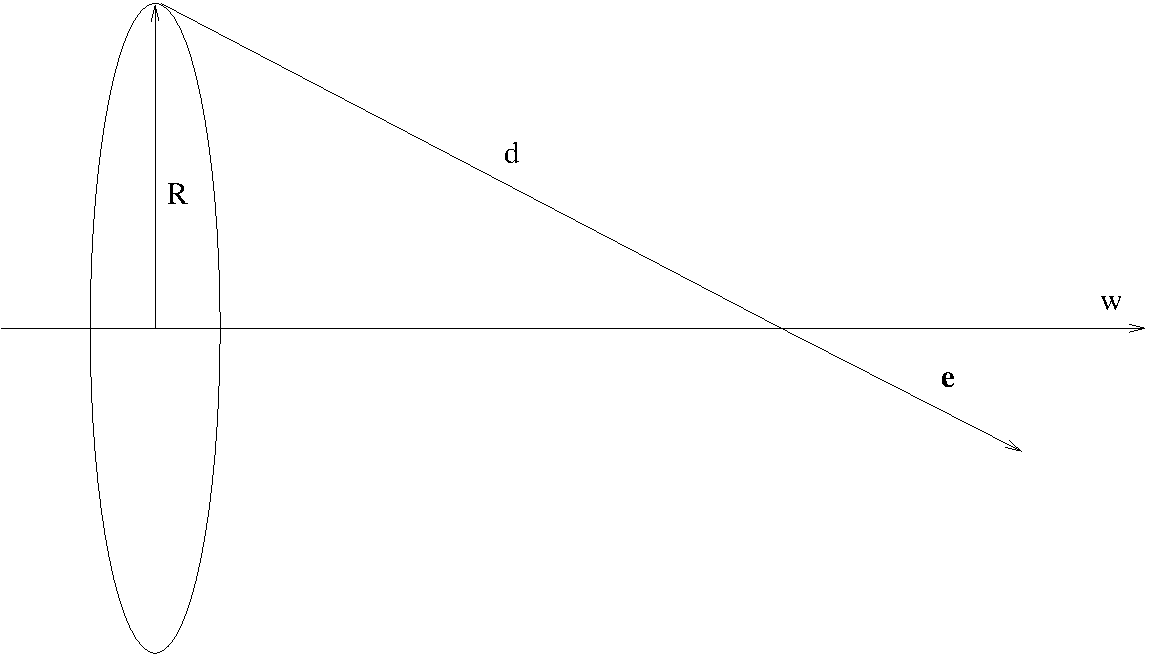
\includegraphics[scale=0.45]{immagini/fisica2/anello}
\end{figure}
Data la simmetria del problema usiamo coordinate cilindriche. Per ragioni di simmetria il campo sarà rivolto come il versore $\ver e_w$. Ricaviamo il versore $\ver e$:
\[\ver e=\cos\alpha\ver e_w+\sin\alpha\ver e_r=\frac{w}{d}\ver e_w+\frac{R}{d}\ver e_r\]
Sull'elementino infinitesimo dell'anello è depositata la carica $\ud q=\frac{q \ud \theta}{2\pi}$ e $d^2=w^2+R^2$:
\begin{align*}
\ve E(0,0,w)&=\int_C\frac{\ud q}{4\pi\varepsilon_0d^2}\ver e\\
&=\int_0^{2\pi}\frac{q}{2\pi}\frac{\ud\theta}{4\pi\varepsilon_0}\frac{1}{R^2+w^2}\ver e\\
&=\int_0^{2\pi}\frac{q}{2\pi}\frac{\ud\theta}{4\pi\varepsilon_0}\frac{1}{R^2+w^2}\left[\frac{w}{\sqrt{R^2+w^2}}\ver e_w+\frac{R}{\sqrt{R^2+w^2}}\ver e_r\right]\\
&=\frac{q}{2\pi}\frac{\ud\theta}{4\pi\varepsilon_0}\frac{1}{R^2+w^2}\left[\frac{w}{\sqrt{R^2+w^2}}\ver e_w\right]\int_0^{2\pi}\ud\theta\\
&=\frac{q}{4\pi\varepsilon_0}\frac{w}{(R^2+w^2)^{\frac{3}{2}}}\ver e_w\\
\end{align*}
Se $w\to +\infty$ coerentemente:
\[\ve E(0,0,w)\to\frac{q}{4\pi\varepsilon_0}\frac{\ver e_w}{w^2}\]
cioè come un punto.
\end{Es}
\begin{Es}[Disco]
\begin{figure}[htbp]
 \centering
 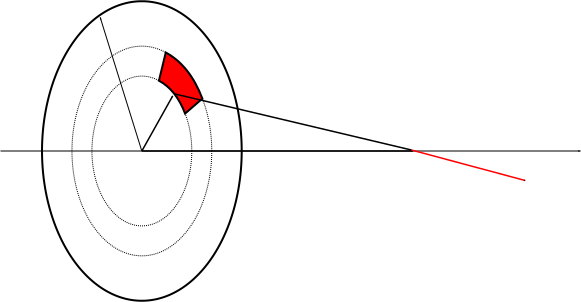
\includegraphics[scale=0.8]{immagini/fisica2/disco}
\end{figure}
 Consideriamo un disco di raggio $R$ e carica superficiale uniforme $\sigma$. Calcoliamo il campo elettrostatico sull'asse del disco $z$ nel punto $\ve r$. La carica di un elementino infinitesimo sarà:
\[
 \ud q' = \sigma\ud a = \sigma r'\ud\varphi'\ud r'
\]
Il campo che genera sarà:
\[
 \ud\ve E = \frac{1}{4\pi\varepsilon_0}\ud q'\frac{\ve r-\ve r'}{\norm{\ve r-\ve r'}^3}
\]
calcoliamo $\ve r-\ve r'$:
\begin{gather*}
 \ve r-\ve r'=-r' \ver e_r + z\ver k\\
 \norm{\ve r-\ve r'} = (r'^2+z^2)^{1/2}
\end{gather*}
\begin{align*}
 \ve E(0,0,z) &= \frac{1}{4\pi\varepsilon_0}\int \ud q'\frac{\ve r-\ve r'}{\norm{\ve r-\ve r}^3}\\
 &=\frac{1}{4\pi\varepsilon_0}\int \sigma r'\ud r'\ud\varphi'\frac{-r'\ver e_r+z\ver k}{(r'^2+z^2)^{3/2}}\\
 &=\frac{\sigma}{4\pi\varepsilon_0}\int\ud r'\int\ud\varphi\frac{-r'^2\ver e_r+r' z\ver k}{(r'^2+z^2)^{3/2}}\\
 &=\frac{\sigma}{4\pi\varepsilon_0}\int_0^R \ud r'\frac{zr'\ver k}{(r'^2+z^2)^{3/2}}\int_0^{2\pi}\ud\varphi'\\
 &=\frac{\sigma}{4\pi\varepsilon_0}2\pi z\ver k\int_0^R\frac{r'\ud r'}{(r'^2+z^2)^{3/2}}
\end{align*}
questo risultato si può trovare usando l'esempio precedente \ref{es:anello}, in cui $\ve E = \frac{\lambda 2\pi r'}{4\pi\varepsilon_0}\frac{z}{(R^2+z^2)^{3/2}}\ver k$ e $\sigma\ud r=\lambda$, in quando deve essere $\ud q = \sigma\ud a=\lambda r \ud \varphi$. Usando la sostituzione $s = r'^2+z^2$, $\ud s = 2r'\ud r$:
\begin{align*}
 \ve E(0,0,z) &=\frac{\sigma}{4\pi\varepsilon_0}2\pi z\ver k\int_{z^2}^{R^2+z^2}\frac{\ud s}{2s^{3/2}}\\
 &=\frac{\sigma}{4\pi\varepsilon_0}2\pi z\ver k\left.\frac{-2}{2s^{1/2}}\right|_{z^2}^{R^2+z^2}\\
 &=\frac{\sigma}{4\pi\varepsilon_0}2\pi z\ver k\left(\frac{-1}{\sqrt{R^2+z^2}}-\frac{-1}{\sqrt{z^2}}\right)\\
 &=\frac{\sigma}{2\varepsilon_0} z\left(\frac{1}{|z|}-\frac{1}{\sqrt{R^2+z^2}}\right)\ver k
\end{align*}
\begin{figure}[htbp]
 \centering
 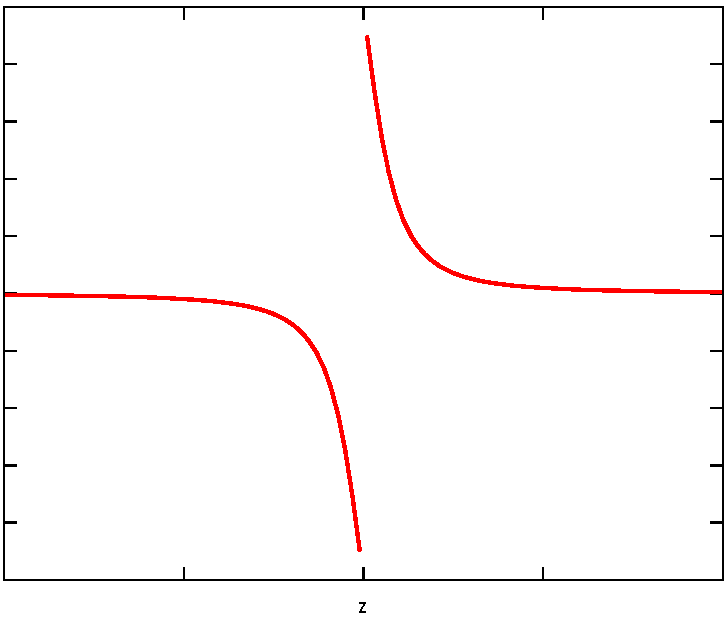
\includegraphics[scale=0.5]{immagini/fisica2/potenziale_disco}
 \caption{Campo elettrico del disco lungo $z$.}
\end{figure}

Se sono molto vicino al disco:
\[
 \lim_{z\to 0^\pm}\ve E(0,0,z)=\lim_{z\to 0^\pm} \frac{\sigma}{2\varepsilon_0} z\left(\frac{1}{|z|}-\frac{1}{\sqrt{R^2+z^2}}\right)\ver k=\pm\frac{\sigma}{2\varepsilon_0}\ver k
\]
\end{Es}
\begin{Es}[filo finito]
 Consideriamo un filo di lunghezza finita sull'asse $z$ con densità di carica uniforme $\lambda$. Vogliamo trovare il campo elettrostatico lungo l'asse $x$. Un elementino infinitesimo avrà carica $\ud q'=\lambda\ud z'$. e genererà un campo:
\[
 \ud\ve E(x,0,0) = \frac{\ud q'}{4\pi\varepsilon_0}\frac{\ve r-\ve r'}{\norm{\ve r-\ve r'}^3}
\]
con $\ve r=x\ver i$, $\ve r'=z\ver k$, $\ve r-\ve r'=x\ver i-z \ver k$
\[
 \ve E(x,0,0)=\int\ud \ve E=\frac{\lambda}{4\pi\varepsilon_0}\int\frac{x\ver i-z\ver k}{(x^2+z'^2)^{3/2}}\ud z'
\]
per risolvere l'integrale è utile la sostituzione $\tan\gamma=\frac{z'}{x}$:
\begin{align*}
 \ve E(x,0,0)&=\frac{\lambda}{4\pi\varepsilon_0}\int\frac{x(1+\tan^2\gamma)\ud\gamma}{x^3\left(1+\tan^2\gamma\right)^{3/2}}\left(x\ver i-x\tan\gamma\ver k\right)\\
&=\frac{\lambda}{4\pi\varepsilon_0}\frac{1}{x}\int\frac{\ver i-\tan\gamma\ver k}{\left(1+\tan^2\gamma\right)^{1/2}}\\
&=\frac{\lambda}{4\pi\varepsilon_0}\frac{1}{x}\int\left(\cos\gamma\ver i-\sin\gamma\ver k\right)
\end{align*}
se $z$ varia tra $(z_\text{min},z_\text{max})$, $\gamma$ varia tra $(\gamma_\text{min},\gamma_\text{max})=\arctan\left(\frac{z_\text{max}}{x},\frac{z_\text{min}}{x}\right)$:
\begin{align*}
 \ve E(x,0,0)&=\frac{\lambda}{4\pi\varepsilon_0}\frac{1}{x}\int_{\gamma_{\text{min}}}^{\gamma_{\text{max}}}\ud\gamma\left(\cos\gamma\ver i-\sin\gamma\ver k\right)\\
&=\frac{\lambda}{4\pi\varepsilon_0}\frac{1}{x}\left[\left(\sin\gamma_\text{max}-\sin\gamma_\text{min}\right)\ver i+\left(\cos\gamma_\text{max}-\cos\gamma_\text{min}\right)\ver k\right]
\end{align*}



\end{Es}


\section{Teorema di Gauss\index{Gauss}\index{teorema!di Gauss}}
\label{teorema_di_gauss}
Immaginiamo una carica puntiforme contenuta in una superficie immaginaria $S$. Per definizione il flusso attraverso $S$ è 
\begin{equation}
\Phi_S(\ve E)=\oint_S\ve E\cdot\ve n\,\ud a
\label{gauss01}
\end{equation}
Sostituendo nella \eqref{gauss01} il campo elettrico di una carica puntiforme $\ve E=\frac{q}{4\pi\varepsilon_0}\frac{\ve r}{r^3}$ si ottiene:
\begin{align*}
\Phi_S(\ve E)&=\frac{q}{4\pi\varepsilon_0}\oint_S\frac{\ve r\cdot\ve n}{r^3}\ud a=\frac{q}{4\pi\varepsilon_0}\oint_S\frac{r\cos\theta}{r^3}\ud a\\
&=\frac{q}{4\pi\varepsilon_0}\oint_S\frac{\ud a_0}{r^2}=\frac{q}{4\pi\varepsilon_0}\oint_S\ud\omega=\frac{q}{4\pi\varepsilon_0}4\pi=\frac{q}{\varepsilon_0}
\end{align*}
Infatti $\ud a\cos\theta=\ud a_0$ cioè l'elementino di area infinitesima orientato perpendicolarmente a $\ve E$, mentre $\ud \omega=\frac{\ud a_0}{r^2}$ è per definizione l'angolo solido infinitesimo che sotteso dall'area infinitesima $\ud a_0$.

Questo importante risultato è indipendente dalla geometria della superficie, infatti l'integrale dell'angolo solido su qualsiasi superficie considerata nella sua interezza è $4\pi$ (qui si nota la comodità del sistema razionalizzato). Il risultato poi è valido per qualsiasi forza del tipo $\frac{1}{r^2}$ infatti mentre l'area aumenta col quadrato della distanza, il campo diminuisce col quadrato della distanza e le due cose si semplificano a vicenda.

Se la carica fosse sul bordo della superficie, l'integrale dell'angolo solido sarebbe stato $2\pi$ e quindi:
\[\Phi_S(\ve E)=\frac{1}{2}\frac{q}{\varepsilon_0}\]

Se la carica fosse stata presa all'esterno della superficie allora il flusso attraverso essa sarebbe stato nullo (da una parte entra, dall'altra esce in egual misura), infatti considerando un areola infinitesima $\ud a_1$ o meglio la sua componente normale al campo $\ud a_{01}$ ne corrisponde una $\ud a_{02}$ dove il flusso è uscente. Il flusso netto attraverso queste due superfici è \[\ud\Phi_S(\ve E)=\frac{q}{4\pi\varepsilon_0}\left(\ud\omega_1-\ud\omega_2\right)=0\]
perché $\ud\omega_1=\ud\omega_2$ e perché naturalmente ad ogni areola in cui il campo entra corrisponde una ed una sola areola in cui il campo esce.

Se mettiamo più di una carica puntiforme usiamo il principio di sovrapposizione sul campo, e quindi sul flusso:
\[\ve E=\sum_{i=1}^n \ve E_i\Rightarrow \Phi_S(\ve E)=\oint_S\left(\sum_{i=1}^n\ve E\right)\ve n\,\ud a\]
\begin{Teo}[Gauss per cariche puntiformi]
Sia $S$ una superficie chiusa e $\{q_i\}_{i=1}^n$ cariche interne ad $S$, definiamo $Q=\sum_{i=1}^n q_i$ allora:
\begin{equation}
\Phi_S(\ve E)=\frac{Q}{\varepsilon_0}
\end{equation}
\end{Teo}
Per una distribuzione di cariche nello spazio $\rho(\ve r)$ basta ricordare che $Q=\int_V\rho(\ve r)\ud v$, quindi:
\begin{Teo}[Gauss]
Sia $S$ una superficie chiusa, al suo interno vi sia una distribuzione continua di carica $\rho(\ve r)$, allora:
\begin{equation}
\Phi_S(\ve E)=\frac{1}{\varepsilon_0}\int_V\rho\,\ud v
\end{equation}
\end{Teo}
Usando il teorema della divergenza:
\[\Phi_S(\ve E)=\int_S\ve E\cdot\ve n\,\ud a=\int_V\diver\ve E\,\ud v=\frac{1}{\varepsilon_0}\int_V\rho\,\ud v\]
Allora dato che l'integrale vale per qualsiasi superficie e quindi volume, abbiamo:
\begin{equation}
\diver \ve E(\ve r)=\frac{\rho(\ve r)}{\varepsilon_0}
\end{equation}
che esprime il teorema di Gauss in forma differenziale. Riassumendo:
\begin{equation}
\ve\nabla\cdot\ve E(\ve r)=\frac{\rho(\ve r)}{\varepsilon_0}\qquad \forall S\,\int_S \ve E\cdot\ve n\,\ud a=\frac{Q}{\varepsilon_0}
\end{equation}
con $Q$ le cariche interne ad $S$.
\begin{Es}[campo sfera piena]
Sia $B$ una sfera piena di raggio $R$ centrata nell'origine, con densità di carica $\rho$ uniforme. Vogliamo il campo elettrico. Data la simmetria usiamo coordinate sferiche. Dobbiamo dividere lo spazio in due semispazi, uno con $r<R$ e l'altro con $r>R$.
\[\ve E(r,\theta,\varphi)=E_r\ver e_r+E_\theta\ver e_\theta+E_\varphi \ver e_\varphi=E_r(r)\ver e_r\]
infatti il campo è radiale e dipende solo dalla distanza dal centro per ragioni di simmetria per rotazioni.
All'esterno, $r>R$, allora prendiamo una superficie $S$ sferica passante per $P$:
\[\Phi_S(\ve E)=\oint_S\ve E\cdot\ve n\,\ud a=\oint_S E\ud a=E\oint_S \ud a=4\pi r^2 E\]
Per il teorema di Gauss:
\[\Phi_S(\ve E)=\frac{Q}{\varepsilon_0}=\frac{\frac{4}{3}\pi R^3\rho}{\varepsilon_0}\]
confrontando:
\[\ve E(\ve r)=\frac{\rho}{3\varepsilon_0}\frac{R^3}{r^2}\ver e_r=\frac{Q^{\text{tot}}}{4\pi\varepsilon_0}\frac{1}{r^2}\ver e_r\]
Esattamente come se tutta la carica fosse concentrata al centro. All'interno $r<R$, prendiamo una superficie gaussiana $S$ passante per $P$:
\[\Phi_S(\ve E)=\oint_S\ve E\cdot\ve n\,\ud a=\oint_S E\ud a=E\oint_S \ud a=4\pi r^2 E\]
Questa volta le cariche contenute nella superficie gaussiana non sono tutte le cariche:
\[\Phi_S(\ve E)=\frac{Q}{\varepsilon_0}=\frac{\frac{4}{3}\pi r^3\rho}{\varepsilon_0}\]
confrontando:
\[\ve E(\ve r)=\frac{\rho}{3\varepsilon_0}r\ve e_r\]
Il massimo si ha quando $\norm{\ve r}=R$. La funzione che descrive il campo è continua (basta verificarlo per $r=R$), ma ha un punto angoloso.
\begin{figure}[htbp]
\centering
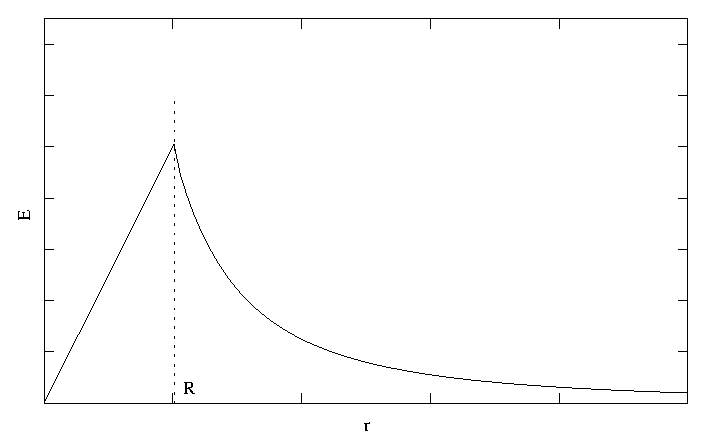
\includegraphics{immagini/fisica2/campo_sfera}
\caption{Campo di una sfera piena uniformemente carica.}
\end{figure}
\end{Es}
\begin{Es}[Piano]
Consideriamo un piano uniformemente carico con distribuzione $\sigma$. Per ragioni di simmetria il campo è perpendicolare al piano. Costruiamo una superficie gaussiana a forma di parallelepipedo, in modo che intersechi il piano. Il flusso non è nullo solo sulle facce parallele al piano. Usando Gauss:
\begin{align*}
\Phi_S(\ve E)=&\Phi_{S_1}(\ve E)+\Phi_{S_2}(\ve E)=\int_{S_1}\ve E\cdot\ve n\,\ud a+\int_{S_2}\ve E\cdot\ve n\,\ud a=2EA\\
=&\frac{Q}{\varepsilon_0}=\frac{1}{\varepsilon_0}\int_A \sigma\,\ud a=\frac{\sigma A}{\varepsilon_0}
\end{align*}
Allora:
\[E=\frac{\sigma}{2\varepsilon_0}\]
Notare che non dipende dalla distanza.
\end{Es}
\begin{Es}[condensatore piano\index{condensatore!piano}]
Consideriamo due lastre molto vicine, che equivale a dire due lastre infinite, parallele con distribuzione $\pm\sigma$. Usando il risultato dell'esempio precedente e del principio di sovrapposizione, ricordando che stiamo sommando quantità vettoriali, possiamo dire che il campo all'esterno è nullo ovunque, mentre tra le due armature è doppio:
\[E=\frac{\sigma}{\varepsilon_0}\]
diretto dall'armatura positiva a quella negativa.
\end{Es}
\section{Potenziale elettrostatico\index{potenziale!elettrostatico}}
\begin{figure}[htp]
 \centering
 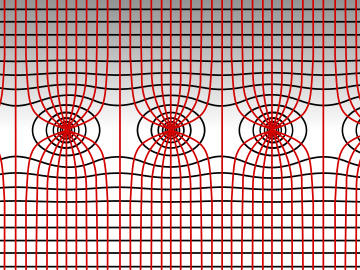
\includegraphics{immagini/fisica2/MWPC}
 \caption{Linee equipotenziali (in nero) e linee di campo (in rosso) per una camera proporzionale a multifili (anodi al centro e catodi sopra e sotto).}
\end{figure}
\begin{Def}[differenza di potenziale]
La differenza di potenziale tra $P_1$ e $P_2$ è il lavoro svolto per spostare una carica unitaria contro le forze del campo elettrostatico tra i due punti:
\begin{equation}
 \Delta\varphi=\varphi(P_2)-\varphi(P_1)=\frac{L_{P_1}^{P_2}}{q} 
\end{equation}
\end{Def}
\begin{figure}[htp]
 \centering
 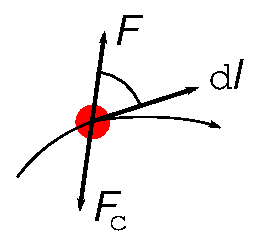
\includegraphics{immagini/fisica2/lavoro_campo}
\end{figure}

Consideriamo un campo $\ve E(\ve r)$ e una carica $q_0$ che si muove su una curva $\Gamma$ congiungente $P_1$ e $P_2$. Dividiamo $\Gamma$ in infinitesimi pezzi $\ud\ve l$, il lavoro elementare compiuto dal campo è 
\[\delta L_c=\ve F_c\cdot\ud\ve l\]
Il lavoro totale compiuto dal campo è l'integrale di tutti i lavori elementari:
\[L_c=\int_{P_1}^{P_2}\ve F_c\cdot\ud\ve l=\int_{P_1}^{P_2}q_0\ve E(\ve r)\cdot \ud \ve l\]
Allora noi dovremo svolgere un lavoro $L=-L_c$ perché la nostra forza $\ve F=-\ve F_c$, dunque:
\[\frac{L}{q_0}=-\int_{P_1}^{P_2}\frac{\ve F_c\cdot\ud\ve l}{q_0}=-\int_{P_1}^{P_2}\ve E(\ve r)\cdot\ud\ve l\]
Questa è la differenza di potenziale tra $P_1$ e $P_2$ se si dimostra che non dipende dal cammino, cioè da $\Gamma$.

Consideriamo il campo generato da una carica puntiforme nell'origine, allora per andare da $P_1$ a $P_2$:
\begin{align*}
\frac{L}{q}&=-\int_{P_1}^{P_2}\ve E\cdot\ud\ve l=-\int_{P_1}^{P_2}\frac{q}{4\pi\varepsilon_0}\frac{\ve r\cdot\ud\ve l}{r^3}=-\frac{q}{4\pi\varepsilon_0}\int_{P_1}^{P_2}\frac{\cos\theta\,\ud l}{r^2}\\
&=-\frac{q}{4\pi\varepsilon_0}\int_{r_1}^{r_2}\frac{\ud r}{r^2}=\frac{q}{4\pi\varepsilon_0}\left(\frac{1}{r_2}-\frac{1}{r_1}\right)
\end{align*}
Dunque non dipende dal cammino percorso e possiamo dire che:
\begin{Teo}[differenza di potenziale]
\begin{equation}
\Delta \varphi=-\int_{P_1}^{P_2}\ve E(\ve r)\cdot\ud\ve l=\varphi(P_2)-\varphi(P_1)
\end{equation}
\end{Teo}
Possiamo prendere un riferimento $P_0$ e dire che $\varphi(P_0)=k$, allora $\varphi(P_1)$ sarà il lavoro per portare la carica da $P_0$ a $P_1$ e sarà la differenza di potenziale tra $P_0$ e $P_1$; $\varphi(P_2)$ la differenza di potenziale tra $P_0$ e $P_2$. Allora:
\[\Delta \varphi=-\int_{P_1}^{P_2}\ve E\cdot\ud\ve l=-\int_{P_1}^{P_0}\ve E\cdot\ud\ve l-\int_{P_0}^{P_2}\ve E\cdot\ud\ve l=\varphi(P_0)-\varphi(P_1)+\varphi(P_2)-\varphi(P_0)\]
Dunque è indipendente dalla scelta di $P_0$. Per convenzione\footnote{un'altra convenzione è mettere il potenziale della Terra uguale a zero, vedi \eqref{potenziale_terra} a pag.\@\pageref{potenziale_terra}}:
\[\varphi(\infty)=0\]
Quindi per portare una carica dall'infinito:
\[\frac{L}{q_0}=-\int_{\infty}^{P}\ve E\cdot\ud \ve l=\varphi(P)\]
Definiamo il potenziale in un punto (avendo preso come riferimento l'infinito):
\begin{Def}[potenziale]
\begin{equation}
\varphi(P)=-\int_{\infty}^P\ve E(\ve r)\cdot\ud\ve l
\end{equation}
il lavoro che devo fare per portare la carica unitaria dall'infinito al punto contro le forze del campo.
\end{Def}
\begin{Es}[carica puntiforme nell'origine]
\[
\varphi(\ve r)=-\int_{\infty}^r\frac{q}{4\pi\varepsilon_0}\frac{\ve r\cdot\ud\ve l}{r^3}=-\frac{q}{4\pi\varepsilon_0}\int_\infty^r\frac{r}{r^3}\ud r=\frac{q}{4\pi\varepsilon_0}\frac{1}{r}
\]
\end{Es}
\subsection{Potenziale di qualsiasi distribuzione}
L'espressione del potenziale può essere ricavata notando che $\ve\nabla\frac{1}{r}=-\frac{\ve r}{r^3}$:
\begin{equation}
\begin{split}
 \ve E &= \frac{1}{\giorgi}\int_V \rho(\ve r')\frac{\ve r-\ve r'}{\norm{\ve r-\ve r'}^3}\,\ud V'\\
&=-\frac{1}{\giorgi}\int_V \rho(\ve r')\ve\nabla\left(\frac{1}{\ve r-\ve r'}\right)\,\ud V'\\
&=-\ve\nabla\int_V \frac{1}{\giorgi}\frac{\rho(\ve r')}{\ve r-\ve r'}\,\ud V'\\
&=-\ve\nabla\varphi(\ve r)
\end{split}
\end{equation}
per vedere che questo $\varphi$ è proprio il potenziale di prima
\[
\grad \varphi\cdot\ud\ve l=\ud \varphi=\frac{\delta L}{q}=-\ve E\cdot\ud \ve l\Rightarrow \ve E=-\grad\varphi
\]
In generale, considerando anche cariche puntiformi e superficiali:
\begin{equation}\varphi(\ve r)=\frac{1}{4\pi\varepsilon_0}\left[\sum_i\frac{q_i}{\norm{\ve r-\ve r_i}}+\int_S\frac{\sigma({\ve r}\,')}{\norm{\ve r-\ve r\,'}}\ud a+\int_V\frac{\rho({\ve r}\,')}{\norm{\ve r-{\ve r}\,'}}\ud V\right]\end{equation}
\section{Energia potenziale\index{energia!potenziale!elettrostatica}}
Il potenziale è indipendente dalla carica di prova, l'energia potenziale no. \`E la stessa differenza che c'è tra la forza elettrostatica e il campo elettrostatico, quindi:
\[\Delta W=q\Delta \varphi\]
Rifacendo il discorso per il potenziale: siano $A$ e $B$ due punti, l'integrale è indipendente dal percorso quindi:
\[L_A^B=\int_A^B \ve F\cdot\ud\ve l=-q\int_A^B\ve E\cdot\ud\ve l=q\Delta \varphi=\Delta W=W_B-W_A\]
Per il calcolo abbiamo usato la forza contro le forze del campo, non la forza del campo. Il lavoro a sinistra il lavoro contro le forze del campo, mentre l'energia potenziale a destra è relativa alle forze del campo: ecco perché non c'è il meno.
\subsection{Unità di misura}
Nel SI il potenziale si misura in volt\index{volt}:
\[[\varphi]=\frac{\joule}{\coulomb}=\volt\]
allora essendo $\ve E=-\ve\nabla\varphi$ il campo lo possiamo esprimere in:
\[[\ve E]=[-\ve\nabla\varphi]=\frac{\volt}{\metre}\]
\[[U]=\joule=[q\varphi]=\coulomb\volt\]
\subsection{Energia di un sistema di cariche\index{energia!di un sistema di cariche}}
Prendiamo una carica $q_1$, portiamola dall'infinito alla posizione $\ve r_1$: non serve compiere lavoro. Ora abbiamo un campo, con un potenziale $\varphi_1(\ve r)$. Prendiamo un'altra carica $q_2$ e portiamola dall'infinito alla posizione $\ve r_2$: dobbiamo compiere un lavoro contro le forze del campo:
\[L_\infty^{\ve r_2}=\int_\infty^{\ve r_2}\ve F\cdot\ud \ve l=-q_2\int_\infty^{\ve r_2} \ve E\cdot\ud \ve l=q_2\varphi_1(\ve r_2)\]
Aggiungiamo una carica $q_3$ in posizione $\ve r_3$, altro lavoro:
\[L_\infty^{\ve r_3}=q_3\varphi_1(\ve r_3)+q_3\varphi_2(\ve r_3)\]
Il lavoro che compiamo va ad accrescere l'energia potenziale del sistema $W$, a questo punto:
\begin{align*}
W&=q_2\varphi_1(\ve r_2)+q_3\varphi_1(\ve r_3)+q_3\varphi_2(\ve r_3)\\
&=\frac{q_1q_2}{4\pi\varepsilon_0}\frac{1}{\norm{\ve r_1-\ve r_2}}+\frac{q_1q_3}{4\pi\varepsilon_0}\frac{1}{\norm{\ve r_1-\ve r_3}}+
\frac{q_2q_3}{4\pi\varepsilon_0}\frac{1}{\norm{\ve r_2-\ve r_3}}
\end{align*}
Notiamo che è indifferente l'ordine in cui aggiungiamo le cariche. In generale:
\begin{equation}
\label{energia_sistema_cariche}
W=\frac{1}{4\pi\varepsilon_0}\sum_{i=1}^{N}\sum_{j\neq i}^{N}\frac{q_iq_j}{\norm{\ve r_j-\ve r_i}}\cdot\frac{1}{2}=\frac{1}{4\pi\varepsilon_0}\sum_{i<j}\frac{q_iq_j}{\norm{\ve r_j-\ve r_i}}
\end{equation}
Il fattore $\frac{1}{2}$ serve perché altrimenti le coppie sarebbero contate due volte, mentre non conta l'ordine.
\subsubsection{Coppia stesso segno}
Se il campo è generato da una sorgente positiva, allora se muoviamo $+q$ il suo potenziale vale zero all'infinito e vale infinito a zero. Stessa cosa se la sorgente è negativa e la carica esploratrice negativa.
\subsubsection{Coppia segno opposto}
\`E come il caso gravitazionale, essendo in questo caso la forza attrattiva. Il potenziale è massimo e nullo all'infinito, mentre è meno infinito a zero.
\section{Maxwell per l'elettrostatica}
\begin{equation}
\ve E=-\ve \nabla\varphi
\label{campo_pot}
\end{equation}
Inoltre:
\[\oint\ve E\cdot\ud\ve l=-\oint\grad\varphi\cdot\ud\ve l=\oint\ud\varphi=0\]
la possiamo scrivere in forma differenziale usando la \eqref{campo_pot}:
\[\rot\ve E=-\rot\grad\varphi=0\]
Abbiamo allora le equazioni di Maxwell per l'elettrostatica in forma integrale:
\begin{subequations}
\begin{gather}
\oint\ve E\cdot\ve n\,\ud a=\frac{q}{\varepsilon_0}\\
\oint\ve E\cdot\ud\ve l=0
\end{gather}
\end{subequations}
e in forma differenziale:
\begin{subequations}
\begin{gather}
\ve\nabla\cdot\ve E(\ve r)=\frac{\rho(\ve r)}{\varepsilon_0}\\
\ve \nabla\times \ve E(\ve r)=0
\end{gather}
\end{subequations}
\section{Dipolo\index{dipolo|(}}
\begin{figure}[htbp]
\centering
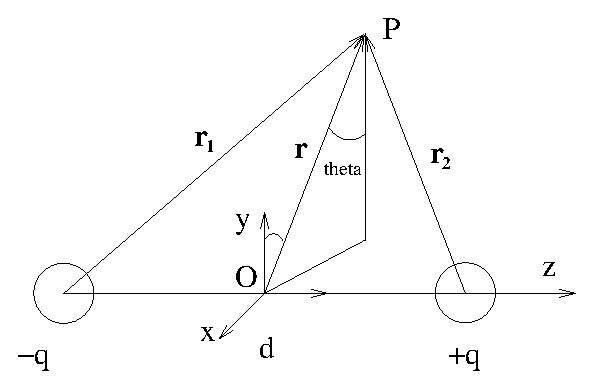
\includegraphics[scale=0.8]{immagini/fisica2/dipolo}
\end{figure}
\subsection{Potenziale}
Consideriamo un dipolo, cioè un sistema di due cariche uguali, con segno opposto, poste ad una distanza $\delta$. Data la simmetria cilindrica usiamo coordinate cilindriche e il potenziale nel punto $P$, individuato dal vettore $\ve r$, non dipende da $\theta$:
\begin{equation}
  \varphi=\varphi(\rho,z)=\frac{1}{4\pi\varepsilon_0}\left\{\frac{-q}{r_1}+\frac{q}{r_2}\right\}
\end{equation}
$r_1$ è la distanza tra il punto $P$ di coordinate $(x,y,z)$ e il punto $A$ di coordinate $(0,0,\delta/2)$, quindi: 
\[
r_2 = \norm{P-A} = \sqrt{x^2+y^2+(z-\delta/2)^2}=\sqrt{\rho^2+(z-\delta/2)^2}
\]
e allora:
\begin{equation}
 \frac{1}{4\pi\varepsilon_0}\left\{\frac{-q}{\sqrt{\left(z+\frac{\delta}{2}\right)^2+\rho^2}}+\frac{q}{\sqrt{\left(z-\frac{\delta}{2}\right)^2+\rho^2}}\right\}
\label{dipolo01}
\end{equation}
I due denominatori della \eqref{dipolo01} li possiamo sviluppare:
\[\left(z^2+\rho^2+\delta z+\frac{\delta^2}{4}\right)^{-\frac{1}{2}}=\left(z^2+\rho^2\right)^{-\frac{1}{2}}\left(1+\frac{\delta z}{\rho^2+z^2}+\frac{\delta^2}{4\left(\rho^2+z^2\right)}\right)^{-\frac{1}{2}}\]
\[\left(z^2+\rho^2-\delta z+\frac{\delta ^2}{4}\right)^{-\frac{1}{2}}=\left(z^2+\rho^2\right)^{-\frac{1}{2}}\left(1-\frac{\delta z}{\rho^2+z^2}+\frac{\delta^2}{4\left(\rho^2+z^2\right)}\right)^{-\frac{1}{2}}\]
se vogliamo considerare $\ve E$ a grande distanza equivale a dire che $\delta$ deve essere molto piccolo, quindi il termine $\delta^2$ non lo consideriamo. Ricordiamo lo sviluppo binomiale:
\[\left(1+x\right)^\alpha=1+\alpha x+\frac{\alpha\left(\alpha-1\right)}{2}x^2+\cdots\]
Allora usando solo il primo ordine:
\[\left(z^2+\rho^2+\delta z+\frac{\delta^2}{4}\right)^{-\frac{1}{2}}\simeq\left(z^2+\rho^2\right)^{-\frac{1}{2}}\left(1-\frac{1}{2}\frac{\delta z}{\rho^2+z^2}\right)\]
\[\left(z^2+\rho^2-\delta z+\frac{\delta^2}{4}\right)^{-\frac{1}{2}}\simeq\left(z^2+\rho^2\right)^{-\frac{1}{2}}\left(1+\frac{1}{2}\frac{\delta z}{\rho^2+z^2}\right)\]
sostituendo nella \eqref{dipolo01}:
\begin{align*}
\varphi&=\varphi(\rho,z)=\frac{1}{4\pi\varepsilon_0}\frac{1}{\sqrt{\rho^2+z^2}}\left\{-q\left(1-\frac{1}{2}\frac{\delta z}{\rho^2+z^2}\right)+q\left(1+\frac{1}{2}\frac{\delta z}{\rho^2+z^2}\right)\right\}\\
&=\frac{q}{4\pi\varepsilon_0}\frac{\delta z}{\left(\rho^2+z^2\right)^\frac{3}{2}}
\end{align*}
che è l'espressione del potenziale del dipolo in coordinate cilindriche. Ma $\sqrt{z^2+\rho^2}=\norm{\ve r}$, definiamo $\ve p=\pm |q|\delta \ver e_z$, con il verso tale che sia diretto dalla carica negativa a quella positiva, momento del dipolo. Essendo $\ve r=\rho\ver e_r+z\ver e_z$ allora $\ve p\cdot\ve r=q\delta z$. In funzione di $\ve r$:
\[\varphi=\varphi(\ve r)=\frac{1}{4\pi\varepsilon_0}\frac{\ve p\cdot\ve r}{{\norm{\ve r}}^3}\]
Dunque il potenziale decresce con $r^2$. Usando $\ve\nabla\left(\frac{1}{r}\right)=-\frac{\ve r}{r^3}$, lo possiamo anche scrivere come:
\begin{equation}
\varphi(\ve r)=-\frac{1}{4\pi\varepsilon_0}\ve p\cdot\ve\nabla\left(\frac{1}{r}\right)
\end{equation}
oppure come:
\begin{equation}
\varphi(\ve r)=-\ve p\cdot\ve\nabla\Phi_0
\end{equation}
con $\Phi_0$ il potenziale sulla carica($\frac{1}{4\pi\varepsilon_0}\frac{1}{r}$). Usando le coordinate cartesiane, $\ve r=x\ver \imath+y\ver \jmath+z\ver k$, $\ve p=p\ver k$:
\begin{equation}
\varphi(x,y,z)=\frac{1}{4\pi\varepsilon_0}\frac{pz}{\left(x^2+y^2+z^2\right)^\frac{3}{2}}
\end{equation}\index{potenziale!elettrostatico!del dipolo}
\subsubsection{Altra dimostrazione}
Immaginiamo una carica $q$ nell'origine, allora il suo potenziale è $\varphi_0\left(\ve r\right)=\frac{1}{4\pi\varepsilon_0}\frac{q}{r}$
spostiamo di $\Delta\ve r=\frac{\ve\delta}{2}$ la carica, allora:
\[\varphi_+\left(\ve r\right)=\varphi_0(\ve r-\Delta \ve r)\simeq\varphi_0-\ve\nabla\varphi_0\cdot\Delta\ve r=\frac{1}{4\pi\varepsilon_0}\frac{q}{r}-\frac{1}{4\pi\varepsilon_0}q\ve\nabla\left(\frac{1}{r}\right)\cdot\frac{\ve\delta}{2}\]
La stessa cosa la possiamo fare con una carica $-q$ e spostarla dall'altra parte $-\Delta\ve r$:
\[\varphi_-\left(\ve r\right)=-\varphi_0(\ve r+\Delta \ve r)\simeq-\varphi_0-\ve\nabla\varphi_0\cdot\Delta\ve r=-\frac{1}{4\pi\varepsilon_0}\frac{q}{r}-\frac{1}{4\pi\varepsilon_0}q\ve\nabla\left(\frac{1}{r}\right)\cdot\frac{\ve\delta}{2}\]
Essendo $\delta\ll r$ allora è una buona approssimazione. Il potenziale totale:
\[\varphi\left(\ve r\right)=\varphi_++\varphi_-=-\frac{1}{4\pi\varepsilon_0}q\ve\nabla\left(\frac{1}{r}\right)\cdot\ve\delta=-\frac{1}{4\pi\varepsilon_0}\ve p\cdot\ve\nabla\left(\frac{1}{r}\right)\]


\subsection{Campo elettrostatico\index{campo!elettrostatico!del dipolo}}
Usando $\ve E=-\grad\varphi$:
\begin{align}
\label{eq:E_dipolo}
E_x&=-\frac{\partial\varphi}{\partial x}=\frac{3pz}{4\pi\varepsilon_0}\frac{x}{\left(x^2+y^2+z^2\right)^\frac{5}{2}}=\frac{3pz}{4\pi\varepsilon_0}\frac{x}{r^5}=\frac{3(\ve p\cdot \ve r)}{\giorgi}\left[\frac{\ve r}{r^5}\right]_x\\
E_y&=-\frac{\partial\varphi}{\partial y}=\frac{3pz}{4\pi\varepsilon_0}\frac{y}{\left(x^2+y^2+z^2\right)^\frac{5}{2}}=\frac{3pz}{4\pi\varepsilon_0}\frac{y}{r^5}=\frac{3(\ve p\cdot \ve r)}{\giorgi}\left[\frac{\ve r}{r^5}\right]_y\\
E_z&=-\frac{\partial\varphi}{\partial z}=\frac{p}{\giorgi}\left(\frac{3z^2}{r^5}-\frac{1}{r^3}\right)=\frac{3(\ve p\cdot \ve r)}{\giorgi}\left[\frac{\ve r}{r^5}\right]_z-\frac{1}{\giorgi}\left[\frac{\ve p}{r^3}\right]_z
\end{align}
definiamo:
\[E_\perp=\sqrt{E_x^2+E_y^2}=\frac{3pz}{4\pi\varepsilon_0}\frac{1}{r^{5}}\sqrt{x^2+y^2}\]
allora:
\[E=\sqrt{E_z^2+E_\perp^2}=\frac{1}{4\pi\varepsilon_0}\frac{p}{r^3}\sqrt{\frac{3z^2}{r^2}+1}=\frac{1}{4\pi\varepsilon_0}\frac{p}{r^3}\sqrt{3\cos^2\theta+1}\]
in forma vettoriale:
\begin{equation}
\label{eq:campo_dipolo}
\ve E(\ve r)=\frac{1}{4\pi\varepsilon_0}\left\{3\left(\ve p\cdot\ve r\right)\frac{\ve r}{r^5}-\frac{\ve p}{r^3}\right\}\end{equation}
Esso decresce con $r^3$ ed è solenoidale, cioè le linee del campo si chiudono. Da questa discende che il flusso su una superficie che racchiude il dipolo è nullo.
\subsection{Energia potenziale\index{energia!potenziale!del dipolo}}
Mettiamo un dipolo in un campo elettrico $\ve E$ esterno. Assumiamo che le due cariche non si muovano. Dove c'è la carica $-q$ ci sia un potenziale esterno $\varphi_A$, nell'altra $\varphi_B$. L'energia potenziale è la somma dell'energia potenziale delle due cariche:
\[W=W_B+W_A=q(\varphi_B-\varphi_A)\]
Calcoliamo il potenziale $\varphi_B$ sviluppando $\varphi_A$ nell'intorno di $\varphi_A$:
\[\varphi_B\simeq\varphi_A+\ve\nabla\varphi\cdot\ve\delta\]
Allora l'energia diventa:
\[W=q\left(\varphi_A+\ve\nabla\varphi\cdot\ve\delta-\varphi_A\right)=q\ve\delta\cdot\ve\nabla\varphi=-\ve p\cdot\ve E\]
Si deduce che la posizione di equilibrio stabile, che corrisponde all'energia minima, si ha quando $\ve p//\ve E$ cioè quando il dipolo è orientato come il campo elettrico esterno. Quando $\ve p$ è antiparallelo al campo elettrico si ha un equilibrio instabile.
\subsection{Forza\index{forza!sul dipolo}}
\label{forza_dipolo100}
\[\ve F=-\ve\nabla W=\ve\nabla\left(\ve p\cdot\ve E\right)=\left(\ve p\cdot\ve\nabla\right)\ve E\]
per esempio:
\[F_x=\left(p_x\frac{\partial E_x}{\partial x}+p_y\frac{\partial E_x}{\partial y}+p_z\frac{\partial E_x}{\partial z}\right)\]
quindi se il campo elettrico esterno è omogeneo allora non c'è forza sul dipolo.
\subsection{Momento\index{momento!sul dipolo}}
\begin{figure}[htbp]
\centering
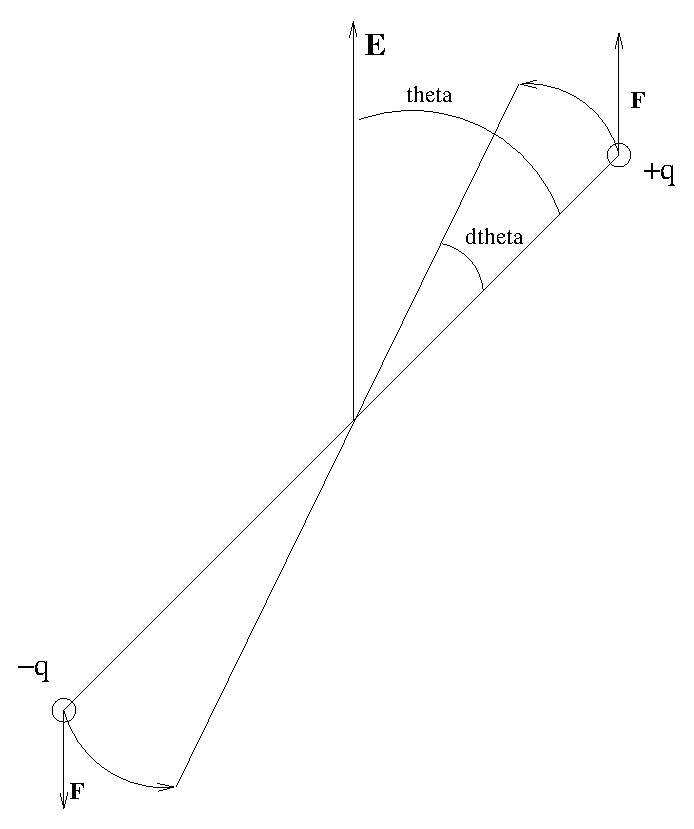
\includegraphics[scale=0.5]{immagini/fisica2/dipolo_mom}
\end{figure}
Il lavoro per far ruotare il sistema di $\ud\theta$ è 
\[\delta L=-M\ud\theta\]
notare che $\theta$ diminuisce, quindi la sua variazione è negativa. Essendo il sistema isolato il lavoro compiuto deve tramutarsi in variazione di energia potenziale:
\[\ud W=\delta L=M\ud\theta\]
Allora:
\[M=\frac{\ud W}{\ud\theta}=\frac{-pE\cos\theta}{\ud\theta}=pE\sin\theta\]
\[\ve M=\ve p\times\ve E\]
che fa ruotare il dipolo fino alla posizione di equilibrio. Questa relazione può essere calcolata semplicemente dalla definizione di momento torcente:
\[
 \ve M = \ve r_+\times \ve F_+ + \ve r_-\times\ve F_- = q(\ve r_+-\ve r_-)\times \ve E=\ve p\times\ve E
\]

\subsection{Interazione dipolo-dipolo}
Consideriamo due dipoli $\ve p_1$ e $\ve p_2$. Vogliamo sapere come interagiscono. Calcoliamo prima l'energia potenziale del sistema. Il campo generato del primo dipolo è:
\[
 \ve E_1 = \frac{1}{\giorgi}\left(3(\ve p_1\cdot \ve r)\frac{\ve r}{r^5}-\frac{\ve p_1}{r^3}\right)
\]
quindi l'energia di interazione è:
\[
 U = -\ve E_1\cdot \ve p_2 = \frac{1}{\giorgi}\left(3\frac{(\ve p_1\cdot \ve r)(\ve p_2\cdot \ve r)}{r^5}-\frac{\ve p_1\cdot\ve p_2}{r^3}\right)
\]
che varia come $\frac{1}{r^3}$. Quest'interazione è quella che si verifica tra molecole neutre ma polari, che presentano un momendo di dipolo, come l'acqua.
\index{dipolo|)}
\section{Sviluppo in multipoli\index{multipoli|(}\index{sviluppo!in multipoli|(}}
Il multipolo è un sistema formato da diverse cariche. Ci interessa sapere come si comporta $\varphi$ a grande distanza. Una distribuzione di cariche può essere approssimata a grande distanza da sovrapposizione di multipoli.
\subsection{Distribuzione di carica}
Immaginiamo una distribuzione di carica nello spazio con densità $\rho(x,y,z)$. Sia l'origine all'interno della distribuzione. Il potenziale totale è 
\begin{equation}
\varphi(\ve r)=\frac{1}{4\pi\varepsilon_0}\int_V\frac{\rho(\ve r\,')\ud v}{\norm{\ve r-\ve r\,'}}
\label{multipolo_01}
\end{equation}
\begin{center}
$
\xymatrix{
&&C&&&\\
\\
\\
A\ar[rruuu]^{\ve r}\ar[rrrrr]^{\ve r\,'}&&&&&B\ar[llluuu]_{\ve r-\ve r\,'}
}$\end{center}
Usando il teorema dei coseni possiamo scrivere:
\[\norm{\ve r-\ve r\,'}=\sqrt{r^2+r'^2-2\ve r\cdot \ve r\,'}=r\sqrt{1+\frac{r'^2}{r^2}-\frac{2\ve r\cdot \ve r\,'}{r^2}}\]
Ricordando che:
\[(1+\varepsilon)^{-\frac{1}{2}}=1-\frac{1}{2}\varepsilon+\frac{3}{8}\varepsilon^2+\cdots\]
si ha:
\begin{align*}
{\norm{\ve r-\ve r\,'}}^{-1}=&\frac{1}{r}\left(1+\frac{r'^2}{r^2}-\frac{2\ve r\cdot \ve r\,'}{r^2}\right)^{-\frac{1}{2}}\\
=&\frac{1}{r}\left\{1+\frac{\ve r\cdot\ve r\,'}{r^2}-\frac{1}{2}\frac{r'^2}{r^2}+\frac{3}{8}\left[\frac{2\ve r\cdot\ve r\,'}{r^2}-\frac{r'^2}{r^2}\right]^2+o\left(\frac{r'}{r}\right)^2\right\}\\
=&\frac{1}{r}\left\{\underbrace{1}_{\sim 1}+\underbrace{\frac{\ve r\cdot\ve r\,'}{r^2}}_{\sim x}-\underbrace{\frac{1}{2}\frac{r'^2}{r^2}}_{\sim x^2}+\underbrace{\frac{3}{8}\left(\frac{r'}{r}\right)^4}_{\sim x^4}-\underbrace{\frac{3}{8}\left(\frac{r'}{r}\right)^2\frac{\ve r\cdot \ve r'}{r^3}}_{\sim x^3}+\underbrace{\frac{3}{2}\frac{(\ve r\cdot \ve r')}{r^4}}_{x^2}+\underbrace{o\left(\frac{r'}{r}\right)^2}_{o(x^2)}\right\}\\
\simeq&\frac{1}{r}+\frac{\ve r\cdot\ve r\,'}{r^3}+\frac{1}{2}\left[-\frac{r'^2}{r^3}+\frac{3\left(\ve r\cdot\ve r\,'\right)^2}{r^5}\right]\\
\end{align*}
Nell'ultimo passaggio abbiamo considerato che $r\gg r'$. Sostituendo l'ultimo risultato nella \eqref{multipolo_01} si ottiene:
\begin{multline}
\label{multipolo02}
\varphi(\ve r)\simeq\frac{1}{4\pi\varepsilon_0}\left\{\frac{1}{r}\int_V\rho(\ve r\,')\,\ud v+\frac{\ve r}{r^3}\cdot\int_V\rho(\ve r\,')\ve r\,'\,\ud v+\right.\\
\left.+\frac{1}{2}\int_V\rho(\ve r\,')\left[\frac{3\left(\ve r\cdot\ve r\,'\right)^2}{r^5}-\frac{r'^2}{r^3}\right]\,\ud v\right\}
\end{multline}
Analizziamo i termini della \eqref{multipolo02}. Il primo:
\[\frac{1}{4\pi\varepsilon_0}\frac{1}{r}\int_V\rho(\ve r\,')\,\ud v=\frac{1}{4\pi\varepsilon_0}\frac{Q}{r}\]
è il potenziale di un monopolo, cioè il potenziale di un punto in cui è accumulata tutta la carica della distribuzione. A grande distanza è un'approssimazione accettabile. Il secondo termine corregge il precedente:
\[\frac{1}{4\pi\varepsilon_0}\frac{\ve r}{r^3}\cdot\int_V\rho(\ve r\,')\ve r\,'\,\ud v\]
è il potenziale di un dipolo, infatti possiamo definire:
\[\ve p=\int_V\rho(\ve r\,')\ve r\,'\ud v\]
momento di dipolo della distribuzione di carica. Gli altri termini sono i potenziali di quadripolo, ottupolo, \ldots Notare che:
\begin{equation}
\ve\delta=\frac{\ve p}{|q|}=\frac{\int_V\rho(\ve r\,')\ve r\,'\ud v}{|q|}
\end{equation}
individua il centro di \index{centro!di carica}carica.\index{sviluppo!in multipoli|)}\index{multipoli|)}
\begin{Es}[Doppio anello]
 Siano due anelli sottili di raggio $R$ nel piano $x$--$y$ ad altezza $z=\pm\frac{d}{2}$ e con il centro sull'asse $z$. Gli anelli sono uniformemente carichi con densità lineare $\pm\lambda$. Calcolare il campo elettrico totale lungo l'asse $z$, fare un'approssimazione per $|z|\gg d,R$.
\begin{figure}[htbp]
 \centering
 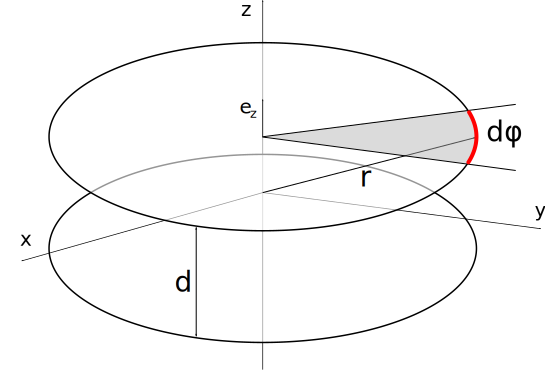
\includegraphics[scale=0.5]{immagini/fisica2/due_anelli_schema}
 % due_anelli_schema.pdf: 436x297 pixel, 72dpi, 15.38x10.48 cm, bb=0 0 436 297
\end{figure}

Il campo elettrico può essere trovato con il principio di sovrappossizione, calcolando separatamente i campi generati da ciascun anello. Come calcolato nell'esempio \ref{es:anello} il campo elettrico generato da un anello nell'origine lungo il suo asse è:
\begin{align*}
 \ve E_0(0,0,z)&=\frac{q}{4\pi\varepsilon_0}\frac{z}{(R^2+z^2)^{\frac{3}{2}}}\ver e_z\\
             &=\frac{\lambda R}{2\varepsilon_0}\frac{z}{(R^2+z^2)^{\frac{3}{2}}}\ver e_z
\end{align*}
quindi il campo elettrico generato dai due anelli è:
\begin{align*}
 \ve E(0,0,z)&=\ve E_{+\frac{d}{2}}+\ve E_{-\frac{d}{2}}\\
               &=\frac{\lambda R}{2\varepsilon_0}\left\{
                  \frac{z-\frac{d}{2}}{\left[R^2+(z-\frac{d}{2})^2\right]^{\frac{3}{2}}}
                 -\frac{z+\frac{d}{2}}{\left[R^2+(z+\frac{d}{2})^2\right]^{\frac{3}{2}}}\right\}\ver e_z
\end{align*}
Per ottenere un'appossimazione per $|z|\gg d,R$ possiamo fare uno sviluppo di Taylor:
\begin{multline*}
 \frac{z-\frac{d}{2}}{\left[R^2+(z-\frac{d}{2})^2\right]^{\frac{3}{2}}}
=\frac{z}{|z|^3}\frac{(1-\frac{d}{2z})}{\left[\underbrace{\left(\frac{R}{z}\right)^2}_{\simeq 0}+\left(1-\frac{d}{2z}\right)^2\right]^{3/2}}\\
\simeq\frac{\sgn{z}}{z^2}\left(1-\frac{d}{2z}\right)\left(1+\frac{3d}{2z}\right)
\simeq\frac{\sgn{z}}{z^2}\left(1+\frac{d}{z}\right)
\end{multline*}
La semplificazione $\left(\frac{R}{z}\right)^2\simeq 0$ e anche quella nell'ultimo passaggio sono giustificate dal fatto che la nostra espanzione è al primo grado. Quindi la nostra approssimazione per il campo elettrostatico:
\[
 \ve E(0,0,z) \simeq \frac{\lambda R}{2\varepsilon_0}\frac{\sgn{z}}{z^2}\left\{\left(1+\frac{d}{z}\right)-\left(1-\frac{d}{z}\right)\right\}\ver e_z
 = \frac{\lambda R}{\varepsilon_0}\frac{d}{|z|^3}\ver e_z
\]
Notiamo che la dipendenza da $\frac{1}{r^3}$ è tipica dei dipoli \eqref{eq:campo_dipolo}, infatti il sistema è approssimabile con un dipolo che punta dall'anello negativo a quello positivo:
\[
 \ve p = \int_\Gamma \ve r\,\ud q = \int_{\Gamma_+} \left\{\frac{d}{2}\ver e_z+R\ver u_r\right\}\left(\lambda R\ud\phi\right) + \int_{\Gamma_-} \left\{-\frac{d}{2}\ver e_z+R\ver u_r\right\}\left(-\lambda R\ud\phi\right)
\]
spezzando gli integrali le parti che contengono $\ver u_r$ si annullano, in quando la somma di tutti i versori radiali, al variare dell'angolo $\phi$ fa il vettore nullo.
\[
 \ve p = 2\pi\lambda R d\ver e_z
\]
questo vuol dire che il nostro sistema è assimilabile a un sistema di due cariche di carica $\pm 2\pi\lambda R $ e distanti $d$, quindi come se fossero messe nel centro degli anelli. Usando l'espressione del campo elettrico generato da un dipolo \eqref{eq:campo_dipolo}:
\begin{align*}
 \ve E(0,0,z) &= \frac{1}{\giorgi}\left\{3(\ve p\cdot\ve r)\frac{\ve r}{r^5}-\frac{\ve p}{r^3}\right\}\\
              &= \frac{1}{\giorgi}\left\{3(2\pi\lambda R d\ver e_z\cdot z\ver e_z)\frac{z\ver e_z}{|z|^5}-\frac{2\pi\lambda R d\ver e_z}{|z|^3}\right\}\\
              &= \frac{\lambda R}{\varepsilon_0}\frac{d}{|z|^3}\ver e_z
\end{align*}
avendo usato $\ve r=z\ver e_z$ e quindi $r = |z|$.
\begin{figure}[htbp]
 \centering
 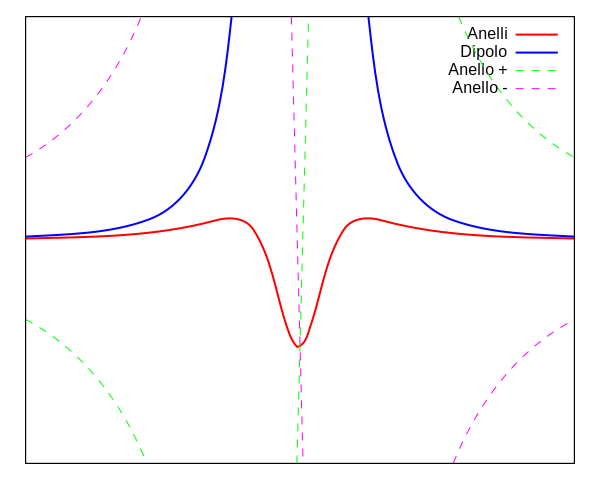
\includegraphics[scale=0.5]{immagini/fisica2/due_anelli}
 % due_anelli.pdf: 480x384 pixel, 72dpi, 16.93x13.55 cm, bb=0 0 480 384
 \caption{campo elettrostatico di due anelli lungo l'asse $z$ (esatto, approssimazione di dipolo e anelli singoli).}
\end{figure}
\end{Es}
\begin{Es}[Doppio anello 2]
  Calcolare il lavoro che deve essere fatto dall'esterno per portare una carica $e$ da un punto infinitamente lontano all'origine. Calcolare il lavoro che dev'essere fatto per portare un dipolo $\ve p$ con il verso lungo l'asse $z$ da un punto infinitamente lontano all'origine.

  Il lavoro fatto dall'esterno può calcolare come variazione dell'energia potenziale:
  \[
   L_\text{ext} = e(\varphi(0)-\varphi(\infty))
  \]
   Per valutare il potenziale al posto di fare la derivata del campo lo si può calcolare dalla definizione. Il potenziale generato da una spira sull'asse è:
  \[
   \varphi_0 = \frac{1}{\giorgi}\int\frac{\ud q}{\norm{\ve r - \ve r'}} = \frac{1}{\giorgi}\int_0^{2\pi}\frac{\lambda R\ud\phi}{\left[R^2+\left(z-\frac{d}{2}\right)^2\right]^{1/2}}=\frac{\lambda R}{2\varepsilon_0}\frac{1}{\sqrt{z^2+R^2}}
  \]
   quindi il potenziale dei due anelli:
  \[
   \varphi = \varphi_{+\frac{d}{2}} - \varphi_{-\frac{d}{2}} = \frac{\lambda R}{2\varepsilon_0}\left\{\frac{1}{\sqrt{\left(z-\frac{d}{2}\right)^2+R^2}}-\frac{1}{\sqrt{\left(z+\frac{d}{2}\right)^2+R^2}}\right\}
  \]
  poiché $\varphi(0)=0$ e $\varphi(\infty)=0$ il lavoro è nullo. Alla conclusione che $\varphi(0)=0$ ci si poteva arrivare anche con ragionamenti sulla simmetria del sistema. Infatti sicuramente $\varphi_0(z) = \varphi(-z)$ quindi
  \[
  \begin{aligned}
   \varphi(z=0) &= \left[\varphi_0(z+d/2)-\varphi_0(z-d/2)\right]_{z=0} \\
		&= \varphi_0(d/2)-\varphi_0(-d/2) = \varphi_0(d/2)-\varphi_0(d/2) = 0
  \end{aligned}
  \]


  Il lavoro fatto per spostare il dipolo si può fare in maniera analoga, ricordando che l'energia potenziale di un dipolo che interagisce con un campo elettromagnetico è $-\ve p\cdot \ve E$.
  \begin{align*}
   W(0) &= -\ve p\cdot \frac{\lambda R}{2\varepsilon_0}\left\{
                  \frac{z-\frac{d}{2}}{\left[R^2+\left(z-\frac{d}{2}\right)^2\right]^{\frac{3}{2}}}
                 -\frac{z+\frac{d}{2}}{\left[R^2+\left(z+\frac{d}{2}\right)^2\right]^{\frac{3}{2}}}\right\}_{z=0}\ver e_z\\
        &= p\frac{\lambda R}{2\varepsilon_0}
                  \frac{d}{\left[R^2+\left(\frac{d}{2}\right)^2\right]^{\frac{3}{2}}}
  \end{align*}
essendo $W(\infty)=0$ questo è già il lavoro.
\end{Es}



\chapter{Elettrostatica nei conduttori\index{elettrostatica!nei conduttori}}
\minitoc
\section{Conduttori ed isolanti\index{conduttori}\index{isolanti}}
Dal punto di vista elettrico i materiali possono essere divisi in due categorie:
\begin{description}
\item[conduttori] hanno molte cariche elettriche libere, una nuvola elettronica con densità constante in condizioni standard;
\item[isolanti] hanno atomi e molecole molto legati tra di loro che atomi tendono a deformarsi sotto l'effetto di un campo elettrico;
\end{description}
I materiali si caratterizzano per tre costanti:
\begin{itemize}
\item conducibilità elettrica $\sigma$, descrive la risposta dei suoi elettroni soggetti a un campo elettrico esterno;
\item costante dielettrica $\varepsilon$;
\item permeabilità magnetica $\mu$;
\end{itemize}

\section{Carica nei conduttori}
Se carichiamo un conduttore gli elettroni dopo una frazione di tempo trovano una condizione di equilibrio e quindi il campo elettrostatico all'interno del conduttore deve essere nullo. Essendo il campo il gradiente del potenziale allora se il campo è nullo il potenziale è costante e quindi il conduttore è un corpo equipotenziale e in particolare la sua superficie è equipotenziale. Usando il teorema di Gauss, con superfici gaussiane che tendono al bordo scopriamo che all'interno non ci possono essere cariche, allora per la conservazione della carica esse sono sul bordo. Il campo elettrostatico all'esterno è ortogonale alla superficie essendo essa una superficie equipotenziale, inoltre se esso avesse una componente tangenziale le cariche al suo interno si muoverebbero.
\section{Induzione elettrostatica}
\begin{Def}[Induzione elettrostatica\index{induzione elettrostatica}]
L'induzione elettrostatica è quel fenomeno per cui in presenza di un campo elettrico esterno le cariche libere in un conduttore si ridistribuiscono.
\end{Def}
Se mettiamo un conduttore in uno spazio in cui è presente un campo elettrico $\ve E_\text{ext}$ gli elettroni al suo interno si muovono in senso opposto ad $\ve E_\text{ext}$. In questo modo creano un accumulo di cariche che a sua volta crea un campo elettrico indotto dalla carica migrata $\ve E_i$. In pochissimo tempo gli elettroni arrivano ad un a posizione di equilibrio in cui:
\[\ve E=\ve E_i+\ve E_\text{ext}=0\]
Possiamo allora affermare che (a parte il brevissimo istante in cui le cariche creano raggiungono l'equilibrio) il campo elettrico totale all'interno di un conduttore ideale è nullo. Anche il campo esterno risulta deformato dalla nuova distribuzione di cariche e a grande distanza torna ad essere quello in assenza di distribuzione di cariche. Se il campo elettrico all'interno è nullo le cariche devono essersi accumulate sul bordo del conduttore, infatti:
consideriamo una superficie chiusa completamente compresa nel conduttore; essendo il campo interno nullo, per il teorema di Gauss, anche la carica deve essere nulla. Facciamo tendere questa superficie alla superficie del conduttore, la carica è sempre nulla. Per la conservazione della carica questa può essere solo sul bordo del conduttore.

\section{Teorema di Coulomb\index{Coulomb}\index{teorema!di Coulomb}}
Vogliamo calcolare il campo elettrico in prossimità della superficie del conduttore. Sappiamo già che questo è perpendicolare alla superficie. Sulla superficie si è distribuita una densità superficiale di carica $\sigma$ a causa del campo elettrico esterno, tale che $\int_S \sigma\ud a=Q$. Ipotizziamo che $Q=0$, cioè il conduttore sia inizialmente scarico.

Consideriamo un cilindretto di basi infinitesime $\ud A$, una interna e l'altra esterna al conduttore, perpendicolare alla superficie del conduttore. Il flusso attraverso la superficie laterale è nullo in quanto $\ve E\perp\ve n$, e anche il flusso attraverso la superficie interna al conduttore è nullo perché qui il campo è nullo. Rimane solo la superficie all'esterno del conduttore, per Gauss:
\[\int_{S_1}\ve E\cdot\ve n\,\ud a=\frac{q}{\varepsilon_0}=\frac{\sigma\Delta a}{\varepsilon_0}\]
ma $\ve E//\ve n$ ed è costante: $\int_{S_1}\ve E\cdot\ve n=E\Delta S_1$ e $\Delta a = \Delta S_1$:
\begin{Teo}[Coulomb]
In prossimità di un conduttore il campo elettrico totale è 
\begin{equation}
 \label{eq:teo_coulomb}
 E=\frac{\sigma}{\varepsilon_0}
\end{equation}
\end{Teo}

Potrebbe sorgere un dubbio. Se usiamo il teorema di Coulomb su un piano infinito troveremmo una contraddizione. Infatti sappiamo che il campo di un piano infinito è $E=\frac{\sigma}{2\varepsilon_0}$ esattamente la metà di quanto direbbe il teorema di Coulomb. Torniamo al teorema di Coulomb: consideriamo un elementino $\Delta S$ di area $\Delta A$, vogliamo sapere il campo generato da questo elementino in prossimità del conduttore. Questo significa fare il limite del campo per la distanza che tende a zero. Se prendiamo un punto e andiamo infinitamente vicino a $\Delta S$ allora $\Delta A$ sarà vista dal punto come infinita e allora il campo varrà in prossimità $E=\frac{\sigma}{2\varepsilon_0}$ sia all'esterno che all'interno. Ma sappiamo che all'interno il campo deve essere nullo, allora tutti gli altri elementini $S-\Delta S$ devono generare un campo che annulli il campo interno e raddoppino quello esterno in modo tale che $E=\frac{\sigma}{\varepsilon_0}$.

\subsection{Pressione elettrostatica\index{pressione!elettrostatica}}
Consideriamo un conduttore carico. Le cariche si distribuiranno sulla superficie. Consideriamo due punti $A$ e $B$ in prossimità di un elementino $\ud a$ della superficie del conduttore. $A$ sia esterno, $B$ interno. Il campo su $A$ è la somma del campo $\ve E_1$ generato dalle cariche appartenenti all'area $\ud a$ e $\ve E_2$ generato dalle cariche distribuite sul resto della superficie. Lo stesso per un punto $B$ interno al conduttore. Mentre però passando da $A$ a $B$ il campo $\ve E_2$ rimane pressoché costante, $\ve E_1$ cambia di verso. Dunque:
\[\ve E_A=\ve E_1+\ve E_2=\frac{\sigma}{\varepsilon_0}\ve n\]
\[\ve E_B=-\ve E_1+\ve E_2=0\]
Infatti $B$ è all'interno del conduttore. Dalle precedenti ricaviamo:
\[\ve E_2=\ve E_1=\frac{\sigma}{2\varepsilon_0}\ve n\]
Sulle cariche su $\ud a$ la forza è 
\[\ud \ve F=\left(\frac{1}{2}\frac{\sigma}{\varepsilon_0}\ve n\right)\sigma\ud a\]
La forza sull'unità di area è detta pressione elettrostatica:
\begin{equation}
P=\frac{\ud(\ve F\cdot \ve n)}{\ud a}=\frac{1}{2}\frac{\sigma^2}{\varepsilon_0}
\end{equation}
naturalmente con verso verso l'esterno. Le forze tendono quindi a strappare le cariche verso l'esterno. Servono campi molto intensi per far uscire le cariche dal conduttore.
\subsubsection{Terra\index{terra}}
\label{potenziale_terra}
La terra è considerato come un enorme conduttore, così grande che non riusciamo a modificarne le caratteristiche elettrostatiche. \`E l'analogo termodinamico del bagno termico. Ad essa si attribuisce il valore di potenziale zero. Allora il potenziale possiamo definirlo come il lavoro necessario per portare una carica unitaria dalla terra al punto.
\subsection{Induzione tra conduttori}
Se avvicino un corpo $A$ carico a un $B$ scarico, le cariche su $B$ si ridistribuiscono in modo tale che il campo totale all'interno di $B$ sia nullo. Le cariche su $B$ si dicono indotte. Ora anche $B$ produce un campo elettrico all'esterno che induce una distribuzione di carica su $A$. Il tutto fino al raggiungimento di un equilibrio. Se ora colleghiamo $B$ con la terra, il conduttore $B$ e la terra diventano un unico conduttore; allora le cariche si distribuiranno sulla superficie di questo unico conduttore. Se stacchiamo la terra, $B$ risulta carico.
\begin{figure}[htbp]
\centering
\subfigure[$B$ scarico]{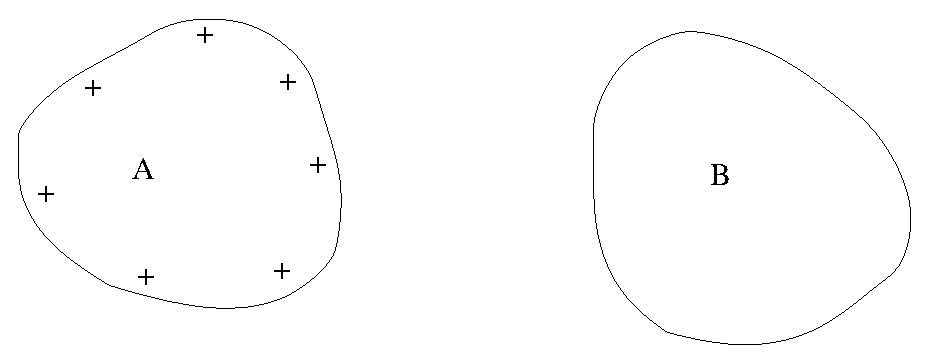
\includegraphics[scale=0.42]{immagini/fisica2/induz1}}
\qquad
\subfigure[$A$ induce delle cariche su $B$]{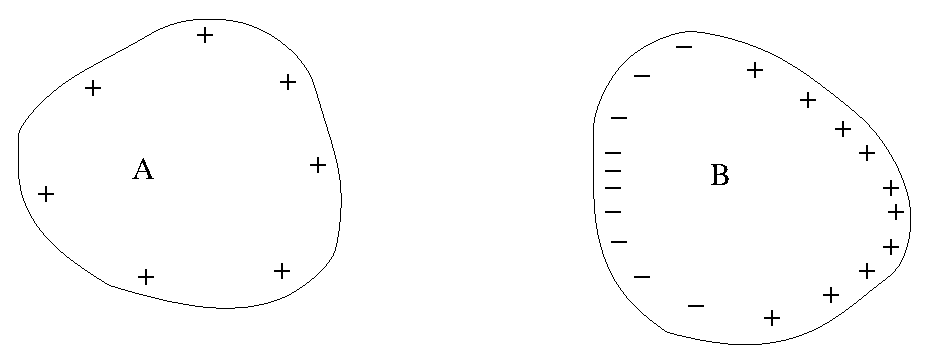
\includegraphics[scale=0.42]{immagini/fisica2/induz2}}
\subfigure[$B$ modifica la distribuzione delle cariche su $A$]{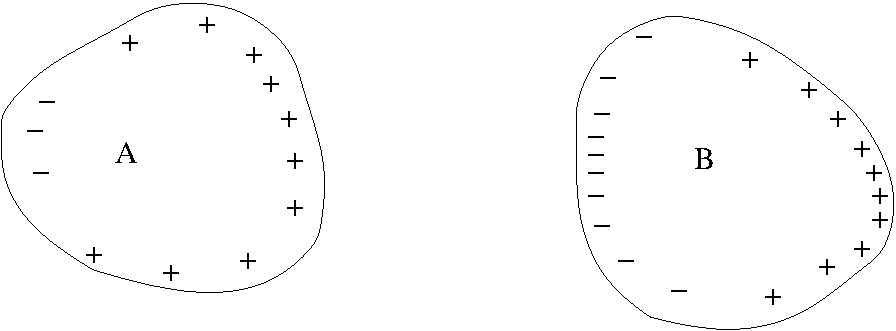
\includegraphics[scale=0.4]{immagini/fisica2/induz3}}
\qquad
\subfigure[$B$ è collegato a terra, formano un unico conduttore]{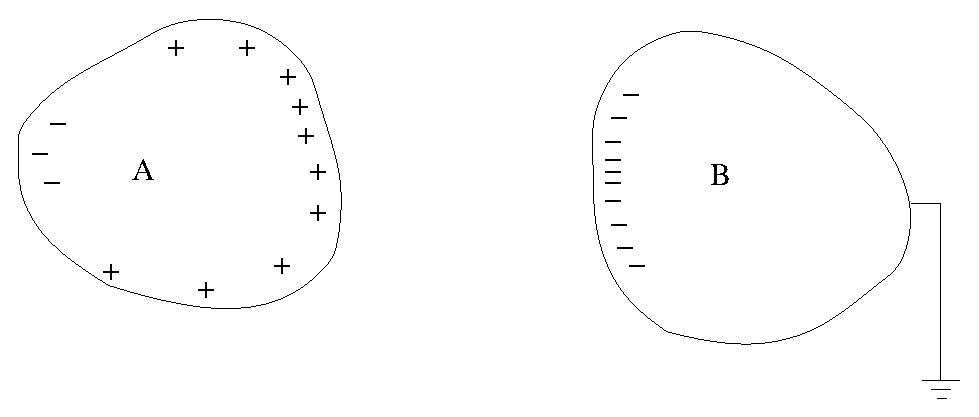
\includegraphics[scale=0.40]{immagini/fisica2/induz4}}\\
\subfigure[$B$ da solo è carico]{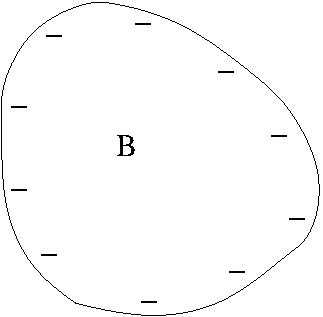
\includegraphics[scale=0.43]{immagini/fisica2/induz5}}
\caption{Induzione elettrostatica.}
\end{figure}
\subsection{Induzione completa\index{induzione elettrostatica!completa}}
Consideriamo un conduttore cavo scarico. Poniamo all'interno del conduttore una carica $q$. Applichiamo il teorema di Gauss all'interno del conduttore. Il campo è zero, allora la carica totale interna al condensatore è nulla. Facendo tendere la superficie gaussiana alla superficie interna si scopre che ci deve essere una carica $-q$ sulla parete interna del conduttore che bilancia la carica $q$ interna, in modo che la carica totale interna alla superficie gaussiana sia nulla. Sulla superficie esterna invece ci deve essere una carica $q$ in modo che il corpo sia ancora complessivamente scarico. La carica indotta è uguale alla carica inducente. Questo fenomeno avviene solo quando il corpo inducente è totalmente racchiuso dal corpo indotto.
\begin{Es}[schermo elettrostatico\index{schermo elettrostatico} -- lo smerdatore]
Im\-ma\-gi\-nia\-mo una fanciulla rinchiusa dentro un conduttore cavo. Adamo, all'esterno, ha molta voglia di sperimentare. Prova a farsi notare avvicinando una carica positiva al conduttore. Sull'esterno si accumula una carica negativa, all'interno positiva. La fanciulla non si accorge di niente essendo il campo elettrico interno invariato. La fanciulla, tutta sola, prova a farsi notare, agitando una carica positiva. Sulla parete interna si crea un accumulo di cariche positive, all'esterno negative, ma Adamo non percepisce nessuna variazione del campo elettrostatico. Il conduttore cavo funziona da schermo elettrostatico.
\end{Es}
\section{Potere dispersivo delle punte\index{potere dissipativo delle punte}}
In un conduttore carico la densità di carica sugli spigoli è maggiore che altrove. Consideriamo una punta carica nell'atmosfera vicino ad una candela. Si osserva che la fiamma oscilla a causa di un vento ionico. Infatti la carica sul conduttore attira ioni dell'atmosfera di segno opposto che lentamente neutralizzano la carica sul conduttore e contemporaneamente respinge gli ioni con lo stesso segno.. Si crea così un movimento di cariche, in questo caso particelle cariche dell'aria che muovono la fiamma. Per spiegare il fenomeno interpretiamo gli spigoli come zone dove il raggio di curvatura è più piccolo. Consideriamo allora due sfere cariche con raggi diversi $R>r$ collegate a grande distanza (niente induzione) da un filo. Sulla prima sfera:
\[V_1=\frac{1}{4\pi\varepsilon_0}\oint_{S_1}\frac{\sigma_R\ud a}{\norm{\ve r-\ve r\,'}}=\frac{1}{4\pi\varepsilon_0}\oint_{S_1}\frac{\sigma_R\ud a}{R}=\frac{1}{4\pi\varepsilon_0}\frac{\sigma_R}{R}4\pi R^2=\frac{\sigma_R R}{\varepsilon_0}=\frac{Q}{4\varepsilon_0\pi R}\]
Sulla seconda:
\[V_2=\frac{1}{4\pi\varepsilon_0}\oint_{S_2}\frac{\sigma_r\ud a}{\norm{\ve r-\ve r\,'}}=\frac{1}{4\pi\varepsilon_0}\oint_{S_2}\frac{\sigma_r\ud a}{r}=\frac{1}{4\pi\varepsilon_0}\frac{\sigma_r}{r}4\pi r^2=\frac{\sigma_r r}{\varepsilon_0}=\frac{q}{4\varepsilon_0\pi r}\]
ma $V_1=V_2$ perché un unico conduttore, allora:
\begin{equation}
\frac{Q}{R}=\frac{q}{r}
\label{candela01}
\end{equation}
La carica è proporzionale al raggio, la densità superficiale di carica:
\[\sigma_R=\frac{Q}{4\pi R^2}\qquad \sigma_r=\frac{q}{4\pi r^2}\]
Allora il rapporto tra le densità di carica (usando la precedente e la \eqref{candela01}):
\[\frac{\sigma_R}{\sigma_r}=\frac{Qr^2}{qR^2}=\frac{r}{R}<1\]
Dunque $\sigma_R<\sigma_r$ e, per il teorema di Coulomb, in prossimità dei conduttori:
\[E_r>E_R\]
\section{Capacità elettrica\index{capacità elettrica}}
Consideriamo un conduttore isolato. Carichiamolo con una carica $q$; il conduttore raggiungerà un certo pontenziale:
\[\varphi(\ve r)=\frac{1}{4\pi\varepsilon_0}\int_S\frac{\sigma(\ve r\,')\,\ud a'}{\norm{\ve r-\ve r\,'}}\]
Se aggiungiamo ancora $q$ arrivando a $2q$ anche il potenziale raddoppia. Si definisce:
\begin{Def}[capacità di un conduttore]
\begin{equation}
C=\frac{q}{V}
\end{equation}
\end{Def}
Esso è costante, dipende solo dalla geometria del conduttore. Si misura in $\text{farad}=\farad=\frac{\text{coulomb}}{\text{volt}}$.
\begin{Es}[sfera]
Calcoliamo la capacità di una sfera conduttrice di raggio $R$. Sapendo che la carica si distribuisce uniformemente per simmetria:
\[\sigma(\ve r)=\frac{Q}{4\pi R^2}=\sigma\]
\[\varphi(\ve r)=\frac{1}{4\pi\varepsilon_0}\oint_S\frac{\sigma(\ve r\,')\,\ud a'}{R}=\frac{1}{4\pi\varepsilon_0}\frac{Q}{4\pi R^2 R}4\pi R^2=\frac{1}{4\pi\varepsilon_0}\frac{Q}{R}\]
\[C=\frac{Q}{\varphi}=4\pi\varepsilon_0R\]
Se $R=\si{1}{\metre}$ allora $C=\si{1E-10}{\farad}$. Il farad è un'unità generalmente grande.
\end{Es}
\subsection{Condensatore}
Mettere troppa carica su un conduttore è difficile perché questa tende a dissiparsi nell'aria. \`E invece più pratico aumentare la capacità 

Usiamo due conduttori, sia $A$ carico e quindi con un certo potenziale $V_0$ e $B$ scarico. $A$ induce delle cariche su $B$ e $B$ modifica la distribuzione delle cariche di $A$. Ora il potenziale di $A$ $V_A$ è minore del potenziale iniziale, a causa delle cariche di segno opposto sul lato di $B$ rivolto verso $A$. Quindi $V_A<V_0$ e allora se all'inizio $C=\frac{Q}{V_0}$ e ora $C'=\frac{Q}{V_A}$ e la carica $Q$ è costante si ha che $C'>C$. Abbiamo aumentato la capacità del condensatore.
\begin{Def}[condensatore]
Il condensatore è un sistema formato da due conduttori adiacenti, isolati, carichi, con cariche di uguale valore, ma di segno opposto e tali da subire la stessa influenza elettrostatica da parte di altri conduttori.
\end{Def}
\begin{figure}[htbp]
\centering
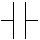
\includegraphics[scale=1.5]{immagini/fisica2/cond1}
\caption{simbolo del condensatore.}
\end{figure}
Se colleghiamo il corpo $B$ a terra otteniamo un condensatore. I due conduttori sono chiamati piatti o armature del condensatore.
\begin{Def}[carica del condensatore]
La carica del condensatore è il valore assoluto della carica immagazzinata da uno dei due conduttori di un condensatore.
\end{Def}
\begin{Def}[capacità del condensatore]
\[C=\frac{Q}{\Delta V}\]
con $Q$ la carica del condensatore e $\Delta V$ la differenza di potenziale tra le due armature.
\end{Def}
Essa dipende solo dalla geometria del condensatore.
\subsubsection{Esempi di geometrie}
\begin{Es}[piano]
Consideriamo due lastre infinite $A$ e $B$ parallele, a distanza $d$. La carica si distribuisce uniformemente:
\[\sigma=\frac{Q}{S}\]
Il campo del condensatore è 
\[\ve E=\frac{\sigma}{\varepsilon_0}\ver \imath\]
\[\Delta V=V_B-V_A=-\int_A^B\ve E\cdot\ud l=-\ve E\int_A^B\ud l=-\frac{\sigma}{\varepsilon_0}d\]
\[C=\frac{Q}{\Delta V}=\frac{\sigma S}{\sigma d}\varepsilon_0=\frac{S}{d}\varepsilon_0\]
Da questo esempio si deduce che $\varepsilon_0$ si può esprimere in $\farad\per\meter$.
\end{Es}
\begin{Es}[sferico]
Consideriamo due sfere con raggi $a<b$ concentriche. Sia $q$ la carica del condensatore. Il campo all'interno può essere calcolato con Gauss. Pensiamo una superficie gaussiana sferica con raggio $r:a<r<b$ concentrica al condensatore. Allora:
\[\Phi_S(\ve E)=E 4\pi r^2=\frac{Q}{\varepsilon_0}=\frac{q}{\varepsilon_0}\qquad \ve E=\frac{1}{4\pi\varepsilon_0}\frac{q}{r^2}\ver e_r\]
diretto radialmente, il verso è dato dal segno di $q$. Calcoliamo la differenza di potenziale tra le due sfere scegliendo un percorso $\Gamma$ radiale:
\[\Delta V=\int_\Gamma\ve E\cdot\ud\ve s=\int_\Gamma E\ud r=\frac{q}{4\pi\varepsilon_0}\int_a^b\frac{1}{r^2}\ud r=\frac{q}{4\pi\varepsilon_0}\left(\frac{1}{a}-\frac{1}{b}\right)\]
\[C=\frac{q}{\Delta V}=\frac{q4\pi\varepsilon_0}{q}\left(\frac{ab}{b-a}\right)=4\pi\varepsilon_0\frac{ab}{b-a}\]
\end{Es}
\begin{Es}[cilindrico]
Consideriamo un condensatore formato da due cilindri coassiali con raggi $a<b$ e altezza $h$. Sia $q$ la carica del condensatore. Per calcolare il campo serviamoci di una superficie gaussiana cilindrica coassiale di altezza $h$ con raggio $r:a<r<b$, consideriamo il condensatore infinito:
\[\Phi_S(\ve E)=E2\pi rh=\frac{Q}{\varepsilon_0}=\frac{q}{\varepsilon_0}\qquad \ve E=\frac{1}{2\pi\varepsilon_0}\frac{q}{hr}\ver e_r\]
diretto perpendicolarmente ai due cilindri. La differenza di potenziale tra le due armature è 
\[\Delta V=\int_\Gamma\ve E\cdot\ud\ve s=\int_\Gamma E\ud r=\frac{q}{2\pi\varepsilon_0h}\int_a^b\frac{\ud r}{r}=\frac{q}{2\pi\varepsilon_0h}\log\frac{b}{a}\]
\[C=\frac{q}{\Delta V}=\frac{2\pi\varepsilon_0h}{\log\frac{b}{a}}\]
\end{Es}
\subsection{Energia di un condensatore}
Tra le altre cose un condensatore serve per immagazzinare energia\footnote{per esempio nei flash delle macchine fotografiche}. Sappiamo che l'energia potenziale di un sistema di cariche è 
\[W=\frac{1}{2}\sum q_i\varphi_i\]
$\varphi_i$ è il potenziale delle cariche nelle loro posizioni. \`E anche il lavoro necessario per portare le cariche dall'infinito alla loro posizione. Se lavoriamo con distribuzioni di cariche allora:
\[W=\frac{1}{2}\int_S\Bigl(\sigma(x,y,z)\ud a\varphi(x,y,z)\Bigr)+\frac{1}{2}\int_V\Bigl(\rho(x,y,z)\ud v\varphi(x,y,z)\Bigr)\]
Stiamo parlando di conduttori e quindi la carica si distribuisce sulla superficie. Siano $S_1,\ldots,S_n$ le superfici:
\[W=\frac{1}{2}\sum_{i=1}^N\int_{S_i}\varphi_{S_i}\sigma_i\,\ud a_i=\frac{1}{2}\sum_{i=1}^N\varphi_{S_i}q_{i}\]
Nel caso del condensatore $N=2$, $q_1=-q_2=q$:
\[W=\frac{1}{2}\left(|q|\varphi_A-|q|\varphi_B\right)=\frac{1}{2}|q|\Delta V\]

\begin{Es}[condensatore piano]
Calcoliamo l'energia di un condensatore piano in un altro modo. L'energia può essere intesa come il lavoro necessario per carica le due armature portando le cariche dall'armatura $B$ all'armatura $A$. Siano inizialmente scarichi. Se porto $\ud q$ da $B$ a $A$ non compio lavoro, perché non c'è campo elettrico che mi ostacola. Per portare la seconda carica $\ud q$ devo compiere un lavoro:
\[\ud W=\ud q\Delta V\]
Integrando:
\[W=\int_0^Q\ud W=\int_0^Q\ud q\Delta V=\int_0^Q\frac{q}{C}\,\ud q=\frac{Q^2}{2C}=\frac{1}{2}Q\Delta V\]
\end{Es}

Usando la definizione di capacità l'energia può essere scritta in modi diversi:
\begin{equation}
W=\frac{1}{2}C\Delta V^2=\frac{1}{2}Q\Delta V=\frac{1}{2}\frac{Q^2}{C}
\end{equation}
L'energia è sotto forma di campo elettrostatico.


\begin{Es}[Lavoro per spostare una armatura]
Sia un condensatore a facce piane e parallele di superficie $S$, con carica $Q$ a distanza $d_0$. Considerando il caso a carica e potenziale costante (isolato o collegato ad un generatore) vogliamo conoscere il lavoro per spostare le armature a distanza $d_F$, la variazione di energia e il potenziale finale.

Consideriamo il caso isolato. $Q=\const$.
\begin{equation*}
\begin{aligned}
\text{inizio}&\qquad&C_0=\varepsilon_0\dfrac{S}{d_0}&W_0 = \frac{1}{2}\frac{Q^2}{C_0}
\\
\text{fine}&\qquad&C_F=\varepsilon_0\dfrac{S}{d_F}&W_F = \frac{1}{2}\frac{Q^2}{C_F}
\end{aligned}
\end{equation*}
Il lavoro lo possiamo calcolare come variazione di energia potenziale $L_C=-\Delta W$; ma noi vogliamo il lavoro fatto contro le forze del campo: $L=-L_C$:
\[
L=W_F-W_0=\frac{1}{2}Q^2\left(\frac{1}{C_F}-\frac{1}{C_0}\right) = \frac{1}{2}\frac{Q^2}{\varepsilon_0 S}\left(d_F-d_0\right)
\]
Oppure lo possiamo calcolare dalla forza:
\[\delta L=\ve F\cdot\ud \ve x=QE\ud x=Q\frac{\sigma}{2\varepsilon_0}\ud x=Q\frac{Q}{2S\varepsilon_0}\ud x=\frac{1}{2}\frac{Q^2}{\varepsilon_0 S}\ud x\]
La forza la si poteva anche ricavare da $\delta F=\ud W$. La forza risulta costante, grazie al fatto che nell'approssimazione il campo campo è costante e parallela allo spostamento.
\[L=\int_{d_0}^{d_F}\delta L=\frac{1}{2}\frac{Q^2}{\varepsilon_0 S}(d_F-d_0)\]
La variazione di energia potenziale del sistema è uguale al lavoro fatto dall'esterno.

Consideriamo ora il caso di potenziale $\Delta V=\const$.
\[\delta L=\ve F\cdot\ud \ve x=QE\ud x=\frac{Q^2}{2\varepsilon_0S}\ud x=\frac{C^2\Delta V^2}{2\varepsilon_0S}\ud x=\frac{\varepsilon_0^2S^2\Delta V^2}{2\varepsilon_0Sx^2}\ud x=\frac{\varepsilon_0S\Delta V^2}{2x^2}\ud x\]
\[L=\int_{d_0}^{d_F}\delta L=\frac{\varepsilon_0S\Delta V^2}{2}\int_{d_0}^{d_F}\frac{1}{x^2}\ud x=\frac{1}{2}\varepsilon_0\left(\frac{1}{d_0}-\frac{1}{d_F}\right)\Delta V^2S\]
Non possiamo più dire che la variazione di energia potenziale è il lavoro, perché il condensatore non è isolato, anche il generatore compie lavoro.
\begin{align*}
\Delta W&=W_F-W_0=\frac{1}{2}C_F\Delta V^2-\frac{1}{2}C_0\Delta V^2=\frac{1}{2}V^2\left(\varepsilon_0\frac{S}{d_F}-\varepsilon_0\frac{S}{d_0}\right)\\
&=\frac{1}{2}\varepsilon_0\left(\frac{1}{d_F}-\frac{1}{d_0}\right)\Delta V^2S
\end{align*}
\end{Es}
\subsection{Condensatori in serie e in parallelo}
\subsubsection{Serie}
\begin{figure}[htbp]
\centering
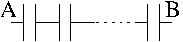
\includegraphics[scale=1.2]{immagini/fisica2/cond2}
\end{figure}
$n$ condensatori sono collegati in serie quando la $\Delta V$ ai capi della combinazione è la somma delle $\Delta V_i$. Siano all'inizio scarichi. Se poniamo una carica $q$ sull'armatura del primo condensatore allora sulla seconda armatura del primo condensatore si crea per induzione una carica opposta $-q$ e sulla prima armatura del secondo condensatore una carica $q$ in modo che la somma della seconda armatura del primo condensatore e la prima del secondo condensatore, che formano un unico conduttore, sia nulla. Se poi l'ultimo condensatore lo colleghiamo a terra avremo che per ogni condensatore si avrà una carica $q$ sulla prima armatura e $-q$ sulla seconda. La carica di ogni condensatore è allora la stessa, quindi la differenza di potenziale di ogni condensatore dipenderà solo dalla propria capacità 
\[\Delta\varphi_i=\frac{q}{C_i}\]
Abbiamo detto che la differenza di potenziale tra i capi $A$ e $B$ è la somma delle differenze di potenziali:
\[\varphi_A-\varphi_B=\sum_{i=1}^N\varphi_i=\sum_{i=1}^N\frac{q}{C_i}=q\sum_{i=1}^N\frac{1}{C_i}\]
Il condensatore equivalente, cioè quello che sostituito al sistema in serie produce gli stessi effetti, è quello con capacità 
\[\frac{1}{C_\text{eq}}=\sum_{i=1}^N\frac{1}{C_i}\]
\subsubsection{Parallelo}
\begin{figure}[htbp]
\centering
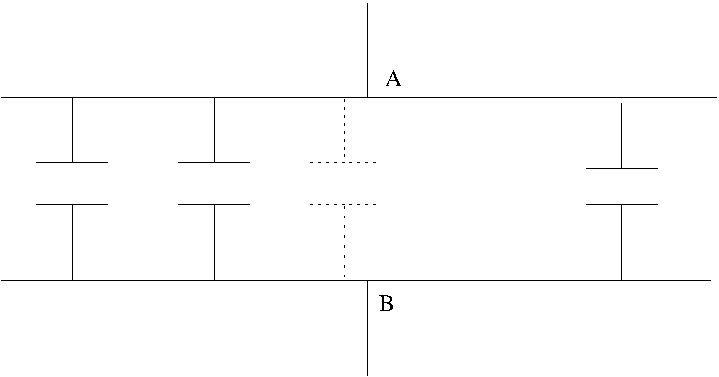
\includegraphics[scale=0.5]{immagini/fisica2/cond3}
\end{figure}
In parallelo la differenza di potenziale di ogni condensatore è uguale. La somma delle cariche è 
\[Q=\sum_{i=1}^N q_i=\sum_{i=1}^N C_i\varphi\]
Allora il condensatore equivalente ha capacità 
\[C_\text{eq}=\sum_{i=1}^N C_i\]

\chapter{Problema generale dell'elettrostatica}
\minitoc
Abbiamo detto che l'elettrostatica è descritta completamente solo da due leggi:
\begin{subequations}
 


\begin{gather}
\ve\nabla\cdot\ve E=\frac{\rho}{\varepsilon_0}
\label{eq:div_E}\\
\ve\nabla\times\ve E=0
\label{eq:rot_E}
\end{gather}
\end{subequations}
Dalla \eqref{eq:rot_E} che ci dice che $\ve E$ è irrotazionale, sappiamo che deve esistere una funzione scalare che è il potenziale di $\ve E$:
\begin{equation}
\ve E=-\ve\nabla\varphi
\label{eq:poisson_pot}
\end{equation}
Sostituendola nella \eqref{eq:div_E}, che non abbiamo ancora usato, otteniamo una singola equazione:
\begin{equation}
\nabla^2\varphi=-\frac{\rho}{\varepsilon_0}
\label{eq:Poisson01}
\end{equation}
Si può anche scrivere:
\[\nabla^2\varphi=\ve\nabla\cdot\ve\nabla\varphi=\diver\grad\varphi={\frac{\partial^2 \varphi}{\partial x^2}+\frac{\partial^2 \varphi}{\partial y^2}+\frac{\partial^2 \varphi}{\partial z^2}}=-\frac{\rho}{\varepsilon_0}\]
L'operatore $\nabla^2$ è il laplaciano\index{laplaciano} e l'equazione differenziale alle derivate parziali \eqref{eq:Poisson01} è l'equazione di Poisson\index{equazione!di Poisson}\index{Poisson}. Risolvere l'equazione di Poisson significa trovare $\varphi(\ve r)$ in funzioni delle condizioni del problema. Dalla conoscenza di $\varphi$: $\ve E=-\ve\nabla\varphi$. L'elettrostatica può essere quindi descritta, oltre che dalle equazioni~\eqref{eq:div_E} e \eqref{eq:rot_E}, dalle equazioni \eqref{eq:Poisson01} e \eqref{eq:poisson_pot}. Il problema così forumulato è ora più semplice, in quanto l'equazione \eqref{eq:poisson_pot} è semplicemente il calcolo di un gradiente, mentre l'equazione \eqref{eq:Poisson01} pur essendo di un ordine superiore all'originale, riguarda una funzione scalare e può essere facilmente generalizzato, per esempio se la sorgente del campo è data esclusivamente da cariche elettriche in un volume allora l'unica soluzione è 
\[\varphi(\ve r)=\frac{1}{4\pi\varepsilon_0}\int_V\frac{\rho(\ve r\,')}{\norm{\ve r-\ve r\,'}}\,\ud v'\]
Il problema diventa più complesso quando si inseriscono dei conduttori che subiscono l'induzione elettrostatica.
\section{Funzioni armoniche}
Se non ci sono cariche, cioè $\rho=0$, allora l'equazione di Poisson diventa:
\begin{equation}
\nabla^2\varphi=0
\label{eq_laplace}
\end{equation}
detta equazione di Laplace\index{equazione!di Laplace}\index{Laplace}. Una funzione che rispetta la \eqref{eq_laplace} e che abbia derivate prime continue è detta armonica\index{funzione!armonica}. Quindi se non ci sono cariche $\varphi$ è armonica. La zona di armonicità di una funzione è l'insieme dei punti dove la funzione è armonica.
\subsection{Teoremi}
Tipicamente i problemi di elettrostatica vengono formulati attraverso le condizioni di Dirichlet o di Neumann. Le prime impogono che la funzione $\varphi$ assuma certi valori su una superficie, le seconde invece impongono condizioni sulle derivate normali (derivata direzionale rispetto alla normale della superficie).
\begin{Teo}[unicità  problema di Dirichlet]
Data una superficie chiusa $S$ la funzione armonica che su $S$ assume il valore $\varphi_S$ è unica.
\end{Teo}
$\varphi_S$ non deve essere necessariamente una costante.
\begin{Teo}[unicità  problema di Neumann]
Siano $\varphi_1$ e $\varphi_2$ due funzioni armoniche definite in un volume tali che le derivate normali siano uguali, allora $\varphi_1$ e $\varphi_2$ differiscono per una costante.
\end{Teo}
\begin{Teo}[media]
Sia $S$ una sfera contenuta in una zona di armonicità di $\varphi$. Allora il valor medio che $\varphi$ assume sulla superficie di $S$ è uguale al valore che $\varphi$ assume nel centro della sfera.
\end{Teo}
\section{Soluzione dell'equazione di Laplace}
Tentiamo di risolvere l'equazione di Laplace, cioè quando non ci sono cariche libere, in casi particolari.
\subsection{Soluzione generale}
\subsubsection{Coordinate cartesiane}
\begin{multline}
\varphi(x,y,z)=\left(A\sin k_x x+B\cos k_x x\right)\left(C\sin k_y y+D\cos k_y y\right)\\\left(Ee^{\sqrt{-k_z^2+k_y^2}z}+Fe^{\sqrt{k_z^2+K_y^2}z}\right)
\end{multline}
\subsubsection{Coordinate cilindriche}
\begin{equation}
\varphi(r,\theta,z)=\left(A\log r+B\right)\left(C\theta+D\right)\left(Ez+F\right)
\end{equation}
\subsubsection{Coordinate sferiche}
\begin{equation}
\varphi(r,\theta,\phi)=\sum_{l,m}\left(E_lr^l+F_lr^{-(l+1)}\right)\left(C_lP_l^m+D_lQ_l^m\right)\left(A\sin m\phi+B\cos m\phi\right)
\end{equation}
\section{Caso monodimensionale}
Supponiamo che il potenziale $\varphi$ dipenda solo dalla coordinata $x$, allora $\frac{\partial\varphi}{\partial y}=\frac{\partial\varphi}{\partial z}=0$ e l'equazione di Laplace diventa:
\[\frac{\ud^2\varphi}{\ud x^2}=0\]
Allora:
\[\frac{\ud \varphi}{\ud x}=a\qquad \varphi=ax+b\]
\begin{Es}[condensatore]
Consideriamo due piani paralleli, tenuti a potenziali $\varphi_1<\varphi_2$, a distanza $d$. Possiamo usare l'equazione di Laplace perché non ci sono cariche libere. Vogliamo il potenziale tra i due piani. Esso dipende solo dalla coordinata $x$ e quindi è un problema monodimensionale. Sia primo piano di equazione $x=0$. La soluzione generale è 
\[\varphi(x)=ax+b\]
Le condizioni al contorno sono:
\[\varphi(0)=\varphi_1\qquad\varphi(d)=\varphi_2\]
Allora:
\[\varphi(x)=\frac{\varphi_2-\varphi_1}{d}x+\varphi_2\]
Il campo:
\[\ve E_E=-\ve\nabla\varphi=\frac{\varphi_1-\varphi_2}{d}\ver \imath\]
Usando il teorema di Coulomb \eqref{eq:teo_coulomb}:
\[\sigma=\varepsilon_0E=\frac{\varphi_1-\varphi_2}{d}\varepsilon_0\]
\end{Es}
\begin{Es}[sfera in condensatore]
Sia una sfera conduttrice di raggio $R$ al centro di un condensatore a facce piane e parallele. Consideriamo un sistema di riferimento centrato nella sfera. Sia $\pm\sigma$ la densità di carica sulle facce a distanza $2d$, allora il campo elettrico esterno, cioè prodotto dal condensatore è 
\[\ve E=\frac{\sigma}{\varepsilon_0}\ver \imath\]
fissiamo il riferimento del potenziale sulla prima armatura che poniamo a terra. Il potenziale esterno:
\[\varphi_{E}(x)=-\frac{\sigma}{\varepsilon_0}(x+d)\]
Usiamo le coordinate polari. Sia $\ve R$ tale che $\norm{\ve R}=R$. Il potenziale esterno sulla superficie del conduttore:
\[\varphi_E(\ve R)=-\frac{\sigma}{\varepsilon_0}\left(R\cos\theta+d\right)\]
Le cariche indotte sulla sfera produrranno un campo e un potenziale indotto che si sommerà 
\[\varphi_T=\varphi_E+\varphi_I\]
Il conduttore è una superficie equipotenziale e quindi $\varphi_T$ deve essere costante.
\[\varphi_T(\ve R)=\varphi_E(\ve R)+\varphi_I(\ve R)=\const\]
\begin{align*}
\varphi_I(\ve R)&=\const-\varphi_E(\ve R)=\const+\frac{\sigma}{\varepsilon_0}(R\cos\theta+d)=\const+\frac{\sigma}{\varepsilon_0}d+\frac{\sigma}{\varepsilon_0}R\cos\theta\\
&=\const+\frac{\sigma}{\varepsilon_0}d+\frac{\sigma}{\varepsilon_0}\ve R\cdot\ver \imath
\end{align*}
e mho?
\end{Es}

\section{Metodo delle cariche immagine}
Il metodo delle cariche immagine è talvolta utile in problemi al bordo, cioè con superfici di tenute ad un potenziale fisso e conosciuto, nei quali siano presenti anche cariche libere. A volte è possibile simulare l'effetto delle superfici con delle cariche opportune posizionate all'esterno del volume di interesse, chiamate cariche immagine.
\begin{Es}[carica e piano infinito]
 \label{es:carica_e_piano_infinito}
 Sia una carica $q$ posizionata sull'asse $x_+$ e sia il piano $y-z$ tenuto a terra. La stessa situzione si realizza con la carica $q$ e una carica immagine $-q$ posizionata simmetricamente rispetto alla carica reale. Infatti il potenziale delle due cariche:
 \[
  \varphi(x,y,z)=\frac{1}{\giorgi}\left(\frac{q}{\sqrt{(x-x_+)^2+y^2+z^2}}+\frac{-q}{\sqrt{(x-x_-)^2+y^2+z^2}}\right)
 \]
e sul piano ($x=0$):
 \[
  \varphi(0,y,z)=\frac{1}{\giorgi}\left(\frac{q}{\sqrt{x_+^2+y^2+z^2}}+\frac{-q}{\sqrt{x_-^2+y^2+z^2}}\right)=0
 \]
in quanto $x_+ = -x_-$. La somma del potenziali delle due cariche è la soluzione per il semispazio di destra ($x>0$). Nel semispazio in cui c'è la carica di prova invece il potenziale è costante, e in questo caso nullo, in quanto il semispazio di sinistra si può considerare come uno spazio interno al conduttore piano infinito. Per determinare la densità di carica sul piano serve la componente normale del campo elettrostatico:
\[
 E_x(0,y,z) = -\frac{\partial\varphi}{\partial x}(0,y,z) = -\frac{q}{2\pi\varepsilon_0}\frac{x_+}{(x_+^2+y^2+z^2)^{3/2}}
\]
quindi usando il teorema di Coulomb \eqref{eq:teo_coulomb}:
\[
 \sigma = \varepsilon_0 E_x = -\frac{qd}{2\pi(d^2+y^2+z^2)^{3/2}}
\]
Integrando su tutto il piano si ottiene:
\begin{equation*}
 \begin{aligned}
  Q &= \int_\text{piano} \sigma\,\ud a = \int -\frac{qd}{2\pi(d^2+y^2+z^2)^{3/2}}\,\ud y\,\ud z\\
    &= -\int \frac{qd}{2\pi(d^2+\rho^2)^{3/2}} \rho\,\ud\rho\sin\theta\,\ud\theta\\
    &= -\frac{2\pi qd}{2\pi}\int_0^\infty \frac{\rho\ud\rho}{(d^2+\rho^2)^{3/2}}\\
    &= -qd\int_{d^2}^\infty \frac{\ud t}{2t^{3/2}} = -q
 \end{aligned}
\end{equation*}
avendo usato la sostituzione $t=\rho^2+d^2$ e il fatto che l'integrando non dipende da $\theta$. Il risultato significa che la carica indotta sulla superficie del conduttore piano è uguale ed opposta alla carica reale, infatti si tratta di induzione completa.
\end{Es}
\begin{Es}[carica e sfera]
 Consideriamo una sfera centrata nell'origine di raggio $a$ a potenziale nullo. Consideriamo una carica puntiforme $q$ a distanza $d$ dall'origine. Supponendo che sia sufficiente una sola carica immagine sicuramente la sua posizione per simmetria sarà sulla congiungente del centro della sfera e la carica reale. In generale il potenziale generato dalle due cariche:
 \begin{equation*}
 \begin{aligned}
  \varphi(\ve x) &= \frac{1}{\giorgi}\left(\frac{q}{\norm{\ve x -\ve d}}+\frac{q'}{\norm{\ve x-\ve d'}}\right)\\
		 &= \frac{1}{\giorgi}\left(\frac{q}{\norm{x\ver n -d\ver n'}}+\frac{q'}{\norm{x\ver n-d'\ver n'}}\right)
 \end{aligned}
 \end{equation*}
 dove $\ver n$ è il versore di $\ve x$ e $\ver n'$ è il versore di $\ve d$ e anche di $\ve d'$. Sulla sfera:
 \begin{equation*}
 \begin{aligned}
  \varphi(x=a) &= \frac{1}{\giorgi}\left(\frac{q}{\norm{a\ver n -d\ver n'}}+\frac{q'}{\norm{a\ver n-d'\ver n'}}\right)\\
	       &= \frac{1}{\giorgi}\left(\frac{q}{a\norm{\ver n -\frac{d}{a}\ver n'}}+\frac{q'}{a\norm{\ver n-\frac{d'}{a}\ver n'}}\right)=0
 \end{aligned}
 \end{equation*}
quindi una soluzione è $d=d'$ e $q=-q'$ ma non va bene, perché $q'$ è all'esterno della sfera. Quindi raccogliendo in modo diverso:
\begin{equation*}
 \begin{aligned}
  \varphi(x=a) &= \frac{1}{\giorgi}\left(\frac{q}{a\norm{\ver n-\frac{d}{a}\ver n'}}+\frac{q'}{d'\norm{\ver n'-\frac{a}{d'}\ver n}}\right)\\
  &= \frac{1}{\giorgi}\left(\frac{q}{a\left(1+\frac{d^2}{a^2}-2\frac{d}{a}\ver n\cdot\ver n'\right)^{1/2}}+\frac{q'}{d'\left(1+\frac{a^2}{d'^2}-2\frac{a}{d'}\ver n\cdot\ver n'\right)^{1/2}}\right)
  \end{aligned}
\end{equation*}
e deve essere:
\[
 \frac{q}{a}=-\frac{q'}{d'}\qquad \frac{d}{a}=\frac{a}{d'}
\]
in modo che il potenziale si annulli sulla sfera per ogni possibile valore di $\ver n\cdot\ver n'$.  Quindi per la carica immagine:
\[
 q'=\frac{-a}{d}q\qquad d'=\frac{a^2}{d}
\]
In questo caso la carica immagine è all'interno della sfera, in quando $a < d\Rightarrow d'<a$. Quindi il potenziale:
\[
 \varphi(\ve x) = \frac{1}{\giorgi}\left(\frac{q}{\norm{x\ver n -d\ver n'}}+\frac{-\frac{a}{d}q}{\norm{x\ver n-\frac{a^2}{d}\ver n'}}\right)
\]
\begin{figure}[htbp]
 \centering
 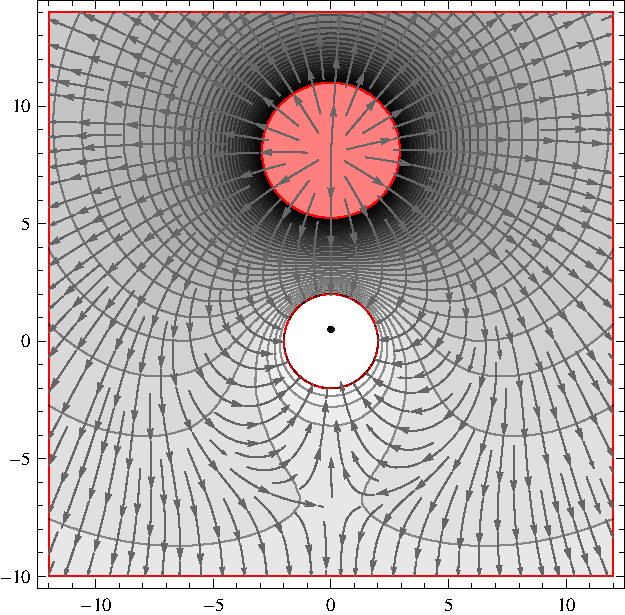
\includegraphics{immagini/fisica2/sfera_neutra}
 \caption{Linee equipotenziali e linee di campo nel piano $y=0$. Le linee rosse indicano le regioni dove non è stato calcolato il potenziale. La sfera ha raggio $2$, mentre la carica unitaria positiva è in $(0,8)$. Il punto indica la posizione della carica immagine.}
\end{figure}
\end{Es}
\begin{Es}[sfera in campo uniforme]
\begin{figure}[htbp]
 \centering
 \begin{tikzpicture}[scale=1]
\coordinate (O) at (0,0);
\coordinate (q) at (0.5,0);
\coordinate (-q) at (-0.5,0);
\coordinate (p) at (xyz polar cs:angle=25, radius=3.5);
\draw[->] (-6,0) -- (6,0) node[above] {$z$};
\draw[->] (0,-2) -- (0,2);
\draw (O) circle (1.5cm);
\draw[<->] (O) -- (xyz polar cs:angle=250, radius=1.5) node[near end,sloped,above]{$a$};
\filldraw[black] (4.5,0) circle(2pt) node[below right]{$-Q$};
\draw[->,shorten >=2pt] (O) -- (4.5,0) node[near end,above]{$\ve R_-$};
\filldraw[black] (-4.5,0) circle(2pt) node[below left]{$+Q$};
\draw[->,shorten >=2pt] (O) -- (-4.5,0) node[near end,above]{$\ve R_+$};
\filldraw[black] (-q) circle(2pt) node[below left]{$-q$};
\filldraw[black] (q) circle(2pt) node[below right]{$+q$};
\draw (2,0) arc (0:25:2.0cm) node[below right]{$\theta$};
\draw[->,shorten >=2pt] (O) -- (p) node[midway, above]{$\ve r$};
\filldraw[black] (p) circle(2pt) node[above
  right]{$P$};
\draw[dotted] (-q) -- (-0.5,0.8);
\draw[<->] (-0.5,0.8) -- (0,0.8) node[midway,above]{$d'$};
\end{tikzpicture}%

 \caption{La sfera a potenziale nullo può essere sostituita da due cariche immagine al suo interno.}
 \label{fig:esempio_campo_sfera}
\end{figure}

 Consideriamo un campo uniforme di modulo $E_0$ diretto come l'asse $z$ e una sfera conduttrice centrata nell'origine, di raggio $a$ messa a terra. Il campo uniforme può essere simulato da due cariche puntiformi poste all'infinito in direzioni opposte di carica opposta (vedi fig.~\ref{fig:esempio_campo_sfera}). Infatti il potenziale:
 \[
  \begin{aligned}
   \varphi(\ve r)=&\frac{1}{\giorgi}\frac{Q}{\norm{\ve r - \ve R_+}}+\frac{1}{\giorgi}\frac{-Q}{\norm{\ve r-\ve R_-}}\\
  =&\frac{Q}{\giorgi}\left\{\frac{1}{(r^2+R^2_+-2\ve r\cdot \ve R_+)^{1/2}}-\frac{1}{(r^2+R_-^2-2\ve r\cdot\ve R_-)^{1/2}}\right\}\\
  =&\frac{Q}{\giorgi}\frac{1}{R}\left\{\frac{1}{(\frac{r^2}{R^2}+1+2\frac{r}{R}\cos\theta)^{1/2}}-\frac{1}{(\frac{r^2}{R^2}+1-2\frac{r}{R}\cos\theta)^{1/2}}\right\}
  \end{aligned}
 \]
 si noti che l'angolo tra $\ve R_-$ e $\ve r$ è $\theta$, mentre l'angolo tra $\ve R_+$ e $\ve r$ è $\pi-\theta$. Usando il solito sviluppo usanto anche per lo sviluppo in multipoli:
 \[
  \begin{aligned}
  \left(1+\frac{r^2}{R^2}\pm\frac{2r}{R}\cos\theta\right)^{-1/2}&=1-\frac{1}{2}\left(\frac{r^2}{R^2}\pm\frac{2r}{R}\cos\theta\right)+o\left(\frac{r^2}{R^2}\pm\frac{2r}{R}\cos\theta\right)\\
  &=1\mp\frac{r}{R}\cos\theta+o\left(\frac{r}{R}\right)
  \end{aligned}
 \]
 quindi l'approssimazione per $R\to\infty$:
 \[
  \varphi(\ve r)=-\frac{1}{\giorgi}\frac{2Q}{R^2}\underbrace{r\cos\theta}_z=-\frac{1}{\giorgi}\frac{2Q}{R^2}z
 \]
 sempre che il rapporto $\frac{Q}{R^2}$ rimanga finito. Il campo elettrico è nullo in tutte le componenti tranne:
 \[
  E_z = \frac{1}{\giorgi}\frac{2Q}{R^2}
 \]
 poiché $E_z=E_0$ si ricava che $\frac{2Q}{R^2} = \giorgi E_0$.
 
 Ora bisogna aggiungere delle cariche immagine in modo tale che sulla supreficie della sfera il potenziale risulti nullo. Le due cariche dovranno essere all'interno della sfera. Per simmetria dovranno essere sull'asse $z$, poste in maniera simmetrica. Si può usare l'esempio precedente per ricavare il loro valore e la loro posizione. Consideriamo, grazie al principio di sovrapposizione separatamente la carica $Q$ e la carica $-Q$. Se abbiamo solo la carica $Q$ ci servirà una carica immagine di valore $-\frac{a}{R}Q$ e posta a $d'=\frac{a^2}{R}$ (vedi esercizio precedente). Discorso analogo per la carica $-Q$. Quindi il potenziale generato dalle quattro cariche risulta:
 \[
  \begin{aligned}
   \varphi(\ve r)=\frac{Q}{\giorgi}\Biggl\{\frac{1}{(r^2+R^2+2rR\cos\theta)^{1/2}}-\frac{1}{(r^2+R-2rR\cos\theta)^{1/2}}-\\
   -\frac{\frac{a}{R}}{(r^2+d'^2+2d' r\cos\theta)^{1/2}}+\frac{\frac{a}{R}}{(r^2+d'^2-2d' r\cos\theta)^{1/2}}\Biggr\}
  \end{aligned}
 \]
 i primi due termini sono quelli di prima. Ora per fare $R\to\infty$ gli ultimi due termini si espandono in maniera analoga:
 \[
  \left(r^2+\frac{a^4}{R^2}\pm 2\frac{a^2}{R}r\cos\theta\right)^{-1/2} = r^{-1}\left(1\mp\frac{a^2}{Rr}\cos\theta+o\left(\frac{a^2}{Rr}\right)\right)
 \]
 mettendo tutto insieme:
 \[
  \varphi(\ve r) = \frac{Q}{\giorgi}\left\{\frac{2}{R^2}r\cos\theta+\frac{2a^3}{R^2r^2}\cos\theta\right\}
 \]
 si noti che la coppia di cariche all'interno della sfera costituisce un dipolo $\ve p = q(2d')\ver z$, infatti con la teoria del dipolo per $R\to\infty$ ($d'\to 0$):
 \[
  \varphi_\text{dipolo}(\ve r) = \frac{1}{\giorgi}\frac{\ve p\cdot\ve r}{r^3} = \frac{q}{\giorgi}\frac{2d'z}{r^3} = \frac{\frac{a}{R}Q}{\giorgi}\frac{2\frac{a^2}{R}z}{r^3}=\frac{Q}{\giorgi}\frac{2a^3}{R^2r^2}\cos\theta
 \]
 Infine considerando che $\frac{2Q}{R^2} = \giorgi E_0$ (cioè $p=\giorgi E_0 a^3$):
 \[
  \varphi(\ve r)=-E_0\left(r-\frac{a^3}{r^2}\right)\cos\theta
 \]
 \begin{figure}[htbp]
 \centering
 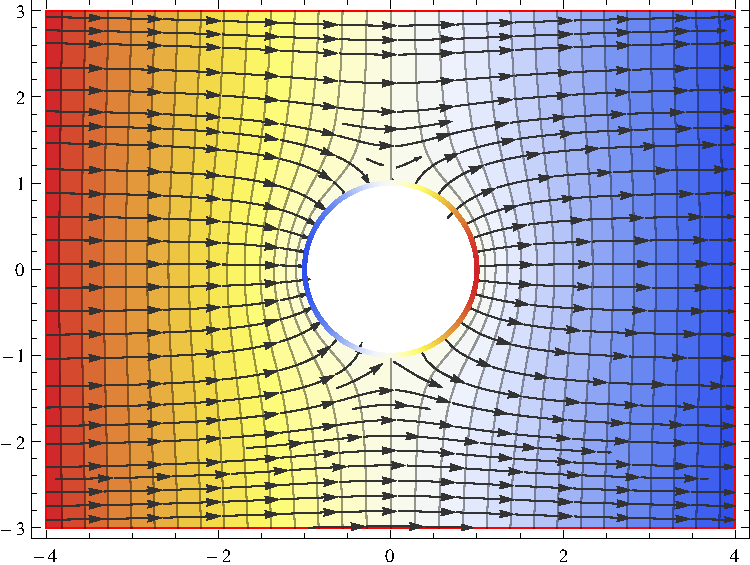
\includegraphics[scale=1]{immagini/fisica2/campo_con_sfera}
 \caption{Linee equipotenziali e linee di campo per una sfera a potenziale nullo immersa in un campo elettrostatico uniforme. Il colore sul bordo della sfera indica la carica superficiale.}
\end{figure}
 Si può ricavare la densità di carica dal teorema di Coulomb:
 \[
  \sigma = \varepsilon_0\ve E\cdot \ver n = -\varepsilon_0\left.\frac{\partial\varphi}{\partial r}\right|_{r=a}=3\varepsilon_0 E_0\cos\theta
 \]
 Quindi la carica totale indotta sulla sfera:
 \[
  Q = \int \sigma\,\ud a = \int_0^\pi 3\varepsilon_0 E_0\cos\theta 2\pi a\sin\theta a\,\ud\theta = 3\varepsilon_0E_02\pi a^2\int_0^\pi\sin\theta\cos\theta = 0
 \]
 quindi si può concludere che in questo caso non c'è differenza tra una sfera a terra e una sfera isolata.
 
 All'interno il campo è nullo, quindi il campo generato dalla carica indotta sulla sfera deve essere uguale ed opposto al campo esterno. Abbiamo quindi anche dimostrato che una sfera carica con una densità di carica che varia come $\cos\theta$ genera un campo interno uniforme e un campo esterno di dipolo. Dal segno della densità di carica si deduce la discontinuità che deve avere il campo elettrico e quindi che il campo elettrico interno costante è diretto dall'emisfero dove $\cos\theta>0$ all'emisfero dove $\cos\theta<0$.
\end{Es}


\chapter{Corrente stazionaria\index{corrente!stazionaria}}
\minitoc
Per definizione la corrente è un flusso ordinato di cariche elettriche, la grandezza che la caratterizza è l'intensità di corrente:
\begin{Def}[intensità di corrente\index{intensità di corrente}]
\begin{equation}
I=\frac{\ud q}{\ud t}
\label{corrente_def}
\end{equation}
\end{Def}
\`E una grandezza scalare, anche se la corrente ha un verso, quello del moto delle cariche positive e una direzione, quella del campo elettrico. Per corrente stazionaria si intende una corrente che è costante nel tempo. La corrente non ha bisogno della presenza di un conduttore. Si misura in ampere (\ampere): \coulomb\per\second \footnote{in realtà è il Coulomb che dovrebbe essere definito come Ampere secondo, vedi oltre per definizione di ampere}. Dall'equazione \eqref{corrente_def}:
\begin{equation}
Q=\int_0^t I(t')\ud t'
\end{equation}
essendo però la corrente stazionaria $Q=It$. Il moto delle cariche ha origine da una differenza di energia potenziale e quindi da una differenza di potenziale. Tutte le particelle cariche che con il loro moto generato una corrente si chiamano portatori di cariche. Muovendo un corpo carico, per esempio traslandolo, si crea una corrente, in quanto si stanno muovendo delle cariche; per differenziare queste correnti non del tutto proprie, chiameremo correnti di conduzione il moto di portatori di carica all'interno del corpo, senza movimento del corpo.
\section{Modello del gas di elettroni liberi\index{modello del gas di elettroni liberi}}
Ipotizziamo che gli elettroni liberi si muovano come gli atomi di un gas classico, quindi con urti casuali, ecc\ldots
In assenza di campo elettrico gli elettroni saranno in agitazione termica con una velocità $v_T$ di agitazione termica:
\[K=\frac{1}{2}m_{\mathrm{e}}v_T^2=\frac{f}{2}kT\]
con $f=3$ gradi di libertà  $k$ costante di Boltzmann. Alla temperatura di $\si{300}{\kelvin}$:
\[v_T=\sqrt{\frac{3kT}{m}}\simeq \SI{1E5}{\metre\per\second}\]
Definiamo $\tau$ il tempo medio tra due urti consecutivi e $l$ il libero cammino medio, cioè lo spazio medio che un elettrone percorre senza urti:
\[l = \tau v_T\]
Se ora applichiamo un campo elettrico $\ve E$ costante, provocheremo un altro moto dovuto alla forza elettrica con velocità $v_D$, velocità di deriva\index{velocità!di deriva}, che bisogna sovrapporre a quello di agitazione termica. A temperature usuali $v_D\ll v_T$ e quindi $\tau$ e $l$ rimangono pressoché invariati.
\section{Densità di corrente}
Consideriamo un conduttore con $N$ portatori di carica per unità di volume, tutti uguali, con carica $q$ e velocità di deriva $v_D$. Nel tempo $\ud t$ attraverso una sezione $\ud A$ passa una quantità di carica:
\begin{equation}
\frac{\ud Q}{\ud t}=\ud I=qN\left(\ve v_D\cdot \ve n\right)\ud a
\label{densita_corrente01}
\end{equation}
\begin{Def}[densità di corrente\index{densità di corrente}]
Si definisce $\ve J$ densità di corrente:
\begin{equation}
\ve J=qN\ve v_D
\end{equation}
\end{Def}
Allora la \eqref{densita_corrente01} si scrive come:
\[\ud I=\ve J\cdot\ve n\,\ud a\]
E la corrente totale:
\begin{equation}
I=\int_S \ve J\cdot \ve n\,\ud a
\end{equation}
che è l'espressione di un flusso, precisamente il flusso di $\ve J$:
\begin{equation}
I=\Phi_S\left(\ve J\right)
\end{equation}
\subsection{Conservazione della carica\index{conservazione!della carica}}
Applicando il teorema della divergenza:
\begin{equation}
I=\int_S \ve J\cdot\ve n\,\ud a=-\int_V\ve\nabla\cdot\ve J\,\ud V
\label{densita_corrente02}
\end{equation}
il segno meno è dovuto al fatto che consideriamo positive le correnti che entrano nel volume $V$. Per definizione di corrente:
\begin{equation}
I=\frac{\ud Q}{\ud t}=\frac{\ud}{\ud t}\int_V\rho\,\ud V
\label{densita_corrente03}
\end{equation}
Confrontando la \eqref{densita_corrente02} e la \eqref{densita_corrente03} si ottiene:
\[\int_V\frac{\partial \rho}{\partial t}=-\int_V\ve\nabla\cdot\ve J\,\ud V\]
per l'arbitrarietà di $V$:
\begin{legge}[conservazione della carica\index{conservazione!della carica}]
\begin{equation}
\diver\ve J=-\frac{\partial \rho}{\partial t}
\end{equation}
\label{conservazione della carica}
\end{legge}
la legge \eqref{conservazione della carica} è detta anche principio di continuità \index{principio! di continuità}. Le sorgenti del campo $\ve J$ sono le variazioni di densità di carica. In condizioni stazionarie $\frac{\partial\rho}{\partial t}=0$ e dunque:
\[\diver \ve J=0\]
e dunque $\ve J$ è un campo solenoidale, non ha sorgenti.
\section{Conducibilità elettrica\index{conducibilità elettrica}}
Indichiamo con $N(t)$ il numero di elettroni che al tempo $t$ non hanno subito nessuna collisione. Sia $N_0$ il numero totale di elettroni, ovviamente $N(0)=N_0$. La probabilità media che un elettrone subisca un urto nel tempo $\ud t$ è $\frac{\ud t}{\tau}$. Quindi in media il numero di elettroni che subiscono un urto nel tempo $\ud t$ è $N_0(t)\frac{\ud t}{\tau}$. Il numero di elettroni che subiscono il primo urto $N(t)\frac{\ud t}{\tau}$. Allora:
\[N(t+\ud t)=N(t)-N(t)\frac{\ud t}{\tau}\]
Facendo il primo sviluppo di Taylor:
\[N(t+\ud t)=N(t)+\frac{\ud N}{\ud t}\ud t\]
Confrontando:
\[\ud N(t)=-N(t)\frac{\ud t}{\tau}\]
che rappresenta il numero di elettroni che hanno subito un urto nell'intervallo $\ud t$ dopo il tempo $t$.
\[\frac{\ud N}{N}=-\frac{\ud t}{\tau}\ud t\]
Risolvendo:
\[\log N(t)=-\frac{t}{\tau}+c \qquad N(t)=e^{-\frac{t}{\tau}+c}=Ae^{-\frac{t}{\tau}}\]
Imponendo che $N(0)=N_0$:
\[N(t)=N_0e^{-\frac{t}{\tau}}\]
Il numero di elettroni che non hanno subito una collisione decresce molto rapidamente. La probabilità che al tempo $t$ un elettrone non abbia subito collisioni è
\[P(t)=\frac{N(t)}{N_0}=e^{\frac{-t}{\tau}}\]
Vogliamo ora sapere quanto tempo ci vuole ad avere un urto qualsiasi dopo il tempo $t$:
\[\overline{t}=\frac{1}{N_0}\int_0^\infty t\frac{N(t)}{\tau}\,\ud t=\frac{1}{N_0}\int_0^\infty\frac{tN_0 e^{-\frac{t}{\tau}}}{\tau}\ud t=\frac{1}{\tau}\int_0^\infty te^{-\frac{t}{\tau}}=\tau\]
Quindi $\tau$ non è solo il tempo medio tra un urto di una particella e il successivo, sempre di quella particella, ma è anche il tempo medio che al tempo $t$ bisogna attendere per avere il primo urto tra due particelle qualsiasi. Naturalmente essendo indipendente dal tempo $\tau$ è anche il tempo medio dall'ultimo urto. Possiamo calcolare la velocità di deriva, considerando l'accelerazione data dal campo elettrico durante il tempo dall'ultimo urto:
\[\ve v_D=\ve a\tau=\frac{\ve F}{m_\mathrm{e}}=\frac{-e}{m_\mathrm{e}}{\ve E}\tau\]
Usando la densità di corrente:
\[\ve J=-Ne\ve v_D=\frac{e^2\tau N}{m_\mathrm{e}}\ve E=\sigma\ve E\]
$\sigma$ è la conducibilità elettrica:
\[\sigma=\frac{e^2\tau N}{m_\mathrm{e}}=\frac{e^2Nl}{m_\mathrm{e}v_D}\]
La conducibilità elettrica ci dice come il conduttore risponde al campo elettrico, l'ostacolo che gli elettroni incontrano nel loro moto; alta conducibilità significa alta disposizione da parte del conduttore di mettere in moto i suoi elettroni. Se supponiamo che $\sigma$ non dipenda dallo spazio, cioè il conduttore sia omogeneo, che $\sigma$ non dipenda da $E$, cioè che il conduttore sia lineare e che non dipenda dalla direzione di $\ve E$ cioè sia isotropo e quindi $\ve J$ abbia la direzione di $\ve E$ allora $\sigma$ è uno scalare, altrimenti è un tensore $3\times 3$ del second'ordine:
\[\ve J=\ten{\sigma}\ve E\]
\subsection{Resistività \index{resistività}}
\begin{Def}[resistività elettrica]
La resistività $\rho$ è l'inverso della conducibilità 
\[\rho=\frac{1}{\sigma}\]
\end{Def}
Più la resistività è alta più la risposta al campo elettrico del conduttore sarà bassa.
\subsection{Unità di misura}
\[[\sigma]=\frac{[J]}{[E]}=\frac{\ampere}{\metre\squared}\frac{\metre}{\volt}=\si{}{\per\ohm\per\metre}\]
\[[\rho]=\ohm\meter\]
con:
\[\ohm=\frac{\volt}{\ampere}=\text{ohm}\]
\[\text{ohm}^{-1}=\text{mho}=\mho=\siemens=\text{siemens}\]
\index{ohm}\index{mho}\index{siemens}
\section{Legge di Ohm\index{legge!di Ohm}}
\begin{figure}[htbp]
 \centering
 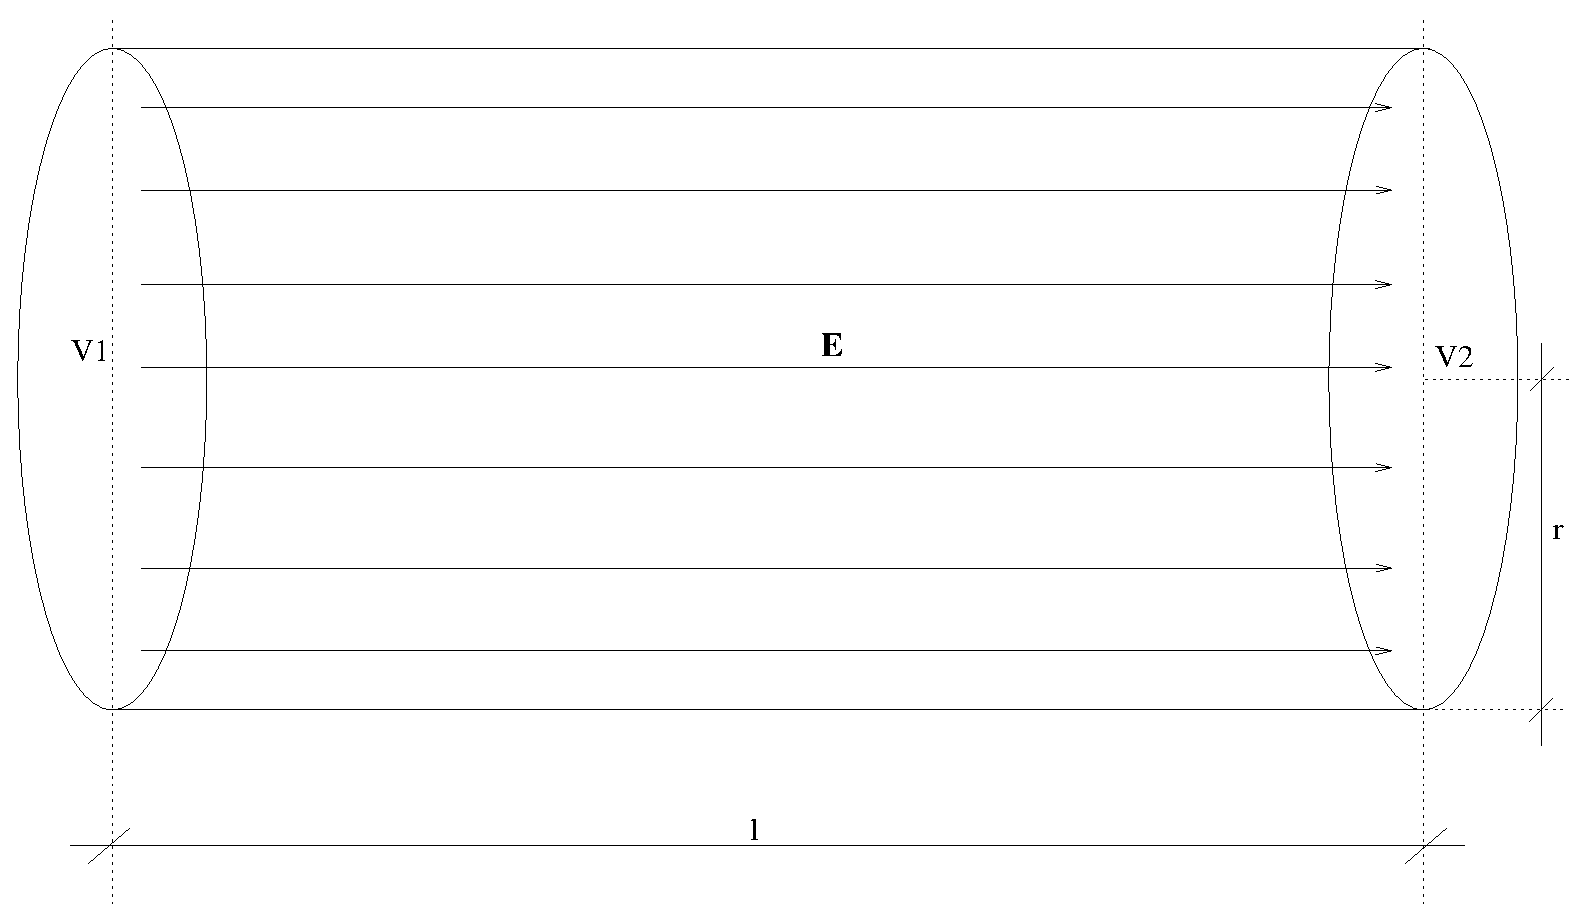
\includegraphics[scale=0.4]{immagini/fisica2/ohm1}
\end{figure}
Consideriamo un filo isotropo, omogeneo, di lunghezza $l$ e sezione $\Sigma$ variabile e con conduttività $\sigma$. Sia $\Delta V$ la differenza di potenziale mantenuta tra i due capi, con $V_1>V_2$. Consideriamo la differenza di potenziale tra due porzioni di superfici equipotenziali:
\begin{equation}
 \ud V = \ve E\cdot\ud \ve l = \frac{\ve J}{\sigma}\cdot\ud\ve l=\frac{\ve J}{\sigma}\cdot\ver n\,\ud l
\end{equation}
dove $\ver n$ è la normale alla superficie. Se integriamo sulla superficie:
\begin{equation}
 \int\ud V\,\ud\Sigma=\int\frac{\ve J}{\sigma}\cdot\ver n\,\ud l\,\ud\Sigma
\end{equation}
poiché la superficie su cui stiamo integrando è equipotenziale $\ud V$ è costante su tutta la superficie e può uscire dall'integrale:
\begin{equation}
 \ud V\int\ud\Sigma = \ud V\Sigma=\frac{\left[\int\ve J\cdot\ud\ve \Sigma\right]\ud l}{\sigma}
\end{equation}
e si è supposto che $\sigma$ sia anch'essa costante su tutta la superficie. Integrando su tutta la lunghezza del conduttore:
\begin{equation}
 \Delta V = \int\ud V=\int\frac{I\ud l}{\Sigma\sigma}
\end{equation}
Essendo gli elementini in serie la corrente è la stessa per tutti, mentre la sezione e la conducibilità potrebbero dipendere dalla posizione: $\sigma=\sigma(l)$, $\Sigma=\Sigma(l)$:
\begin{equation}
 \Delta V = I\int \frac{\ud l}{\Sigma\sigma}=IR
\end{equation}
\begin{Def}[resistenza elettrica\index{resistenza!elettrica}]
 \begin{equation}R=\int_A^B \frac{\rho}{\Sigma}\,\ud l\end{equation}
\end{Def}
\begin{legge}[Ohm]
 \begin{equation}
  \Delta V=IR
 \end{equation}
 \end{legge}
che in realtà è stata introdotta come legge sperimentale. I materiali che rispettano questa legge sono detti ohmnici.\index{materiale ohmnico}
\begin{Es}[Filo]
 Un filo a sezione $S$, resistività $\rho$ entrambi costanti e lunghezza $L$, avrà resistenza:
\begin{equation}
 R=\int_A^B \frac{\rho}{\Sigma}\ud l=\rho\frac{L}{S}
\end{equation}
\begin{figure}[htbp]
 \centering
 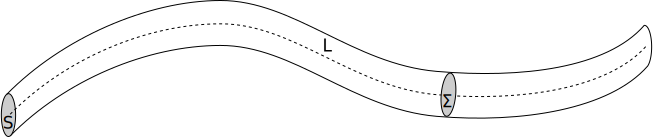
\includegraphics[scale=0.5]{immagini/fisica2/filo_serpente}
 % filo_serpente.pdf: 0x0 pixel, 0dpi, nanxnan cm, bb=
\end{figure}
\end{Es}
\begin{Es}[Conduttori cilindrici]
\begin{figure}[htbp]
 \centering
 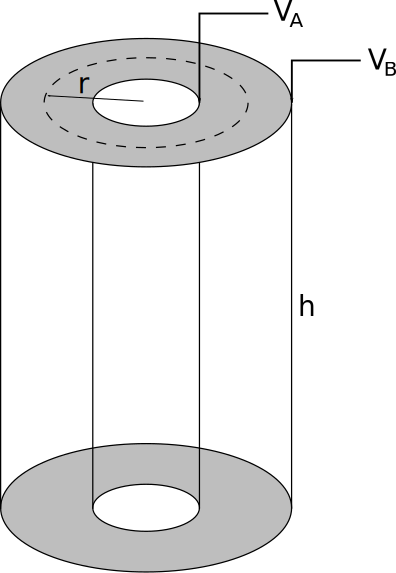
\includegraphics[scale=0.35]{immagini/fisica2/conduttore_cilindrico}
 % conduttore_cilindrico.pdf: 317x458 pixel, 72dpi, 11.18x16.16 cm, bb=0 0 317 458
\end{figure}
 Consideriamo due superfici cilindriche concentriche, e tra queste inseriamo un materiale con resistività $\rho$ uniforme. Appichiamo una $\Delta V$ sulle due superfici, vogliamo sapere quanto è la corrente che scorre.
\[
 R = \frac{\Delta V}{I} = \rho\int\frac{\ud l}{\Sigma(l)}
\]
dove $l$ è la distanza tra un conduttore e l'altro, quindi il raggio. Per la geometria dei conduttori
\[
 \Sigma(r) = 2\pi rh
\]
\[
 R = \rho\int\frac{\ud r}{2\pi rh}=\frac{\rho}{2\pi h}\log\left(\frac{r_B}{r_A}\right)
\]
\[
 I = \frac{\Delta V}{R} = \Delta V \frac{2\pi h}{\rho\log\frac{r_B}{r_A}}
\]
\end{Es}


\subsection{Temperatura}
La temperatura modifica $\rho$ in quanto al crescere della temperatura i nuclei degli elettroni si muovono più velocemente e gli urti con gli elettroni diventano più probabili. L'aumento di resistività del tipo:
\[\rho(T)=\rho_0\left[1+a\left(T-T_0\right)+b\left(T-T_0\right)^2+c\left(T-T_0\right)^3+\cdots\right]\]
di solito $a>b>c>\cdots$ e si considera solo il primo termine:
\[\rho(T)=\rho_0\left(1+\alpha\left(T-T_0\right)\right)\]
considerandolo come uno sviluppo di Taylor:
\[\alpha=\frac{1}{\rho_0}\left.\frac{\partial \rho}{\partial T}\right|_{T_0}\]
Per i semiconduttori \index{semiconduttori} $\alpha<0$. Ad una certa temperatura, detta temperatura critica\index{temperatura!critica}, la resistività crolla e si ha il fenomeno della superconduttività\index{superconduttività}\index{superconduttori}.

Il modello basato sul gas di elettroni non riesce a spiegare questo andamento, infatti:
\[v_T=\sqrt{3\frac{kT}{m_\mathrm{e}}}\]
cioè $\rho\propto v_T\propto\sqrt{T}$ invece che $\rho\propto T$. Inoltre non riesce a spiegare la diversità di $\rho$ tra i diversi materiali, sia conduttori che non, infatti
\[\rho=\frac{m_\mathrm{e}}{e^2N\tau}=\frac{m_\mathrm{e}}{eN}\frac{v_T}{l}\]
dice solo che la variazione tra i diversi materiali è data da $N$, che in realtà non varia di molto da conduttore a conduttore. Nella realtà $\rho$ è influenzato da numerosi fattori tra cui le impurezze cioè il disordine del reticolo.

\subsection{Resistori}
\begin{Def}[resistore\index{resistore}]
Un resistore è un conduttore caratterizzato dal valore della resistenza\footnote{La resistenza è una grandezza, non è un conduttore}.
\end{Def}
\begin{Def}[rete resistiva\index{rete!resistiva}]
Una rete resistiva è un insieme di resistori collegati insieme.
\end{Def}
\begin{Def}[circuito elettrico\index{circuito!elettrico}]
Un circuito è una successione chiusa di resistori e generatori di forza elettromotrice, più eventuali altri elementi.
\end{Def}
\subsubsection{Resistori in serie e in parallelo}
\paragraph{Serie\index{resistori!in serie}}
I resistori si dicono collegati in serie quando sono attraversati tutti dalla stessa corrente. Applicando la legge di Ohm:
\[V_1-V_2=IR_1\qquad \cdots \qquad V_{n-1}-V_{n}=IR_n\]
Sommando tutte le espressioni si ottiene che la caduta di tensione ai capi della rete è 
\[V_1-V_n=I\sum_{i=1}^N R_i\]
Quindi la resistenza equivalente, la resistenza di quel resistore che produce gli stessi effetti dei resistori in serie, è la somma delle resistenze.
\paragraph{Parallelo\index{resistori!in parallelo}}
I resistori si dicono collegai in parallelo quando ai capi di ogni resistore è applicata la stessa differenza di potenziale. Applicando ancora la legge di Ohm:
\[\frac{V_1-V_2}{R_1}\qquad\cdots\qquad\frac{V_1-V_2}{R_n}=I_n\]
Sommando si ottiene che il reciproco del resistore equivalente è la somma dei reciproci dei resistori in parallelo.
\begin{Es}[resistenza corpo esteso]
\begin{figure}[htbp]
\centering
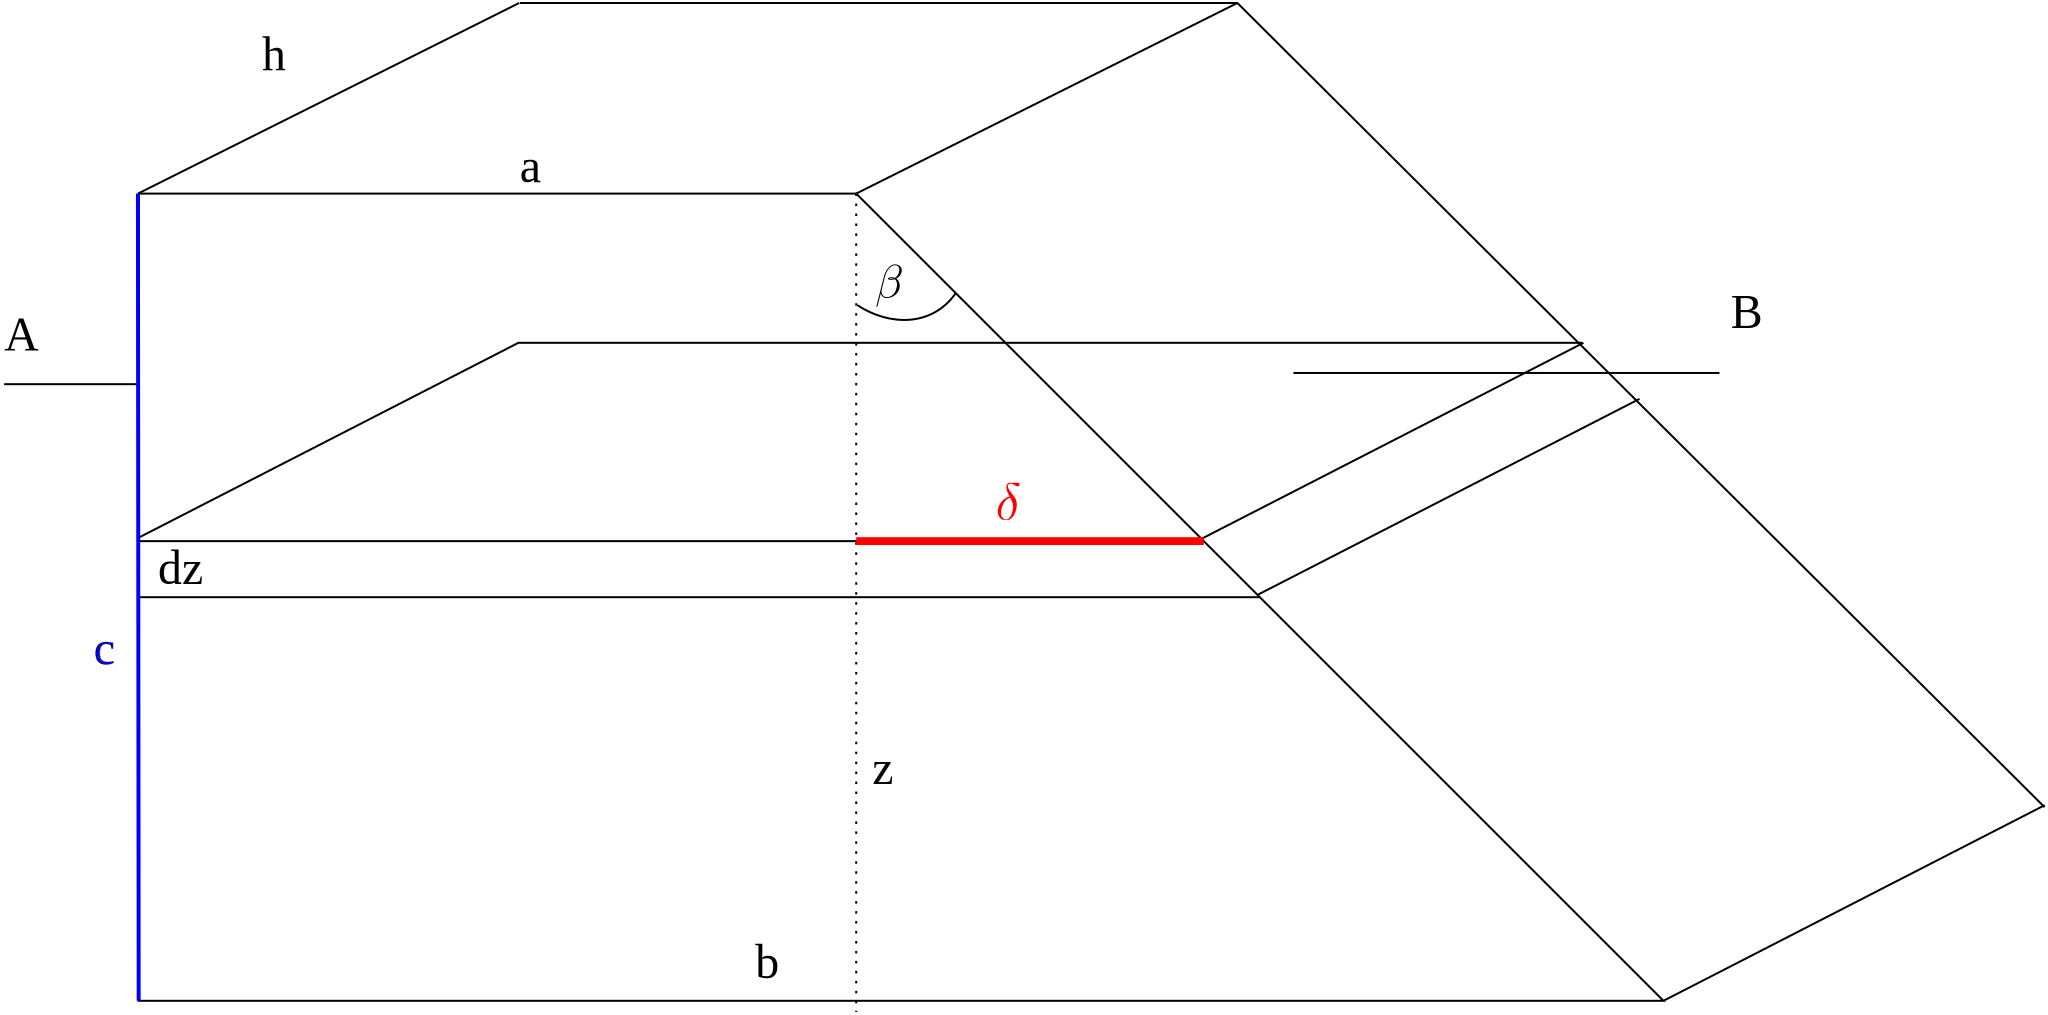
\includegraphics[scale=0.5]{immagini/fisica2/res_trapezio}
\caption{resistenza di un corpo esteso.}
\label{res_trapezio}
\end{figure}
Consideriamo il corpo in figura \eqref{res_trapezio}. Vogliamo calcolare la resistenza tra i capi $A$ e $B$. Scomponiamo la geometria in tanti elementini di altezza $\ud z$, essi risultano in parallelo. La loro resistenza:
\[\ud R=\rho\frac{l}{A}=\rho\frac{y}{h\ud z}\]
con $y=a+\delta$ che varia tra $a$ e $b$. Troviamo $\delta$:
\[
(c-z)\tan\beta=\delta\qquad c\tan\beta=b-a\qquad \delta=(c-z)\frac{b-a}{c}
\]
Allora $y$:
\[y=a+\delta=a+\frac{(c-z)(b-a)}{c}=b+\frac{z}{c}(a-b)\qquad\ud y=\frac{a-b}{c}\ud z\]
\[\frac{1}{R}=\int_0^c\frac{1}{\ud R}=\int_0^c\frac{h\ud z}{\rho y}=\frac{hc}{\rho(a-b)}\int_b^a\frac{\ud y}{y}=\frac{hc}{\rho(a-b)}\log\frac{a}{b}\]
\[R=\frac{\rho(a-b)}{hc\log\frac{a}{b}}\]


\end{Es}


\section{Tempo di rilassamento\index{tempo!di rilassamento!di un conduttore}}
Vogliamo sapere quanto è il tempo necessario per un conduttore per eliminare un eccesso di carica. Consideriamo un conduttore isotropo, omogeneo, lineare, con conducibilità $\sigma$, con un eccesso di carica al tempo zero $\rho_0(\ve r)$ in una regione limitata di spazio. Si creerà un campo elettrico e quindi una densità di corrente $\ve J=\sigma\ve E$. Vogliamo studiare l'evolversi di $\rho(\ve r,t)$. Sappiamo:
\[\diver\ve E=\frac{\rho(\ve r,t)}{\varepsilon_0}\qquad\diver\ve J=-\frac{\partial\rho(\ve r,t)}{\partial t}\]
Essendo $\ve J=\sigma\ve E$:
\[\sigma\diver\ve E=-\frac{\partial\rho}{\partial t}\]
Sostituendo:
\[\frac{\sigma}{\varepsilon_0}\rho=-\frac{\partial\rho}{\partial t}\]
Risolvendo:
\[\frac{\ud\rho}{\rho}=-\frac{\sigma}{\varepsilon_0}\ud t\qquad \log\rho=-\frac{\sigma}{\varepsilon_0}t+c\qquad \rho=Ae^{-\frac{\sigma}{\varepsilon_0}t}=\rho_0 e^{-\frac{\sigma}{\varepsilon_0}t}\]
Chiamando $\tau=\frac{\sigma}{\varepsilon_0}$ tempo caratteristico, o tempo di rilassamento:
\[\rho=\rho_0e^{-\tau t}\]
Il tempo caratteristico \index{tempo!caratteristico} è quel tempo dopo il quale la densità di carica si è ridotta di $\frac{1}{e}$. Dopo qualche $\tau$ possiamo considerare tutto l'eccesso di carica eliminato.

\section{Generatori\index{generatori}}
Con un campo elettrostatico si possono creare correnti, come visto nel paragrafo precedente, ma non mantenerle in quanto il fenomeno si esaurisce in pochissimo tempo. I generatori possono mantenere una differenza di potenziale costate tra i poli o morsetti o variarla secondo una funzione, tipicamente sinusoidale. Nel primo caso si parla di pile\index{pila} o batterie\index{batteria}. In un circuito chiuso:
\[\oint_C\ve E\cdot\ud\ve l=0\]
Essendo $\ve J=\sigma \ve E$:
\[\oint_C\ve J\cdot\ud\ve l=\sigma\oint_C\ve E\cdot\ud\ve l=0\]
\`E assurdo perché non ci sarebbe corrente. Dobbiamo supporre ci siano alte forze, non conservative, che non sono svolte dal campo elettrostatico, essendo il suo lavoro nullo. Tali forze sono localizzate nel generatore. Consideriamo allora un a altro campo $E_i$, il campo elettrico impresso \index{campo!elettrico!impresso}o elettromotore \index{campo!elettromotore}che si somma al campo elettrostatico:
\[\ve E_T=\ve E+\ve E_i\qquad \ve J=\sigma(\ve E+\ve E_i)\]
Il campo impresso nasce quando si è in presenza di una disomogeneità  come ad esempio all'interno della pila.
\begin{figure}[htbp]
\centering
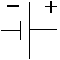
\includegraphics[scale=2]{immagini/fisica2/generatore}
\caption{simbolo della pila.}
\end{figure}

Calcoliamo il lavoro fatto dai due campi su una carica unitaria all'interno di un circuito chiuso:
\begin{equation}
  L = \oint (\ve E+\ve E_i)\cdot\ud\ve l = \oint \ve E_i\cdot\ud\ve l = \int_{\text{pila}}\!\!\!\! \ve E_i\cdot\ud\ve l + \int_{\text{circuito}} \underbrace{\ve E_i}_{=0}\cdot\ud\ve l = \int_{\text{pila}}\!\!\!\!\ve E_i\cdot\ud\ve l
 \end{equation}
avendo notato che la circuitazione del campo elettrostatico è nulla, mentre il campo impresso è nullo all'esterno della pila.
\begin{Def}[fem]
 La forza elettromotrice\index{forza!elettromotrice} è il lavoro fatto dal campo totale $\ve E+\ve E_i$ su una carica positiva unitaria che percorra una linea chiusa che passi per gli elettrodi della pila:
 \begin{equation}
  \text{fem} = \int_{\text{pila}} \ve E_i\cdot\ud\ve l
 \end{equation}

\end{Def}

\subsection{Resistenza interna}
Ogni generatore reale è caratterizzato da una resistenza interna $r$ e da una forza elettromotrice $\varepsilon$. Se gli colleghiamo un resistore con resistenza $R$ la circuitazione del campo elettrostatico deve essere nulla e quindi anche la variazione di potenziale. Allora se ai capi del generatore ideale c'è una differenza di potenziale $\varepsilon$ la caduta di tensione attraverso $R$ e $r$ deve essere uguale e contraria a $\varepsilon$. La differenza di tensione del generatore reale è minore di quella del generatore ideale e in particolare:
\[V_2-V_1=\varepsilon-Ir\]

Se in un ramo di circuito con estremi $A$ e $B$ ci sono dei resistori in serie e un generatore vale:
\begin{legge}[Ohm generalizzata\index{legge!di Ohm!generalizzata}]
\begin{equation}
V_A-V_B+\varepsilon=IR
\label{Ohm_gen}
\end{equation}
con $R=\sum R_i+r$.
\end{legge}
\subsubsection{Potenza massima}
Vogliamo sapere quando un circuito assorbe la potenza massima. Riassumiamo tutto il circuito con un resistore con resistenza $R$, che rappresenta il carico cioè tutte le resistenze collegate al generatore reale, un generatore ideale e una resistenza interna $r$. Sappiamo che la potenza è 
\[P=RI^2=R\left(\frac{\varepsilon}{R+r}\right)^2\]
Vogliamo sapere qual è l'$R$ ottimale per cui viene dissipata la potenza maggiore su $R$. Deriviamo in $R$:
\[\frac{\ud P}{\ud R}=\varepsilon^2\left[\frac{1}{(R+r)^2}-\frac{2R}{(r+R)^3}\right]\]
che ha uno zero per $r=R$.

Se $r$ è molto diverso da $R$ gran parte dell'energia viene dispersa su $r$, cioè all'interno del generatore.

\section{Effetto Joule\index{effetto!Joule}\index{Joule}}
L'effetto Joule può essere spiegato sia da un punto di vista macroscopico che microscopico utilizzando il modello del gas di elettroni liberi. L'effetto Joule avviene ogni qualvolta la corrente passa attraverso un resistore.
\subsection{Macroscopico}
Quando una carica $\ud q$ passa da un potenziale $V_B$ a un potenziale $V_A$ ci sarà una variazione di energia potenziale; per definizione:
\[\ud W=\ud q(V_B-V_A)\]
ma $\ud q=I(t)\ud t$, sostituendo:
\begin{legge}[Joule\index{legge!di Joule}]
\begin{equation}
\ud W=I(t)(V_B-V_A)\ud t
\end{equation}
\end{legge}
\subsubsection{corrente stazionaria}
Nel caso stazionario $I(t)=I$:
\[W=\int_0^t I(V_B-V_A)\ud t=I(V_B-V_A)t\]
se il conduttore è ohmnico $I=\frac{\Delta V}{R}$:
\[W=RI^2t\]
e la potenza:
\[P=\frac{\ud W}{\ud t}=I\Delta V=RI^2=\frac{\Delta V^2}{R}\]

\subsection{Microscopico}
Consideriamo un conduttore con $N$ portatori di carica nell'unità di volume.
\[
 L_e=\ve F\cdot\ve s
\]
la potenza:
\[
 P_e =\ve F\cdot\ve v
\]
considerando tutti gli elettroni nel volume $\ud v$, la potenza:
\[
  \ud P=\ve F\cdot\ve v=-eN\ud v\ve E\cdot \ve v = \ve E\cdot\ve J\ud v =\sigma E^2\ud v
\]
Si puo anche ragiornare come segue.  Il singolo elettrone ha in media $\tau^{-1}$ collisioni nell'unità di tempo. Quindi nell'elementino di volume $\ud v$ nel tempo $\ud t$ avvengono $N\frac{\ud v}{\tau}\ud t$ collisioni. Tra un urto e un altro un elettrone viene accelerato con una forza $-eE$ parallela al campo elettrico costante. Lo spostamento sarà $v_D\tau$ parallelo al campo elettrico. Allora il lavoro su un elettrone sarà
\[
 \ud L_e =\ve F\cdot\ve s=-e Ev_D\ud t
\]
e su tutti gli elettroni nel volume $\ud v$:
\[
 \ud L = -e Ev_D\ud t N\ud v
\]
Considerando tutti gli elettroni del volume $\ud v$ la potenza:
\[
 \ud P=-\frac{N\ud v}{\tau}eEv_d\tau
\]
Ricordando che:
\[v_D=-\frac{eE}{m\tau}\qquad\sigma=\frac{e^2N}{m}\tau\]
\[\ud P=\frac{e^2NE^2}{m}\tau\ud v=\sigma E^2\ud v\]
Se consideriamo un filo conduttore di lunghezza $l$ e sezione $S$ con una differenza di potenziale $V_A-V_B=El$.
\[P=\int_V\ud P=\sigma E^2\int_V\ud v=\sigma E^2(Sl)=\sigma\frac{\Delta V^2}{l^2}Sl=\sigma\frac{S}{l}\Delta V^2=\frac{\Delta V^2}{R}\]




\chapter{Campo induzione magnetica\index{campo!induzione magnetica}}
\minitoc
\section{Definizione}
Ogni punto dello spazio è caratterizzato oltre che da un campo $\ve E$ anche da un vettore di induzione magnetica $\ve B$. Su una carica $q$ con velocità $\ve v$ immersa in un campo magnetico $\ve B$ viene esercitata una forza:
\begin{equation}
\ve F=q\ve v\times\ve B
\label{magneto01}
\end{equation}
chiamata forza di Lorentz\index{Lorentz}\index{forza!di Lorentz}. Essa è diretta perpendicolarmente alla velocità e quindi allo spostamento, ne deriva che non compie lavoro; è massima quando la velocità è perpendicolare a $\ve B$ e nulla quando gli è parallela. Considerando anche un campo elettrostatico la forza totale risulta:
\begin{equation}
\ve F=q\left(\ve E+\ve v\times \ve B\right)
\end{equation}
\subsection{Definizione operativa}
Per misurare il campo elettrico è sufficiente effettuare una misura, per quello magnetico non è sufficiente. Ricaviamo dalla \eqref{magneto01} il campo magnetico, moltiplichiamo vettorialmente per $\ve v$:
\[\frac{\ve F\times\ve v}{q}=\left(\ve v\times\ve B\right)\times\ve v=\ve vB^2-\left(\ve v\cdot\ve B\right)\ve v\]
Allora\footnote{??!!}:
\[\ve B=\frac{\ve F\times\ve v}{qv^2}+c\ve v\]
Facciamo due misure usando $q$ e due velocità ortogonali $\ve v_1$, $\ve v_2$:
\[\ve B=\frac{\ve F_1\times \ve v_1}{qv_1^2}+c_1\ve v_1\qquad\ve B=\frac{\ve F_2\times\ve v_2}{qv_1^2}+c_2\ve v_2\]
Moltiplichiamole scalarmente per $v_1$:
\[\frac{\left(\ve F_1\times \ve v_1\right)\cdot\ve v_1}{qv_1^2}+c_1v_1^2=\frac{\left(\ve F_2\times\ve v_2\right)\cdot v_1}{qv_1^2}+c_2\underbrace{\left(\ve v_2\cdot \ve v_1\right)}_{0}\]
\[c_1=\frac{\left(\ve F_2\times\ve v_2\right)v_1}{qv_1^2v_2^2}\]
\[\ve B=\frac{\ve F_1\times\ve v_1}{qv_1^2}+\frac{\left(\ve F_2\times\ve v_2\right)\ve v_1}{qv_1^2v_2^2}\ve v_1\]
\subsection{Unità di misura}
\[[B]=[mlq^{-1}t^{-1}]=\frac{\newton\second}{\coulomb\meter}=\frac{\volt\second}{\meter\squared}=\frac{\weber}{\metre\squared}=T=\si{1E4}{\gauss}=10^4\,\text{gauss}\]\index{gauss}
Dove $\weber=\text{weber}={\volt\second}$, $\tesla=\text{tesla}=\frac{\weber}{\meter\squared}$.\index{weber}
\begin{Es}[elettrone in campo magnetico]
\label{es_Larmor}
Spariamo un elettrone in un campo magnetico $\ve B$ con velocità $\ve v_0=\ve v(0)$. Per semplicità scegliamo un sistema di riferimento in modo che $\ve B=B\ver k$ e che $\ve r(0)=0$. Ad ogni istante sull'elettrone agisce la forza di Lorentz:
\[\ve F(t)=-e\ve v(t)\times \ve B\]
Scomponiamo le componenti:
\[\left\{
\begin{array}{l}
ma_x=F_x=-e\left(v_yB_z-v_zB_y\right)=-ev_yB\\
ma_y=F_y=e\left(v_xB_z-v_zB_x\right)=ev_xB\\
ma_z=F_z=-e\left(v_xB_y-v_yB_x\right)=0\\
\end{array}\right.\]
riassumendo:
\[\left\{
\begin{array}{l}
\ddot x=-\frac{eB}{m}\dot y\\
\ddot y=\frac{eB}{m}\dot x\\
\ddot z=0\\
\end{array}\right.\]
che è un sistema di equazioni differenziali del second'ordine accoppiate. Operiamo la sostituzione $\frac{\ud}{\ud t}\ve r=\ve v$:
\[
\left\{
\begin{array}{l}
\dot v_x=-\omega v_y\\
\dot v_y=\omega v_x\\
\dot v_z=0\\
\end{array}\right.\]
con $\omega=\frac{eB}{m}$. L'ultima ha naturalmente soluzione:
\[z=v_{z_0}t\]
Deriviamo la prima:
\[\ddot v_x=-\omega\dot v_y=-\omega^2 v_x\]
e la seconda:
\[\ddot v_y=\omega\dot v_x=-\omega^2 v_y\]
Abbiamo disaccoppiato le equazioni. Una soluzione generale della prima è 
\[v_x=A\sin\left(\omega t+\varphi\right)\]
Sostituendo troviamo anche la seconda:
\[v_y=-A\cos\left(\omega t+\varphi\right)\]
La forza di Lorentz non compie lavoro, quindi si deve conservare l'energia cinetica essendo $v_z$ costante si deve conservare la quantità 
\[v_x^2+v_y^2=v_{x_0}^2+v_{y_0}^2=v_\perp^2\]
Allora $A=v_\perp$. Manca da ricavare $\varphi$:
\[\left\{\begin{array}{l}
v_x=v_\perp\sin\left(\omega t+\varphi\right)\\
v_y=-v_\perp\cos\left(\omega t+\varphi\right)
\end{array}\right.\]
Imponendo che $\ve v(0)=\ve v_0$:
\[\left\{\begin{array}{l}
v_x(0)=v_\perp\sin\left(\varphi\right)=v_{x_0}\\
v_y(0)=-v_\perp\cos\left(\varphi\right)=v_{y_0}
\end{array}\right.\]
Dividendo:
\[\varphi=\arctan{\left(-\frac{v_{x_0}}{v_{y_0}}\right)}\]
Per trovare $x$, $y$ basta integrare, si trova:
\[\left\{
\begin{array}{l}
x=-\frac{v_\perp}{\omega}\cos\left(\omega t+\varphi\right)\\
y=-\frac{v_\perp}{\omega}\sin\left(\omega t+\varphi\right)\\
z=v_{z_0}t\\
\end{array}\right.\qquad\text{con}\qquad
\begin{array}{l}
v_\perp=\sqrt{v_{x_0}^2+v_{y_0}^2}\\
\omega=\frac{eB}{m}\\
\varphi=\arctan{\left(-\frac{v_{x_0}}{v_{y_0}}\right)}\\
\end{array}\]
\`E l'equazione di un elica con asse parallelo a $\ve B$. Se si considera solo la proiezione sul piano $xy$ si trova una circonferenza con raggio:
\[r_L=\frac{v_\perp}{\omega}\]
chiamato raggio di Larmor\index{raggio!di Larmor}\index{Larmor}.
\end{Es}
\begin{Es}[spettrometro di massa\index{spettrometro!di massa}]\label{spettrometro01}
Lo spettrometro di massa è uno strumento che consente di determinare con alta precisione la massa di particelle cariche, per esempio ioni.
\begin{figure}[htbp]
\centering
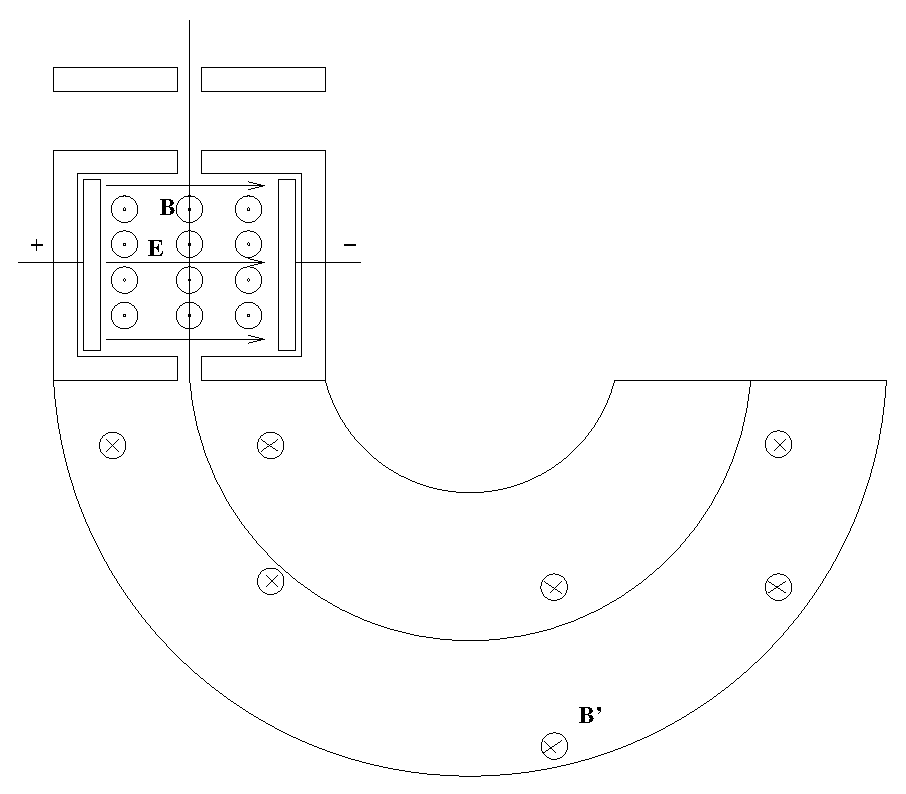
\includegraphics[scale=0.5]{immagini/fisica2/spettrometro}
\caption{spettrometro di massa.}
\end{figure}
La prima parte è detta separatore di velocità \index{separatore!di velocità}. Le particelle focalizzate da fenditure entrano con velocità casuale e vengono sottoposte a un campo magnetico $\ve B$ e uno elettrico $\ve E$ ortogonali. La forza risultante è 
\[F=q(E+vB)\]
essendo $\ve v\perp\ve B$. Solo le particelle che hanno una certa velocità e cioè 
\[v=\frac{E}{B}\]
non sono deviate dai campi e quindi riescono a uscire dal separatore di velocità  Nella seconda parte le particelle cariche subiscono una deviazione dovuta al campo magnetico $\ve B\,'$. Misurando dove le particelle colpiranno lo schermo si può dedurre il raggio di Larmor e ricavare la massa:
\[m=\frac{qB'B}{E}r_L\]
\end{Es}

\begin{Es}[Ciclotrone]
 Il ciclotrone \index{ciclotrone} è un acceleratore inventato negli anni 30. È formato da due conduttori cavi semicilindrici a forma di D, che uniti formano un ciclindro. Tra le due cavità è applicata una differenza di potenziale varibile in modo alternato $V=V_0\sin\omega_{RF}t$ dove $RF$ sta per radiofrequenza. Inoltre è applicato un campo magnetico ortogonale alle cavità.
 
 Il processo inizia iniettando uno ione di massa $m$ e carica $q$ da una sorgente al centro del sistema. Esso viene accelerato dalla differenza di potenziale tra le due D a una velocità finale $v_1$ che si può ricavare dalla conservazione dell'energia:
 \[
  \frac{1}{2}mv_1^2 = qV
 \]
 quindi $v_1^2 = \frac{2qV}{m}$. Lo ione entra in $D_1$ dove il campo elettrico è nullo, e viene deviato dalla forza di Lorentz su una traiettoria circolare di raggio $r_1=\frac{m v_1}{qB}$. Il tempo che ci impiegherà ad uscire da $D_1$ sarà:
 \[
  t_1 = \frac{\pi r_1}{v_1}=\frac{\pi m}{qB}
 \]
 come si nota questo tempo non dipende dalla velocità della particella. Nello stesso tempo la tensione (la radiofrequenza) ha cambiato segno e quindi lo ione viene accelerato passando da $D_1$ a $D_2$. Ad ogni semigiro lo ione acquista un'energia cinetica $qV$. Dentro a $D_2$ lo ione compie una semicirconferenza con raggio maggiore rispetto a prima: $r_2={m v_2}{qB}$ e ci impiega:
 \[
  t_2 = \frac{\pi r_2}{v_2}=\frac{\pi m}{qB} = t_1 = \Delta t
 \]
 infatti come già sottolineato il tempo di percorrenza di un'orbita circolare in un campo magnetico non dipende dalla velocità della particella. Il grande vantaggio del ciclotrone è che la particella ci mette sempre lo stesso tempo a percorrere metà circonferenza. La velocità angolare della particella è:
 \[
  \omega = \frac{2\pi}{T} = \frac{2\pi}{2\Delta t} = \frac{\pi}{\Delta t} = \frac{qB}{m}
 \]

 quindi si può ottenere un'accelerazione se il tempo impiegato dalla particella a fare una semicirconferenza è pari al semiperiodo di $V$:
 \[
  \Delta t = \frac{T_{RF}}{2} = \frac{\pi}{\omega_{RF}}
 \]
 questo vuol dire $\omega_{RF}=\omega$, cioè la pulsazione della radiofrequenza, detta pulsazione di ciclotrone, deve essere pari alla velocità angolare dello ione.
 
 Il processo continua fino a quando lo ione non arriva alla circonferenza massima di raggio $R$, quindi:
 \[
  v_{\max} = \frac{qBR}{m}
 \]
 cioè un'energia cinetica massima di:
 \[
  E_{\max} = \frac{1}{2}mv_{\max}^2 = \frac{q^2 B^2 R^2}{2m}
 \]
 Ad ogni giro lo ione guadagna un'energia pari a $2qV$, quindi il numero di giri necessari è:
 \[
  N = \frac{E_{\max}}{2qV} = \frac{qB^2R^2}{4mV}
 \]
 e quindi un tempo:
 \[
  t_{\max} = 2\Delta tN = \frac{\pi R^2 B}{2V}
 \]
 
 Il limite a questo acceleratore è dato dalla relatività, infatti $\omega$ non è costante, ma pari a $\frac{qB}{\gamma m}$. Poiché $\gamma$ cresce con la velocità allora $\omega$ decresce e non è più in fase con $\omega_{RF}$. Si riesce quindi ad accelerare una particella solo fino a qualche decina di $\MeV$. Il sincrociclotrone risolve questo problema modificando $\omega_{RF}$ in base alla velocità della particella e si possono raggiungere centinaia di $\MeV$.
\end{Es}


\section{Forza magnetica su una corrente\index{forza!magnetica!su corrente}}
Sperimentalmente si trova che su un filo di lunghezza $l$, sezione $S$ percorso dalla corrente stazionaria $I$, immerso in un campo magnetico uniforme $\ve B$ agisce una forza:
\begin{equation}
\ve F=I\ve l\times \ve B
\label{forza_filo}
\end{equation}
$\ve l$ è il vettore con modulo $l$ e verso e direzione quello della corrente positiva. La cosa può essere dimostrata partendo dalla \eqref{magneto01}. Su ogni elettrone agisce una forza di Lorentz:
\begin{equation}
\ve F_e=-e\ve v_D\times\ve B
\label{forza_lorentz_e}
\end{equation}
Quindi la forza sul filo è la somma delle forze \eqref{forza_lorentz_e} su tutti gli elettroni. Se $N$ è il numero di elettroni nell'unità di volume e il volume $V=Sl$:
\begin{equation}
\ve F=-NSle\ve v_D\times\ve B
\label{forza_lorentz_e2}
\end{equation}
L'espressione \eqref{forza_lorentz_e2} può essere semplificata ricordando che per definizione la densità di corrente è 
\[
\ve J=-Ne\ve v_D
\]
\begin{equation}
\ve F=-NSle\ve v_D\times\ve B=Sl\ve J\times\ve B
\end{equation}
L'intensità di corrente è 
\[I=\iint_S \ve J\cdot \ve n\,\ud a=JS=Nev_DS\]
Dunque la forza per unità di volume è $\ve J\times\ve B$. Ora possiamo definire $\ve l$ con modulo $l$ e direzione e verso quelli di $\ve J$, dunque:
\begin{equation}
\ve F=SJ\ve l\times\ve B=I\ve l\times \ve B
\label{forza_lorentz_3}
\end{equation}
che è proprio la \eqref{forza_filo} e può essere usata come definizione di $\ve B$. Potremmo anche definire un vettore $\ve I=S\ve J$ e la forza per unità di lunghezza sarebbe $\ve I\times\ve B$.
\subsection{Seconda formula di Laplace}
Per passare dalla \eqref{forza_lorentz_e} alla \eqref{forza_lorentz_e2} bisogna supporre che $\ve B$ sia uniforme e quindi $F_e$ è uguale per ogni elettrone. Nel caso più generale, la forza che si esercita su un elemento infinitesimo $\ud l$ è 
\begin{equation}
\ud \ve F=I\ud \ve l\times \ve B
\end{equation}
La seconda formula di Laplace\index{Laplace}\index{seconda formula di Laplace} non è semplicemente il differenziale della forza~\eqref{forza_lorentz_3}. Allora:
\begin{equation}
\ve F=\oint_C I\ud\ve l\times B
\label{forza_lorentz_4}
\end{equation}
è la forza su tutto il circuito $C$. Dato che $I\ud \ve l=\ve JS\ud l=\ve J\ud v$ la \eqref{forza_lorentz_4} diventa:
\begin{equation}
\ve F=\int_V\ve J\times\ve B\,\ud v
\end{equation}
\begin{Es}[effetto Hall]
L'effetto Hall avviene nei conduttori percorsi da corrente in un campo magnetico $\ve B$. Immaginiamo una lastra conduttrice di larghezza $w$ e altezza $t$. Sia $v_D$ la velocità di deriva degli elettroni. Essi saranno deviati con una forza:
\[\ve F=-e\ve v_D\times \ve B\]
\begin{figure}[htbp]
\centering
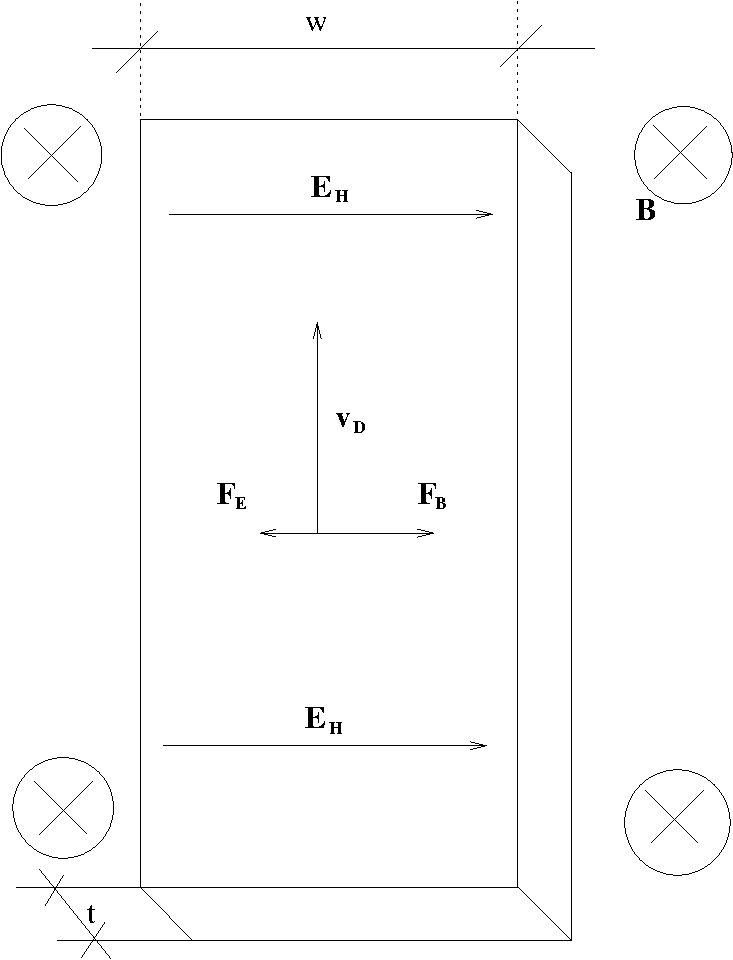
\includegraphics[scale=0.4]{immagini/fisica2/Hall}
\end{figure}
Si crea allora un accumulo di cariche da un lato e del segno opposto sull'altro: si crea un campo elettrico $\ve E_H$ ortogonale alla direzione della corrente. Tra i due lati della lastra di è formata una differenza di potenziale $\Delta V_H=E_Hw$. Il sistema raggiunge l'equilibrio quando la forza sugli elettroni:
\[\ve F=-e\ve v_D\times B-e\ve E_H\]
è nulla cioè quando la forza del campo elettrico è uguale e contraria alla forza di Lorentz. Ricordando che la velocità è ortogonale al campo magnetico e al campo elettrico:
\[E_H=v_DB\]
Ricordando l'espressione di $v_D$:
\[v_D=\frac{J}{Ne}=\frac{I}{SNe}=\frac{I}{wtNe}\]
\[\Delta V_H=E_Hw=\frac{I}{tNe}B\]
Si può definire una\index{resistenza!di Hall} resistenza di Hall:
\[
 R_H = \frac{\Delta V_H}{I}=\frac{1}{tNe}B
\]
\end{Es}

\section{Momento su un circuito\index{momento!su un circuito}}
Sia $C$ un circuito piano chiuso attraversato da una corrente stazionaria $I$ immerso in un campo magnetico $\ve B$ uniforme. Dalla \eqref{forza_lorentz_4} deduciamo che sulla spira agisce una forza nulla:
\[\ve F=\oint_C I\ud\ve l\times\ve B=I\oint_C\ud \ve l\times\ve B=I\left(\oint_C\ud\ve l\right)\times\ve B=0\]
in quanto $0=\oint_C \ud \ve l\neq\oint_C\ud l$. Scegliamo un sistema di riferimento $xyz$ in modo che il piano $xy$ contenga $C$ e la proiezione di $\ve B$ sia parallela all'asse $x$; sia $\theta$ l'angolo che $\ve B$ forma con $z$. Allora:
\[B_z=B\cos\theta\qquad B_x=B\sin\theta\]
Suddividiamo il circuito in tante strisce infinitesime. Se la corrente di $C$ gira in verso antiorario, anche quella nelle strisce; in questo modo i lati adiacenti si cancellano. Ogni spira a causa del campo magnetico è soggetta ad una forza:
\[\ud\ve F=I\ud\ve l\times\ve B\]
\[\norm{\ud\ve F}=I\ud lB_x\sin\alpha=\ud yB\sin\theta I\]
Dunque la forza è massima quando la spira è perpendicolare al campo magnetico.
\[\ud \ve M=IlB\ud y\sin\theta\ve n=I\ud a B\ve n\]
\[\ud m=I\ud a\ve n\]
\[\ud\ve M=\ud\ve m\times\ve B\]
\[\ve M=\iint_S\ud\ve m\times \ve B=\iint I\ud a\ve n\times B=I\ve n\left(\iint_S\ud a\right)\times \ve B=IS\ve n\times \ve B\]
Definiamo il momento di dipolo magnetico\index{momento!di dipolo magnetico}:
\[\ve m=IS\ve n\]
allora:
\[\ve M=\ve m\times \ve B\]
che ricorda l'analoga espressione per il dipolo elettrico: $\ve M=\ve p\times\ve E$.
\section{Ago magnetico\index{ago magnetico}}
Un ago magnetico immerso in un campo magnetico costante $\ve B$ si comporta come un circuito, cioè subisce un momento che lo fa disporre parallelamente alle linee del campo:
\[\ve M=\ve K\times\ve B\]
con $\ve K$ è un vettore che dipende dalle caratteristiche dell'ago, ed è orientato secondo la linea polo sud, polo nord dell'ago.

Il suo comportamento è analogo a quello del dipolo elettrico, con momento di dipolo $\ve p=q\delta$. Possiamo immaginare l'ago magnetico come costituito da due cariche magnetiche di segno opposto $q_m$, una al polo nord e l'altra al polo sud. Definiamo $\ve m$ momento magnetico dell'ago in modo tale che:
\[\ve K=\ve m=q_m \ve\delta\]
\begin{figure}[htbp]
\centering
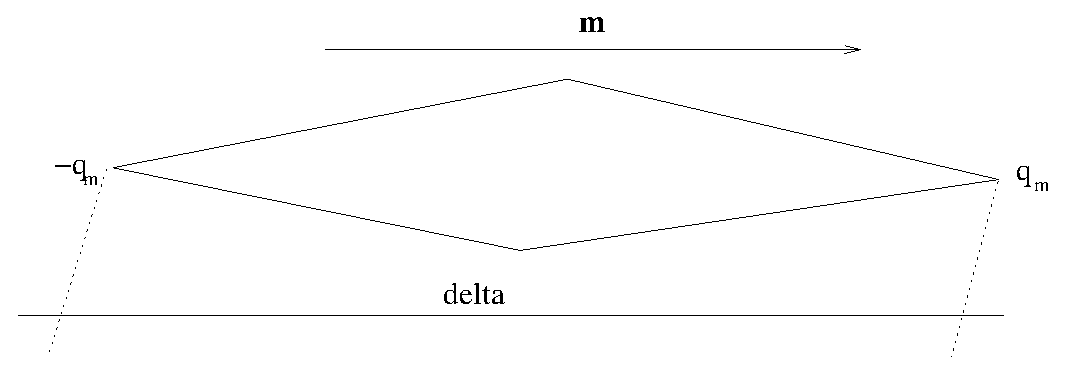
\includegraphics[scale=0.5]{immagini/fisica2/ago}
\end{figure}
\subsection{Lamina magnetica\index{lamina!magnetica}}
Suddividiamo una spira di area $S$ in infinitesime spire di area $\ud a$. Ogni spira avrà un momento magnetico $\ud\ve m=I\ud a\ve n$. Per analogia con il dipolo possiamo anche dire che $\ud\ve m=\sigma_m\ud a \ve \delta$ e allora:
\[\sigma_m=\frac{I}{\delta}\]
rappresenta la densità di carica magnetica sulle facce di una lamina magnetica con lamine a distanza $\delta$, che a grande distanza è equivalente alla spira iniziale.

\section{Campi magnetici generati da correnti\index{campi magnetici!generati da correnti}}
Una corrente crea un campo magnetico. Al posto di usare una carica di prova per esplorare il campo, si può usare un aghetto magnetico di prova. Si scopre che un filo rettilineo crea un campo magnetico le cui linee di forza si chiudono su se stesso.
\subsection{Legge di Biot--Savart\index{Biot}\index{Savart}\index{legge!di Biot--Savart}}
\begin{legge}[Biot--Savart]
Per un filo infinito percoso da corrente $I$ vale
\begin{equation}
 B=k\frac{I}{r}
\end{equation}
\end{legge}
con $k$ una costante che dipende dalle unità di misura. Il primo modo è porre $k=1$, in realtà si pone:
\[k=\frac{\mu_0}{2\pi}\]
con $\mu_0$ la permeabilità magnetica del vuoto:
\[
\mu_0=\si[numaddn=\pi]{4\pi e-7}{\henry\per\meter}
\]
Quanto detto vale per il modulo, essendo il campo magnetico attorno al filo, allora:
\[\ve B\left(\ve r\right)=\frac{\mu_0}{2\pi}\frac{\ver s\times\ve r}{r^2}I\]
con $\ver s$ è un versore orientato come il verso della corrente, mentre $\ve r$ è il vettore che individua il punto rispetto al filo, ha quindi il modulo della distanza tra il filo e il punto.
\subsubsection{unità di misura\index{weber}}
\[\left[\mu_0\right]=\frac{\text{weber}}{\text{metro}\cdot\text{ampere}}=\frac{\volt\second}{\meter\ampere}=\frac{\ohm\second}{\meter}=\frac{\henry}{\meter}\]
con:
\[\henry=\text{ohm}\cdot\text{secondo}=\text{henry}\]
\subsection{Prima formula di Laplace\index{prima formula di Laplace}\index{Laplace}}
La prima legge di Laplace stabilisce che un elemento $\ud \ve l$ di circuito percorso da una corrente $I$ produce in un punto $P$ distate $\ve r$ da esso un vettore di induzione magnetica:
\begin{equation}
\ud\ve B\left(\ve r\right)=\frac{\mu_0}{4\pi}I\frac{\ud\ve l\times\left(\ve r-\ve r\,'\right)}{\norm{\ve r-\ve r\,'}^3}
\end{equation}
Per un circuito generico possiamo usare il principio di sovrapposizione con tutti gli elementini $\ud\ve l$  del circuito:
\begin{equation}
\ve B\left(\ve r\right)=\frac{\mu_0}{4\pi}\oint_C I\frac{\ud\ve l\times\left(\ve r-\ve r\,'\right)}{\norm{\ve r-\ve r\,'}^3}
\label{campo_spira_laplace}
\end{equation}
Se il conduttore non è filiforme, essendo $I\ud \ve l=\ve J\ud v$:
\begin{equation}
\ve B\left(\ve r\right)=\frac{\mu_0}{4\pi}\int\frac{\ve J\left(\ve r\,'\right)\times\left(\ve r-\ve r\,'\right)}{\norm{\ve r-\ve r\,'}^3}\,\ud v'
\end{equation}
\begin{Es}[filo infinito\index{filo infinito}]
\label{Es:filo_infinito}
Ricaviamo la legge di Biot--Savart. Chiamiamo $\ve r$ la distanza di $P$ dall'elementino $\ud l$ e $R$ la distanza dal filo. Allora:
\begin{figure}[htbp]
\centering
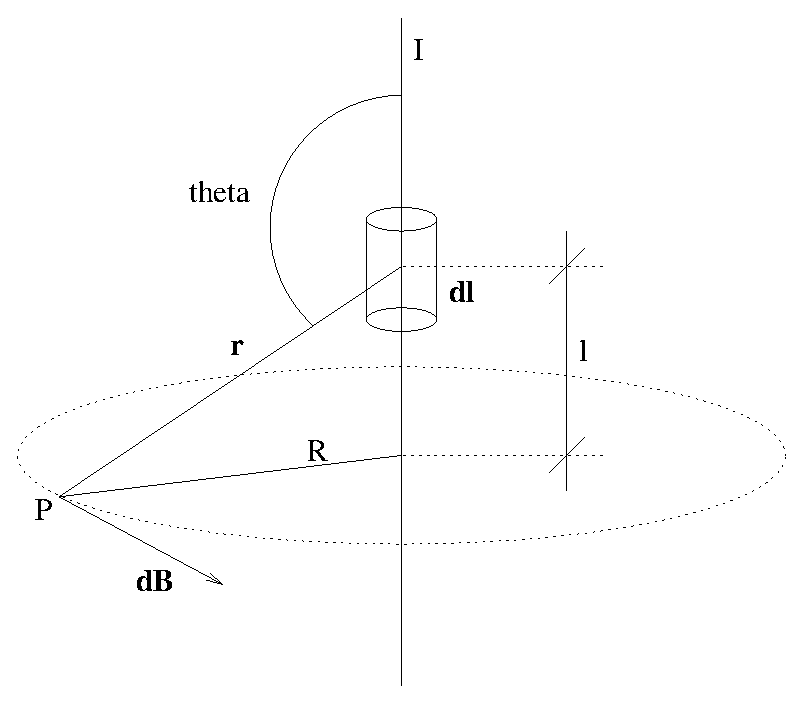
\includegraphics[scale=0.5]{immagini/fisica2/magneto_filo}
\end{figure}
\[\ud \ve B\left(\ve r\right)=\frac{\mu_0}{4\pi}I\frac{\ud\ve l\times\ve r}{\norm{\ve r}^3}\qquad\ud B\left(\ve r\right)=\frac{\mu_0}{4\pi}I\frac{\ud l\sin\theta}{r^2}\]
ma:
\[r=\frac{R}{\sin\theta}\qquad l=\frac{R}{\tan\left(\pi-\theta\right)}=-\frac{R}{\tan\theta}\qquad \ud l=\frac{R}{\sin^2\theta}\ud\theta\]
\end{Es}
\begin{align*}
B\left(\ve r\right)&=\frac{\mu_0}{4\pi}I\int_{-\infty}^{+\infty}\frac{\sin\theta}{r^2}\,\ud l=\frac{\mu_0}{4\pi}I\int_{0}^{\pi}\frac{\sin\theta\sin^2\theta}{R^2}\frac{R}{\sin^2\theta}\ud\theta\\
&=\frac{\mu_0}{4\pi}\frac{I}{R}\int_0^\pi\sin\theta\,\ud\theta=\frac{\mu_0}{2\pi}\frac{I}{R}
\end{align*}
in forma vettoriale:
\begin{equation}
\ve B(\ve r)=\frac{\mu_0}{2\pi}\frac{I}{\norm{\ve r}}\ver{s}\times{\ver e_r}
\end{equation}
\begin{Es}[spira circolare\index{spira}]
Consideriamo un circuito di forma circolare, con raggio $R$. Vogliamo il campo magnetico lungo l'asse. Per ragioni di simmetria il campo magnetico risultate è ortogonalmente al piano della spira. Usiamo le coordinate cilindriche. $P$ avrà coordinate $(0,0,w)$, individuato dal vettore $\ve r=w \ver e_w$, mentre l'elementino $\ud l$ della spira sarà individuato dal vettore $\ve r\,'=r'\ver e_r$. L'elementino $\ud\ve l=R\ud\theta\ver e_\theta$.
\[\ve B\left(\ve r\right)=\frac{\mu_0}{4\pi}\int_l\frac{I\ud\ve l\times\left(\ve r-\ve r\,'\right)}{\norm{\ve r-\ve r\,'}^3}=\frac{\mu_0}{4\pi}\int_0^{2\pi}\frac{IR\ud\theta\ver e_\theta\times\left(w\ver w_z-R\ver e_r\right)}{\left(R^2+w^2\right)^{\frac{3}{2}}}\]
Ricordando che:
\[\ver e_\theta\times\ver e_w=\ver e_r\qquad \ver e_\theta\times\ver e_r=-\ver e_w\qquad \int_0^{2\pi} \ud\theta\ver e_r=\int_0^{2\pi}\left(\cos\theta\ver \imath+\sin\theta\ver \jmath\right)\,\ud \theta=0\]
\begin{equation}
 \label{eq:b_spira}
 \begin{aligned}
  \ve B\left(w\right)&=\frac{\mu_0IR}{4\pi\left(R^2+w^2\right)^{\frac{3}{2}}}\int_0^{2\pi}\left(w\ver e_r+R\ver e_w\right)\ud\theta=\frac{\mu_0IR}{4\pi\left(R^2+w^2\right)^{\frac{3}{2}}}R\ver e_w 2\pi\\
&=\frac{\mu_0}{2}\frac{IR^2}{\left(R^2+w^2\right)^{\frac{3}{2}}}\,\ver e_w
 \end{aligned}
\end{equation}
Nel caso particolare $w=0$ si ha:
\[\ve B=\frac{\mu_0}{2}\frac{I}{R}\,\ver e_w\]
\end{Es}
\begin{Es}[solenoide\index{solenoide}]
Immaginiamo il solenoide come l'insieme di tante spire affiancate e usiamo il principio di sovrapposizione. Sia $N$ il numero di spire per unità di lunghezza, $l$ la sua lunghezza. Il campo magnetico generato da una spira che non si trovi nell'origine, ma ad una distanza $w'$ sull'asse è (dalla \eqref{eq:b_spira}):
\[
 \ve B_S(w,w')=\frac{\mu_0}{2}\frac{IR^2}{\left(R^2+\left(w-w'\right)^2\right)^{\frac{3}{2}}}\,\ver e_w
\]
Essendo $N\ud w'$ il numero di spire in $\ud w'$:
\begin{equation*}
\ve B(w)=\int_{-\frac{l}{2}}^{\frac{l}{2}}\ve B_S(w,w')N\,\ud w'=\frac{\mu_0INR^2}{2}\ver e_w\int_{-\frac{l}{2}}^{\frac{l}{2}}\frac{\ud w'}{\left(R^2+\left(w-w'\right)^2\right)^{\frac{3}{2}}}
\end{equation*}
Occupiamoci dell'integrale, usiamo la sostituzione $u=w-w'$ quindi $\ud u=-\ud w'$:
\[
 \int\frac{\ud w'}{\left(R^2+\left(w-w'\right)^2\right)^{\frac{3}{2}}} = -\int\frac{\ud u}{\left(R^2+u^2\right)^{\frac{3}{2}}} = -\frac{1}{R^3}\int\frac{\ud u}{\left(1+\left(\frac{u}{R}\right)^2\right)^{\frac{3}{2}}}
\]
Sostituendo ora $\frac{u}{R}=\sinh t$, $\ud u=R\cosh t\ud t$:
\[\int\ldots = -\frac{1}{R^3}\int\frac{R\cosh t}{\left(1+\sinh^2t\right)^{\frac{3}{2}}}\ud t=-\frac{1}{R^2}\int\frac{\ud t}{\cosh^2 t}=-\frac{1}{R^2}\tanh t\]
Risostituiamo all'indietro:
\begin{align*}
-\frac{1}{R^2}\tanh t&=-\frac{1}{R^2}\frac{\sinh\arcsinh\frac{u}{R}}{\cosh\arcsinh\frac{u}{R}}=-\frac{u}{R^3}\frac{1}{\sqrt{1+\sinh^2\arcsinh\frac{u}{R}}}\\
&=-\frac{u}{R^3}\frac{1}{\sqrt{1+\left(\frac{u}{R}\right)^2}}=-\frac{1}{R^3}\frac{w-w'}{\sqrt{1+\left(\frac{w-w'}{R}\right)^2}}
\end{align*}
Allora:
\begin{align*}
\ve B(w)&=\frac{\mu_0NIR^2}{2}\ver e_w\left[\frac{1}{R^3}\frac{w'-w}{\sqrt{1+\left(\frac{w'-w}{R}\right)^2}}\right]_{w'=-\frac{l}{2}}^\frac{l}{2}\\
&=\dfrac{\mu_0NI}{2R}\ver e_w\left(\dfrac{w+\frac{l}{2}}{\sqrt{1+\left(\frac{w+\frac{l}{2}}{R}\right)^2}}-\dfrac{w-\frac{l}{2}}{\sqrt{1+\left(\frac{w-\frac{l}{2}}{R}\right)^2}}\right)
\end{align*}
che rappresenta il campo magnetico generato da un solenoide di lunghezza $l$, se $l\to\infty$:
\begin{equation}
 \ve B=\mu_0IN\ver e_w 
\end{equation}
Infatti per esempio, usando al primo passaggio H\^{o}pital:
\begin{multline*}
 \lim_{l\to\infty}\dfrac{w\pm\frac{l}{2}}{\sqrt{1+\left(\frac{w\pm\frac{l}{2}}{R}\right)^2}}=
 \lim_{l\to\infty}\frac{\pm\frac{1}{2}}{\frac{1}{2}\left(1+\left(\frac{w\pm l/2}{R}\right)^2\right)^{-1/2} 2\left(\frac{w\pm l/2}{R}\right)\frac{\pm 1}{2 R}}\\
 =\lim_{l\to\infty}\frac{\frac{w \pm l/2}{R}\sqrt{\left(\frac{R}{w\pm l/2}\right)^2+1}}{2\frac{w\pm l/2}{R}\frac{\pm 1}{2R}}=\lim_{l\to\infty}\frac{\sqrt{\left(\frac{R}{w\pm l/2}\right)^2+1}}{2\frac{\pm 1}{2R}}=\pm R
\end{multline*}
\end{Es}
\begin{Es}[Spira rettangolare]
 Sia una spira rettangolare di lati $a$, $b$ percorsa dalla corrente $I$. Vogliamo calcolare il campo magnetico generato lungo il suo asse, al variare di $z$.
\begin{figure}[htbp]
 \centering
 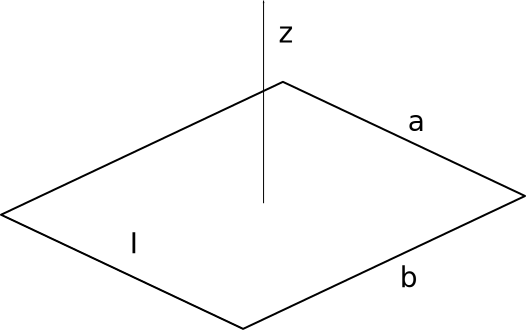
\includegraphics[scale=0.4]{immagini/fisica2/spira_rettangolare}
 % spira_quadrata.pdf: 421x264 pixel, 72dpi, 14.85x9.31 cm, bb=0 0 421 264
\end{figure}
È opportuno calcolare prima il campo generato da ciascun lato. Prendiamo quindi un filo di lunghzza $l$ e calcoliamo il campo sul suo asse, ad una distanza $R$, che cosideriamo l'origine del nostro sistema ($\ve r=0$).
\begin{figure}[htbp]
 \centering
 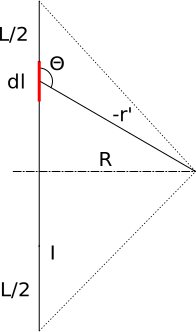
\includegraphics[scale=0.6]{immagini/fisica2/filo_spiraquadrata}
 % filo_spiraquadrata.pdf: 157x266 pixel, 72dpi, 5.54x9.38 cm, bb=0 0 157 266
\end{figure}
Il campo generato da un elementino:
\[
 \ud\ve B = \frac{\mu_0}{4\pi}I\frac{\ud\ve l\times(\ve r-\ve r')}{\norm{\ve r-\ve r'}^3}=\frac{\mu_0}{4\pi}I\frac{\ud\ve l\times(-\ve r')}{r'^3}
\]
il modulo:
\[
 \ud B = \frac{\mu_0}{4\pi}I\frac{\ud l\sin\theta}{r'^2}
\]
scriviamo tutto in funzione dell'angolo $\theta$, variabile sulla quale integreremo:
\[
 \frac{1}{r'^2} = \frac{\sin^2\theta}{R^2}\qquad l = -R\cot\theta\qquad\ud l = \frac{R}{\sin^2\theta}\ud\theta
\]
\[
 \ud B = \frac{\mu_0}{4\pi}I\frac{\sin\theta}{R}\,\ud\theta
\]
Il campo totale\footnote{Si poteva anche integrale in $\ud l$ tra $\pm\frac{L}{2}$ usando $r'=\sqrt{R^2+l^2}$ e $\sin\theta=\frac{R}{\sqrt{R^2+l^2}}$:
\[
 B = \frac{\mu_0}{4\pi}I\int_{-\frac{L}{2}}^{\frac{L}{2}}\ud l\frac{R}{(R^2+l^2)^{3/2}}=\frac{\mu_0}{4\pi}\frac{I}{R}\int\frac{1}{\cosh^2 x}\,\ud x=\frac{\mu_0}{4\pi}\frac{I}{R}\left[\frac{l/R}{\sqrt{1+\left(l/R\right)^2}}\right]_{-L/2}^{L/2}
\]
avendo usato la sostituzione $\sinh x=\frac{l}{R}$.
}:
\[
 B = \frac{\mu_0}{4\pi R}I\int_{\theta_\text{min}}^{\theta_\text{max}}\sin\theta\ud\theta
\]
con $\theta_\text{min}\in (0,\frac{\pi}{2})$ e $\theta_\text{max}\in (\frac{\pi}{2},\pi)$. Per simmetria il campo generato dalla metà inferiore del filo è uguale a quello generato dalla parte superiore:
\[
 B = 2\left[\frac{\mu_0}{4\pi R}I\int_{0}^{\theta_\text{max}}\sin\theta\ud\theta\right]= 2\left[-\frac{\mu_0}{4\pi R}I\cos\theta_\text{max}\right]=\frac{\mu_0}{2\pi R}I\frac{L/2}{\sqrt{R^2+(L/2)^2}}
\]
con
\[
 \cos(\pi-\theta_\text{max})=-\cos\theta_\text{max} = \frac{L/2}{r_\text{max}'}=\frac{L/2}{\sqrt{R^2+(L/2)^2}}
\]
vettorialmente:
\[
 \ve B = \frac{\mu_0}{2\pi R}I\frac{L/2}{\sqrt{R^2+(L/2)^2}}\ver u_\theta
\]
Fin qui, abbiamo in pratica rifatto l'esempio \ref{Es:filo_infinito}. Ritornando alla spira rettangolare l'unica cosa da fare è sommare i contributi dei singoli lati:
\begin{align*}
 B_1 = B_3 &= \frac{\mu_0}{2\pi R_b}I\frac{b/2}{\sqrt{R_b^2+(b/2)^2}}\\
 B_2 = B_4 &= \frac{\mu_0}{2\pi R_a}I\frac{a/2}{\sqrt{R_a^2+(a/2)^2}}\\
\end{align*}
\begin{figure}[htbp]
 \centering
 \subfigure{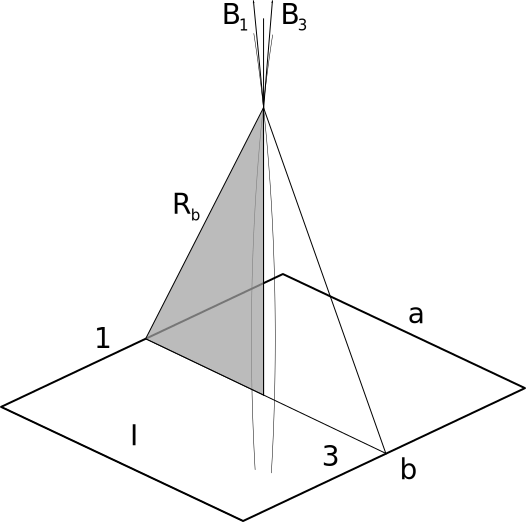
\includegraphics[scale=0.4]{immagini/fisica2/spira_rettangolare2}}
 % spira_rettangolare2.pdf: 421x418 pixel, 72dpi, 14.85x14.75 cm, bb=0 0 421 418
 \qquad
 \subfigure{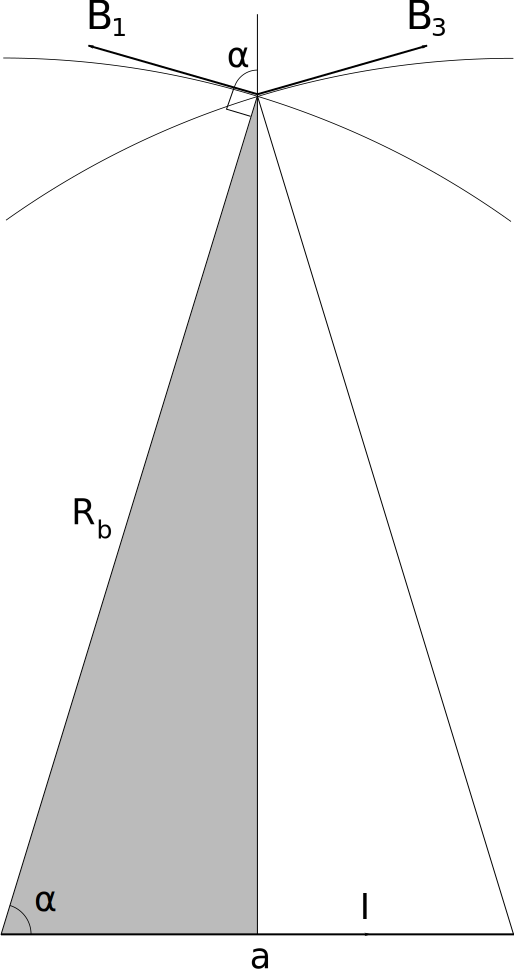
\includegraphics[scale=0.2]{immagini/fisica2/spira_rettangolare3}}
\end{figure}
con:
\[
 R_b = \sqrt{z^2+(a/2)^2}\qquad R_a = \sqrt{z^2+(b/2)^2}
\]
Sommando vettorialmente le uniche componenti che non si annullano sono quelle lungo l'asse $z$:
\[
 B_{1,z} = B_{3,z} = B_1\cos\alpha\qquad\cos\alpha = \frac{a/2}{R_b}
\]
l'angolo $\alpha$ tra $\ve B_1$ e l'asse $z$ è lo stesso tra la base $a$ e l'ipotenusa $R_b$ del triangolo evidenziato in figura; questo perché sono legati da una rotazione di 90 gradi (la tangente e il raggio sono sempre perpendicolari).
\[
 B_{1,z} = B_{3,z} = \frac{\mu_0}{8\pi}\frac{I}{R_b^2}\frac{ab}{\sqrt{R_b^2+(b/2)^2}} = \frac{\mu_0}{8\pi}\frac{I}{z^2+(a/2)^2}\frac{ab}{\sqrt{z^2+(a/2)^2+(b/2)^2}}
\]
e analogamente per gli altri due lati. Infine il campo totale:
\[
 \ve B = 2\frac{\mu_0}{8\pi}\frac{Iab}{\sqrt{z^2+(a/2)^2+(b/2)^2}}\left[\frac{1}{z^2+(a/2)^2}+\frac{1}{z^2+(b/2)^2}\right]\ver u_z
\]
a grande distanza, $z\gg a,b$:
\[
 \ve B (z\gg a,b) = \frac{\mu_0}{2\pi}\frac{Iab}{|z|^3}\ver u_z
\]
se introduciamo il momento magnetico della spira $\ve m=Iab\ver u_z$:
\[
 \ve B (z\gg a,b) = \frac{\mu_0}{4\pi}\frac{2\ve m}{|z|^3}
\]
\begin{figure}[htbp]
 \centering
 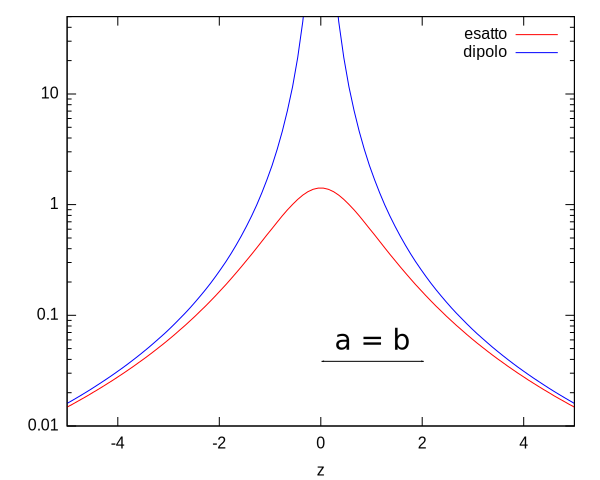
\includegraphics[scale=0.5]{immagini/fisica2/potenziale_spira_rettangolare}
 % potenziale_spira_rettangolare.: 480x384 pixel, 72dpi, 16.93x13.55 cm, bb=0 0 480 384
 \caption{Potenziale di una spira quadrata di lato $a=2$ esatto e in approssimazione di dipolo. La scala delle ordinate è logaritmica e le unità sono arbitrarie.}
\end{figure}
\end{Es}

\subsubsection{Campo magnetico di una carica in moto}
Sia $\ve j$ la densità di corrente in un conduttore, quindi il campo magnetico da un volume infinitesimo:
\[
 \ud\ve B = \frac{\mu_0}{4\pi} \frac{\ve J\times (\ve r-\ve r')}{\norm{\ve r-\ve r'}^3}\,\ud v = \frac{\mu_0}{4\pi} \frac{nq\ve v\times (\ve r-\ve r')}{\norm{\ve r-\ve r'}^3}\,\ud v
\]
ma $n\ud v$ è il numero di carich nel volume infinitesimo, considerando una sola carica si ha:
\begin{equation}
 \ve B = \frac{\mu_0}{4\pi} \frac{q\ve v\times (\ve r-\ve r')}{\norm{\ve r-\ve r'}^3}
\end{equation}
dove $\ve r'$ individua la posizione della carica in moto. Il campo elettrostatico della carica è:
\[
 \ve E = \frac{q}{\giorgi}\frac{\ve r-\ve r'}{\norm{\ve r- \ve r'}^3}
\]
questo non è del tutto corretto perché la carica è in moto. Confrontando con l'espressione precedente:
\begin{equation}
 \ve B = \mu_0\varepsilon_0\ve v\times \ve E = \frac{1}{c^2}\ve v\times \ve E
\end{equation}
tutto ciò è vero nei limiti $v\ll c$.

\subsection{Forze tra due circuiti\index{forza!tra circuiti}}
Prendiamo due circuiti generici $C_1$ e $C_2$ percorsi da correnti stazionarie $I_1$ e $I_2$. Usando la prima formula di Laplace possiamo dire che la forza che l'elementino $\ud\ve l_2$ del secondo circuito risente del campo magnetico del primo è 
\begin{equation}
\label{forza_fili01}
\ud\ve F=I_2\left(\ud\ve l_2\times\ve B_1\left(\ve r\right)\right)
\end{equation}
\begin{equation}
\ud \ve B_1=\frac{\mu_0}{4\pi}I_1\frac{\ud\ve l\times\left(\ve r-\ve r\,'\right)}{\norm{\ve r-\ve r\,'}^3}
\end{equation}
\begin{equation}
\ve B_1\left(\ve r\right)=\frac{\mu_0}{4\pi}I_1\oint_{C_1}\frac{\ud l_1\times\left(\ve r-\ve r\,'\right)}{\norm{\ve r-\ve r\,'}^3}
\end{equation}
Sostituendo l'ultima espressione nella \eqref{forza_fili01}:
\begin{equation}
\ud \ve F=I_2\left(\ud\ve l_2\times\frac{\mu_0}{4\pi}I_1\oint_{C_1}\frac{\ud l_1\times\left(\ve r-\ve r\,'\right)}{\norm{\ve r-\ve r\,'}^3}\right)
\end{equation}
Integrando:
\begin{equation}
\ve F_{12}=\frac{\mu_0}{4\pi}I_1I_2\oint_{C_2}\ud \ve l_2\times\oint_{C_1}\frac{\ud \ve l_1\times\left(\ve r-\ve r\,'\right)}{\norm{\ve r-\ve r\,'}^3}
\end{equation}
Naturalmente per il terzo principio della dinamica $\ve F_{21}=-\ve F_{12}$.
\subsection{Fili rettilinei indefiniti\index{forza!tra fili}}
Siano due fili indefiniti paralleli, a distanza $d$ percorsi dalle correnti concordi $I_1$ e $I_2$.
\begin{figure}[htbp]
\centering
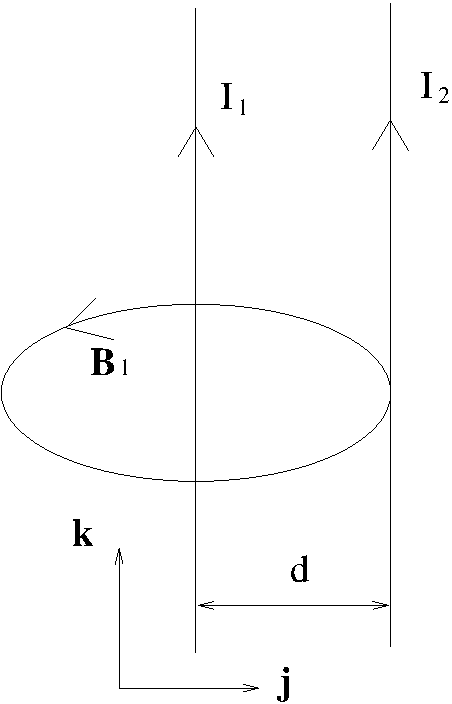
\includegraphics[scale=0.5]{immagini/fisica2/fili_forza}
\end{figure}

Usiamo Biot--Savart, il campo generato dal primo filo a distanza $d$:
\begin{equation}
\ve B(d)=\frac{\mu_0}{2\pi}I_1\frac{\ver k\times\ver \jmath}{d^2}=-\frac{\mu_0}{2\pi}\frac{I_1}{d}\ver \imath
\end{equation}
La forza sul secondo:
\begin{equation}
\label{pre_ampere}
\ud \ve F=I_2\ud\ve l_2\times\ve B(d)=-\frac{\mu_0}{2\pi}\frac{I_1}{d}I_2\ud l_2\left(\ver k\times\ver \imath\right)=-\frac{\mu_0}{2\pi}\frac{I_1I_2}{d}\ud l_2\ver \jmath
\end{equation}
Integrando:
\[\ve F=-\frac{\mu_0}{2\pi}\frac{I_1I_2}{d}l\ver \jmath\]
Se la corrente fosse stata di verso opposto allora la forza sarebbe stata repulsiva.
\subsubsection{Definizione di ampere\index{ampere}}
Dalla \eqref{pre_ampere} possiamo dire:
\begin{equation}
\frac{\ud F}{\ud l}=\frac{\mu_0}{2\pi}\frac{I_1I_2}{d}
\end{equation}
e definire l'ampere usando solo quantità meccaniche come la forza e la distanza:
\begin{Def}[ampere]
l'ampere è quella corrente che passando tra due fili distanti $\si{1}{\meter}$ produce una forza per unità di lunghezza pari a \si{2E-7}{\newton\per\meter}.
\end{Def}

\section{Circuitazione\index{circuitazione!del campo magnetico}}
Prendiamo un filo rettilineo, calcoliamo la circuitazione di $\ve B$ lungo una linea di forza:
\[\oint\ve B\cdot\ud\ve l=\oint B\,\ud l=\oint\frac{\mu_0}{2\pi}\frac{I}{R}\,\ud l=\frac{\mu_0}{2\pi}\frac{I}{R}2\pi R=\mu_0 I\]
Questo risultato vale per qualsiasi percorso purché concateni una corrente $I$. Consideriamo un circuito che non concatena nessuna corrente:
\[\int_1\ve B\cdot\ud \ve l=0\qquad\int_3\ve B\cdot\ud \ve l=0\]
\[\int_2\ve B\cdot\ud \ve l=\frac{\mu_0}{2\pi}\frac{I}{r_2}(r_2\theta)\qquad
\int_4\ve B\cdot\ud \ve l=-\frac{\mu_0}{2\pi}\frac{I}{r_1}(r_1\theta)\]
Sommando si ottiene che la circuitazione è nulla. Generalizzando si arriva al teorema di Ampere:
\begin{Teo}[Ampere\index{teorema!di Ampere}]
Sia $I$ la corrente totale che il percorso $C$ concatena:
\begin{equation}
\oint_C \ve B\cdot\ud \ve l=\mu_0I
\label{circ_ampere}
\end{equation}
se la corrente viene concatenata $n$ volte va contata $n$ volte. La corrente va contata con segno, dipendente dal verso di concatenamento, positiva se in senso antiorario.
\end{Teo}
La circuitazione dipende dal cammino della circuitazione, infatti $\ve B$ non è un campo conservativo.
\subsection{Forma differenziale}
Essendo:
\[I=\int_S\ve J\cdot\ve n\,\ud a\]
sostituendola nella \eqref{circ_ampere} si ha:
\[\oint_C \ve B\cdot\ud \ve l=\mu_0\int_S\ve J\cdot\ve n\,\ud a\]
Usando il teorema del rotore:
\[\int_S\rot\ve B\cdot\ve n\,\ud a=\mu_0\int_S\ve J\cdot\ve n\,\ud a\]
Essendo $S$ qualsiasi:
\begin{equation}
\rot\ve B=\mu_0\ve J
\end{equation}
\begin{Es}[cilindro rotante]
Sia un cilindro rotante lungo l'asse con periodo $T$, all'interno del quale ci sia una distribuzione di carica uniforme $\rho$. Vogliamo conoscere il campo magnetico generato. Per la simmetria il campo è coassiale. Creiamo un percorso che concatena parzialmente il cilindro.
\begin{figure}[htbp]
\centering
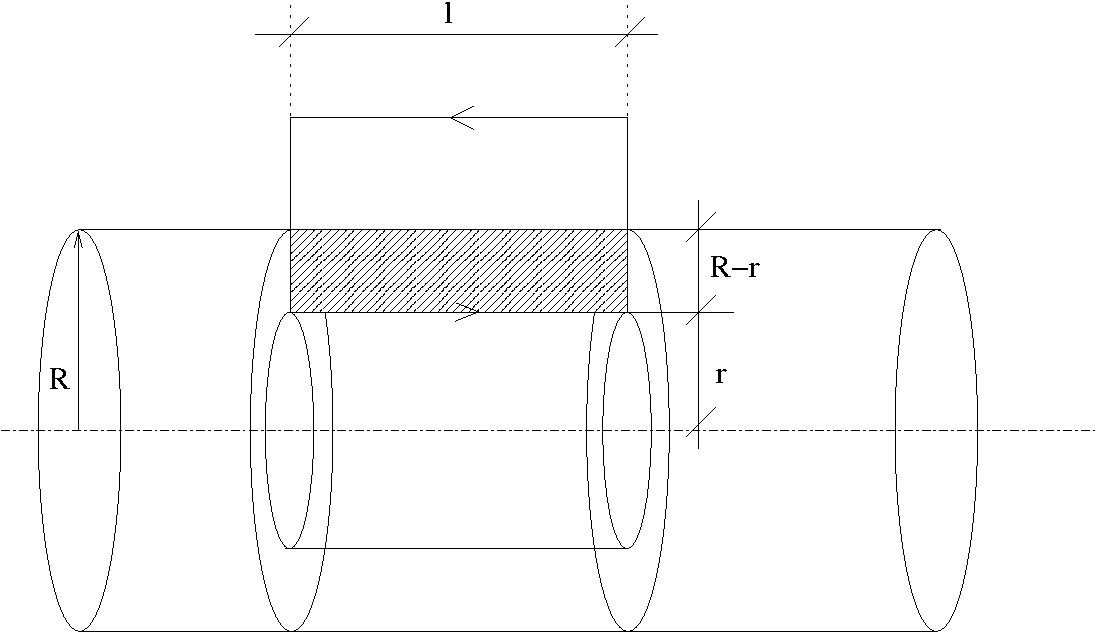
\includegraphics[scale=0.4]{immagini/fisica2/cilindro_magnetico}
\end{figure}
\[I=\frac{Q}{T}=\frac{\int_V \rho\,\ud v}{T}=\frac{\rho l\pi\left(R^2-r^2\right)}{T}\]
Per il teorema di Ampere:
\[\oint_C \ve B\cdot\ud\ve l=Bl=\mu_0 I=\mu_0\frac{\rho l\pi\left(R^2-r^2\right)}{T}\]
\[B=\mu_0\frac{\rho\pi\left(R^2-r^2\right)}{T}\]
\end{Es}


\section{Flusso\index{flusso!del campo magnetico}}
Sappiamo che le linee del campo di $\ve B$ sono linee chiuse o infinite, non esistono sorgenti. Se prendiamo una superficie qualsiasi ci accorgiamo che tante linee di forza entrano, tante ne escono, quindi:
\begin{equation}
\Phi_S\left(\ve B\right)=\int_S\ve B\cdot\ve n\,\ud a=0
\end{equation}
\subsection{Forma differenziale}
In forma differenziale:
\begin{equation}
\diver\ve B=0
\end{equation}
Questa espressione poteva essere ricavata calcolando:
\[\diver\ve B=\diver \left\{\frac{\mu_0}{4\pi}\int\frac{\ve J\left(\ve r\,'\right)\times\left(\ve r-\ve r\,'\right)}{\norm{\ve r-\ve r\,'}^3}\,\ud v'\right\}=0\]
%\begin{align*}
%\ve\nabla\cdot\ve B &= \frac{\mu_0}{4\pi}\int\ve\nabla\cdot\frac{\ve J\left(\ve r\,'\right)\times\left(\ve %r-\ve r\,'\right)}{\norm{\ve r-\ve r\,'}^3}\,\ud v'\\
%&=
%\end{align*}
\section{Maxwell per la magnetostatica}
\begin{gather}
\ve\nabla\cdot\ve B=0\\
\ve\nabla\times\ve B=\mu_0 J
\end{gather}
o in forma integrale:
\begin{gather}
\int_S\ve B\cdot\ve n\,\ud a=0\\
\int_C\ve B\cdot\ud \ve l=\mu_0 I
\end{gather}
\section{Potenziale scalare magnetico}
Supponiamo di poter scrivere:
\begin{equation}
\ve B(\ve r)=-\mu_0\grad\varphi_m(\ve r)
\label{potenziale_magnetico01}
\end{equation}
Consideriamo una spira $C$ piana percorsa da corrente $I$. La \eqref{campo_spira_laplace} ci fornisce il campo magnetico in $P$:
\begin{equation}
\ve B\left(\ve r\right)=\frac{\mu_0}{4\pi}I\oint_C\frac{\ud\ve l\times\left(\ve r-\ve r\,'\right)}{\norm{\ve r-\ve r\,'}^3}
\label{campo_spira_laplace02}
\end{equation}
Se da $P$ ci spostiamo di uno spostamento infinitesimo $\ud\ve s$ allora il potenziale in $P$ varia di:
\begin{equation}
\ud\varphi_m=\grad\varphi_m\cdot\ud \ve s=-\frac{1}{\mu_0}\ve B\cdot\ud \ve s
\end{equation}
avendo usato la \eqref{potenziale_magnetico01}. Sostituendo l'espressione del campo magnetico \eqref{campo_spira_laplace02}:
\begin{equation}
\ud\varphi_m=-\frac{I}{4\pi}\oint_C\frac{\ud \ve s\cdot(\ud\ve l\times\ve r)}{r^3}
\end{equation}
dove abbiamo battezzato $\ve r:=(\ve r-\ve r\,')$ che quindi indica il vettore che individua $P$ rispetto a $\ud\ve l$. L'ultima relazione la possiamo anche scrivere come:
\begin{equation}
\ud\varphi_m=-\frac{I}{4\pi}\oint_C\frac{\ve r\cdot(\ud \ve s\times\ud\ve l)}{r^3}
\label{variazione_campo_magnetico02}
\end{equation}
Tutto ciò lo possiamo ottenere mantenendo $P$ fermo e spostando la spira di $-\ud\ve s$ e la variazione del campo magnetico sarebbe ancora \eqref{variazione_campo_magnetico02}. Durante questo spostamento i vettori $\ud\ve l$ e $\ud \ve s$ descrivono un'area $\ud \ve a=-\ud\ve s\times\ud\ve l$ che compare nella \eqref{variazione_campo_magnetico02} e punta nel semispazio di $P$. Vogliamo dimostrare che l'integrale:
\[
-\oint_C\frac{\ve r\cdot(\ud \ve s\times\ud\ve l)}{r^3}
\]
è uguale a $\ud\omega$, la variazione di $\omega$, l'angolo solido con cui $P$ vede $C$, durante lo spostamento $\ud\ve s$. $\ud \ve a\cdot\ve r=\ud a_0 r$ area perpendicolare a $\ve r$:
\[\frac{\ve r\cdot\ud\ve a}{r^3}=\frac{r\ud a_0}{r^3}=\frac{\ud a_0}{r^2}=\ud\ud\omega\]
integrando si trova $\ud\omega$. Allora:
\begin{equation}
\ud\varphi_m=\frac{I}{4\pi}\ud\omega
\end{equation}
e quindi:
\begin{equation}
\varphi_m=\frac{I\omega}{4\pi}
\label{potenziale_magnetico_03}
\end{equation}

Suddividiamo la superficie $S$ delimitata da $C$ in tante spire di area $\ud a$ percorse da corrente $I$. Per il solito discorso sommando tutte le $\ud a$ si torna alla spira $C$. Il verso della corrente determina l'orientamento delle spire. Essendo:
\[\omega=\int_S\frac{\ud\ve a\cdot\ve r}{r^3}\]
possiamo scrivere la \eqref{potenziale_magnetico_03} come:
\begin{equation}
\varphi_m=\frac{1}{4\pi}\int_S\frac{I\ud\ve a\cdot\ve r}{r^3}
\label{potenziale_magnetico_04}
\end{equation}
essendo il momento della spira elementare $\ud\ve m=I\ud a\ve n=I\ud\ve a$ lo possiamo introdurre nella \eqref{potenziale_magnetico_04}:
\begin{equation}
\varphi_m=\frac{1}{4\pi}\int_S\frac{\ud\ve m\cdot\ve r}{r^3}
\end{equation}
Sviluppando a grande distanza il potenziale è approssimato da:
\begin{equation}
\varphi_m(\ve r)=\frac{\ve m\cdot\ve r}{4\pi r^3}
\end{equation}
con $\ve m=IS\ve n$. Tornando alla notazione iniziale:
\begin{equation}
\varphi_m(\ve r)=\frac{1}{4\pi}\frac{\ve m\cdot\left(\ve r-\ve r\,'\right)}{\norm{\ve r-\ve r\,'}^3}=-\frac{1}{\mu_0}\int_\infty^{\ve r}\ve B\cdot\ud\ve l
\end{equation}

\section{Potenziale vettoriale magnetico\index{potenziale!vettoriale!magnetico}}
Essendo la divergenza del vettore $\ve B$ nulla, cioè essendo $\ve B$ un campo vettoriale solenoidale si può dimostrare che:
\begin{equation}
\exists\ve A:\ve B=\rot\ve A
\label{vet_magnetico00}
\end{equation}
in questo caso $\ve A$ è detto potenziale vettore magnetico, e non è univocamente determinato, per esempio se scegliamo un certo $\ve A$ potenziale vettore allora anche $\ve A+\grad\psi$ soddisfa la condizione \eqref{vet_magnetico00}:
\[
\rot\left(\ve A+\grad\psi\right)=\rot\ve A
\]
in quando il rotore di un gradiente è sempre nullo. Tra le tante possibili scelte di $\ve A$ scegliamo (per la magnetostatica) $\ve A$ tale che:
\begin{equation}
\diver\ve A=0
\label{gauge_magnetos}
\end{equation}
questo è sempre possibile, supponiamo che $\diver\ve A=k\neq 0$, ma allora scelgo $\ve A'=\ve A +\grad\psi$ tale che $\nabla^2\psi = -k$, allora $\diver \ve A'=0$. Sappiamo dalla circuitazione di Ampere che:
\begin{equation}
\rot\ve B=\mu_0\ve J
\end{equation}
Sostituendo la \eqref{vet_magnetico00}:
\begin{equation}
\rot\ve B=\rot\rot\ve A=\grad\diver\ve A-\nabla^2\ve A=\mu_0\ve J
\end{equation}
e per la condizione per la magnetostatica \eqref{gauge_magnetos}:
\begin{equation}
\nabla^2\ve A=-\mu_0\ve J
\label{gauge_magnetos1}
\end{equation}
da confrontare con la \eqref{Poisson01} per l'elettrostatica $\nabla^2\varphi = -\frac{\rho}{\epsilon_0}$, che però è un equazione scalare. La soluzione della \eqref{gauge_magnetos1} è 
\begin{equation}
\ve A(\ve r)=\frac{\mu_0}{4\pi}\int_V\frac{\ve J(\ve r\,')}{\norm{\ve r-\ve r\,'}}\,\ud v'
\label{vet_magnetico01}
\end{equation}
\subsection{Dipolo magnetico\label{dipolo!magnetico}}
\begin{figure}[htbp]
\centering
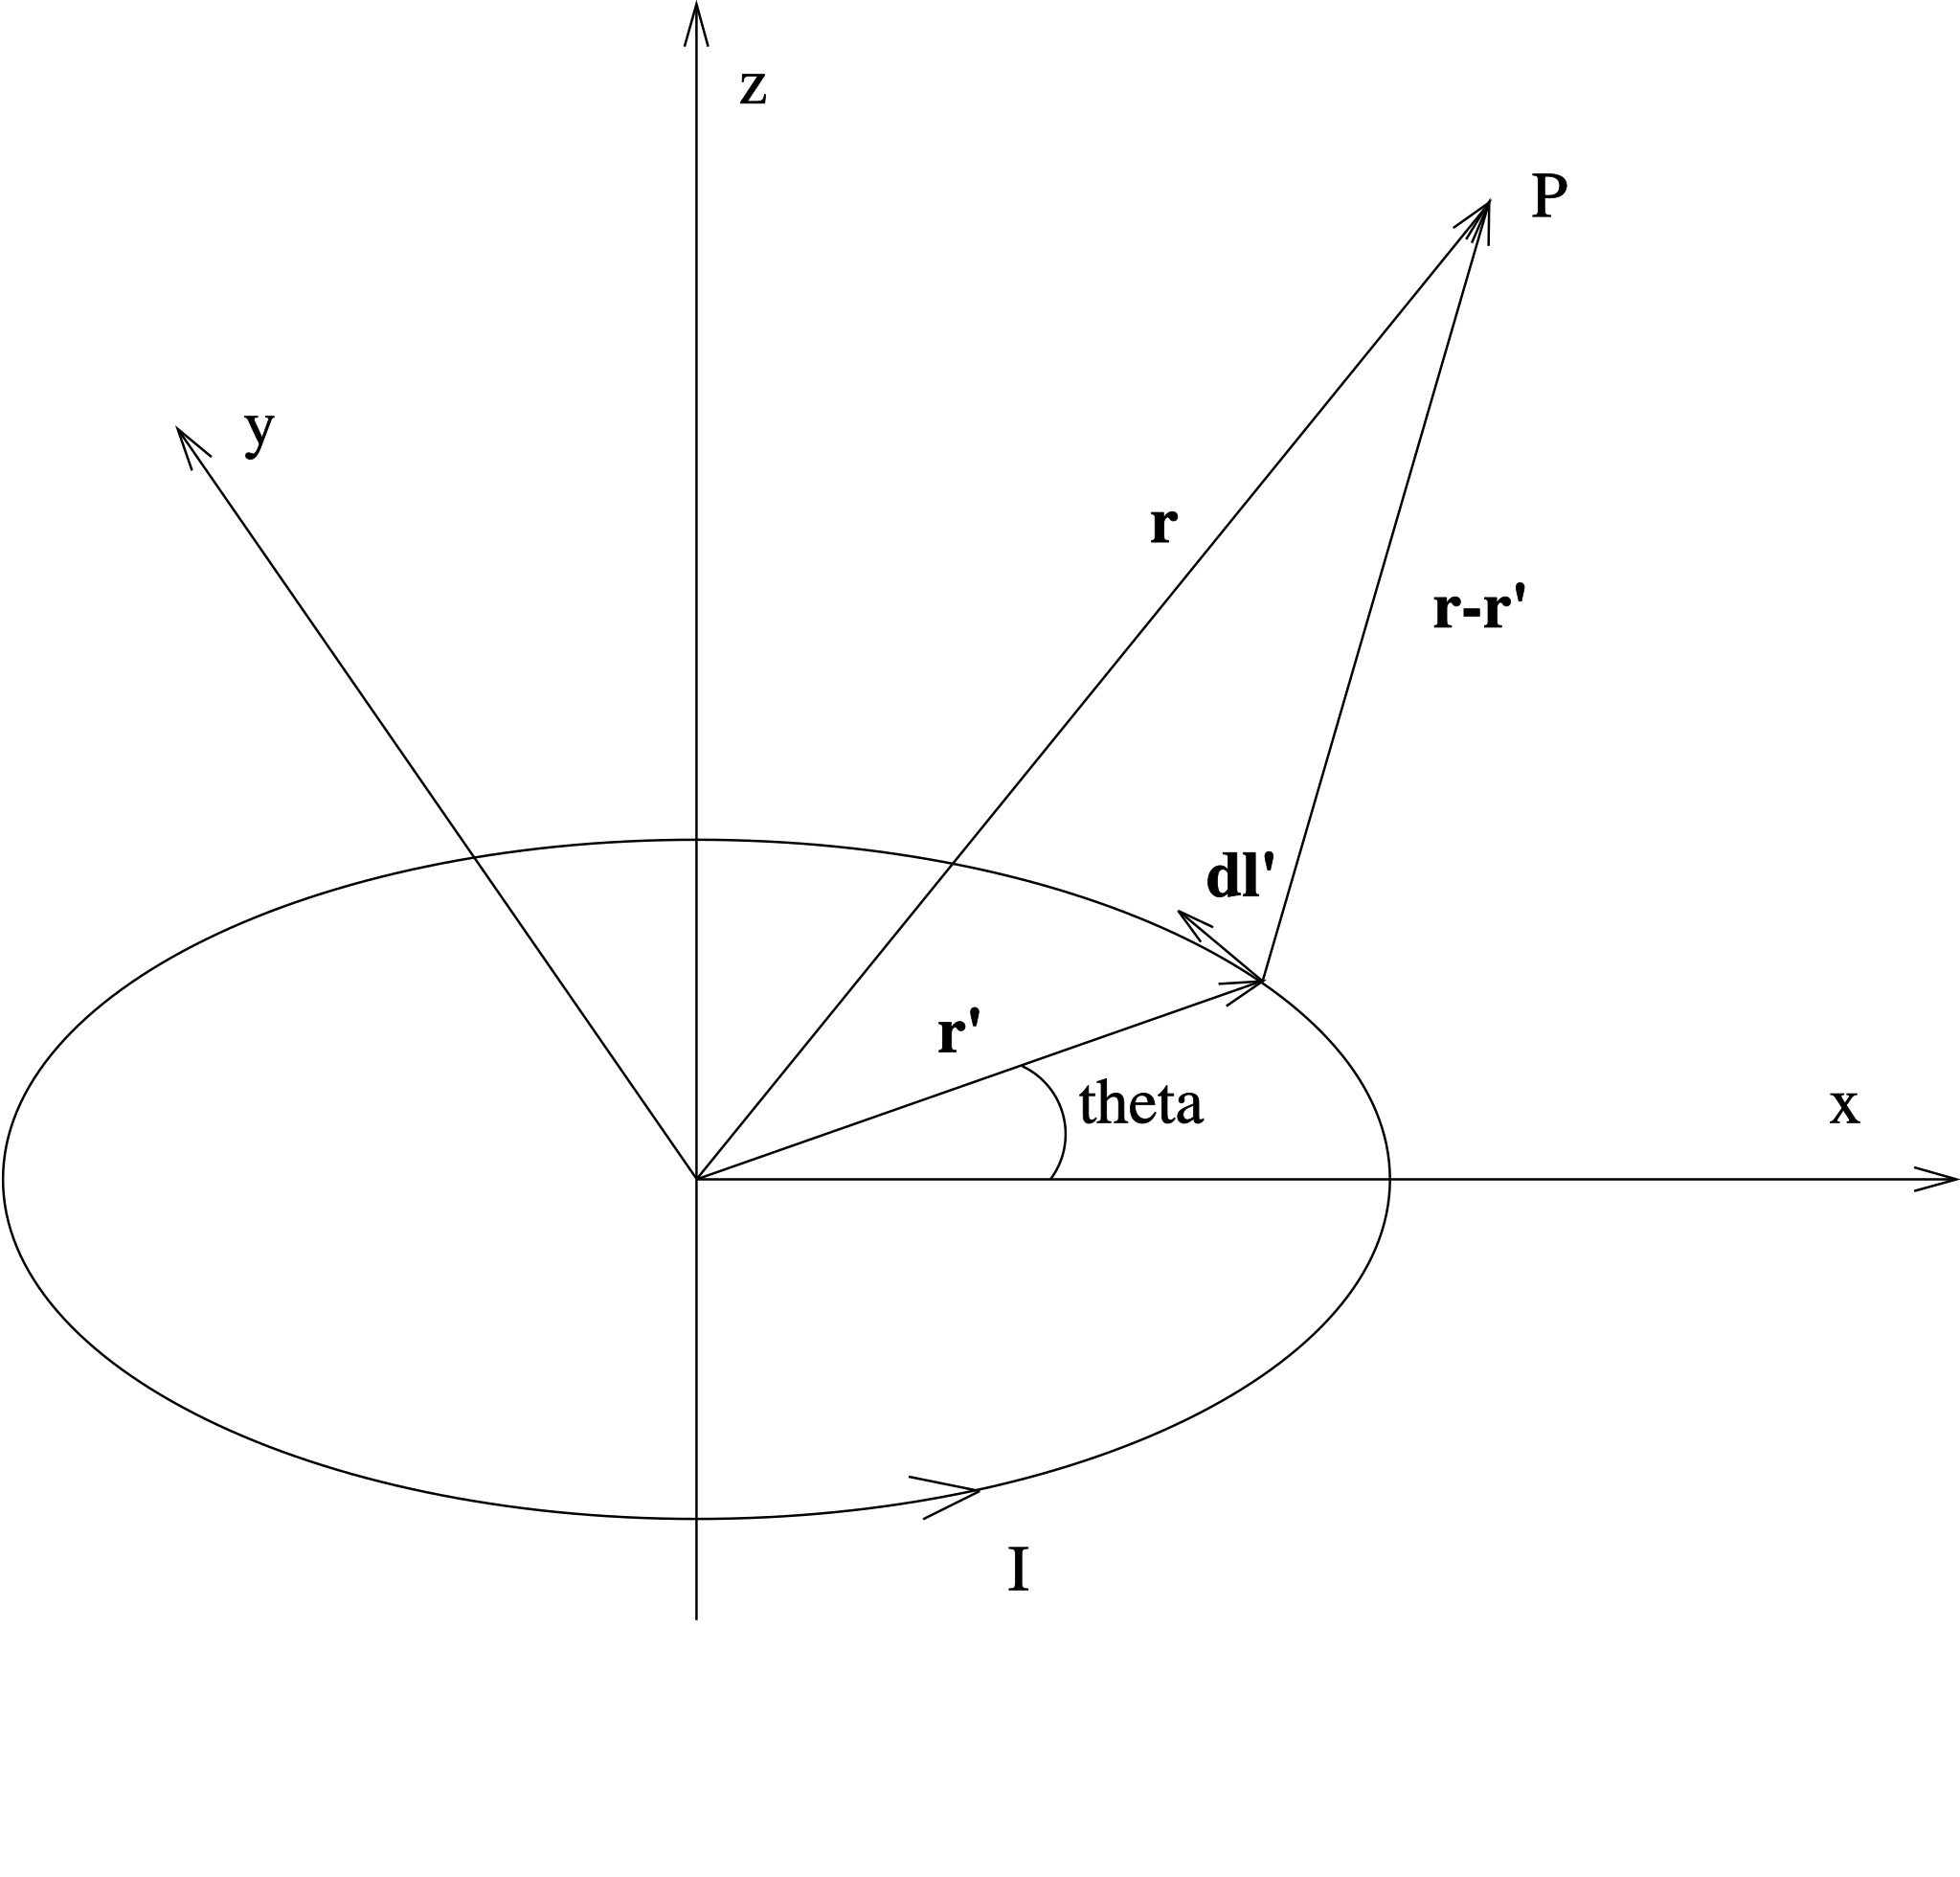
\includegraphics[scale=0.5]{immagini/fisica2/spira_vettore}
\end{figure}
Calcoliamo il potenziale vettoriale generato da una spira circolare di raggio $r'$ percorsa da corrente stazionaria $I$. Dalla \eqref{vet_magnetico01}:
\begin{equation}
\ve A(\ve r)=\frac{\mu_0}{4\pi}I\oint\frac{\ud \ve l'}{\norm{\ve r-\ve r\,'}}
\label{dipolo_magnetico01}
\end{equation}
essendo $\ve J\,\ud v'=I\ud\ve l'$. Se la spira giace nel piano $xy$ allora la componente $\ve A_z$ è nulla essendo $\ud \ve l\,'$ nel piano $xy$. Introducendo il momento magnetico della spira:
\begin{equation}
\ve m=IA\ve n
\end{equation}
con $A$ l'area della superficie racchiusa dalla spira, possiamo descrivere la spira come un dipolo magnetico mediante il potenziale vettoriale, sviluppando la \eqref{dipolo_magnetico01}. Sappiamo già che se usassimo il potenziale scalare magnetico potremmo scrivere:
\begin{equation}
\varphi_m=\frac{1}{4\pi}\frac{\ve m\cdot\ve r}{r^3}
\end{equation}
sviluppiamo la quantità $\norm{\ve r-\ve r'}^{-1}$ che compare nella \eqref{dipolo_magnetico01}:
\[
\norm{\ve r-\ve r'}^{-1}=\left(\ve r^2+\ve r'^2-2\ve r\cdot \ve r'^2\right)^{-\frac{1}{2}}=\frac{1}{r}\left(1+\frac{r'^2}{r^2}-\frac{2\ve r\cdot\ve r'}{r^2}\right)^{-\frac{1}{2}}
\]
Consideriamo $r\gg r'$, consideriamo solo i termini del primo ordine dello sviluppo di potenze:
\begin{equation}
\begin{aligned}
\norm{\ve r-\ve r'}^{-1}&=\frac{1}{r}\left(1-\frac{1}{2}\frac{r'^2}{r^2}+\frac{\ve r\cdot\ve r'}{r^2}+o\left(\frac{r'^2}{r^2}+2\frac{\ve r\cdot\ve r'}{r^2}\right)\right)\\
&=\frac{1}{r}\left(1+\frac{\ve r\cdot \ve r'}{r^2}+o\left(\frac{r'}{r}\right)\right)\simeq\frac{1}{r}\left(1+\frac{\ve r\cdot \ve r'}{r^2}\right)
\end{aligned}
\end{equation}
Tenendo conto che:
\begin{equation}
 \ud \ve l'=r'\ud\theta\ver u_\theta \qquad \ve r' = r'\ver u_r
\end{equation}
Allora la \eqref{dipolo_magnetico01} si scrive come:
\begin{equation}
 \begin{aligned}
  \ve A &= \frac{\mu_0}{4\pi}\frac{I}{r}\oint \ud\ve l'\cdot\left(1+\frac{\ve r'\cdot \ve r}{r^2}\right)\\
        &= \frac{\mu_0}{4\pi}\frac{I}{r^3}\oint \ud\ve l'\cdot(\ve r'\cdot \ve r)\\
	&= \frac{\mu_0}{4\pi}\frac{I}{r^3}r'^2\oint \ver u_\theta(\cos\theta x+\sin\theta y)\,\ud\theta
 \end{aligned}
\end{equation}
ricordando che $\ver u_r = \cos\theta\ver i+\sin\theta\ver j$ e $\ver u_\theta = -\sin\theta\ver i+\cos\theta\ver j$ le componenti di $\ve A$:
\begin{equation*}
 \begin{aligned}
  A_x &= \frac{\mu_0}{4\pi}\frac{I}{r^3}r'^2\int_0^{2\pi}-\sin\theta(\cos\theta x+\sin\theta y)\,\ud\theta=-\frac{\mu_0}{4\pi}\frac{I}{r^3}r'^2\pi y\\
  A_y &= \frac{\mu_0}{4\pi}\frac{I}{r^3}r'^2\int_0^{2\pi}-\cos\theta(\cos\theta x+\sin\theta y)\,\ud\theta=\frac{\mu_0}{4\pi}\frac{I}{r^3}r'^2\pi x\\
 \end{aligned}
\end{equation*}
che si riassume, tenendo conto che l'area è $A=\pi r'^2$:
\begin{equation}
\ve A=\frac{\mu_0}{4\pi}\frac{\ve m\times\ve r}{r^3}
\end{equation}


\chapter{Dielettrici\index{dielettrici}}
\minitoc
Se vogliamo calcolare esattamente il campo elettrico a livello microscopico \index{campo!elettrico!microscopico}$\ve\varepsilon$ all'interno della materia quello che dovremo conoscere è la distribuzione di carica microscopica. Questa distribuzione di carica è generata dagli elettroni e dai protoni. La soluzione delle equazioni di Maxwell per l'elettrostatica è:
\begin{equation}
 \ve\varepsilon(\ve x) = \frac{1}{\giorgi}\int \rho(\ve x')\frac{\ve x -\ve x'}{\norm{\ve x-\ve x'}^3}\,\ud V'
\end{equation}
questa soluzione non è molto utile, in quanto $\rho$ dovrebbe essere conosciuta con precisione a livello microscopico ed è la sovrapposizione di moltissime particelle; inoltre il risultato $\ve\varepsilon$ varierebbe molto velocemente su scala microscopica. Per un'analisi macroscopica non abbiamo bisogno di questa precisione, e quindi possiamo lavorare con una $\rho$ e una $\ve\varepsilon$ mediata.

\section{Isolanti\index{isolanti}}
A differenza che nei conduttori negli isolanti o dielettrici gli elettroni sono fortemente legati ai nuclei e non si possono allontanare. Su di essi però agisce una forza $\ve F=-e\ve E_0$ se sottoposti ad un campo elettrico esterno $\ve E_0$. Non si parla di moto di cariche, ma di spostamento. Gli elettroni spostandosi dalla loro posizione originaria fanno si che il centro di carica positiva e negativa non coincidano più. Il dielettrico si dice polarizzato e il fenomeno è chiamato polarizzazione\index{polarizzazione}. In questo modo si crea un campo elettrico di polarizzazione $\ve E_P$; il campo elettrico totale:
\begin{equation}
\ve E_T=\ve E_0+\ve E_P
\end{equation}
ma $\ve E_P=\ve E_P(\ve E_T)$.

Consideriamo un approccio fenomenologico. Consideriamo un condensatore a facce piane e parallele. La sua capacità è $C_0=\varepsilon_0\frac{S}{d}$. Se sulle armature depositiamo una carica $q$ si creerà una differenza di potenziale $\Delta V_0=E_0d=\frac{\sigma}{\varepsilon_0}d$. Inseriamo un dielettrico tra le armature, si nota che la capacità è aumentata di un fattore $\varepsilon_r>1$:
\[C=\varepsilon_rC_0\]
$\varepsilon_r$ è caratteristica del dielettrico. $\Delta V$ è diminuita:
\[\Delta V=\frac{Q}{C}=\frac{Q}{\varepsilon_r C_0}=\frac{\Delta V_0}{\varepsilon_r}\]
anche il campo è diminuito:
\[E=\frac{\Delta V}{d}=\frac{\Delta V_0}{\varepsilon_rd}=\frac{E_0}{\varepsilon_r}\]
allora la forza:
\[F=qE=\frac{qE_0}{\varepsilon_r}\]
La legge di Coulomb nei dielettrici diventa:
\begin{equation}
\ve F=\frac{q}{4\pi\varepsilon_0\varepsilon_r}\frac{\ve r-\ve r\,'}{{\norm{\ve r-\ve r\,'}}^3}
\end{equation}
Per usarla anche nel vuoto $\varepsilon_r=1$ nel vuoto. Mentre la circuitazione è sempre nulla il teorema di Gauss\index{teorema!di Gauss!nei dielettrici} diventa:
\begin{subequations}
\begin{gather}
\oint_S\ve E\cdot\ve n\,\ud a=\frac{Q}{\varepsilon_0\varepsilon_r}\\
\ve\nabla\cdot\ve E=\frac{\rho}{\varepsilon_0\varepsilon_r}
\end{gather}
\end{subequations}
\section{Polarizzazione\index{polarizzazione}}
Ogni molecola del dielettrico è considerata neutra. Il termine successivo dello sviluppo in multipoli è quello del dipolo:
\begin{equation}
\varphi(\ve r)=\frac{1}{4\pi\varepsilon_0}\frac{\ve r}{r^3}\cdot\int_V\ve r\,'\rho(\ve r\,')\,\ud v'
\end{equation}
e lo scriviamo come:
\begin{equation}
\varphi(\ve r)=\frac{1}{4\pi\varepsilon_0}\frac{\ve p\cdot\ve r}{r^3}
\end{equation}
con
\begin{equation}
\ve p=\int_V \ve r\,'\rho(\ve r\,')\,\ud v
\end{equation}
momento di dipolo. Se invece prendiamo un'origine generica, non al centro del dipolo:
\begin{equation}
\varphi(\ve r)=\frac{1}{4\pi\varepsilon_0}\frac{\ve p\cdot\left(\ve r-\ve r\,'\right)}{\norm{\ve r-\ve r\,'}^3}
\label{dipolo_scentrato}
\end{equation}
\begin{equation}
\ve E=\frac{1}{4\pi\varepsilon_0}\left[\frac{3\left(\ve p\cdot\left(\ve r-\ve r\,'\right)\right)\left(\ve r-\ve r\,'\right)}{{\norm{\ve r-\ve r\,'}}^5}-\frac{\ve p}{{\norm{\ve r-\ve r\,'}}^3}\right]
\end{equation}
Consideriamo le nostre molecole polarizzate come dei dipoli, e il dielettrico come somma di tanti dipoli. Possiamo vedere anche il dielettrico come un unico dipolo, risultante dalla somma, è come se concentrassimo della carica $\Delta q$ in un volumetto $\Delta V$ e della carica $-\Delta q$ in un altro volumetto uguale a distanza $\delta$ tale che $\ve p=|\Delta q|\ve\delta$.
\begin{figure}[htbp]
\centering
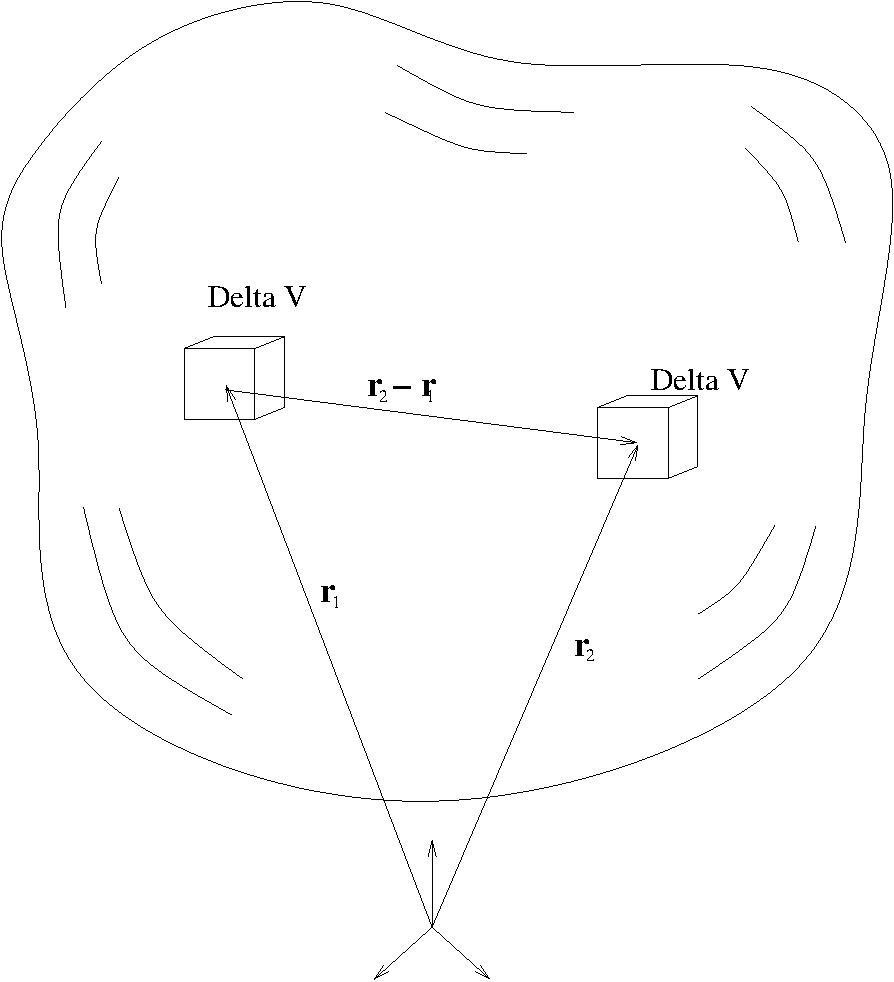
\includegraphics[scale=0.3]{immagini/fisica2/distr_dipoli}
\end{figure}
\subsection{Momento atomico\index{momento!atomico}}
Il modello atomico più semplice è quello di Bohr\index{Bohr}\index{modello!di Bohr}. Consideriamo l'atomo di idrogeno. Al centro troviamo un nucleo positivo e un elettrone negativo che gira attorno a distanza $a\simeq \si{0.5}{\angstrom}$. L'atomo è un momento di dipolo $\ve p=e\ve a$ che ruota. Mediamente esso è nullo.

Se consideriamo la meccanica quantistica attorno al nucleo l'elettrone assomiglia a una distribuzione negativa di raggio $a$. Essendo la distribuzione a simmetria sferica, tutti gli atomi non sottoposti a campi elettrici non hanno momento di dipolo essendo i centri di cariche positive e negative coincidenti.
\subsection{Molecole polari\index{molecole!polari}\index{molecole!polari}}
A seconda della composizione e anche della geometria che ne deriva le molecole possono essere polari o apolari. Per esempio O$_2$, H$_2$, CO$_2$ sono apolari, mentre H$_2$O, HCl, NaCl presentano un momento di dipolo.

Se consideriamo un campione abbastanza numeroso di molecole polari la media dei momenti di dipolo sarà nulla, essendo l'orientazione dei singoli dipoli casuale.
\subsection{Polarizzazione per orientamento\index{polarizzazione!per orientamento}}
Un campo elettrico esterno su una molecola polare tenderà ad orientare il suo momento di dipolo parallelamente al campo. Questo non vuol dire che tutte le molecole sono orientate siano orientate parallelamente al campo elettrico, in quanto il movimento che prevale è quello di agitazione termica, che mediamente è nullo. Se lo eliminiamo vedremo i momenti di dipolo che oscillano attorno alla direzione parallela al campo elettrico esterno. In generale si noterà che ogni singolo dipolo avrà mediamente una componente non nulla nella direzione del campo elettrico. La molecola è polarizzata per orientamento.
\subsection{Polarizzazione per deformazione\index{polarizzazione!per deformazione}}
Se mettiamo un atomo, o una molecola apolare, in un campo elettrico risulterà deformato: il centro di carica positiva e negativa non coincideranno più, si è creato un momento di dipolo indotto\index{momento!di dipolo!indotto}, il dielettrico è polarizzato per deformazione. Anche le molecole polari subiscono questo effetto, ma è di gran lunga inferiore alla polarizzazione per orientamento.
\subsection{Vettore polarizzazione elettrica}
Consideriamo un elemento $\Delta V$ di un dielettrico polarizzato. Questo presenterà un momento di dipolo:
\[
\Delta\ve p=\int_{\Delta V}\rho(\ve r)\ve r\,\ud v=\int_{\Delta V}\ve r\,\ud q
\]
\begin{Def}[vettore polarizzazione elettrica\index{vettore!polarizzazione!elettrica}]
\begin{equation}
\ve P(\ve r)=\frac{\Delta\ve p(\ve r)}{\Delta V}
\label{vettore_polarizzazione_elettrica}
\end{equation}
con $\Delta V$ si intende un elemento di volume sufficientemente piccolo da un punto di vista macroscopico in modo che $\ve P$ possa essere assunto uniforme all'interno di $\Delta V$, da un punto di vista microscopico abbastanza grande per contenere abbastanza atomi da variare con continuità.
\end{Def}
$\ve P$ è dato dalla somma di tutti i momenti di dipolo delle singole molecole:
\begin{equation}
\ve P=\frac{\sum\ve p_m}{\Delta V}
\end{equation}
Se non c'è un campo elettrico esterno allora $\ve P=0$ anche se $\ve p_m\neq 0$ nelle molecole polari, in quanto sono orientate in modo casuale. In realtà esistono materiali, detti elettreti\index{elettreti} che mantengono $\ve P$ anche dopo una polarizzazione in assenza di campo elettrico.

Anche nei conduttori avviene l'effetto di polarizzazione, ma è trascurabile.

\section{Campo elettrico generato da un dielettrico\index{campo!elettrico!di un dielettrico}}
\label{section:Campo_elettrico_generato_da_un_dielettrico}
\subsection{Esterno}
Consideriamo un dielettrico polarizzato, vogliamo calcolare il campo elettrico da esso generato all'esterno del dielettrico conoscendo il vettore $\ve P(\ve r)$. Consideriamo un elementino $\ud v'$ individuato dal vettore $\ve r\,'$. Esso presenta un momento di dipolo $\ud\ve p=\ve P(\ve r\,')\ud v'$ per la \eqref{vettore_polarizzazione_elettrica}. Segue dall'espressione del potenziale del dipolo \eqref{dipolo_scentrato} che l'elementino $\ud v'$ genera un potenziale:
\begin{equation}
\ud\varphi(\ve r)=\frac{1}{4\pi\varepsilon_0}\frac{\ve P(\ve r\,')\cdot\left(\ve r-\ve r\,'\right)}{\norm{\ve r-\ve r\,'}^3}\ud v'
\end{equation}
Il potenziale generato da tutto il dielettrico di volume $V$ sarà 
\begin{equation}
\varphi(\ve r)=\int_V\ud\varphi(\ve r)=\frac{1}{4\pi\varepsilon_0}\int_V\frac{\ve P(\ve r\,')\cdot\left(\ve r-\ve r\,'\right)}{\norm{\ve r-\ve r\,'}^3}\ud v'
\label{potenziale_dielettrico03}
\end{equation}
Possiamo introdurre il gradiente, rispetto alle coordinate primate, usando la relazione:
\begin{equation}
\ve\nabla'\frac{1}{\norm{\ve r-\ve r\,'}}=\frac{\left(\ve r-\ve r\,'\right)}{\norm{\ve r-\ve r\,'}^3}
\end{equation}
Possiamo allora riscrivere l'ultima equazione \eqref{potenziale_dielettrico03}:
\begin{equation}
\varphi(\ve r)=\frac{1}{4\pi\varepsilon_0}\int_V\ve P(\ve r\,')\cdot\ve\nabla'\frac{1}{\norm{\ve r-\ve r\,'}}\ud v'
\label{potenziale_dielettrico04}
\end{equation}
Usando la relazione:
\begin{equation}
\ve\nabla\cdot(f\ve F)=f\ve\nabla\cdot\ve F+\ve F\cdot\ve\nabla f
\end{equation}
con $f$ una funzione scalare e $\ve F$ una vettoriale. Considerando $\ve F=\ve P(\ve r\,')$ e $f=\frac{1}{\norm{\ve r-\ve r\,'}}$ si ha:
\begin{equation}
\ve P(\ve r\,')\cdot\ve\nabla'\frac{1}{\norm{\ve r-\ve r\,'}}=\ve\nabla'\cdot\frac{\ve P(\ve r\,')}{\norm{\ve r-\ve r\,'}}-\frac{\ve\nabla'\cdot\ve P(\ve r\,')}{\norm{\ve r-\ve r\,'}}
\end{equation}
La \eqref{potenziale_dielettrico04} diventa:
\begin{equation}
\varphi(\ve r)=\frac{1}{4\pi\varepsilon_0}\left[\int_V\ve\nabla'\cdot\frac{\ve P(\ve r\,')}{\norm{\ve r-\ve r\,'}}\ud v'-\int_V\frac{\ve\nabla'\cdot\ve P(\ve r\,')}{\norm{\ve r-\ve r\,'}}\ud v'\right]
\end{equation}
Usando il teorema della divergenza:
\begin{equation}
\varphi(\ve r)=\frac{1}{4\pi\varepsilon_0}\left[\int_S\frac{\ve P(\ve r\,')\cdot \ve n}{\norm{\ve r-\ve r\,'}}\ud a'+\int_V\frac{-\ve\nabla'\cdot\ve P(\ve r\,')}{\norm{\ve r-\ve r\,'}}\ud v'\right]
\end{equation}
$\ve P\cdot\ve n$ ha le dimensioni di una distribuzione superficiale di carica, mentre $-\nabla'\cdot\ve P$ ha le dimensioni di una distribuzione di carica volumetrica.
\begin{subequations}
\begin{gather}
\sigma_p(\ve r\,')=\ve P(\ve r\,')\cdot \ve n\\
\rho_p(\ve r\,')=-\ve\nabla'\cdot\ve P(\ve r\,')
\end{gather}
\end{subequations}
chiamate densità superficiale \index{densità superficiale!delle cariche di polarizzazione}\index{densità superficiale!delle cariche legate}e densità volumetrica \index{densità volumetrica!delle cariche di polarizzazione}\index{densità volumetrica!delle cariche legate}delle cariche di polarizzazione o legate.

In definitiva abbiamo dimostrato che il potenziale generato da un dielettrico polarizzato in un punto esterno ad esso è uguale al potenziale generato da una distribuzione di cariche superficiale $\sigma_p$ lungo il bordo e una distribuzione di cariche volumetrica $\rho_p$ all'interno del volume del dielettrico. Condizione sufficiente affinché $\rho_p=0$ è che $\ve P$ sia uniforme, infatti la divergenza si annulla\footnote{
Non è necessaria, infatti se $\ve P$ è proporzionale a $\frac{\ve r}{r^3}$ le derivate non sono nulle:
\[
\frac{\partial}{\partial x} \frac{x}{r^3}=\frac{r^3-3xr^2\frac{1}{2}\left(x^2+y^2+z^2\right)^{-\frac{1}{2}}2x}{r^6}=\frac{1}{r^3}-3\frac{x^2}{r^5}
\]
ma la divergenza si annulla:
\[
\diver\left(\frac{\ve r}{r^3}\right)=3\frac{1}{r^3}-\frac{3x^2}{r^5}-3\frac{y^2}{r^5}-\frac{3z^2}{r^5}=\frac{3}{r^3}-\frac{3}{r^3}=0
\]
}.
\begin{equation}
\varphi(\ve r)=\frac{1}{4\pi\varepsilon_0}\left[\int_S\frac{\sigma_p(\ve r\,')}{\norm{\ve r-\ve r\,'}}\ud a'+\int_V\frac{\rho_p(\ve r\,')}{\norm{\ve r-\ve r\,'}}\ud v'\right]
\label{potenziale_dielettrico_esterno9}
\end{equation}
Il dielettrico rimane sempre neutro per la conservazione della carica, infatti la carica totale di polarizzazione è 
\begin{equation}
\begin{split}
Q_P&=\int_S\sigma_p\,\ud a+\int_V\rho_P\,\ud v=\int_S\ve P\cdot\ve n\,\ud a+\int_V-\ve\nabla\cdot\ve P\,\ud v\\
&=\int_S\ve P\cdot\ve n\,\ud a-\int_S\ve P\cdot\ve n\,\ud a=0
\end{split}
\end{equation}
Calcoliamo il campo esterno generato da un dielettrico polarizzato dall'espressione del potenziale \eqref{potenziale_dielettrico_esterno9}:
\begin{equation}
\ve E(\ve r)=\frac{1}{4\pi\varepsilon_0}\int_S-\ve\nabla\left(\frac{\sigma_p(\ve r\,')}{\norm{\ve r-\ve r\,'}}\right)\,\ud a'+\frac{1}{4\pi\varepsilon_0}\int_V-\ve\nabla\left(\frac{\rho_p(\ve r\,')}{\norm{\ve r-\ve r\,'}}\right)\,\ud v'
\end{equation}
Usando:
\[
\nabla\left(\frac{1}{\norm{\ve r-\ve r\,'}}\right)=-\nabla'\left(\frac{1}{\norm{\ve r-\ve r\,'}}\right)=-\frac{\ve r-\ve r\,'}{\norm{\ve r-\ve r\,'}^3}
\]
\begin{equation}
\ve E(\ve r)=\frac{1}{4\pi\varepsilon_0}\int_S\frac{\sigma_p(\ve r\,')(\ve r-\ve r\,')}{\norm{\ve r-\ve r\,'}^3}\,\ud a'+\frac{1}{4\pi\varepsilon_0}\int_V\frac{\rho_p(\ve r\,')(\ve r-\ve r\,')}{\norm{\ve r-\ve r\,'}^3}\,\ud v'
\label{campo_elettrico_esterno_dielettrico}
\end{equation}
che è proprio il campo generato dalle distribuzioni $\sigma_p$ e $\rho_p$.
\subsection{Interno}
All'interno di un dielettrico il campo elettrico varia da punto a punto in modo complesso, bisognerebbe tenere conto di tutti gli atomi, di come sono orientati ad un certo istante\ldots Siamo invece interessati a una quantità macroscopica, cioè alla media del campo elettrico microscopico in un volume abbastanza grande per contenere un numero grande di molecole in modo che vari con continuità ma abbastanza piccolo perché vari. I procedimenti per arrivare alla definizione di campo elettrico interno sono equivalenti e sono per esempio:
\begin{enumerate}
\item{Si prende il valore medio nel tempo e nello spazio del campo elettrico effettivamente esistente definito come la forza su una carica di prova e la sua carica;}
\item{Si considera la media del campo elettrico generato da tutte le molecole polarizzate e dalle cariche libere su una singola molecola interna al dielettrico, in parole povere $\ve E=\ve E_{\text{ext}}+\frac{\ve{P}}{3\varepsilon_0}$;}
\item{Si immagina una cavità aghiforme all'interno del dielettrico in cui ci sia il vuoto. Il campo elettrico nel dielettrico sarà il campo elettrico nella cavità \index{cavità!aghiforme};}
\end{enumerate}
Anche all'interno del dielettrico deve valere:
\[
\oint_C \ve E\cdot\ud\ve l=0
\]
infatti il dielettrico può essere visto come un insieme di cariche nel vuoto ferme. Scaviamo una cavità cilindrica molto sottile, aghiforme di volume $V_0$ e superficie $S_0$ all'interno del nostro dielettrico di volume $V$ e superficie $S$ polarizzato con vettore di polarizzazione $\ve P(\ve r)$. All'interno della cavità ci sia il vuoto e la sua presenza non alteri la polarizzazione del dielettrico. Calcoliamo la circuitazione del campo elettrico lungo un circuito rettangolare con i lati maggiori paralleli all'asse del cilindro, uno all'interno della cavità l'altro fuori. Il campo all'interno della cavità sia $\ve E_0$, nel dielettrico $\ve E_d$:
\begin{figure}[htbp]
\centering
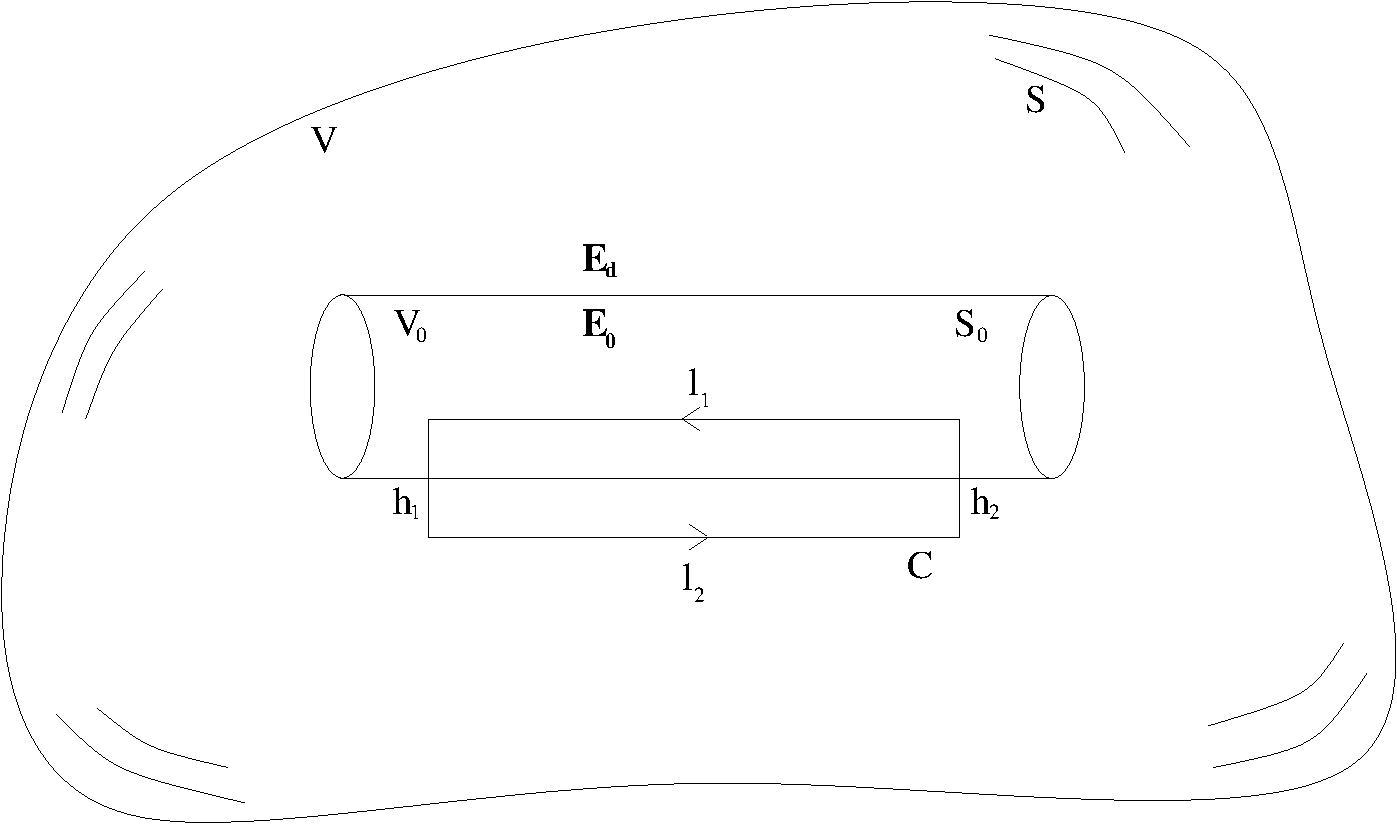
\includegraphics[scale=0.4]{immagini/fisica2/aghiforme}
\end{figure}
\begin{equation}
\int_{\Delta l_1}\ve E_0\cdot\ud\ve l+\int_{\Delta l_2}\ve E_d\cdot\ud\ve l+\int_{h_1}\ve E\cdot\ud\ve l+\int_{h_2}\ve E\cdot\ud\ve l=0
\end{equation}
Facciamo tendere $\Delta h_1$ e $\Delta h_2$ a zero, gli ultimi due integrali diventano nulli. Essendo $\ud \ve l$ parallelo all'asse del cilindro svolgiamo il prodotto scalare:
\begin{equation}
\int_{\Delta l_1}E_{0\tan}\,\ud l-\int_{\Delta l_2}E_{d\tan}\,\ud l=0
\end{equation}
Essendo $\Delta l_1$ uguale a $\Delta l_2$:
\begin{equation}
E_{0\tan}=E_{d\tan}
\label{E_tangente10}
\end{equation}
Cioè la componente parallela alla superficie del cilindro del campo elettrico interno ed esterno alla cavità in prossimità della superficie sono uguali, quindi la componente parallela varia con continuità. Se ora scegliamo una cavità cilindrica con asse parallela al campo elettrico nel dielettrico otteniamo che $E_d=E_{d\tan}$. Consideriamo anche un materiale isotropo, allora la polarizzazione è parallela al campo elettrico esterno. Concludiamo che $E_d=E_{0\tan}$. Si può dimostrare che con tutte queste ipotesi:
\begin{equation}
\ve E_0=\ve E_d
\end{equation}
Allora tutto il campo elettrico varia con continuità ed essendo la cavità una regione esterna al dielettrico e vuota possiamo usare la formula per il campo elettrico esterno generato da un dielettrico polarizzato \eqref{campo_elettrico_esterno_dielettrico}:
\begin{equation}
\ve E(\ve r)=\frac{1}{4\pi\varepsilon_0}\int_S\frac{\sigma_p(\ve r\,')(\ve r-\ve r\,')}{\norm{\ve r-\ve r\,'}^3}\,\ud a'+\frac{1}{4\pi\varepsilon_0}\int_V\frac{\rho_p(\ve r\,')(\ve r-\ve r\,')}{\norm{\ve r-\ve r\,'}^3}\,\ud v'
\end{equation}

Bisogna fare attenzione a capire cosa sia $S$ e $V$ in quest'ultima equazione. Infatti il volume del dielettrico è diminuito, quindi anche le cariche in esso contenuto, mentre è aumentata la superficie e quindi le cariche superficiali:
\begin{subequations}
\begin{gather}
S=S_\text{cavità} +S_\text{dielettrico}\\
V=V_\text{dielettrico}-V_\text{cavità}
\end{gather}
\end{subequations}
Dove $S_\text{dielettrico}$ e $V_\text{dielettrico}$ sono la superficie e il volume del dielettrico senza la cavità. Se però scegliamo la cavità cilindrica con asse parallelo al campo nel dielettrico isotropo sulla superficie laterale sarà parallelo e quindi le cariche superficiali di polarizzazione $\sigma_p=\ve P\cdot\ve n$ si disporranno solo sulle basi del cilindro, ma queste tendono a zero. Allora le cariche di polarizzazione si dispongono solo sulla superficie esterna del dielettrico, il contributo delle cariche di polarizzazione sulla superficie della cavità è nullo, allora nell'integrale potremo usare $S_\text{dielettrico}$. Per le densità volumetriche di polarizzazione basta considerare che il volume della cavità tende a zero e quindi sono trascurabili, $V_\text{dielettrico}$ può essere usato nell'integrale. Allora l'espressione per il campo elettrico all'interno del dielettrico è uguale all'espressione per il campo esterno \eqref{campo_elettrico_esterno_dielettrico} nell'ipotesi di cavità aghiforme orientata come il campo nel dielettrico e dielettrico isotropo.

In tutto il ragionamento c'è un grosso problema che ci costringerà a introdurre delle relazioni che tengono conto della natura del materiale: le cariche di polarizzazione che compaiono nell'espressione per il campo elettrico interno o esterno al dielettrico \eqref{campo_elettrico_esterno_dielettrico} sono in funzione del vettore di polarizzazione $\ve P(\ve r)$ il quale dipende oltre che dal campo elettrico esterno che causa la polarizzazione, ma anche dal campo elettrico creato dalla polarizzazione stessa. Il problema è ciclico:
\[
\ve E_\text{pol}\left(\sigma_p(\ve P(\ve E_\text{pol},\ve E_\text{ext}),\rho_p(\ve P(\ve E_\text{pol},\ve E_\text{ext}))\right)
\]
\section{Teorema di Gauss\index{teorema!di Gauss!nei dielettrici}}
Cerchiamo una forma generale del teorema di Gauss che valga anche in presenza di dielettrici. Come visto nella sezione \ref{teorema_di_gauss} a pag.~\pageref{teorema_di_gauss} il teorema di Gauss:
\begin{equation}
\oint_S\ve E\cdot\ve n\,\ud a=\frac{Q}{\varepsilon_0}
\label{teo_Gauss_d1}
\end{equation}
oppure in forma differenziale:
\begin{equation}
\diver \ve E=\frac{\rho}{\varepsilon_0}
\end{equation}
\begin{figure}[htbp]
\centering
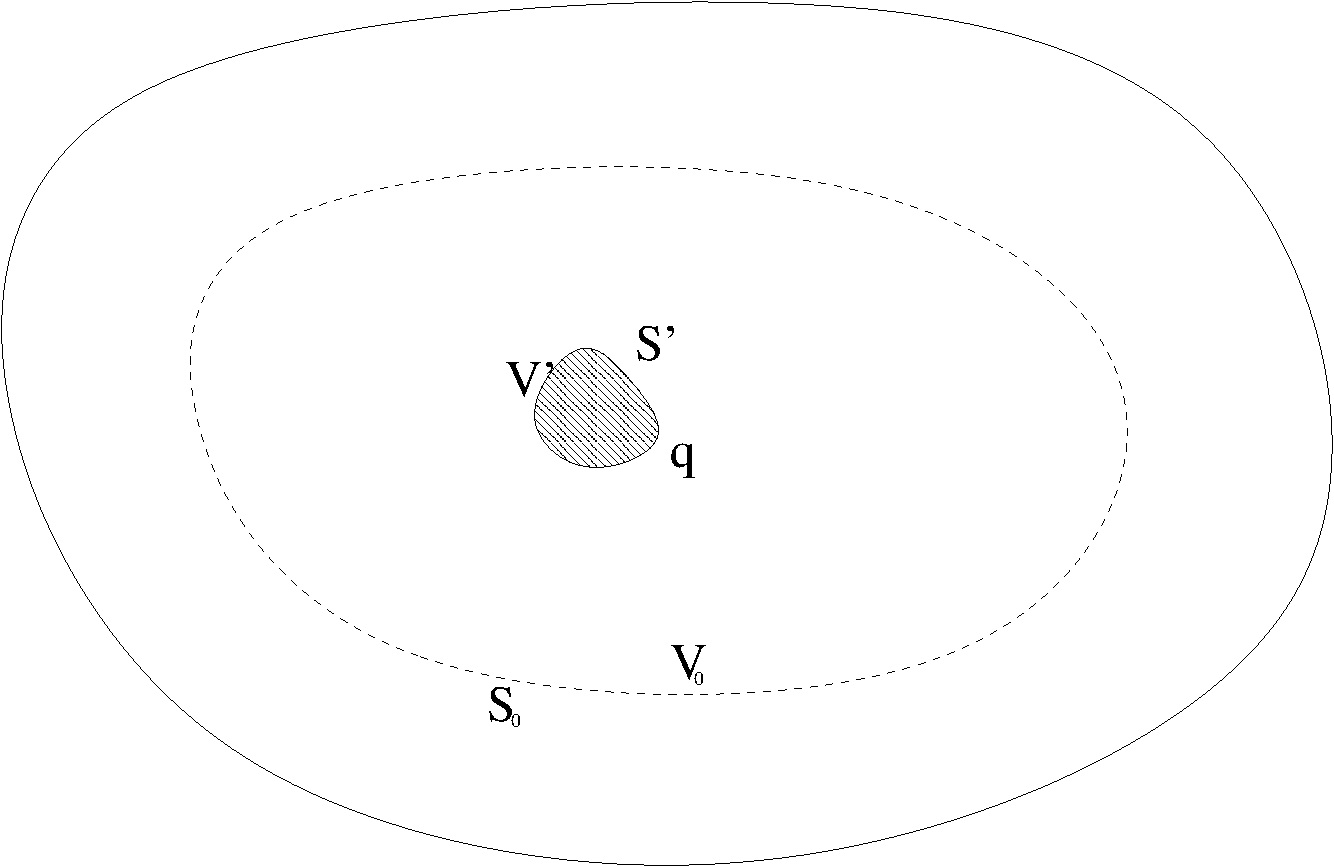
\includegraphics[scale=0.35]{immagini/fisica2/gauss_dielettrici}
\end{figure}
Consideriamo a proposito un dielettrico all'interno del quale sia posta una carica libera $q$ su un conduttore di volume $V'$ e superficie $S'$. Consideriamo una superficie immaginaria $S_0$ racchiudente un volume $V_0$ di dielettrico e il conduttore. Il teorema di Gauss \eqref{teo_Gauss_d1}, quanto quello della circuitazione nel paragrafo precedente, deve valere anche ora considerando tutto le cariche, consideriamo cioè il dielettrico e la carica di polarizzazione come tante cariche nel vuoto:
\begin{equation}
\int_{S_0}\ve E\cdot\ve n\,\ud a=\frac{1}{\varepsilon_0}\left(q+q_p\right)
\label{gauss_dielettrici_3}
\end{equation}
con $q_p$ le cariche di polarizzazione. Vogliamo passare in forma differenziale. D'istinto diremmo $\diver\ve E=\frac{1}{\varepsilon_0}(\rho+\rho_p)$. Ma le $\sigma_p$ che fine fanno? Le cariche di polarizzazione $q_p$ sono:
\begin{equation}
\begin{aligned}
q_p=&\int_{S'}\sigma_p\,\ud a+\int_{V_0-V'}\rho_p\,\ud v=\int_{S'}\ve P\cdot\ve n\,\ud a+\int_{V_0-V'}\!\!\!\!\!-\diver\ve P\,\ud v\\
=&\int_{S'}\ve P\cdot\ve n\,\ud a-\int_{S_0+S'}\ve P\cdot\ve n\,\ud a=-\int_{S_0}\ve P\cdot\ve n\,\ud a
\end{aligned}
\label{qp04}
\end{equation}
Nel primo passaggio abbiamo usato $\rho_p=-\diver\ve P$ e $\sigma_p=\ve P\cdot\ve n$, nel secondo il teorema della divergenza. Nel calcolo non abbiamo considerato la superficie $S_0$ perché non è una superficie fisica del dielettrico\footnote{La questione è delicata. Il risultato della sezione \ref{section:Campo_elettrico_generato_da_un_dielettrico} è valido sia che il volume (la superficie) considerato sia quello del dielettrico o sia un volume (superficie) immaginaria interna al dielettrico. Quindi non è chiaro perché nell'equazione \eqref{qp04} non venga considerato l'integrale su $S_0$. Possiamo fare questo ragionamento: considerando il volume $V_0$ e usando il ragionamento del paragrafo \ref{section:Campo_elettrico_generato_da_un_dielettrico} troviamo una densità di carica superficiale su $S_0$, ma questa non è l'unica carica presente su questa superficie, infatti se consideriamo il volume dato dal volume totale del dielettrico meno $V$ allora troveremo che sulla superficie $S_0$ c'è un'altra carica superficiale che annulla quella precedente. Quindi in generale sulle superfici immaginarie interne ai dielettrici non ci sono cariche superficiali di polarizzazione.}. È come se ci fossero della cariche sulla superficie (immaginaria) $S_0$\footnote{Questo non è in contraddizione con la nota precedente. Infatti se rifacessimo il conto dell'equazione \eqref{qp04} considerando anche la superficie $S_0$ e le cariche indotte su di esso allora sarebbe $q_p=0$, ma poiché non le abbiamo considerate il risultato è proprio quello che manca col segno invertito, cioè $-\int_{S_0}\ve P\cdot\ver n\,\ud  a$. Inoltre possiamo fare quel'altro ragionamento. Consideriamo il dielettrico come formato da due dielettrici separati dalla superficie $S_0$. Il dielettrico interno avrà una carica totale nulla. Quello esterno avrà una carica di polarizzazione sulla superifice $S_0$ con una normale uscente se consideriamo il dielettrico esterno, ma entrante se consideriamo il dielettrico interno. Esso $S_0$ una superficie in comune questa carica superficiale risulta come carica di polarizzazione per il volume immaginario $V_0$.}. Sostituendo la carica di polarizzazione nel teorema di gauss:
\begin{equation}
\varepsilon_0\oint_{S_0}\ve E\cdot\ve n\,\ud a=q-\oint_{S_0}\ve P\cdot\ve n\,\ud a
\end{equation}
usando il teorema della divergenza:
\begin{equation}
\varepsilon_0\int_{V_0}\diver\ve E\,\ud v=\int_{V_0}\rho\,\ud v-\int_{V_0}\diver\ve P\,\ud v=\int_{V_0}(\rho+\rho_p)\,\ud v
\end{equation}
quindi:
\begin{equation}
\diver\ve E=\frac{1}{\varepsilon_0}\left(\rho+\rho_p\right)
\end{equation}
e siamo praticamente tornati al teorema di Gauss per i dielettrici \eqref{gauss_dielettrici_3}.
\subsubsection{Vettore induzione elettrica}
Se sostituiamo l'espressione di $q_p$ data dalla \eqref{qp04} nel teorema di Gauss informa integrale per i dielettrici \eqref{gauss_dielettrici_3} si ottiene:
\begin{equation}
\int_{S_0}\left(\varepsilon_0\ve E+\ve P\right)\cdot n\,\ud a= q
\label{gauss_dielettrici_4}
\end{equation}
Stiamo ottenendo un teorema di gauss che tiene conto solo delle cariche libere $q$. Introduciamo un nuovo vettore:
\begin{Def}[vettore induzione elettrica\index{vettore!induzione!elettrica}]
\begin{equation}
\ve D=\varepsilon_0\ve E+\ve P
\label{vettore_induzione_elettrica01}
\end{equation}
\end{Def}
chiamato anche vettore spostamento elettrico\index{vettore!spostamento!elettrico}. Per l'equazione \eqref{gauss_dielettrici_4} il suo flusso è 
\begin{equation}
\Phi\left(\ve D\right)=q
\end{equation}
con $q$ cariche libere. In forma differenziale, usando il teorema della divergenza, diventa:
\begin{equation}
\diver\ve D=\rho
\end{equation}
con $\rho$ densità di volumetrica di cariche libere.
\[
[D]=\coulomb\per\meter^2
\]
Si sottolinea che il campo elettrico $\ve E$ che compare è il campo elettrico totale, cioè quello creato dalle cariche libere più quelle di polarizzazione.
\section{Suscettività e permittività}
Per chiudere il problema, cioè determinare il campo elettrico serve una nuova equazione, in quanto il campo elettrico è funzione delle cariche di polarizzazione, le quali sono funzione del vettore polarizzazione elettrica il quale è funzione del campo elettrico. Leghiamo direttamente il vettore polarizzazione elettrica con il campo totale:
\begin{equation}
\ve P(\ve r)=\chi_e\ve E(\ve r)
\end{equation}
Dove $\chi_e$ è la suscettività del dielettrico\index{suscettività dielettrica}.
\[
[\chi_e] = \si{}{\farad\per\meter}
\]
Per dielettrici anisotropi è un tensore del second'ordine e quindi $\ve P$ e $\ve E$ non hanno la stessa direzione. Per dielettrici non lineari (quasi sempre con alti campi elettrici) è una funzione di $\ve E$. Per dielettrici omogenei è uno scalare, per i disomogenei una funzione del punto. $\chi_e$ è sempre maggiore di zero, nel vuoto è nullo.

Se sostituiamo nel vettore induzione elettrica \eqref{vettore_induzione_elettrica01} l'ultima espressione introdotta:
\begin{equation}
\ve D=\varepsilon_0\ve E+\chi_e\ve E=\left(\varepsilon_0+\chi_e\right)\ve E
\label{induzione_elettrica16}
\end{equation}
\begin{Def}[costante dielettrica\index{costante!dielettrica}]
\begin{equation}
\varepsilon=\left(\varepsilon_0+\chi_e\right)
\end{equation}
\end{Def}
chiamata anche permittività dielettrica\index{permittività elettrica}
usando questa definizione la \eqref{induzione_elettrica16} diventa:
\begin{equation}
\ve D=\varepsilon\ve E
\end{equation}
\begin{Def}[costante dielettrica relativa]
\begin{equation}
\varepsilon_r=\frac{\varepsilon}{\varepsilon_0}=\left(1+\frac{\chi_e}{\varepsilon_0}\right)
\end{equation}
\end{Def}
chiamata anche permittività dielettrica relativa del mezzo rispetto al vuoto. \`E uno scalare adimensionale e per il vuoto $\varepsilon_r=1$, per i dielettrici è maggiore di $1$. Si ha allora:
\begin{equation}
\varepsilon=\varepsilon_0\varepsilon_r
\end{equation}
\begin{equation}
\ve D=\varepsilon\ve E=\varepsilon_0\varepsilon_r\ve E=\frac{\varepsilon}{\chi_e}\ve P
\end{equation}
Se il mezzo è isotropo i tre vettori $\ve D$, $\ve E$, $\ve P$ sono paralleli.

La relazione che lega $\ve P$ a $\ve E$ oppure equivalentemente $\ve D$ a $\ve E$ è la relazione costitutiva dei materiali per quanto riguarda il comportamento dielettrico.

Per ricordarsi i legami tra $\chi_e$ e $\varepsilon_r$ è utile notare che:
\begin{eqimp}{equation}
 \varepsilon_0 + \chi_e = \varepsilon_0\varepsilon_r
\end{eqimp}
\subsubsection{Altre convenzioni}
In passato $\chi_e$ era definito come
\begin{equation}
\chi_e^\star=\frac{\chi_e}{\varepsilon_0}
\end{equation}
che è adimensionale, quindi le equazioni erano scritte come:
\[
\ve P=\varepsilon_0\chi_e^\star\ve E\qquad\varepsilon=\varepsilon_0\left(1+\chi_e^\star\right)\qquad\varepsilon_r=1+\chi_e^\star\]
\section{Maxwell per i dielettrici}
Nel caso statico siamo in grado di scrivere le equazioni che descrivono totalmente il campo elettrico. Innanzitutto dobbiamo includere la relazione costituiva:
\begin{equation}
\ve D=\ten\varepsilon\ve E
\label{numero_eq01}
\end{equation}
In forma integrale sono:
\begin{gather}
\int_S\ve D\cdot\ve n\,\ud a=Q\\
\oint_C\ve E\cdot\ud\ve l=0
\end{gather}
In forma differenziale:
\begin{gather}
\label{numero_eq03}
\ve\nabla\cdot\ve D=\rho\\
\label{numero_eq02}
\ve\nabla\times\ve E=0
\end{gather}
Le equazioni sono 7 (tre dalla \eqref{numero_eq01}, tre dalla \eqref{numero_eq02}, una dalla \eqref{numero_eq03}), le incognite 7($\rho$,$\ve E$,$\ve D$).
\begin{Es}[carica puntiforme]
 Consideriamo una carica puntiforme $q$ in un dielettrico infinatemente esteso, omogeneo, isotropo e isotropo. Vogliamo calcolare il campo elettrico. Dal teorema di Gauss per i dielettrici $\int_s\ve D\cdot\ver n\,\ud a=q$ si ha che:
 \[
  \ve D = \frac{q}{4\pi}\frac{\ve r}{r^3}
 \]
 quindi da $\ve D=\varepsilon\ve E$ dove $\varepsilon=\varepsilon_0\varepsilon_r$:
 \[
  \ve E = \frac{q}{\giorgi\varepsilon_r}\frac{\ve r}{r^3}
 \]
 come si vede il campo è minore a causa del dielettrico che si è polarizzato. È interessante notare che questo campo elettrico è uguale al campo elettrico nel vuoto di una carica elettrica ridotta pari a $\frac{q}{\varepsilon_r}$. Questo effetto è dato dalla polarizzazione del dielettrico che induce delle cariche di polarizzazione che schermano la carica libera. Calcoliamole; ci serve il vettore di polarizzazione:
 \[
  \ve P(\ve r)=\chi_e\ve E(\ve r) = \frac{q\chi_e}{\giorgi}\frac{\ve r}{r^3}=\frac{q(\varepsilon_r-1)}{4\pi\varepsilon_r}\frac{\ve r}{r^3}
 \]
 spesso si preferisce lavorare in termini di $\varepsilon_r$ piuttosto che di $\chi_e$. Nonostante la polarizzazione non sia uniforme le cariche di polarizzazione volumetriche sono nulle in quanto $\diver \frac{\ve r}{r^3}=0$. Le densità di cariche di polarizzazione saranno sulla superficie del dielettrico. Una superficie è all'infinito, ma non è l'unica infatti anche la carica puntiforme costituisce una superficie. Consideriamo al posto di una carica puntiforme una sfera di raggio $a$. Su questa superficie:
 \[
  \sigma_p = -\frac{q(\varepsilon_r-1)}{4\pi\varepsilon_r}\frac{1}{a^2}
 \]
 avendo usato $\ve r\cdot\ve n=-r$. La carica totale di polarizzazione sulla sfera è
 \[
  q_p = -q\frac{\varepsilon_r-1}{\varepsilon_r}
 \]
 quindi le sorgenti del campo elettrico saranno tutte le cariche, sia quelle libere che quelle di polarizzazione:
 \[
  q + q_p = \frac{q}{\varepsilon_r}
 \]
 e allora abbiamo dimostrato che è come se ci fosse una carica ridotta di un fattore $\varepsilon_r$ nel vuoto.
 
 Il dielettrico complessivamente rimane neutro grazie alle cariche di polarizzazione all'infinito.
\end{Es}

\section{Condizioni al contorno per \texorpdfstring{$\vec E$}{E} e \texorpdfstring{$\vec D$}{D}}
\subsection{\texorpdfstring{$\vec D$}{D} ortogonale}
\begin{figure}[htbp]
\centering
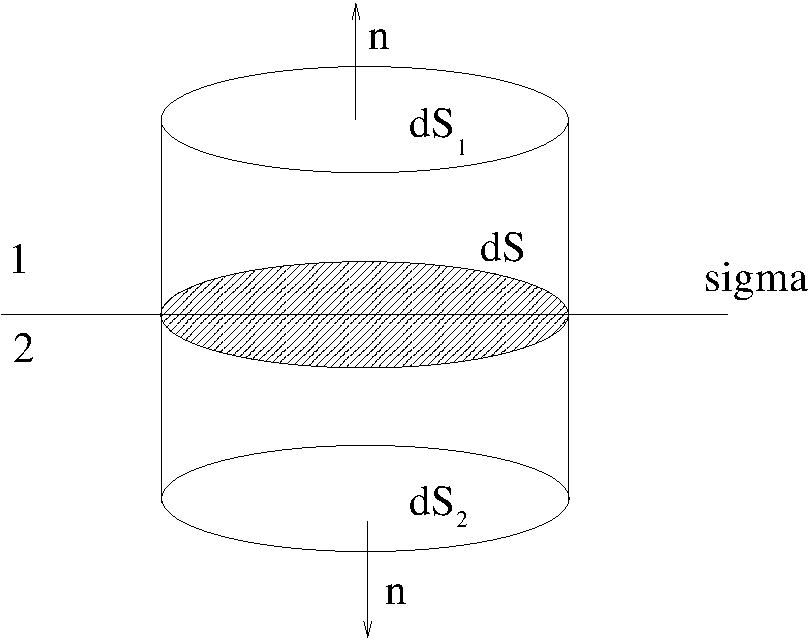
\includegraphics[scale=0.5]{immagini/fisica2/contornoEB}
\end{figure}
Vogliamo sapere cosa succede ai vettori $\ve E$ e $\ve D$ quando si passa da un mezzo ad un altro, sia dielettrico che conduttore. Ipotizziamo che sulla superficie separatrice ci possa essere una distribuzione di carica libera $\sigma(\ve r)$. Consideriamo due mezzi omogenei, lineari, isotropi. La superficie di separazione può essere di qualsiasi forma. Prendiamo un cilindro infinitesimo di basi nei due mezzi aventi area $\ud A$ e altezza $\ud h$ con asse perpendicolare alla superficie di separazione; la superficie di separazione intercettata dal questo risulta piana. Sappiamo che il flusso attraverso tutta la superficie del cilindro:
\begin{equation}
\int_S\ve D\cdot\ve n\,\ud a=\sigma\ud S
\end{equation}
Questa può essere scomposta:
\begin{equation}
\int_{\ud S_1}\ve D_1\cdot\ve n\,\ud a+\int_{\ud S_2}\ve D_2\cdot\ve n\,\ud a+\int_{\ud S_l}\ve D\cdot\ve n\,\ud a=\sigma\ud S
\end{equation}
dove $\ud S_1$ e $\ud S_2$ sono le superfici di base del cilindro, $\ud S_l$ è la superficie laterale. Se facciamo tendere $\ud  h\to 0$ allora l'ultimo integrale si annulla\footnote{può sorgere un problema: come fa $\ud h\to 0$ se il cilindro è già infinitesimo? Bisogna considerare la superficie laterale di ordine d'infinitesimo maggiore dell'ordine di infinitesimo dell'area delle basi}. Facciamo già il prodotto scalare: $\ve D_1\cdot \ve n=D_{1n}$, $\ve D_2\cdot \ve n=-D_{2n}$; queste due componenti sono nella direzione ortogonale alla superficie di separazione e il verso positivo è quello di $n$ nel primo mezzo (in figura verso l'alto):
\begin{equation}
\int_{\ud S_1} D_{1n}\,\ud a-\int_{\ud S_2}D_{2n}\,\ud a=\sigma\ud A
\end{equation}
$\ud S_1$, $\ud S_2$ sono infinitesimi, quindi $D_{1n}$ e $D_{2n}$ sono\footnote{usare $\ve D_1$ e $\ve D_2$ serve solo per distinguere dove è calcolato $\ve D$, ma è sempre e solo $\ve D$ che stiamo calcolando} uniformi sulle superfici, possiamo svolgere l'integrale:
\begin{equation}
D_{1n}\ud A_1-D_{2n}\ud A_2=\sigma\ud A
\end{equation}
\begin{equation}
D_{1n}-D_{2n}=\sigma
\label{D_normale02}
\end{equation}
Se non c'è carica sulla superficie di separazione allora le due componenti normali sono uguali e $D_n$ varia con continuità. In generale se ogni volta che usciamo da una superficie (cioè ci muoviamo nella direzione della sua normale) la componente normale uscente di $D$ aumenta.
\subsection{\texorpdfstring{$\vec E$}{E} tangente}
\begin{figure}[htbp]
\centering
\begin{tikzpicture}[scale=4]
\draw[style=dashed] (-1,0) node[above right] {$1$} node[below right] {$2$} -- (1,0);
\draw (-.8,-.4) -- (-.8,.4) node[below right]{$C$};
\draw (.8,.4) -- (.8,-.4);
\draw (-.8,-.4) -- (0,-.4);
\draw[<-] (0,-.4) node[below] {$\ud\ve l_1$} -- (.8,-.4);
\draw[->] (-.8,.4) -- (0,.4) node[above] {$\ud\ve l_2$};
\draw (0,.4) -- (.8,.4);
\end{tikzpicture}%

\end{figure}
Calcoliamo la circuitazione su $C$, un rettangolo con lati $\ud l_1$ e $\ud l_2$ paralleli alla superficie di separazione, altezze $\ud h_1$ e $\ud h_2$, in modo tale che la sua superficie contenga la separazione tra i due mezzi. Il rettangolo è infinitesimo e quindi la superficie di separazione di qualsiasi forma è vista da $C$ come un piano. Sappiamo che la circuitazione di $\ve E$ deve essere nulla, o equivalentemente che il rotore di $\ve E$ è zero:
\begin{equation}
\oint_C\ve E\cdot \ud l=0
\end{equation}
Lo spezziamo:
\begin{equation}
\int_{\ud l_1}\ve E_1\cdot\ud\ve l_1+\int_{\ud l_2}\ve E\cdot\ud\ve l_2+\int_{\ud h_1}\ve E\cdot\ud\ve l+\int_{\ud h_2}\ve E\cdot\ud\ve l
\end{equation}
facciamo\footnote{ancora: $\ud h$ deve essere di ordine di infinitesimo maggiore di $\ud l$} $\ud h\to 0$ e il prodotto scalare considerando che $\ud\ve l_1=-\ud\ve l_2$:
\begin{equation}
\int_{\ud l_1}E_{1\tan}\ud l_1-\int_{\ud l_2}E_{2\tan}\ud l_2=0
\end{equation}
Essendo $\ud l_1$, $\ud l_2$ infinitesimi $\ve E$ si mantiene costante su di essi e possiamo svolgere l'integrale:
\begin{equation}
\ve E_{1\tan}=\ve E_{2\tan}
\end{equation}
essendo $\ud l_1=\ud l_2$. La componente tangente varia con continuità.

Riprendiamo l'equazione sulla componente normale di $\ve D$ \eqref{D_normale02} nell'ipotesi che sulla superficie non ci sia carica libera:
\begin{equation}
D_{1n}=D_{2n}
\end{equation}
cioè la componente di $\ve D$ normale alla superficie di separazione varia con continuità. Usando:
\begin{equation}
\ve D=\varepsilon\ve E=\varepsilon_0\varepsilon_r \ve E
\end{equation}
\begin{equation}
\varepsilon_0\varepsilon_{r1} E_{1n}=\varepsilon_0\varepsilon_{r2} E_{2n}
\end{equation}
quindi la componente normale di $\ve E$ non varia con continuità.
\begin{equation}
\frac{E_{1n}}{E_{2n}}=\frac{\varepsilon_{r2}}{\varepsilon_{r1}}
\end{equation}
In modo analogo si può mostrare che anche la componente di $\ve D$ tangente subisce discontinuità.
\begin{equation}
\frac{D_{1\tan}}{D_{2\tan}}=\frac{\varepsilon_{r2}}{\varepsilon_{r1}}
\end{equation}
\begin{Es}[piano di separazione]
 Riproponiamo l'esempio \ref{es:carica_e_piano_infinito} a pagina \pageref{es:carica_e_piano_infinito} ma al posto del conduttore mettiamo un dielettrico. In particolare consideriamo due dielettrici caratterizzate da $\varepsilon_1$ e $\varepsilon_2$ separati da un piano $z=0$ e una carica puntiforme nel primo dielettrico, distante $d$ dal piano. Le equazioni differenziali del problema sono:
 \begin{gather*}
  \ve\nabla\cdot\ve D = \varepsilon_0\varepsilon_r(z)\ve\nabla\cdot\ve E = \rho \\
  \ve\nabla\times\ve E = 0
 \end{gather*}
 dove $\varepsilon_r(z)$ è uguale a $\varepsilon_1$ per $z$ positivi e $\varepsilon_2$ altrimenti. Le condizioni al bordo sono:
 \begin{gather*}
  \varepsilon_0\varepsilon_2 E_z(x,y,0^-) = D_z(x,y,0^-) = D_z(x,y,0^+) = \varepsilon_0\varepsilon_1 E_z(x,y,0^+) \\
  E_x(x,y,0-) = E_x(x,y,0+) \\
  E_y(x,y,0-) = E_y(x,y,0+)
 \end{gather*}
 cioè abbiamo imposto la continuità sulla componente normale di $\ve D$ (non essendoci cariche libere sulla superficie di separazione) e la continuità sulle componenti tangenti di $\ve E$. Risolviamo il problema per la regione dove è presente la carica puntiforme. Per simulare le condizioni al bordo aggiungiamo una carica immagine puntiforme all'esterno della regione in considerazione. Per ragioni di simmetria la carica immagine sarà in posizione simmetrica rispetto alla carica reale. Poiché $\rot\ve E =0$ possiamo sempre considerare un potenziale. Considerando le due cariche:
 \[
  \varphi(\ve r) = \frac{1}{\giorgi\varepsilon_1}\left(\frac{q}{\norm{\ve r-\ve r_q}}+\frac{q'}{\norm{\ve r-\ve r_q'}}\right)
 \]
 questa è la soluzione per $z>0$. Nell'altro semispazio non ci sono cariche; l'unica carica che consideriamo è una carica immagine per simulare le condizioni al contorno. Questa carica sarà all'esterno della regione, quindi sarà in $z>0$ e scegliamo che sia nella posizione della carica vera:
 \[
  \varphi(\ve r) = \frac{1}{\giorgi\varepsilon_2}\frac{q''}{\norm{\ve r-\ve r_q''}}
 \]
 Per trovare $q'$ e $q''$ basta imporre le condizioni al contorno. Calcoliamo $E_z(x,y,0^\pm)$:
 \begin{equation*}
 \begin{aligned}
  E_z(x,y,0^-) &= -\frac{\partial}{\partial z}\varphi(x,y,0^-) = \frac{q''}{\giorgi\varepsilon_2}\left(\frac{(z-z_q'')}{\norm{\ve r-\ve r_q''}^3}\right)_{z=0}\\
  &=\frac{q''}{\giorgi\varepsilon_2}\left(\frac{-d}{\left(x^2+y^2+d^2\right)^{3/2}}\right)
  =-\frac{q''}{\giorgi\varepsilon_2}\left(\frac{d}{\left(\rho^2+d^2\right)^{3/2}}\right)\\
  E_z(x,y,0^+) &= -\frac{\partial}{\partial z}\varphi(x,y,0^+) = \frac{1}{\giorgi\varepsilon_1}\left(q\frac{(z-z_q)}{\norm{\ve r-\ve r_q}^3}+q'\frac{(z-z_q')}{\norm{\ve r-\ve r_q'}^3}\right)_{z=0}\\
  &=\frac{q'-q}{\giorgi\varepsilon_1}\left(\frac{d}{\left(\rho^2+d^2\right)^{3/2}}\right)  
 \end{aligned} 
 \end{equation*}
 ricordando che $z_q=z_q''=-z_q' = d$, $x_q=x_q'=x_q''=y_q=y_q'=y_q''=0$ e $\rho = \sqrt{x^2+y^2}$. Uguagliano $\varepsilon_2E_z(x,y,0^-)=\varepsilon_1E_z(x,y,0^+)$ si ottiene:
 \[
  q''=q-q'
 \]
 Per le componenti tangenziali calcoliamo la componente $x$:
 \begin{equation*}
 \begin{aligned}
  E_x(x,y,0-) &= -\frac{\partial}{\partial x}\varphi(x,y,0^-) = \frac{q''}{\giorgi\varepsilon_2}\frac{x}{(\rho^2+d^2)^{3/2}}\\
  E_x(x,y,0+) &= -\frac{\partial}{\partial x}\varphi(x,y,0^+) = \frac{1}{\giorgi\varepsilon_1}\left(\frac{qx}{(\rho^2+d^2)^{3/2}}+\frac{q'x}{(\rho^2+d^2)^{3/2}}\right)
 \end{aligned}
 \end{equation*}
 uguagliandole:
 \[
  \frac{q''}{\varepsilon_2}=\frac{q+q'}{\varepsilon_1}
 \]
 usando la componente $y$ non si ottiene nulla in più, infatti il problema ha simmetria cilindrica e quindi è simmetrico rispetto allo scambio $x\leftrightarrow y$\footnote{Questo non vuol dire che la componente $y$ è inutile. Infatti abbiamo usato la simmetria per decidere che le cariche immagini sono sull'asse $z$. Se non l'avessimo fatto allora avremmo avuto bisogno anche di questa equazione.}. Usando le due equazioni trovate, risolvendo il sistema:
 \[
  q' = \frac{\varepsilon_1-\varepsilon_2}{\varepsilon_1+\varepsilon_2}q\qquad q'' = \frac{2\varepsilon_2}{\varepsilon_1+\varepsilon_2}q
 \]

 Per calcolare la carica di polarizzazione serve il vettore di polarizzazione: $\ve P = \chi_e\ve E=\varepsilon_0(\varepsilon_r-1)\ve E$. La divergenza di $\ve P$ è nulla in quanto dal teorema di Gauss la divergenza di $\ve E$ è nulla, tranne che nelle cariche puntiformi. Quindi la densità volumetriche di polarizzazione sono nulle. Le cariche superficiali sono invece sulla superficie di separazione:
 \[
  \sigma_\text{pol} = \ve P_1\cdot\ve n+\ve P_2\cdot\ve n = -\varepsilon_0(\varepsilon_1-1)\ve E_z(x,y,0^+)-\varepsilon_0(\varepsilon_2-1)\ve E_z(x,y,0^-)
 \]
 Il campo elettrico sul piano l'abbiamo già calcolato, quindi sostituendo, dopo varie semplificazioni:
 \[
  \sigma_\text{pol} = \frac{1}{2\pi}\frac{\varepsilon_1-\varepsilon_2}{\varepsilon_1(\varepsilon_1+\varepsilon_2)}\frac{d}{(\rho^2+d^2)^{3/2}}
 \]
 Riassumiamo con dei grafici quanto trovato. In figura \ref{fig:campo_piano_dielettrico} è rappresentato il potenziale elettrico, con le linee di forza del campo elettrico.
 \begin{figure}[htbp]
  \centering
  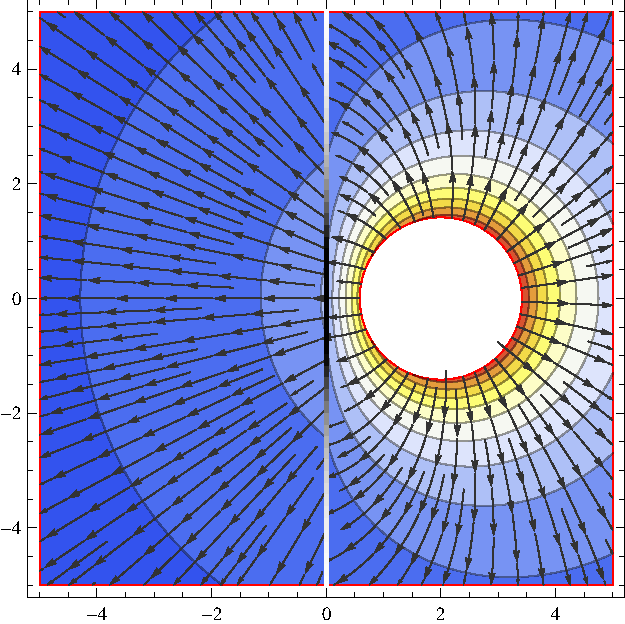
\includegraphics{immagini/fisica2/campo_due_dielettrici1}
  \caption{Potenziale e campo elettrico per una carica con due regioni con costante dielettrica diversa. In particolare $\varepsilon_2 \text{(sinistra)}>\varepsilon_1\text{(destra).}$. Il colore del piano è proporzionale alla carica di polarizzazione. Il bordo rosso indica il limite della regione del grafico.}
  \label{fig:campo_piano_dielettrico}
 \end{figure}
 \begin{figure}[htbp]
  \centering
  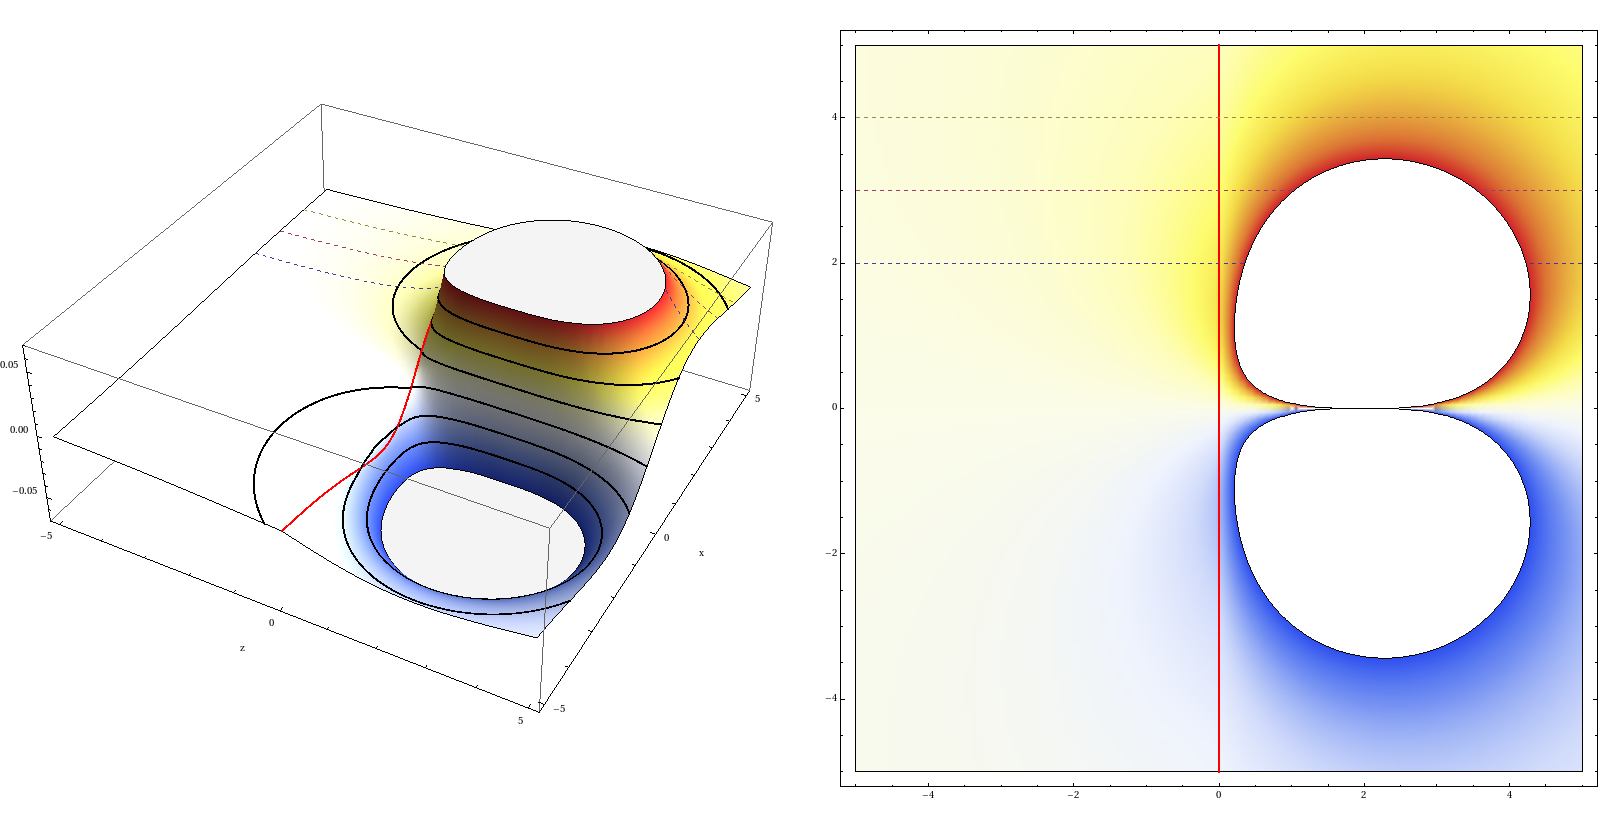
\includegraphics[scale=0.2]{immagini/fisica2/campo_due_dielettrici2}
  \caption{Componente parallela al piano del campo elettrico. Come si nota non ci sono discontinuità. La linea rossa è il piano.}
  \label{fig:campo_piano_dielettrico2}
 \end{figure}
 
 \begin{figure}[htbp]
  \centering
  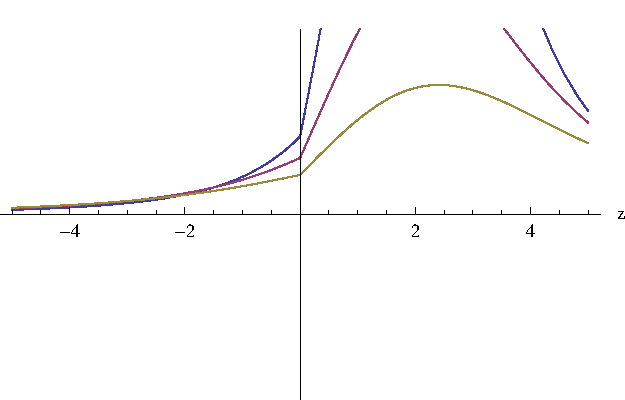
\includegraphics{immagini/fisica2/campo_due_dielettrici4}
  \caption{Componente parallela al piano del campo elettrico lungo le linee orizzontali della figura precedente.}
  \label{fig:campo_piano_dielettrico4}
 \end{figure}
 
 \begin{figure}[htbp]
  \centering
  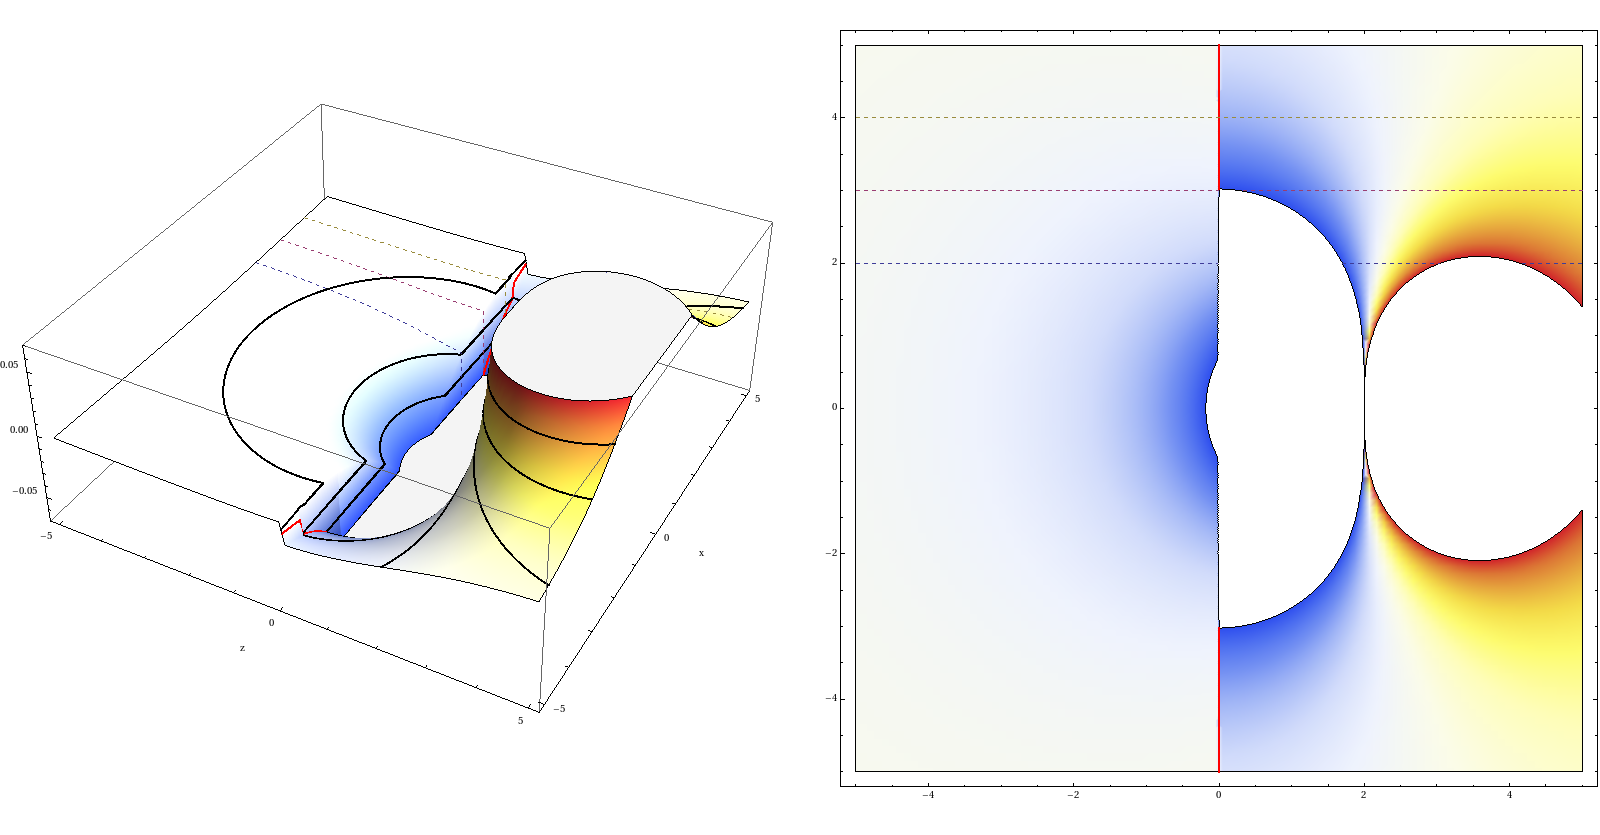
\includegraphics[scale=0.2]{immagini/fisica2/campo_due_dielettrici3}
  \caption{Componente normale al piano del campo elettrico. Come si nota c'è una discontinuità. La linea rossa è il piano.}
  \label{fig:campo_piano_dielettrico3}
 \end{figure}
 
 \begin{figure}[htbp]
  \centering
  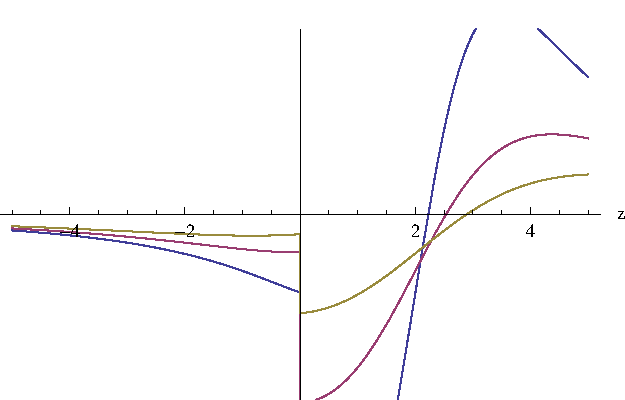
\includegraphics{immagini/fisica2/campo_due_dielettrici5}
  \caption{Componente normale al piano del campo elettrico lungo le linee orizzontali della figura precedente.}
  \label{fig:campo_piano_dielettrico5}
 \end{figure}
 
 Si noti che questo esempio è un caso generale dell'esempio \ref{es:carica_e_piano_infinito} in cui al posto dei dielettrici c'era il vuoto e un piano conduttore. L'esempio particolare si ottiene con $\varepsilon_1=1$ e $\varepsilon_2=\infty$. Infatti in questo caso: $q'=-q$ e $q''=0$. 
\end{Es}

\begin{Es}[Sfera dielettrico polarizzata]
 Immaginiamo un dielettrico sferico uniformemente polarizzato con il vettore di polarizzazione $\ve P$ rivolto come l'asse $z$. Il potenziale da esso generato sarà:
 \[
  \varphi = \frac{1}{\giorgi}\int_{\text{sfera}} \frac{\ve P\cdot (\ve r-\ve r')}{\norm{\ve r-\ve r'}^3}
 \]
 questo conto è complicato e quindi cerchiamo un trucco. Si tratta di schematizzare la sfera polarizzata come un dipolo. Per ragioni di simmetria le due cariche del dipolo giacciono sull'asse $z$. Si può immaginare che l'effetto della polarizzazione sia di separare le cariche positive e negative di $\delta$ nella direzione di $\ve P$. Il nostro sistema allora è equivalente a un sistema di due sfere cariche uniformemente con segno opposto e separate di $\delta$. A grande distanza le due sfere diventano due punti di carica $\pm Q$ e quindi il momento di dipolo $\ve p=Q\delta$ e il vettore di polarizzazioen $\ve P=\rho\delta$.
 
 Il campo generato all'interno della sfera sarà quello della somma dei campi generati dalle due sfere. Il campo generato da una sfera carica uniformente si può trovare con il teorema di gauss:
 \[
  4\pi r^2 E = \frac{4}{3}\pi r^3\rho
 \]
 cioè:
 \[
  E_{\pm}(\ve r) = \frac{\rho}{3\varepsilon_0}\ve r
 \]
 se $\ve r_+$ e $\ve r_-$ sono le distanze dei centri delle sfere da un punto generico allora in questo punto il campo totale sarà:
 \[
  E(\ve r) = \frac{\rho}{3\varepsilon_0}(\ve r-\ve r')
 \]
 ma $(\ve r-\ve r') = -\delta$ quindi all'interno della sfera polarizzata:
 \[
  \ve E = -\frac{\rho}{3\varepsilon_0}\ve\delta=-\frac{P}{3\varepsilon_0}
 \]
 
 All'esterno invece usiamo l'appossimazione di dipolo con momento di dipolo $\ve p=\frac{4}{3}\pi R^3\rho\ve\delta=\frac{4}{3}\pi R^3\ve P$. Poichè $\ve P$ è diretto lungo l'asse $z$ usando l'espressione \eqref{eq:E_dipolo}:
 \[
  \ve E(\ve r) = \frac{1}{\giorgi}\left\{3(\ve p\cdot\ve r)\frac{\ve r}{r^5}-\frac{\ve p}{r^3}\right\} = \frac{R^3}{\varepsilon_0}\left\{Pz \frac{\ve r}{r^5}-\frac{\ve P}{3r^3}\right\}
 \]
 
 La carica di polarizzazione sarà
 \[
  \sigma_p = \ve P\cdot \ver n = P\cos\theta
 \]


\end{Es}


\section{Energia del campo elettrostatico}
Consideriamo $N$ conduttori con superfici $S_i, i=1\ldots N$. Partiamo dall'equazione \eqref{energia_sistema_cariche} che descrive l'energia per un sistema di cariche puntiformi:
\begin{equation}
\label{eq:en_cariche_puntiformi}
W=\frac{1}{2}\sum_{i=1}^n\sum_{i\neq j}^n\frac{q_iq_j}{4\pi\varepsilon_0}\frac{1}{\norm{r_i-r_j}}=\frac{1}{2}\sum_{i=1}^{N}q_i\varphi
\end{equation}
Nel nostro caso le cariche sono date dalle distribuzioni $\sigma(\ve r)$ sulle superfici e $\rho(\ve r)$ all'esterno dei conduttori (nei conduttori la carica si distribuisce solo sulla superficie). Sia $S=\bigcup_{i=1}^n S_i$ e $V$ il volume esterno ai conduttori:
\begin{equation}
\begin{split}
W&=\frac{1}{2}\int_V\varphi\rho\,\ud v+\frac{1}{2}\int_S\varphi\sigma\,\ud a=
\frac{1}{2}\int_V\varphi\diver\ve D\,\ud v+\frac{1}{2}\int_S\varphi\sigma\,\ud a\\
&=\frac{1}{2}\int_V\diver(\varphi\ve D)\,\ud v-\frac{1}{2}\int_V\ve D\cdot\grad\varphi\,\ud v+\frac{1}{2}\int_S\varphi\sigma\,\ud a\\
&=\frac{1}{2}\int_V\diver(\varphi\ve D)\,\ud v+\frac{1}{2}\int_V\ve D\cdot\ve E\,\ud v+\frac{1}{2}\int_S\varphi\sigma\,\ud a\\
&=\frac{1}{2}\int_{S_V}\varphi\ve D\cdot\ve n\,\ud a+\frac{1}{2}\int_V\ve D\cdot\ve E\,\ud v+\frac{1}{2}\int_S\varphi\sigma\,\ud a
\end{split}
\end{equation}
dove $S_V$ è la superficie che delimita il volume $V$ (il volume esterno alle superfici $S_i$, in quanto all'interno dei conduttori $\rho=0$). $S_V$ è composta da una superficie limite all'infinito $S_\infty$ e dalle superfici dei conduttori.
\begin{equation}
W=\frac{1}{2}\int_{S_\infty}\varphi\ve D\cdot\ve n\,\ud a+\frac{1}{2}\int_{S}\varphi\ve D\cdot\ve n\,\ud a+\frac{1}{2}\int_V\ve D\cdot\ve E\,\ud v+\frac{1}{2}\int_S\varphi\sigma\,\ud a
\end{equation}
Sappiamo che $\varphi$ varia come $\frac{1}{r}$, $\ve D$ come $\frac{1}{r^2}$ e $\ud a$ come $r^2$, quindi il primo integrando va come $\frac{1}{r}$ e l'integrale si annulla.
\begin{equation}
W=\frac{1}{2}\int_{S}\varphi\ve D\cdot\ve n\,\ud a+\frac{1}{2}\int_V\ve D\cdot\ve E\,\ud v+\frac{1}{2}\int_S\varphi\sigma\,\ud a
\end{equation}
ma $\ve D\cdot\ve n=-\sigma$ in quanto le normali sono dirette verso l'interno delle superfici conduttrici:
\begin{equation}
W=\frac{1}{2}\int_V\ve E\cdot\ve D\,\ud v=\frac{1}{2}\varepsilon\int_V E^2\,\ud v
\end{equation}
e la densità di energia $w$:
\begin{equation}
\label{eq:en_campo_el}
w=\frac{1}{2}\ve E\cdot\ve D=\frac{1}{2}\varepsilon E^2
\end{equation}

\subsection{Self-energy}
Come si nota dalla \eqref{eq:en_campo_el} la densità di energia del campo elettrostatico è definita positiva, quindi anche il suo integrale, cioè l'energia totale è sempre positiva. Questa è una contraddizione con l'equazione \eqref{eq:en_cariche_puntiformi}, per esempio se consideriamo due cariche, una positiva e l'altra negativa:
\[
 W = \frac{1}{\giorgi} \frac{q_1 q_2}{\norm{\ve r_1-\ve r_2}}
\]
Il problema è che l'equazione \eqref{eq:en_campo_el} contiene termini di autointerazione, mentre la \eqref{eq:en_cariche_puntiformi} no. Infatti proviamo a calcolare la densità di energia per il sistema formato dalle due cariche. Il campo elettrostatico:
\[
 \ve E(\ve r) = \frac{1}{\giorgi} \left(\frac{q_1(\ve r-\ve r_1)}{\norm{\ve r-\ve r_1}^3}+\frac{q_2(\ve r-\ve r_2)}{\norm{\ve r-\ve r_2}^3}\right)
\]
e quindi la densità di energia:
\[
 w = \frac{1}{2}\varepsilon_0 E^2 = \frac{\varepsilon_0}{2(\giorgi)^2}\left(\frac{q_1^2}{\norm{\ve r-\ve r_1}^4}+\frac{q_2^2}{\norm{\ve r-\ve r_2}^4}+2\frac{q_1q_2(\ve r-\ve r_1)\cdot(\ve r-\ve r_2)}{\norm{\ve r-\ve r_1}^3\norm{\ve r-\ve r_2}^3}\right)
\]
I primi due termini rappresentano i termini di autointerazione. Tralasciando questi e cosiderando solo il rimanente calcoliamo l'energia totale integrando sul volume:
\[
 W = \frac{q_1q_2}{16\pi^2\varepsilon_0} \int_V \frac{(\ve r-\ve r_1)\cdot(\ve r-\ve r_2)}{\norm{\ve r-\ve r_1}^3\norm{\ve r-\ve r_2}^3}\,\ud v
\]
usiamo la sostituzione $\ve x = \frac{\ve r-\ve r_1}{\norm{\ve r_1-\ve r_2}}$, da cui $\ve r=\norm{\ve r_1-\ve r_2}\ve x+\ve r_1$ e $\ud v=\ud^3 \ve r = \norm{\ve r_1-r_2}^3\,\ud^3\ve x$:
\begin{equation*}
\begin{aligned}
 W &= \frac{q_1q_2}{16\pi^2\varepsilon_0} \int_V \frac{\ve x\norm{\ve r_1-\ve r_2}}{\norm{\ve r_1-\ve r_2}^3\norm{\ve x}^3}\frac{\norm{\ve r_1-\ve r_2}(\ve x+\ve n)}{\norm{\ve r_1-\ve r_2}^3\norm{\ve x+\ve n}^3} \norm{\ve r_1-\ve r_2}^3\,\ud^3\ve x\\
   &= \frac{q_1q_2}{16\pi^2\varepsilon_0}\frac{1}{\norm{\ve r_1-\ve r_2}} \int_V \frac{\ve x\cdot (\ve x+\ve n)}{x^3\norm{\ve x+\ve n}^3}\,\ud^3\ve x
 \end{aligned}
\end{equation*}
con $\ve n=\frac{\ve r_1-\ve r_2}{\norm{\ve r_1-\ve r_2}}$. Occupiamoci dell'integrale, in coordinate polari diventa:
\begin{equation*}
\begin{aligned}
  & 2\pi\int \frac{x^2+x\cos\theta}{x^3(x^2+1+2x\cos\theta)^{3/2}} \sin\theta x^2\,\ud x\ud\theta\\
 =& -2\pi\int\ud x\int_{1}^{-1} \frac{x+y}{(x^2+1+2xy)^{3/2}} \,\ud y\\
 =& 2\pi\int\ud x\left\{ \left[-\frac{1}{x\sqrt{x^2+1+2 xy}}(x+y)\right]_{-1}^1+\int_{-1}^{1}\frac{1}{x\sqrt{x^2+1+2xy}}\,\ud y\right\}\\
 =& 2\pi\int\ud x\left[ -\frac{1}{x\sqrt{x^2+1+2 xy}}(x+y)+\frac{1}{x^2}\sqrt{x^2+1+2x y}\right]_{-1}^1\\
 =& 2\pi\int\ud x\left[\frac{1+xy}{x^2\sqrt{2xy+x^2+1}}\right]_{y=-1}^1\\
\end{aligned}
\end{equation*}
avendo usato l'integrazione per parti e la sostituzione $z=x^2+1+2xy$. Valutando gli estremi:
\begin{equation*}
\begin{aligned}
  & 2\pi\int\ud x\left[\frac{1+x}{x^2\sqrt{2x+x^2+1}}-\frac{1-x}{x^2\sqrt{-2x+x^2+1}}\right]\\
 =& 2\pi\int\ud x\left[\frac{1+x}{x^2|1+x|}-\frac{1-x}{x^2|1-x|}\right]\\
 =& 2\pi\int\ud x\frac{\sgn(x+1)+\sgn(x-1)}{x^2}
\end{aligned}
\end{equation*}
L'integrale è facile perché la somma delle due funzioni segno fa:
\begin{equation*}
\sgn(x+1)+\sgn(x-1)=
 \begin{cases}
  -2 & x<1\\
  +2 & x>1\\
  0  & \text{altrimenti}
 \end{cases}
\end{equation*}
quindi l'integrale in $x$:
\[
   2\pi\int_1^\infty\frac{2}{x^2}\ud x = 2\left[-\frac{1}{x}\right]_1^\infty=4\pi
\]
allora l'energia totale:
\[
 W= \frac{q_1q_2}{16\pi^2\varepsilon_0}\frac{1}{\norm{\ve r_1-\ve r_2}} \int_V \frac{\ve x\cdot (\ve x+\ve n)}{x^3\norm{\ve x+\ve n}^3}\,\ud^3\ve x =  \frac{q_1q_2}{\giorgi}\frac{1}{\norm{\ve r_1-\ve r_2}}
\]
come voluto.



\chapter{Magnetostatica nei mezzi materiali}
\minitoc
\section{Magnetizzazione}
Ogni atomo è assimilabile ad una spira percorsa da corrente che ha un certo momento magnetico, chiamato momento di dipolo orbitale magnetico, per esempio per l'atomo di idrogeno:
\[
\ve m=-\frac{e}{T}S\ve n
\]
dove $S$ è la superficie racchiusa dalla traiettoria dell'elettrone, e $T$ il periodo dell'orbita. Il momento magnetico può essere scritto anche in termini di momento magnetico $\ve L=m_er^2 \omega\ve n$: $\ve m=-\frac{e}{m_e}\ve L$ (vedi \ref{momento_magnetico_orbitale}). A questo va aggiunto il momento magnetico di dipolo intrinseco o di spin dovuto all'elettrone\footnote{in un contesto classico lo spin dell'elettrone può essere immaginato come il momento angolare dovuto ad una rotazione dell'elettrone; in realtà per dimostrare l'esistenza dello spin è necessaria la meccanica quantistica relativistica.}. In realtà anche i protoni e in neutroni contribuiscono al momento magnetico totale $\ve m$. Riconduciamo il fenomeno della magnetizzazione alle correnti atomiche, come aveva intuito Ampere. Possiamo immaginare che il momento di dipolo magnetico sia dovuto alla presenza di cariche magnetiche $q_m$:
\begin{equation}
\ve m=q_m\ve\delta
\end{equation}
\begin{Def}[intensità di magnetizzazione]
\begin{equation}
\ve M=\frac{\sum_i\ve m_i}{\Delta V}
\label{intensita_magnetizzazione}
\end{equation}
usando sempre la convenzione di $\Delta V$ piccolo dal punto di vista macroscopico e grande dal punto di vista microscopico. Il vettore intensità di magnetizzazione è anche detto semplicemente magnetizzazione.
\end{Def}
Se non applichiamo un campo magnetico esterno mediamente $\ve M$ è nullo in quanto $\ve m$ è orientato casualmente nello spazio. Per alcuni materiali questo non è del tutto vero. Quando applichiamo un campo magnetico esterno questo crea una coppia di forze sui dipoli che tende a farli disporre secondo un orientamento, allora $\ve M$ è diverso da zero e il materiale è magnetizzato. Il momento che si crea:
\[
\ve\tau=\ve m\times\ve B
\]
I materiali paramagnetici aumentano il campo magnetico in quanto i dipoli magnetici si orientano come il campo esterno. Nei materiali diamagnetici invece $\ve M$ è opposto a $\ve B$ e quindi il campo magnetico diminuisce.
\subsubsection{unità}
\[
\left[m\right]=\ampere\meter\squared
\qquad
\left[q_m\right]=\ampere\meter
\qquad
\left[M\right]=\ampere\per\meter
\]
\section{Approccio teorico}
Un materiale magnetizzato può essere studiato facendo ricorso alle correnti di magnetizzazione oppure usando i dipoli magnetici. Usando il secondo approccio non si fa altro che rifare quello che è stato fatto per i dielettrici, cioè trovare delle densità di carica fittizie che interpretino i fenomeni. Usando i dipoli si userà il potenziale scalare magnetico, mentre usando le correnti di magnetizzazione il potenziale scalare magnetico.
\begin{center}
$
\xymatrix{
\ve{J_m}&&&&\sigma_m,\rho_m\\
\ar[dd]&\ar[dr]&&\ar[dl]&\ar[dd]\\
&&\ve M&&\\
\ve A&&&&\varphi_m\\
\ar[d]&&&&\ar[d]\\
\ve B=\rot\ve A&&&&\ve B=-\mu_0\grad\varphi_m
}$\end{center}
\section{Correnti di magnetizzazione}
Se consideriamo un materiale magnetico caratterizzato da un vettore magnetizzazione $\ve M\neq 0$ lo possiamo vedere come formato da spire elementari, tutte percorse da una corrente nello stesso verso, dato dal vettore $\ve M$. Se $\ve M$ è uniforme allora si ha che le correnti di spire adiacenti si annullano, quello che rimane sono delle correnti che percorrono la superficie del materiale. La densità di corrente che si genera è massima sulle superfici parallele a $\ve M$ e nulla sulle superfici ortogonali a $\ve M$. Deve essere:
\[
\ve J\propto \ve M\times\ve n
\]

Consideriamo una magnetizzazione non uniforme. In questo caso le correnti elementari adiacenti non si annullano totalmente, la risultante è una corrente macroscopica all'interno del materiale, oltre alla corrente superficiale.

Consideriamo il caso generale di un materiale non uniformemente magnetizzato. Consideriamo due parallelepipedi infinitesimi di volume $\ud V_1$ e $\ud V_2$, di lati $\ud x$, $\ud y$, $\ud z$, adiacenti lungo la direzione $y$. Se nel primo volumetto c'è una magnetizzazione $\ve M(x,y,z)$ nel secondo sarà:
\begin{equation}
\ve M(x,y+\ud y,z)=\ve M+\frac{\partial\ve M}{\partial y}\ud y
\end{equation}
consideriamo la componente $x$. Dalla \eqref{intensita_magnetizzazione} possiamo dire che la componente $x$ del momento magnetico sia:
\begin{equation}
\ud m_x=M_x\ud V=\ud m_x\ud x\ud y\ud z
\end{equation}
ma sappiamo anche che $\ud \ve m=I\ud S\ve n$, quindi nel nostro caso dobbiamo considerare la corrente che si avvolge nel piano perpendicolare a $M_x$:
\begin{equation}
\ud m_x=I_{m1}\ud S=I_{m1}\ud y\ud z
\end{equation}
dove $I_{m1}$ è la corrente di magnetizzazione ortogonale a $M_x$ nel primo volume. Dal confronto delle ultime due equazioni:
\begin{equation}
I_{m1}=M_x\ud x
\end{equation}
Per il secondo volume invece:
\begin{equation}
I_{m2}=\left(M_x+\frac{\partial M_x}{\partial y}\ud y\right)\ud x
\end{equation}
Sommando le due correnti di magnetizzazione (col segno) troviamo la corrente che passa nel tratto verticale in comune:
\begin{equation}
I_{mz}'=I_{m1}-I_{m2}=M_x\ud x-\left(M_x+\frac{\partial M_x}{\partial y}\ud y\right)\ud x=-\frac{\partial M_x}{\partial y}\ud x\ud y
\end{equation}
e quindi una densità di corrente:
\begin{equation}
J_{mz}'=-\frac{\partial M_x}{\partial y}
\end{equation}
Se ora i volumetti li cambiamo di posizione e li mettiamo adiacenti lungo l'asse $x$ al posto che adiacenti lungo l'asse $y$ otterremmo che lungo la superficie di separazione scorre una corrente:
\begin{equation}
I_{mz}''=\frac{\partial M_y}{\partial x}\ud x\ud y
\end{equation}
La corrente totale lungo $z$ vale allora:
\begin{equation}
I_z=I_{mz}'+I_{mz}''=\left(\frac{\partial M_y}{\partial x}-\frac{\partial M_x}{\partial y}\right)\ud x\ud y
\end{equation}
e la densità di corrente:
\begin{equation}
J_{mz}=\left(\frac{\partial M_y}{\partial x}-\frac{\partial M_x}{\partial y}\right)
\end{equation}
Usando lo stesso procedimento per le altre componenti si arriva a:
\begin{equation}
\ve{J_m}=\rot\ve M
\label{99}
\end{equation}
\subsection{Superfici di separazione}
L'espressione \eqref{99} ci dice che se la magnetizzazione di un materiale è uniforme non troveremo correnti al suo interno, ma solo sulla superficie dove è presente una discontinuità

Supponiamo un cilindro uniformemente magnetizzato con asse lungo $z$, quindi $\ve M=M_z\ver k$. Dalla \eqref{99}:
\begin{equation}
\left\{
\begin{aligned}
J_{mx}&=\left(\frac{\partial M_z}{\partial y}-\frac{\partial M_y}{\partial x}\right)=\frac{\partial M}{\partial y}\\
J_{my}&=\left(\frac{\partial M_x}{\partial z}-\frac{\partial M_z}{\partial x}\right)=-\frac{\partial M}{\partial x}\\
J_{mz}&=\left(\frac{\partial M_y}{\partial x}-\frac{\partial M_x}{\partial y}\right)=0
\end{aligned}
\right.
\end{equation}
All'interno del cilindro $M$ è costante, mentre sulla superficie passa del valore $M$ al valore $0$.

Consideriamo la superficie di separazione e consideriamo un percorso $C$ che attraversi la superficie di separazione passando dal materiale al vuoto. Il flusso della densità di corrente lungo la superficie $S$ racchiusa da $C$ è 
\begin{equation}
\phi_S(\ve {J_m})=\int_S \ve{J_m}\cdot\ve n\,\ud a=\int_S \rot\ve M\cdot\ve n\,\ud a=\oint_C \ve M\cdot\ud\ve l
\end{equation}
Facendo tendere a zero il tratto $\Delta l$ ortogonale alla superficie di separazione e supponendo $\ve M$ uniforme lungo il tratto $\Delta l$ la circuitazione risulta:
\begin{equation}
\oint_C \ve M\cdot\ud\ve l=\ve M\cdot \Delta \ve l=M_{tg}\Delta l
\end{equation}
dove $M_{tg}$ è la componente tangente alla superficie.
\begin{equation}
J_{sm}=M_t
\end{equation}
\begin{equation}
\ve J_{sm}=\ve M\times \ve n
\label{correnti_superficiali}
\end{equation}

\section{Correnti di magnetizzazione in generale}
Segue una trattazione generale molto simile alla trattazione per i dielettrici (vedi \ref{section:Campo_elettrico_generato_da_un_dielettrico}). Il vettore potenziale magnetico di una spira è 
\begin{equation}
\ve A(\ve r)=\frac{\mu_0}{4\pi}\frac{\ve m\times\left(\ve r-\ve r\,'\right)}{\norm{\ve r-\ve r'}^3}
\end{equation}
con $\ve m=SI\ve n$. Ad ogni elemento di volume infinitesimo $\ud v'$ possiamo associare un momento magnetico infinitesimo:
\begin{equation}
\ud \ve m=\ve M(\ve r')\ud v'
\end{equation}
che genera un potenziale vettore infinitesimo:
\begin{equation}
\ud A(\ve r)=\frac{\mu_0}{4\pi}\frac{\ud\ve m\times(\ve r-\ve r')}{\norm{\ve r-\ve r'}^3}=\frac{\mu_0}{4\pi}\frac{\ve M(\ve r')\times(\ve r-\ve r')}{\norm{\ve r-\ve r'}^3}\ud v'
\end{equation}
Sommando tutti i contributi il potenziale vettore totale:
\begin{equation}
\ve A(\ve r)=\int_V\ud\ve A(\ve r)=\frac{\mu_0}{4\pi}\int_V\frac{\ve M(\ve r')\times(\ve r-\ve r')}{\norm{\ve r-\ve r}^3}\,\ud v'
\end{equation}
ricordando che $\frac{\ve r-\ve r'}{\norm{\ve r-\ve r'}^3}=\grad'\frac{1}{\norm{\ve r-\ve r'}}$:
\begin{equation}
\ve A(\ve r)=\frac{\mu_0}{4\pi}\int_V\ve M(\ve r')\times\grad'\frac{1}{\norm{\ve r-\ve r'}}\,\ud v'
\end{equation}
usando la relazione $\rot'(\varphi\ve F)=\varphi\rot'\ve F-\ve F\times\grad'\varphi$:
\begin{equation}
\ve A(\ve r)=\frac{\mu_0}{4\pi}\int_V\frac{\rot'\ve M(\ve r')}{\norm{\ve r-\ve r'}}\ud v'-\frac{\mu_0}{4\pi}\int_V \rot'\left[\frac{\ve M(\ve r')}{\norm{\ve r-\ve r'}}\right]\,\ud v'
\end{equation}
Consideriamo solo la componente $x$ del secondo integrale:
\begin{equation}
\begin{split}
\int_V \rot'\left[\frac{\ve M(\ve r')}{\norm{\ve r-\ve r'}}\right]\,\ud v'\cdot\ver \imath=
\int_V \frac{\partial}{\partial y'}\left[\frac{M_z(\ve r')}{\norm{\ve r-\ve r'}}\right]-\frac{\partial}{\partial z'}\left[\frac{M_y}{\norm{\ve r-\ve r'}}\right]\,\ud v'\\
=\int_S\left[\frac{M_z}{\norm{\ve r-\ve r'}}\cos(n,y)-\frac{M_y}{\norm{\ve r-\ve r'}}\cos(n,z)\right]\,\ud a'=\int_S-\frac{\left[\ve M\times\ve n\right]_x}{\norm{\ve r-\ve r'}}\,\ud a'
\end{split}
\end{equation}
nel quale abbiamo usato la formula:
\begin{equation}
\int_V\frac{\partial f(x,y,z)}{\partial x}\,\ud v=\int_S f(x,y,z)\cos(n,x)\,\ud a
\end{equation}
tornando al vettore potenziale:
\begin{equation}
\begin{split}
\ve A(\ve r)=&\frac{\mu_0}{4\pi}\int_V\frac{\rot'\ve M(\ve r')}{\norm{\ve r-\ve r'}}\,\ud v'+\frac{\mu_0}{4\pi}\int_S\frac{\ve M\times\ve n}{\norm{\ve r-\ve r'}}\,\ud a'\\
=&\frac{\mu_0}{4\pi}\int_V\frac{\ve J_m}{\norm{\ve r-\ve r'}}\,\ud v'+\frac{\mu_0}{4\pi}\int_S\frac{\ve{J_{sm}}}{\norm{\ve r-\ve r'}}\,\ud a'
\end{split}
\end{equation}
avendo usato la \eqref{correnti_superficiali} e la \eqref{99}. Da qui si potrebbe trovare $\ve B$ con la relazione $B=\rot\ve A$.
\section{Vettore intensità magnetica \texorpdfstring{$\vec H$}{H}}
Dal teorema di Ampere avevamo che:
\begin{equation}
\rot\ve B=\mu_0\ve J
\end{equation}
che vale nel vuoto. Se vogliamo usare la stessa legge per i materiali magnetizzati dobbiamo tenere conto delle correnti di magnetizzazione $\ve {J_m}$:
\begin{equation}
\rot\ve B=\mu_0\left(\ve J+\ve{J_m}\right)=\mu_0\left(\ve J+\rot\ve M\right)=\mu_0\ve J+\mu_0\rot\ve M
\end{equation}
portando tutto in un unico rotore (il rotore è un operatore lineare):
\begin{equation}
\rot\left(\frac{\ve B}{\mu_0}-\ve M\right)=\ve J
\label{rotB99}
\end{equation}
\begin{Def}[vettore intensità magnetica\index{vettore!intensità magnetica}]
\begin{equation}
\ve H=\left(\frac{\ve B}{\mu_0}-\ve M\right)
\end{equation}
\end{Def}
si misura in $\ampere\per\meter$. Usando questa nuova definizione, sostituendo nella \eqref{rotB99}:
\begin{equation}
\rot\ve H=\ve J
\end{equation}
Che in forma integrale diventa:
\begin{equation}
\oint_C\ve H\cdot\ud\ve l=\int_S\rot \ve H\cdot\ve n\,\ud a=\int_S\ve J\cdot\ve n\,\ud a=I
\end{equation}
mentre se vogliamo usare $\ve B$ con i materiali magnetizzati:
\begin{gather}
\ve B=\mu_0\left(\ve H+\ve M\right)\\
\oint_C\ve B\cdot\ud\ve l=\mu_0\left(I+I_m\right)\\
\rot\ve B=\mu_0\left(\ve J+\ve {J_m}\right)
\end{gather}

\section{Condizioni al bordo}
Come fatto per i dielettrici analizziamo le condizioni al contorno per $\ve B$ e $\ve H$. Vale sempre che la divergenza di $\ve B$ è nulla, mentre l'equazione del rotore nei mezzi materiali va sostituita con $\rot\ve H=\ve J$. Oltre a queste due equazioni per risolvere i problemi serve una relazione costitutiva che lega $\ve B$ a $\ve H$.

Consideriamo due mezzi separati da una superficie $\Sigma$ e un cilindro elementare di superficie $S$ che si interseca normalmente con $\Sigma$:
\begin{equation}
 \int_V \div \ve B\,\ud v = \int_S\ve B\cdot\ve n = 0
\end{equation}
Se l'altezza del cilindro tende a zero il flusso è dato solo dal flusso sulle basi e si ottiene:
\begin{equation}
 B_{1n}=B_{2n}
\end{equation}
cioè la componente normale di $\ve B$ varia con continuità.

Consideriamo invece un circuito che interseca la superficie $\Sigma$ e calcoliamo il flusso:
\begin{equation}
 \int_S\rot\ve H\cdot\ve n\,\ud a=\int_S\ve J\cdot\ve n\,\ud a
\end{equation}
usando il teorema di Stokes:
\begin{equation}
 \oint_C\ve H\cdot\ud\ve l=\int_S\ve J\cdot n\,\ud a
\end{equation}
Facendo tendere a zero l'altezza del circuito:
\begin{equation}
 H_{1t}-H_{2t}=J_s
\end{equation}
dove $J_s$ è una densità di corrente di conduzione superficiale.

\section{Suscettività e permeabilità magnetica}
\begin{equation}
 \ve M = \chi_m\ve H
\end{equation}
\begin{equation}
 \ve B = \mu\ve H
\end{equation}




\chapter{Induzione elettromagnetica}
\minitoc
Sappiamo come una corrente possa indurre campi magnetici. Vale anche l'opposto, cioè una variazione di flusso del campo magnetico induce una corrente.

Per esempio se avviciniamo un magnete ad una spira ferma nella spira si genera una corrente indotta fig.\@\ref{magnete_spira}.
\begin{figure}[htbp]
\centering
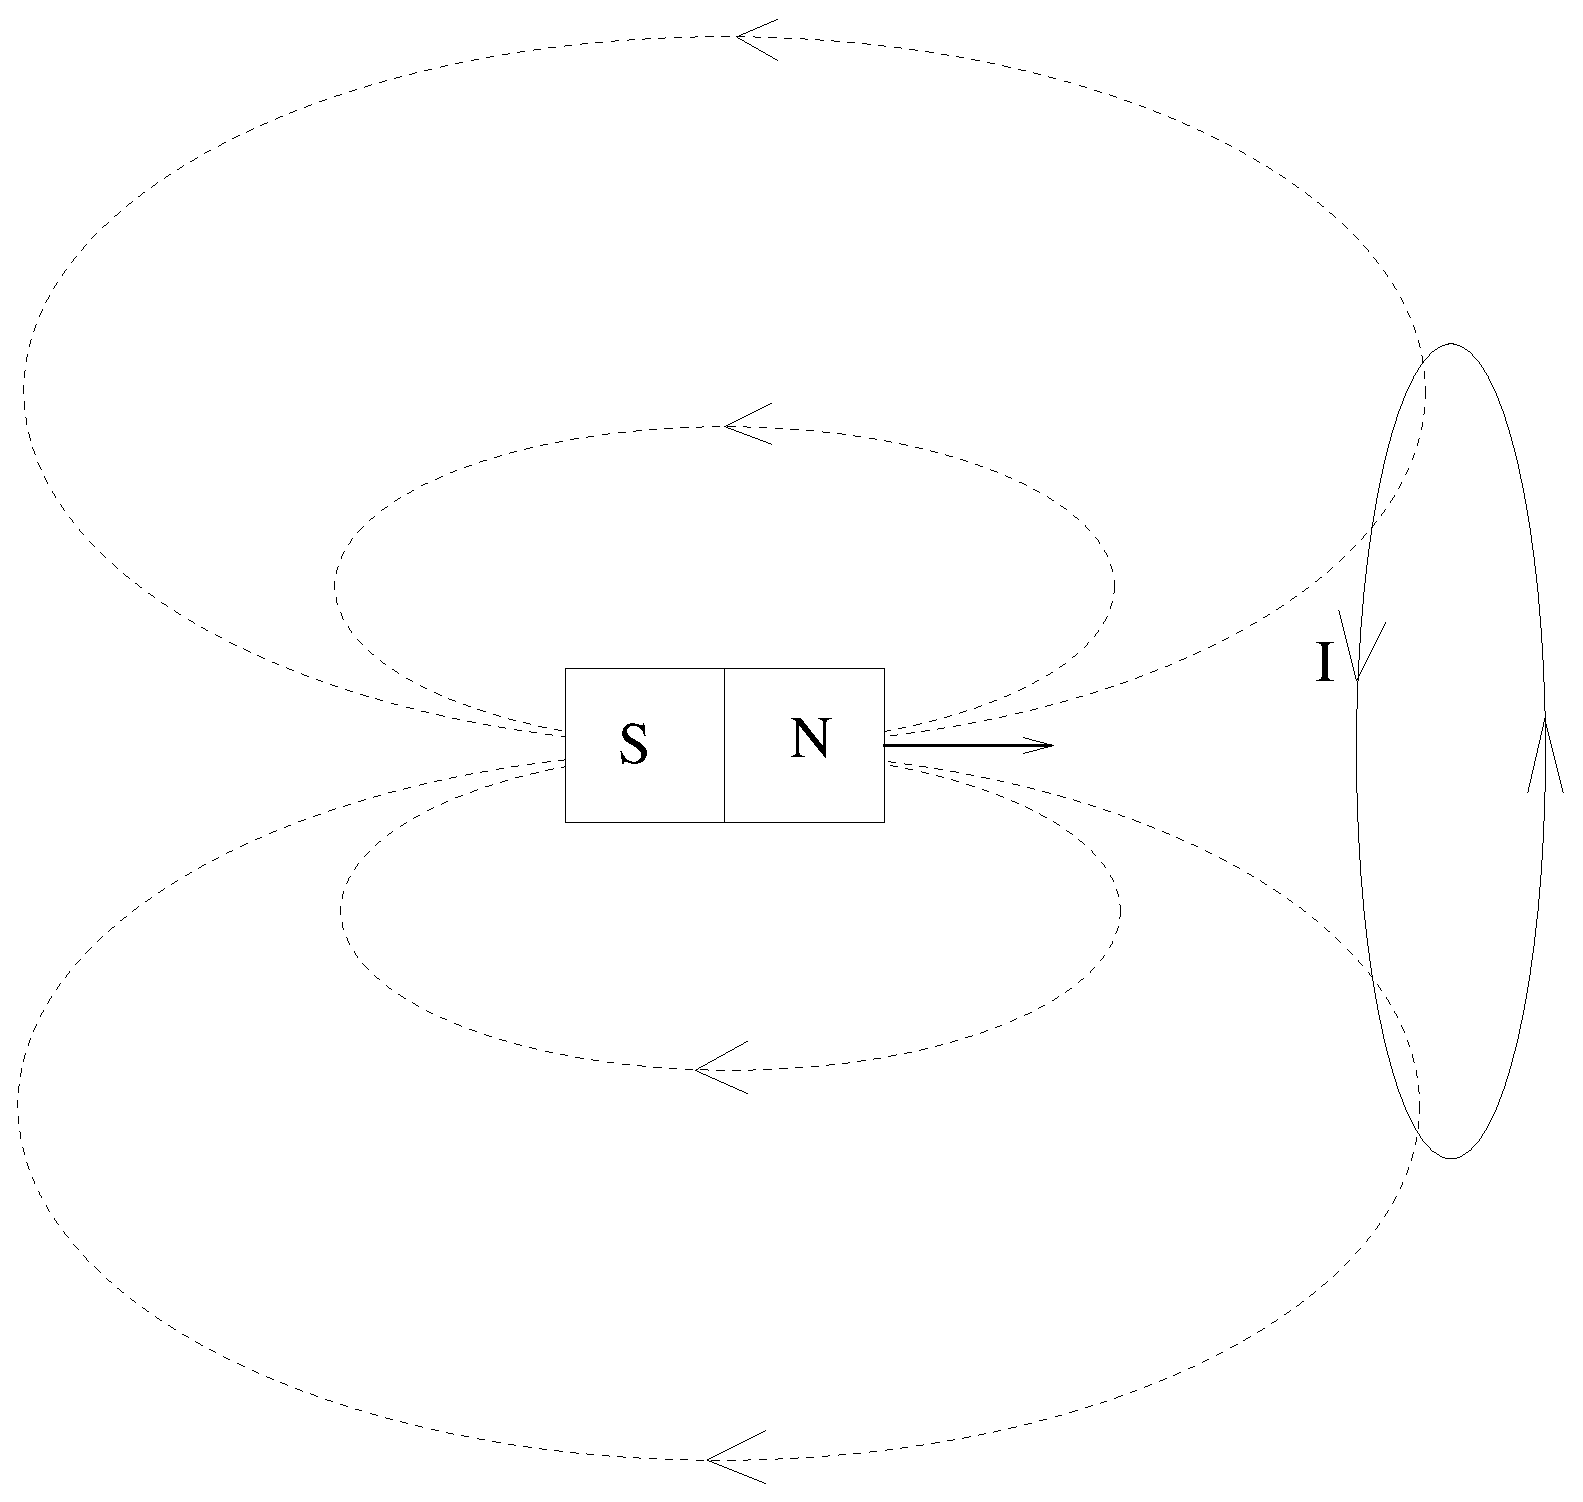
\includegraphics[scale=0.25]{immagini/fisica2/ind_spira01}
\caption{magnete in movimento -- spira ferma.}
\label{magnete_spira}
\end{figure}
Avvicinando una spira percorsa da corrente ad una ferma si genera in quest'ultima una corrente indotta. In generale quando si modifica il flusso del campo magnetico si genera una corrente indotta. La corrente indotta e la relativa fem indotta a sua volta genera un campo magnetico opposto a quello esterno, che si oppone al cambiamento del flusso del campo magnetico.
\section{Legge Faraday--Neumann--Lenz}
\begin{legge}[Faraday--Neumann]
Quando il flusso del vettore induzione magnetica $\ve B$ concatenato con un circuito varia nel tempo, nel circuito si induce una forza elettromotrice proporzionale alla variazione del flusso
\end{legge}
\begin{legge}[Lenz]
In un sistema magnetico ogni variazione produce un'azione che tende ad opporsi alla variazione stessa
\end{legge}
Riassumendo la forza elettromotrice indotta:
\begin{legge}[Faraday--Neumann--Lenz]
\begin{equation}
\mathrm{fem}=-\frac{\ud\Phi(\ve B)}{\ud t}
\end{equation}
\end{legge}
dove il meno tiene conto della legge di Lenz, cioè la corrente indotta $I=\frac{\mathrm{fem}}{R}$ è tale da generare un campo magnetico che annulla la variazione del flusso magnetico totale.

Notare che la $\mathrm{fem}$ esiste anche indipendentemente dalla presenza del circuito, o di un conduttore.
\subsection{Forma differenziale}
Sappiamo che:
\begin{equation}
\mathrm{fem}=\oint_C\ve E\cdot\ud\ve l
\end{equation}
Allora:
\begin{equation}
\mathrm{fem}=-\frac{\ud}{\ud t}\Phi(\ve B)=-\frac{\ud}{\ud t}\int_S\ve B\cdot\ve n\,\ud a=\oint_C\ve E\cdot\ud \ve l
\end{equation}
Se il circuito è indeformabile possiamo portare la deriva sotto il segno di integrale e usando il teorema di Stokes:
\begin{equation}
-\int_S\frac{\partial\ve B}{\partial t}\cdot\ve n\,\ud a=\int_S\ve\nabla\times\ve E\cdot\ve n\,\ud a
\end{equation}
\begin{equation}
\ve\nabla\times\ve E=-\frac{\partial\ve B}{\partial t}
\end{equation}
Se il campo magnetico è variabile nel tempo allora $\rot\ve E\neq 0$, segue che $\ve E$ non è più conservativo.
\section{Flusso tagliato e flusso concatenato}
La legge di Faraday--Neumann--Lenz è una legge sperimentale, non deducibile da altre leggi, tranne in un caso, il flusso tagliato, ovvero quando c'è un moto relativo tra un circuito e una sorgente di campo magnetico.

Consideriamo un circuito rettangolare, in cui un lato sia mobile, in cui ci sia un generatore di corrente continua. Ci sia un campo magnetico perpendicolare alla superficie del circuito. Sulla sbarra mobile agisce una forza di Lorentz:
\begin{equation}
F=IBl
\end{equation}
Per la conservazione dell'energia la potenza del generatore $V_0I$ in parte è dissipata per effetto Joule $RI^2$ e in parte per spostare la sbarra $Fv$:
\begin{equation}
V_0I = RI^2+Fv
\end{equation}
Se la sbarra fosse fissa l'ultimo addendo sarebbe nullo e l'intensità della corrente sarebbe $\frac{V_0}{R}=I_0$, ora invece:
\begin{equation}
\frac{V_0}{R}=I_0=I+\frac{Fv}{I}\frac{1}{R}
\end{equation}
La corrente che circola è inferiore a $I_0$ di:
\begin{equation}
I_0-I=\frac{Fv}{I}\frac{1}{R}
\end{equation}
è come se nel circuito oltre che alla forze elettromotrice $V_0$ agisse una forza elettromotrice $V$ in senso opposto:
\begin{equation}
V=-\frac{Fv}{I}=-lBv=-lB\frac{\ud s}{\ud t}=-\frac{\ud \phi(\ve B)}{\ud t}
\end{equation}
che è la legge di Faraday--Neumann--Lenz.

Nel caso di flusso concatenato invece sia il circuito in cui si induce la corrente sia il circuito sorgente del campo magnetico sono fissi e la variazione del flusso è dovuto a variazioni di corrente nel tempo. Questo caso non è descrivibile con la forza di Lorentz, ma è un caso nuovo.
\section{Autoinduttanza}\index{autoinduttanza|(}
In un circuito isolato il campo magnetico generato dal circuito è funzione della corrente:
\begin{equation}
\ve B=\ve B(I)
\end{equation}
quindi il flusso del campo magnetico:
\begin{equation}
\Phi(\ve B)=\Phi(\ve B(I))
\end{equation}
cioè anch'esso è funzione della corrente la quale è funzione del tempo: $I=I(t)$, allora in questo caso, cioè se la variazione del flusso è data esclusivamente da variazioni di corrente (per esempio il circuito è indeformabile), la legge dell'induzione la possiamo scrivere:
\begin{equation}
\text{fem}=-\frac{\ud\Phi(\ve B)}{\ud t}=-\frac{\ud\Phi(\ve B)}{\ud I}\frac{\ud I}{\ud t}
\end{equation}
\begin{Def}[autoinduttanza di un circuito]
\begin{equation}
L=\frac{\ud\Phi(\ve B)}{\ud I}
\end{equation}
\end{Def}
che è una caratteristica della geometria circuito, infatti:
\[
\ve B(\ve r)=\frac{\mu_0}{4\pi}\int_C I\frac{\ud \ve l\times\left(\ve r-\ve r\,'\right)}{\norm{\ve r-\ve r\,'}^3}
\]
in generale; il flusso:
\[
\Phi(\ve B)=\frac{\mu_0}{4\pi}\int_S I\int_C\frac{\ud \ve l\times\left(\ve r-\ve r\,'\right)}{\norm{\ve r-\ve r\,'}^3}\cdot \ve n\,\ud a
\]
e la derivata nella corrente $\frac{\ud}{\ud I}$:
\[
\frac{\ud\Phi(\ve B)}{\ud I}=\frac{\mu_0}{4\pi}\int_S\int_C\frac{\ud \ve l\times\left(\ve r-\ve r\,'\right)}{\norm{\ve r-\ve r\,'}^3}\cdot \ve n\,\ud a
\]
che dipende solo dalla geometria. La legge di Faraday--Neumann--Lenz in questo caso si scrive:
\begin{equation}
\text{fem}=-L\frac{\ud I}{\ud t}
\end{equation}
L'autoinduttanza si misura in henry\index{henry}:
\[
\henry=\frac{\weber}{\ampere}=\frac{\volt\second}{\ampere}=\ohm\second
\]
\begin{Es}[autoinduttanza di un solenoide\index{autoinduttanza!di un solenoide}]
Vogliamo calcolare l'autoinduttanza di un solenoide di lunghezza $l$, raggio $R$ e con $N$ spire per unità di lunghezza. Il campo magnetico, nell'approssimazione di solenoide infinito sarà 
\begin{equation}
B=
\left\{
\begin{array}{ll}
0&r>R\\
\mu_0NI&r<R
\end{array}
\right.
\end{equation}
Il flusso concatenato con una singola spira circolare risulta:
\begin{equation}
\Phi_\text{spira}=\pi R^2\mu_0NI
\end{equation}
il flusso concatenato con tutto il solenoide, cioè con $Nl$ spire:
\begin{equation}
\Phi=Nl\Phi_\text{spira}=\mu_0N^2\pi R^2 I
\end{equation}
usando la definizione:
\begin{equation}
L=\frac{\ud\Phi}{\ud I}=Nl\Phi_\text{spira}=\mu_0N^2l\pi R^2=\mu_0 N^2 V
\end{equation}
che in realtà vale anche nel caso la sezione non sia circolare essendo il campo magnetico uniforme.
\end{Es}
\begin{Es}[cavo coassiale\index{autoinduttanza!di un cavo coassiale}\index{cavo coassiale}]
Consideriamo un cavo coassiale, cioè due conduttori cilindrici coassiali con raggi $a<b$. I due conduttori sono percorsi da correnti uguali ed opposte. Calcoliamo il campo magnetico all'interno, tra i due cilindri. Consideriamo un cammino chiuso $C$ circolare coassiale coi cilindri di raggio $r:a<r<b$. Allora:
\begin{equation}
\oint_C\ve B\cdot\ud\ve l=\mu I\qquad B=\frac{\mu_0}{2\pi}\frac{I}{r}
\end{equation}
all'esterno del cavo invece la corrente concatenata totale è zero, $B(r>b)=0$. Consideriamo una superficie $S$ rettangolare di larghezza $\Delta l$ con la base inferiore che poggia sul $r=a$ e la base superiore su $r=b$. Il flusso di $\ve B$:
\begin{equation}
\Phi_S(\ve B)=\int_S \ve B\cdot\ve n\,\ud a
\end{equation}
ma $\ve B=B\ver e_\theta$ quindi è ortogonale a $\ve n$:
\begin{equation}
\Phi_S(\ve B)=\int_{a}^{b}\int_{\Delta l} B\,\ud r\ud z=\Delta l\int_a^b\frac{\mu_0I}{2\pi R}\,\ud r=\frac{\mu_0I\Delta l}{2\pi}\log\frac{b}{a}
\end{equation}
\begin{equation}
L=\frac{\ud\Phi}{\ud I}=\frac{\mu_0}{2\pi}\Delta l\log\frac{b}{a}
\end{equation}
l'autoinduttanza per unità di lunghezza è 
\begin{equation}
L=\frac{\mu_0}{2\pi}\log\frac{b}{a}
\end{equation}
\end{Es}
\index{autoinduttanza|)}
\index{mutua induttanza|(}
\section{Mutua induttanza}
Consideriamo $n$ circuiti separati percorsi da correnti. Il circuito $j$ produrrà un campo magnetico $\ve B_j$ il quale concatenerà il circuito $i$ creando un flusso: $\Phi_{ij}$ cioè il flusso sul circuito $i$--esimo creato dal circuito $j$--esimo. Il flusso totale sul circuito $i$ sarà:
\begin{equation}
\Phi_i=\sum_{j=1}^n\Phi_{ij}
\end{equation}
e la forza elettromotrice sul circuito $i$:
\begin{equation}
\text{fem}_i=-\sum_{j=1}^n\frac{\ud\Phi_{ij}}{\ud t}=-\sum_{j=1}^n\frac{\ud\Phi_{ij}}{\ud I_j}\frac{\ud I_j}{\ud t}=-\sum_{j=1}^n M_{ij}\frac{\ud I_j}{\ud t}
\end{equation}
nel caso i circuiti siano indeformabili, cioè se le variazione di flusso siano dovute solo da variazioni di corrente nel tempo.
\begin{Def}[coefficiente di mutua induttanza]
\begin{equation}
M_{ij}=\frac{\ud\Phi_{ij}}{\ud I_j}
\end{equation}
\end{Def}
Naturalmente
\begin{equation}
M_{ii}=L_i
\end{equation}
\subsection{Simmetria di \texorpdfstring{$M$}{M}}
La matrice $M=M_{ij}$ è simmetrica. Dobbiamo dimostrare che $M_{ij}=M_{ji}$. Limitiamoci a considerare due circuiti e dimostriamo $M_{21}=M_{12}$. Il primo circuito genererà un flusso sul secondo:
\begin{equation}
\Phi_2(\ve B_1)=\int_{S_2}\int_{C_1}I_1\frac{\ud l_1\times\left(\ve r_2-\ve r_1\right)}{\norm{\ve r_2-\ve r_1}^3}\cdot n_2\,\ud a_2
\end{equation}
\begin{equation}
M_{21}=\frac{\ud\Phi_2}{\ud I_1}=\int_{S_2}\int_{C_1}\frac{\ud l_1\times\left(\ve r_2-\ve r_1\right)}{\norm{\ve r_2-\ve r_1}^3}\cdot n_2\,\ud a_2
\end{equation}
Usiamo la relazione:
\begin{equation}
\left(\ve A\times\ve B\right)\cdot\ve C=\left(\ve B\times \ve C\right)\cdot\ve A
\end{equation}
\begin{equation}
M_{21}=\int_{S_2}\int_{C_1}\left(\frac{\ve r_2-\ve r_1}{\norm{\ve r_2-\ve r_1}^3}\times\ve n_2\right)\cdot\ud\ve l_1\,\ud a_2
\end{equation}
Usando il teorema del rotore: $\int_C\ve F\cdot\ud \ve l=\int_S\rot\ve F\cdot\ve n_2\,\ud a$:
\begin{equation}
M_{21}=\int_{S_2}\int_{S_1}\rot_1\left(\frac{\ve r_2-\ve r_1}{\norm{\ve r_2-\ve r_1}^3}\times \ve n_2\right)\cdot\ve n_1\,\ud a_1\ud a_2
\end{equation}
Usiamo la relazione:
\begin{equation}
\ve A\times\left(\ve B\times\ve C\right)=\left(\ve A\cdot\ve C\right)\ve B-\left(\ve A\cdot\ve B\right)\ve C
\end{equation}
usando $\ve A=\ve\nabla$:
\begin{equation}
\begin{split}
M_{21}&=\int_{S_2}\int_{S_1}\left[\left(\diver_1\ve n_2\right)\frac{\ve r_2-\ve r_1}{\norm{\ve r_2-\ve r_1}^3}-\left(\diver_1 \frac{\ve r_2-\ve r_1}{\norm{\ve r_2-\ve r_1}^3}\right)\ve n_2\right]\cdot\ve n_1\,\ud a_1\ud a_2\\
&=\int_{S_2}\int_{S_1}-\left(\diver_1 \frac{\ve r_2-\ve r_1}{\norm{\ve r_2-\ve r_1}^3}\right)\ve n_2\cdot\ve n_1\,\ud a_1\ud a_2\\
&=\int_{S_2}\int_{S_1}\left(\diver_2 \frac{\ve r_2-\ve r_1}{\norm{\ve r_2-\ve r_1}^3}\right)\ve n_2\cdot\ve n_1\,\ud a_1\ud a_2\\
&=\int_{S_2}\int_{S_1}\left[\left(\diver_2\ve n_2\right)\frac{\ve r_2-\ve r_1}{\norm{\ve r_2-\ve r_1}^3}+\left(\diver_2 \frac{\ve r_2-\ve r_1}{\norm{\ve r_2-\ve r_1}^3}\right)\ve n_2\right]\cdot\ve n_1\,\ud a_1\ud a_2\\
&=\int_{S_2}\int_{S_1}\rot_2\left(\frac{\ve r_2-\ve r_1}{\norm{\ve r_2-\ve r_1}^3}\times \ve n_2\right)\cdot\ve n_1\,\ud a_1\ud a_2\\
&=\int_{S_1}\int_{C_2}\ud\ve l_2\times\frac{\ve r_2-\ve r_1}{\norm{\ve r_2-\ve r_1}^3}\cdot \ve n_1=M_{21}
\end{split}
\end{equation}
\begin{Es}[trasformatore\index{trasformatore}]
Consideriamo due bobine di lunghezza $l$ e sezione $S$ avvolte su un unico materiale ferromagnetico percorse da correnti $I_1$ e $I_2$. Il campo magnetico $\ve B$ che le attraversa è uguale in modulo. Le due bobine abbiano $N_1$ e $N_2$ spire per unità di lunghezza.
\begin{equation}
B_1=\mu_0N_1I_1\qquad B_2=\mu_0N_2I_2
\end{equation}
Il campo magnetico totale:
\begin{equation}
\ve B=\ve B_1+\ve B_2
\end{equation}
Supponiamo che le due bobine siano messe in modo tale che i due campi siano paralleli:
\begin{equation}
B=B_1+B_2
\end{equation}
\begin{equation}
L_1=\mu_0N_1^2lS\qquad L_2=\mu_0N_2^2lS
\end{equation}
\begin{equation}
M_{12}=\frac{\ud\Phi_2(\ve B_1)}{\ud I_1}=\frac{\ud(\mu_0N_1N_2I_1Sl)}{\ud I_1}=\mu_0N_1N_2Sl
\end{equation}
\begin{equation}
\begin{split}
\text{fem}_1&=-\frac{\ud\Phi(\ve B)}{\ud t}=-\frac{\ud\Phi(\ve B_1+\ve B_2)}{\ud t}=-\frac{\ud\left(\Phi(\ve B_1)+\Phi(\ve B_2)\right)}{\ud t}\\
&=-\frac{\ud\Phi(\ve B_1)}{\ud t}-\frac{\ud\Phi(\ve B_2)}{\ud t}=\frac{\ud\Phi(\ve B_1)}{\ud I_1}\frac{\ud I_1}{\ud t}-\frac{\ud\Phi(\ve B_2)}{\ud I_2}\frac{\ud I_2}{\ud t}\\
&=-L_1\frac{\ud I_1}{\ud t}-M_{12}\frac{\ud I_2}{\ud t}
\end{split}
\end{equation}
analogamente:
\begin{equation}
\text{fem}_2=-L_2\frac{\ud I_2}{\ud t}-M_{21}\frac{\ud I_1}{\ud t}=-L_2\frac{\ud I_2}{\ud t}-M_{12}\frac{\ud I_1}{\ud t}
\end{equation}
\begin{align}
\frac{\text{fem}_1}{\text{fem}_2}&=-\dfrac{L_1\dot I_1+M_{12}\dot I_2}{L_2 \dot I_2+M_{12}\dot I_1}=\frac{\mu_0N_1^2lS\dot I_1+\mu_0N_1N_2Sl\dot I_2}{\mu_0N_2^2lS \dot I_2+\mu_0N_1N_2Sl\dot I_1}\\
&=\frac{N_1^2\dot I_1+N_1N_2\dot I_2}{N_2^2\dot I_2+N_1N_2\dot I_1}=\frac{N_1}{N_2}
\end{align}
\end{Es}
\index{mutua induttanza|)}






\chapter{Circuiti\index{circuiti}}
\minitoc
\begin{Def}[circuito elettrico]
Una rete o circuito elettrico è un insieme di conduttori e generatori di forze elettromotrici collegati tra loro
\end{Def}
\section{Reti resistive}
Una rete resistiva è una rete per la quale compaiono solo componenti passivi resistivi.
\begin{Def}[nodo\index{nodo}]
Un nodo è un punto di connessione tra tre o più elementi della rete
\end{Def}
\begin{Def}[ramo\index{ramo}]
Un ramo è l'insieme degli elementi collegati in serie posti tra due nodi
\end{Def}
\begin{Def}[maglia\index{maglia}]
Una maglia è un percorso chiuso formato da elementi della rete
\end{Def}
Nel risolvere i circuiti, cioè determinare i valori delle correnti che attraversano i componenti o nel determinare la caduta di potenziale su di essi, si usano le leggi di Kirchhoff\index{Kirchhoff}:
\begin{legge}[legge dei nodi]
La somma delle intensità delle correnti entranti in un nodo è uguale alla somma delle intensità delle correnti uscenti
\end{legge}
\begin{legge}[legge delle maglie]
La somma col segno delle forze elettromotrici in un maglia è uguale alla somma delle cadute di tensione di tutti gli elementi della maglia
\end{legge}
La prima legge esprime l'equazione di continuità la seconda la circuitazione del campo elettrostatico.
\section{RLC serie continua}
\subsection{Scarica}
Immaginiamo di aver caricato il condensatore con una carica $q_0$, cui corrisponde una differenza di potenziale tra le armature $\Delta V_0$ e di chiudere il circuito al tempo $t=0$. Per la legge delle maglie:
\begin{equation}
RI(t)+L\frac{\ud I(t)}{\ud t}=\Delta V(t)
\end{equation}
essendo $\Delta V=\frac{q}{C}$:
\begin{equation}
RI+L\frac{\ud I}{\ud t}-\frac{q}{C}=0
\label{LRC_con_q0}
\end{equation}
derivando e tenendo conto che $I=-\frac{\ud q}{\ud t}$ poiché la corrente positiva si genera per diminuzione di $q$ sul condensatore:
\begin{equation}
L\frac{\ud^2I}{\ud t^2}+R\frac{\ud I}{\ud t}+\frac{I}{C}=0
\end{equation}
che è una semplice equazione differenziale omogenea:
\[
L\lambda^2+R\lambda+\frac{1}{C}=0
\]
\[
\lambda_{1/2}=-\frac{R}{2L}\pm\sqrt{\frac{R^2}{4L^2}-\frac{1}{LC}}
\]
Introduciamo la costante di smorzamento:
\begin{equation}
\gamma=\frac{R}{2L}
\end{equation}
e
\begin{equation}
\beta = \sqrt{\frac{R^2}{4L^2}-\frac{1}{LC}}
\end{equation}
la soluzione generale si scrive come
\begin{equation}
I(t)=I_1e^{-(\gamma-\beta)t}+I_2e^{-(\gamma+\beta)t}
\label{soluzione_generale_RLC99}
\end{equation}
a seconda che $\beta$ sia reale, immaginario o nullo si hanno tre casi notevoli:
\begin{itemize}
\item{$\beta=0$}, criticamente smorzato\index{smorzamento critico}. Questo avviene quando:
\begin{equation}
\gamma=\frac{1}{\sqrt{LC}}=\omega_0
\end{equation}
$\omega_0$ è la frequenza caratteristica del circuito. La soluzione diventa:
\begin{equation}
I(t)=(I_1+I_2t)e^{-\gamma t}
\end{equation}
imponendo $I(0)=0$:
\[
I(0)=I_1=0
\]
\begin{equation}
I(t)=I_2 te^{-\gamma t}
\label{LRC_generale01}
\end{equation}
per imporre $q(0)=q_0$ dobbiamo andare a considerare l'equazione \eqref{LRC_con_q0} dove compare ancora $q_0$ prima di derivare. Calcolandola per $t=0$ e considerando $I(0)=0$:
\begin{equation}
L\left.\frac{\ud I}{\ud t}\right|_{t=0}=\frac{q_0}{C}
\label{che_bellissima!}
\end{equation}
andando a sostituire la nostra soluzione generale \eqref{LRC_generale01}:
\begin{equation}
LI_2\left.\left(e^{-\gamma t}-\gamma te^{-\gamma t}\right)\right|_{t=0}=\frac{q_0}{C}\qquad I_2=\frac{q_0}{LC}=q_0\omega_0^2
\end{equation}
che porta alla soluzione particolare:
\begin{equation}
I(t)=q_0\omega_0^2 te^{-\gamma t}
\end{equation}
\item{$\beta>0$} questo avviene quando:
\begin{equation}
\gamma>\omega_0
\end{equation}
e si parla di sottosmorzamento. Imponendo $I(0)=0$ si trova ancora $I_1=-I_2$ quindi:
\begin{equation}
I(t)=I_2\left(e^{-(\gamma+\beta)t}-e^{-(\gamma-\beta)t}\right)
\label{RLC_soluzione_trovata}
\end{equation}
considerando che deve valere ancora la \eqref{che_bellissima!}, sostituendo la soluzione trovata \eqref{RLC_soluzione_trovata}:
\begin{equation}
I_2=-\frac{q_0}{LC}=-\frac{q_0\omega_0^2}{2\beta}
\end{equation}
e la soluzione:
\begin{equation}
I(t)=\frac{q_0\omega_0^2}{2\beta}e^{-\gamma t}\left(e^{\beta t}-e^{-\beta t}\right)
\end{equation}
\item{$\beta\in\field{C}$} che si verifica quando:
\begin{equation}
\gamma<\omega_0
\end{equation}
e si parla di sottosmorzamento. La soluzione generale \eqref{soluzione_generale_RLC99} in questo caso diventa:
\begin{equation}
I(t)=I_1e^{-(\gamma-j \omega)t}+I_2e^{-(\gamma+j \omega)t}
\end{equation}
con $\omega=\sqrt{\frac{1}{LC}-\frac{R^2}{4L^2}}$. Imponiamo $I(0)=0$ che ci fornirà $I_1=-I_2$ e la soluzione diventa:
\begin{equation}
I(t)=I_2\left(e^{-(\gamma+j\omega)t}-e^{-(\gamma-j\omega)t}\right)
\end{equation}
considerando ancora la \eqref{che_bellissima!}
\begin{equation}
I_2=-\frac{q_0}{2Cj\omega L}=\frac{q_0}{2CL\omega}j=\frac{q_0\omega_0^2}{2\omega}j
\end{equation}
e la soluzione
\begin{equation}
I(t)=\frac{q_0\omega_0^2}{2\omega}j\left(e^{-(\gamma+j\omega)t}-e^{-(\gamma-j\omega)t}\right)=\frac{q_0\omega_0^2}{2\omega}j\left(e^{-j\omega t}-e^{j\omega t}\right)e^{-\gamma t}
\end{equation}
poiché
\begin{multline}
j\left[e^{-j\omega t}-e^{j\omega t}\right]=j\left[\left(\cos(-\omega t)+j\sin(-\omega
t)\right)-\left(\cos(\omega t)+j\sin(\omega t)\right)\right]\\
=2\sin(\omega t)
\end{multline}
\begin{equation}
I(t)=\frac{q_0\omega_0^2}{\omega}e^{-\gamma t}\sin(\omega t)
\end{equation}
l'ampiezza delle oscillazioni sinusoidali è smorzata dal termine $e^{-\gamma t}$. Tutta l'energia all'infinito è dissipata per effetto Joule. Il tempo caratteristico dello smorzamento è 
\begin{equation}
\tau=\frac{1}{\gamma}=\frac{2L}{R}
\end{equation}
\end{itemize}
Riassumendo:
\begin{equation}
I(t) = 
\begin{cases}
 \gamma > \omega_0 & \frac{q_0\omega_0^2}{\beta}e^{-t/\tau}\sinh(\beta t) \\
 \gamma = \omega_0 & q_0\omega_0^2te^{-t/\tau}\\
 \gamma < \omega_0 & \frac{q_0\omega_0^2}{\omega}e^{-t/\tau}\sin(\omega t)
\end{cases}
\end{equation}
con $\tau = \frac{1}{\gamma}$ e $\beta=j\omega$.
\subsection{Carica}
Per quanto riguarda la carica dalla legge delle maglie:
\begin{equation}
L\dot I+RI+\frac{Q}{C}=V_0
\end{equation}
la trattazione è del tutto analoga a quella per la scarica:
\begin{itemize}
\item[$\gamma=\omega_0$] smorzamento critico:
\begin{equation}
I(t)=q_0\gamma^2te^{-\gamma t}
\end{equation}
\item[$\gamma>\omega_0$] sovrasmorzamento:
\begin{equation}
I(t)=q_0\frac{\omega_0^2}{2\beta}\left(e^{-(\gamma-\beta)t}-e^{-(\gamma+\beta)t}\right)
\end{equation}
\item[$\gamma<\omega_0$] sottosmorzamento:
\begin{equation}
I(t)=q_0e^{-\gamma t}\left(\gamma\cos(\omega t)+\omega\sin(\omega t)\right)
\end{equation}
\end{itemize}




\section{RLC serie alternata}
Consideriamo un circuito RLC in alternata. Il generatore fornirà ai suoi capi una tensione:
\begin{equation}
V(t)=V_0\cos\left(\omega t\right)=\Re(V_0 e^{j\omega t})
\end{equation}
\subsection{Soluzione stazionaria}
Calcoliamo la soluzione stazionaria, per esempio per $t\to\infty$. Calcoliamo l'impedenza del circuito:
\begin{equation}
Z=Z_R+Z_C+Z_L=R-j\frac{1}{\omega C}+j\omega L=R+j X
\end{equation}
il cui modulo è 
\begin{equation}
|Z|=\sqrt{R^2+\left(\omega L-\frac{1}{\omega C}\right)^2}
\end{equation}
usando i numeri complessi si scrive come:
\begin{equation}
Z=|Z|e^{j\varphi}
\end{equation}
con:
\begin{equation}
\varphi=\arctan\left(\frac{X}{R}\right)=\arctan\left(\frac{\omega L-\frac{1}{\omega C}}{R}\right)
\end{equation}
la corrente che circola nella serie:
\begin{equation}
I(t)=\Re\left({\frac{V(t)}{Z}}\right)=\Re\left({\frac{V_0e^{j\omega t}}{|Z|e^{j\varphi}}}\right)=\Re\left({\frac{V_0}{|Z|}e^{j(\omega t-\varphi)}}\right)=\frac{V_0}{|Z|}\cos(\omega t-\varphi)
\end{equation}
quindi ai capi del resistore avremo una caduta di potenziale:
\begin{equation}
V_R(t)=RI(t)=R\frac{V_0}{|Z|}\cos(\omega t-\varphi)=V_{0R}\cos(\omega t-\varphi)
\end{equation}
con $V_{0R}$ l'ampiezza, pari a:
\begin{equation}
V_{0R}=R\frac{V_0}{|Z|}=\frac{R}{\sqrt{R^2+\left(\omega L-\frac{1}{\omega C}\right)^2}}V_0
\end{equation}
ai capi dell'induttanza (con $Z_L=j\omega L$) una caduta di potenziale:
\begin{equation}
\begin{split}
V_L(t)=&\Re\left(Z_LI(t)\right)=\Re\left(j\omega L\frac{V_0}{|Z|}\cos(\omega t-\varphi)\right)=\Re\left(\omega Le^{j\frac{\pi}{2}}\frac{V_0}{|Z|}e^{j(\omega t-\varphi)}\right)\\
=&\Re\left(\frac{\omega L}{|Z|}V_0e^{\left(\omega t-\varphi+\frac{\pi}{2}\right)}\right)=V_{0L}\cos\left(\omega t-\varphi+\frac{\pi}{2}\right)
\end{split}
\end{equation}
con:
\begin{equation}
V_{0L}=\frac{\omega L}{|Z|}V_0=\frac{\omega L}{\sqrt{R^2+\left(\omega L-\frac{1}{\omega C}\right)^2}}V_0
\end{equation}
mentre ai capi del condensatore ($Z_C=-\frac{j}{\omega C}$):
\begin{equation}
\begin{split}
V_{C}(t)=&\Re(Z_CI(t))=\Re\left(-\frac{j}{\omega C}\frac{V_0}{|Z|}\cos(\omega t-\varphi)\right)=\Re\left(\frac{1}{\omega C}e^{-j\frac{\pi}{2}}\frac{V_0}{|Z|}e^{j(\omega t-\varphi)}\right)\\
=&\Re\left(\frac{1}{|Z|\omega C}V_0e^{j\left(\omega t-\varphi-\frac{\pi}{2}\right)}\right)=V_{0C}\cos\left(\omega t-\varphi-\frac{\pi}{2}\right)
\end{split}
\end{equation}
con:
\begin{equation}
V_{0C}=\frac{1}{|Z|\omega C}V_0=\frac{1}{\omega C\sqrt{R^2+\left(\omega L-\frac{1}{\omega C}\right)^2}}V_0
\end{equation}
Occupiamoci delle ampiezze. Riassumiamo:
\begin{subequations}
\begin{gather}
V_{0R}=\frac{R}{\sqrt{R^2+\left(\omega L-\frac{1}{\omega C}\right)^2}}V_0\\
V_{0L}=\frac{\omega L}{\sqrt{R^2+\left(\omega L-\frac{1}{\omega C}\right)^2}}V_0\\
V_{0C}=\frac{1}{\omega C\sqrt{R^2+\left(\omega L-\frac{1}{\omega C}\right)^2}}V_0\\
I_0=\frac{V_0}{\sqrt{R^2+\left(\omega L-\frac{1}{\omega C}\right)^2}}
\end{gather}
\end{subequations}
Vogliamo trovare qual è quella frequenza $\nu_0$ che rende massima la corrente:
\[
\left.\frac{\ud}{\ud \omega}I_0\right|_{\omega=\omega_0}\!\!\!\!\!\!\!\!=0\qquad
\left(R^2+\left(\omega_0 L-\frac{1}{\omega_0 C}\right)^2\right)^{-\frac{3}{2}}\left(\omega_0 L-\frac{1}{\omega_0 C}\right)\left(L+\frac{1}{\omega_0 ^2 C}\right)=0
\]
\begin{equation}
\omega_0=\frac{1}{\sqrt{LC}}\qquad \nu_0=\frac{1}{2\pi\sqrt{LC}}
\end{equation}
che è effettivamente un massimo (la derivata seconda in $\omega_0$ vale $-\frac{4L^2}{R^2}$). Quando $\omega=\omega_0$ si parla di risonanza del circuito.
Possiamo anche valutare quando abbiamo i massimi per $V_{0L}$ e $V_{0C}$:
\begin{equation}
\omega_{0C}=\frac{\sqrt{-2C(R^2C-2L)}}{2CL}
\end{equation}
\begin{equation}
\omega_{0L}=\frac{2}{\sqrt{-2R^2C^2+4CL}}
\end{equation}
Il valore massimo per l'ampiezza del potenziale nell'induttanza è uguale a quello per il capacitore:
\begin{equation}
V_{0L}(\omega_{0L})=V_{0C}(\omega_{0C})=\frac{2L}{\sqrt{C}\sqrt{-CR^2+2L}R\sqrt{\frac{4L-CR^2}{-CR^2+2L}}}V_0
\end{equation}
mentre naturalmente il valore massimo che assume $V_{0R}$ è 
\begin{equation}
V_{0R}(\omega_0)=V_0
\end{equation}
quando $\omega=\omega_0$ $V_{0L}$ e $V_{0C}$ sono uguali:
\begin{equation}
V_{0L}(\omega_0)=V_{0C}(\omega_0)=\frac{\sqrt{L}}{\sqrt{C}R}V_0
\end{equation}
per quanto riguarda i limiti:
\begin{subequations}
\begin{align}
&\lim_{\omega\to 0^+}V_{0R}=0&\lim_{\omega\to \infty}V_{0R}=0\\
&\lim_{\omega\to 0^+}V_{0L}=0&\lim_{\omega\to \infty}V_{0L}=V_0\\
&\lim_{\omega\to 0^+}V_{0C}=V_0&\lim_{\omega\to \infty}V_{0C}=0
\end{align}
\end{subequations}

Per quanto riguarda le differenze di fase dei potenziali rispetto al potenziale del generatore:
\begin{subequations}
\begin{gather}
\phi_R=\varphi=\arctan\left(\frac{\omega L-\frac{1}{\omega C}}{R}\right)\\
\phi_L=\varphi-\frac{\pi}{2}=\arctan\left(\frac{\omega L-\frac{1}{\omega C}}{R}\right)-\frac{\pi}{2}\\
\phi_C=\varphi+\frac{\pi}{2}=\arctan\left(\frac{\omega L-\frac{1}{\omega C}}{R}\right)+\frac{\pi}{2}
\end{gather}
\end{subequations}
Cerchiamo il caso in cui non si ha sfasamento ai capi del resistore rispetto al generatore:
\[
0=\phi_R=\arctan\left(\frac{\omega L-\frac{1}{\omega C}}{R}\right)
\]
\begin{equation}
\omega=\frac{1}{\sqrt{LC}}=\omega_0
\end{equation}
quindi solo alla frequenza di risonanza non si ha sfasamento sul resistore. I limiti:
\begin{subequations}
\begin{align}
&\lim_{\omega\to 0^+}\phi_R=-\frac{\pi}{2}&\lim_{\omega\to\infty}\phi_R=\frac{\pi}{2}\\
&\lim_{\omega\to 0^+}\phi_L=-\pi&\lim_{\omega\to\infty}\phi_L=0\\
&\lim_{\omega\to 0^+}\phi_C=0&\lim_{\omega\to\infty}\phi_C=\pi
\end{align}
\end{subequations}
\begin{figure}[htbp]
\centering
\includegraphics[scale=0.45]{immagini/fisica2/RLC_01}
\caption{Andamento delle ampiezze in funzione della frequenza e differenze di fase in funzione delle frequenza.}
\end{figure}
Introduciamo la grandezza coefficiente di smorzamento $\gamma$:
\begin{equation}
\gamma = \frac{R}{2L}
\end{equation}
e il fattore di merito o di qualità $Q_0$:
\begin{equation}
Q_0 = {\omega_0L}{R}=\frac{\omega_0}{2\gamma}
\end{equation}
Dividiamo in tre casi notevoli:
\begin{itemize}
\item[$\omega=\omega_0$]
\begin{gather}
Z = \left[R-j\frac{1}{\omega C}+j\omega L\right]_{\omega=\omega_0}=R\\
\varphi = \left[\arctan\left(\frac{X}{R}\right)\right]_{X=0}=0\\
I = \frac{V_0}{|Z|}\cos\left(\omega t-\varphi\right)=\frac{V_0}{R}\cos(\omega t)=I_0\cos(\omega t)\\
V_{0R}=V_0\\
V_{0L}=I_0|Z_L|=\frac{V_0}{R}\omega_0 L=\frac{\omega_0}{2\gamma}V_0=Q_0V_0\\
V_{0C}=I_0|Z_C|=\frac{V_0}{R}\frac{1}{\omega_0 C}=\frac{\omega_0}{2\gamma}V_0=Q_0V_0
\end{gather}
\item[$\omega\ll\omega_0$]
\begin{gather}
Z=R-j\frac{1}{\omega C}+j\omega L\simeq -\frac{1}{\omega C}j\\
\varphi \simeq \left[\arctan\left(\frac{X}{R}\right)\right]_{R=0^+,X<0}=-\frac{\pi}{2}\\
I_0 = \frac{V_0}{|Z|}=\omega C V_0\\
V_{0R}\simeq I_0R=R\omega C V_0=\frac{\omega}{\omega_0}\frac{V_0}{Q_0}\\
V_{0L}\simeq I_0|Z_L|=\omega^2LCV_0=\frac{\omega^2}{\omega_0^2}V_0\\
V_{0C}\simeq I_0|Z_C|=\omega C V_0\frac{1}{\omega C}=V_0
\end{gather}
\item[$\omega\gg\omega_0$]
\begin{gather}
Z=R-j\frac{1}{\omega C}+j\omega L\simeq j\omega L\\
\varphi \simeq \left[\arctan\left(\frac{X}{R}\right)\right]_{R=0^+,X>0}=+\frac{\pi}{2}\\
I_0 = \frac{V_0}{|Z|}= \frac{V_0}{\omega L}\\
V_{0R}\simeq I_0R=\frac{R}{\omega L}V_0=\frac{2\gamma}{\omega}V_0=\frac{\omega_0}{\omega}\frac{V_0}{Q}\\
V_{0L}\simeq I_0|Z_L|=\frac{V_0}{\omega L}\omega L=V_0\\
V_{0C}\simeq I_0|Z_C|=\frac{V_0}{\omega L}\frac{1}{\omega C}=\frac{1}{\omega^2 LC}V_0=\frac{\omega_0^2}{\omega^2}V_0
\end{gather}
\end{itemize}
\subsubsection{Ampiezza di banda}
La frequenza $\omega_0$ è un punto, che essendo un punto è impossibile da raggiungere. Quello che vogliamo è che il massimo della caduta di potenziale sulla resistenza sia ``largo'' in modo tale che se la nostra frequenza non è precisamente $\omega_0$ abbiamo lo stesso risonanza. Scriviamo l'intensità di corrente in funzione di $Q_0=\frac{\omega_0L}{R}$:
\begin{equation}
I_0=\frac{V_0}{|Z|}=\frac{\frac{V_0}{R}}{\sqrt{1+Q_0^2\left(\frac{\omega^2-\omega_0^2}{\omega\omega_0}\right)^2}}
\end{equation}
mentre l'ampiezza della caduta sul resistore:
\begin{equation}
V_{0R}=I_0R=\frac{V_0}{|Z|}R=\frac{R}{|Z|}V_0
\end{equation}
interessante è il rapporto:
\begin{equation}
\frac{R}{|Z|}=\frac{1}{\sqrt{1+Q_0^2\left(\frac{\omega^2-\omega_0^2}{\omega\omega_0}\right)^2}}
\end{equation}
Indichiamo con $\omega_1$ e $\omega_2$ i punti di potenza dimezzata, cioè quei valori per cui il valore del rapporto $\frac{R}{|Z|}$ diventa $\frac{1}{\sqrt{2}}$ del suo massimo. Il massimo si ha quando $\omega=\omega_0$ e il valore massimo vale $1$. Quindi la condizione si ha quando:
\begin{equation}
Q_0^2\left(\frac{\omega^2-\omega_0^2}{\omega\omega_0}\right)^2=1
\end{equation}
le soluzioni positive sono:
\begin{equation}
\omega_{1,2}=\frac{\pm+\sqrt{\omega_0^2+4Q_0^2\omega_0^2}}{2Q_0}
\end{equation}
quindi l'ampiezza di banda $\Delta\omega$:
\begin{equation}
\Delta\omega=\omega_1-\omega_2=\frac{\omega_0}{Q_0}
\end{equation}
inversamente proporzionale a $Q_0$\footnote{$Q_0$ è chiamato fattore di merito perché nelle applicazioni è utile avere un'ampiezza di banda stretta e quindi un $Q_0$ alto; spesso i resistori nei circuiti RLC non sono presenti e la resistenza è data dall'avvolgimento dell'induttanza e quindi $Q_0$ diventa un parametro relativo all'induttanza}.

\subsection{Soluzione transitoria}
Supponiamo che il generatore venga acceso all'istante $t=0$. Per la seconda legge di Kirchhoff:
\begin{equation}
\varepsilon=RI+L\frac{\ud I}{\ud t}+\frac{q}{C}
\end{equation}
derivando:
\begin{equation}
\frac{\ud \varepsilon}{\ud t}=R\frac{\ud I}{\ud t}+L\frac{\ud^2 I}{\ud t^2}+\frac{I}{C}
\end{equation}


\section{Cavi coassiali}
Il cavo coassiale\index{cavo!coassiale} è costituito da filo conduttore coassiale con un conduttore cilindrico cavo. Tra i due conduttori è posto del dielettrico.
\subsection{Propagazione dell'onda}
Sia $a$ il raggio del conduttore interno, $b$ quello del dielettrico con permeabilità magnetica trascurabile ($\mu_r\simeq 1$) e permittività dielettrica relativa $\epsilon_r$. Lavoriamo con l'approssimazione di cavo infinito e orientiamo il cavo in modo che abbia l'asse $z$ coassiale. Consideriamo:
\begin{equation}
\diver\ve D=\rho
\end{equation}
e una superficie cilindrica $S$ coassiale, con basi di raggio $r$ e di coordinate $z$ e $z+\Delta z$ (Fig.\ref{coassiali_01})
\begin{figure}[htbp]
\centering
\includegraphics[scale=0.5]{immagini/fisica2/coassiali_01}
\caption{cavo coassiale.}
\label{coassiali_01}
\end{figure}
Calcoliamo $\ve D$, che per simmetria è radiale. Con Gauss $D2\pi r\Delta z=q=\lambda\Delta z$
\begin{equation}
\ve D(z,t)=\frac{\lambda(z,t)}{2\pi r}
\label{lambda_coa}
\end{equation}
con $\lambda$ densità lineare di carica.

Usiamo ora l'equazione:
\begin{equation}
\rot\ve H=\ve J+\frac{\partial\ve D}{\partial t}
\end{equation}
e consideriamo un cammino circolare di raggio $r$ coassiale, perpendicolare a $z$ e la superficie $S$ che lo delimita \ref{coassiali_02}.
\begin{figure}[htbp]
\centering
\includegraphics[scale=0.5]{immagini/fisica2/coassiali_02}
\caption{sezione di cavo coassiale.}
\label{coassiali_02}
\end{figure}
\begin{equation}
\int_S\rot\ve H\cdot \ve n\,\ud a=\int_S\ve J\cdot\ve n\,\ud a+\int_S\frac{\partial\ve D}{\partial t}\cdot \ve n\,\ud a=\oint_C\ve H\cdot\ud\ve l=2\pi r H
\end{equation}
ma $\ve D\cdot\ve n=0$ perché $\ve D=D\ver {e_r}$ e $\int_S\ve J\cdot\ve n\,\ud a=I$. Allora:
\begin{equation}
H(z,t)=\frac{I(z,t)}{2\pi r}
\end{equation}
con $I$ la corrente che scorre nel cavo interno.

Consideriamo ora un circuito rettangolare posto nel piano radiale di lati $\Delta r$ e $\Delta z$ (fig. \ref{coassiali_03}).
\begin{figure}[htbp]
\centering
\includegraphics[scale=0.5]{immagini/fisica2/coassiali_03}
\caption{percorsi.}
\label{coassiali_03}
\end{figure}
Usiamo l'equazione:
\begin{equation}
\rot\ve E=-\frac{\partial\ve B}{\partial t}
\end{equation}
Facendo il flusso e applicando Stokes:
\begin{equation}
\oint_{C}\ve E\cdot\ud \ve l=-\frac{\ud}{\ud t}\int_{S}\ve B\cdot\ve n\,\ud a
\end{equation}
ovvero (approssimando $\ve E(z+\Delta z)=\ve E(z)+\frac{\partial\ve E(z)}{\partial z}\Delta z$):
\begin{equation}
\left[E(z,t)+\frac{\partial E}{\partial z}\Delta z\right]\Delta r-E(z,t)\Delta r=-\frac{\partial B}{\partial t}\Delta z\Delta t
\end{equation}
Semplificando:
\begin{equation}
\frac{\partial E}{\partial z}-\frac{\partial B}{\partial t}
\label{coa_dif1}
\end{equation}
Se ora usiamo il circuito $C_2$ posto in un piano perpendicolare alla direzione radiale e usiamo
\begin{equation}
\rot \ve H=\ve J+\frac{\partial \ve{D}}{\partial t}
\end{equation}
Facendo attenzione ai segni e alle direzioni delle normali e notando che $\ve J$ è parallelo alla superficie:
\begin{equation}
H(z)\Delta r-\left[H(z)-\frac{\partial H}{\partial z}\Delta z\right]\Delta r=\frac{\partial D}{\partial t}\Delta r\Delta z
\end{equation}
ovvero:
\begin{equation}
\frac{\partial H}{\partial z}=-\frac{\partial D}{\partial t}
\label{coa_dif2}
\end{equation}

Derivando la \eqref{coa_dif1} rispetto a $z$, usando la \eqref{coa_dif2}, e $\ve B=\mu\ve H$ e $\ve D=\varepsilon\ve E$:
\begin{equation}
\frac{\partial^2 E}{\partial z^2}=-\frac{\partial}{\partial z}\left(\frac{\partial B}{\partial t}\right)=-\mu\frac{\partial}{\partial t}\left(\frac{\partial H}{\partial z}\right)=\mu\frac{\partial}{\partial t}\left(\frac{\partial D}{\partial t}\right)=\varepsilon\mu\frac{\partial^2 E}{\partial t^2}
\end{equation}
se invece facciamo la stessa cosa partendo dalla \eqref{coa_dif2}:
\begin{equation}
\frac{\partial^2 H}{\partial z^2}=-\frac{\partial}{\partial z}\left(\frac{\partial D}{\partial t}\right)=-\varepsilon\frac{\partial}{\partial t}\left(\frac{\partial E}{\partial z}\right)=\varepsilon\frac{\partial}{\partial t}\left(\frac{\partial B}{\partial t}\right)=\varepsilon\mu\frac{\partial^2 H}{\partial t^2}
\end{equation}
Che è l'equazione di un'onda con velocità 
\begin{equation}
v=\frac{1}{\sqrt{\varepsilon\mu}}
\end{equation}
Usando la \eqref{lambda_coa}: $D(z,t)=\frac{\lambda(z,t)}{2\pi r}$:
\begin{equation}
\frac{\partial^2\lambda}{\partial z^2}=\frac{1}{v^2}\frac{\partial^2 \lambda}{\partial t^2}
\end{equation}
e la soluzione è del tipo:
\begin{equation}
\lambda(z,t)=\psi(z\pm vt)
\end{equation}

Ipotizziamo che all'estremità del cavo sia applicata una differenza di potenziale $V$:
\begin{equation}
V = \varphi(t)
\end{equation}
fissando $z$ la differenza di potenziale tra il conduttore esterno e quello interno vale:
\begin{equation}
V(z,t)=\int_a^b\ve E\cdot\ud\ve r=\int_a^b\frac{1}{\varepsilon}\ve D\cdot\ud\ve r=\int_a^b\frac{\lambda(z,t)}{2\varepsilon\pi r}\,\ud r=\frac{\lambda(z,t)}{2\pi\varepsilon}\log\frac{b}{a}
\end{equation}
la quantità $\frac{2\pi\varepsilon}{\log\frac{b}{a}}$ è la capacità $C$ per unità di lunghezza di un condensatore cilindrico, come un questo caso.
\begin{equation}
V(z,t)=\frac{\lambda(z,t)}{C}
\end{equation}
quindi anche la differenza di potenziale è un'onda. Inoltre anche la corrente $I$ rispetta l'equazione delle onde.
\subsection{Rappresentazione a elementi concentrati}
Si può dimostrare che un cavo coassiale si comporta come un circuito formato dal ripertersi di una certa combinazione di elementi concentrati.

La resistenza $R$ per unità di lunghezza tiene conto della perdita di tensione sul cavo. La capacità $C$ per unità di lunghezza è quella del cilindro, usata nel paragrafo precedente. La conduttanza $G$ tiene conto delle perdite sul condensatore attraverso il dielettrico.
\subsection{Impedenza caratteristica}
L'impedenza caratteristica $Z_0$ è quell'impedenza tale che inserita come carico risulta uguale all'impedenza della linea.
\begin{equation}
Z_0=\frac{Z_1}{2}+\left[\frac{1}{Z_2}+\frac{1}{\frac{Z_1}{2}+Z_0}\right]^{-1}
\end{equation}
\begin{equation}
Z_0=\sqrt{\left(\frac{Z_1}{2}\right)^2+Z_2Z_1}
\end{equation}
\begin{equation}
Z_0=\sqrt{\frac{R+j\omega L}{G+j\omega C}+\left(R+j\omega L\right)^2\frac{(\Delta x)^2}{4}}
\end{equation}
ma gli elementi sono concentrati, quindi $\Delta x\to 0$:
\begin{equation}
Z_0=\sqrt{\frac{R+j\omega L}{G+j\omega C}}
\end{equation}
Una linea non dissipativa è tale che $R=0$ e $G=0$, quindi:
\begin{equation}
{Z_0}_\text{non dissipativa}=\sqrt{\frac{L}{C}}
\end{equation}
in questo caso l'impedenza è reale. Un altro caso in cui l'impedenza è reale è il caso di linea bilanciata:
\begin{equation}
\frac{R}{L}=\frac{G}{C}
\end{equation}
\begin{equation}
{Z_0}_\text{bilanciata}=\sqrt{\frac{L}{C}}
\end{equation}













\chapter{Campo elettromagnetico}
\minitoc
Riassumiamo i risultati finora ottenuti. Le relazioni costitutive della materia descrivono ogni materiali dal punto di vista di conduttore, dielettrico e magnetico:
\begin{subequations}
\begin{gather}
\ve J=\ten\sigma\ve E\\
\ve D=\ten\varepsilon\ve E\\
\ve B=\ten\mu\ve H
\end{gather}
\end{subequations}
A queste vanno aggiunte le equazioni di Maxwell fin'ora ricavate:
\begin{subequations}
\begin{gather}
\diver\ve D=\rho\\
\rot\ve E=-\frac{\partial\ve B}{\partial t}\\
\diver\ve B=0\\
\rot\ve H=\ve J
\end{gather}
\end{subequations}
Hanno una struttura asimmetrica, soprattutto nei rotori, se il rotore di $\ve E$ è influenzato dalla variazione di $\ve B$ nel tempo ci si aspetterebbe che anche il rotore di $\ve B$ sia influenzato dalla variazione di $\ve E$ nel tempo. Sappiamo dall'equazione di continuità
\begin{equation}
\diver\ve J+\frac{\partial\rho}{\partial t}=0
\end{equation}
vediamo se è compatibile con le equazioni di Maxwell.
\begin{equation}
\diver\ve J=\diver\rot\ve H=0\neq -\frac{\partial\rho}{\partial t}
\end{equation}
perché la divergenza di un rotore è sempre nulla. L'equazione di continuità non è compatibile con le nostre equazioni. \`E compatibile se e solo se $\diver\ve J=0$ cioè se $\frac{\partial\rho}{\partial t}=0$ ovvero se la corrente è stazionaria. Concludiamo che le relazioni fino ad ora esposte valgono solo nel caso stazionario.
\section{Corrente di spostamento}
\begin{figure}[htbp]
\centering
\includegraphics[scale=0.9]{immagini/fisica2/faraday_spo}
\end{figure}
Facciamo il ragionamento di Faraday\index{Faraday}. Come è possibile che la corrente passi in un condensatore essendoci tra le due lastre un dielettrico non conduttore, al limite il vuoto? Immaginiamo un condensatore. Sia $S_1$ una superficie piana, ortogonale al verso della corrente entrante che la concatena. Sia $S_2$ invece una superficie che poggia su $S_1$ e che concatena la regione tra le armature. Calcoliamo le circuitazioni di $\ve H$ lungo i bordi della superfici (che coincidono) con il teorema di ampere:
\begin{equation}
\oint_C\ve H\cdot\ud\ve l=\int_{S_1}\ve J\cdot\ve n\,\ud a=I
\end{equation}
perché concatena la corrente $I$, usando l'altra superficie:
\begin{equation}
\oint_C\ve H\cdot\ud\ve l=\int_{S_2}\ve J\cdot\ve n\,\ud a=0
\end{equation}
C'è una contraddizione. Faraday introduce le correnti di spostamento $\ve J_s$ che chiudono il circuito. Essendo $\diver\ve D=\rho$ allora in questo caso, all'interno del condensatore:
\[
D=\sigma(t)
\]
con $\sigma$ la densità di carica sulle armature del condensatore. Il flusso all'interno del condensatore:
\[\phi(\ve D)=S\sigma(t)=q(t)\]
Derivando nel tempo:
\[\frac{\partial\phi(\ve D)}{\partial t}=\frac{\ud q}{\ud t}(t)=I(t)\]
\[\frac{\partial\ve D}{\partial t}=\ve J_S\]

\subsection{Calcolo correnti di spostamento}
Partiamo dall'equazione di continuità che sicuramente è giusta:
\begin{equation}
\diver\ve J=-\frac{\partial\rho}{\partial t}=-\frac{\partial}{\partial t}\diver\ve D=-\diver\frac{\partial\ve D}{\partial t}
\end{equation}
Portando tutto in un'unica divergenza:
\begin{equation}
\diver\left(\ve J+\frac{\partial\ve D}{\partial t}\right)=0
\end{equation}
Il termine in più che è comparso è la corrente di spostamento:
\begin{equation}
\frac{\partial\ve D}{\partial t}=\ve J_S
\end{equation}
L'equazione di Ampere diventa allora:
\begin{equation}
\rot\ve H=\ve J+\frac{\partial\ve D}{\partial t}
\end{equation}
che soddisfa anche il caso stazionario, perché $\frac{\partial\ve D}{\partial t}=0$ e ci si riconduce all'equazione precedente.
\section{Equazioni di Maxwell complete}
Le equazioni di Maxwell che descrivono tutto l'elettromagnetismo sono diventate:\footnote{nel sistema CGS doppio simmetrico di Gauss le stesse equazioni si scrivono come:
\begin{gather*}
\diver\ve D=4\pi\rho\\
\rot\ve E=-\frac{1}{c}\frac{\partial\ve B}{\partial t}\\
\diver\ve B =0\\
\rot\ve H=\frac{1}{c}\frac{\partial\ve{D}}{\partial t}+\frac{4\pi}{c}\ve J\\
\end{gather*}
}
\begin{subequations}
\begin{gather}
\diver\ve D=\rho\\
\rot\ve E=-\frac{\partial\ve B}{\partial t}\\
\diver\ve B=0\\
\rot\ve H=\ve J+\frac{\partial\ve D}{\partial t}
\end{gather}
\end{subequations}
considerando anche le relazioni costitutive abbiamo 16 incognite e 17 equazioni, le equazioni non sono indipendenti; possiamo considerare indipendenti quelle che contengono le sorgenti $\rho$, $\ve J$:
\begin{gather}
\diver\ve D=\rho\\
\rot\ve H=\ve J+\frac{\partial\ve D}{\partial t}
\end{gather}
L'ultima può essere riscritta tenendo conte che $\ve D=\varepsilon_0\ve E+\ve P$:
\begin{equation}
\rot\ve H=\varepsilon_0\frac{\partial\ve E}{\partial t}+\frac{\partial\ve P}{\partial t}+\ve J
\end{equation}
Si notano tre densità di correnti, una di cariche libere $\ve J$, mentre la corrente di spostamento è divisa in $\varepsilon_0\frac{\partial\ve E}{\partial t}$ e $\frac{\partial\ve P}{\partial t}$ che è presente solo nei dielettrici.
\subsection{Equazione di continuità}
L'equazione di continuità è già contenuta nelle equazioni di Maxwell:
\begin{equation}
\diver\rot\ve H=\diver\left(\ve J+\frac{\partial\ve D}{\partial t}\right)=
\diver\ve J+\frac{\partial}{\partial t}\diver\ve D=\diver\ve J+\frac{\partial\rho}{\partial t}=0
\end{equation}
\section{Conservazione dell'energia elettromagnetica}
Consideriamo un volume $V$ contenuto nella superficie $S$ all'interno del quale ci sia un campo elettrico $\ve E(\ve r,t)$ e un campo magnetico $\ve B(\ve r,t)$ variabili nel tempo. Sia $N$ il numero di cariche $q$ per unità di volume con velocità $v$, la forza nell'unità di volume sulle cariche è 
\begin{equation}
\ve f=\frac{\ud\ve F}{\ud V}=Nq\left(\ve E+\ve v\times\ve B\right)
\end{equation}
La potenza nel volume:
\begin{equation}
\begin{split}
\ve f\cdot\ve v&=\frac{\ud P_J}{\ud V}=Nq\left(\ve E+\ve v\times\ve B\right)\cdot\ve v=Nq\ve E\cdot\ve v+Nq\ve v\cdot\left(\ve v\times\ve B\right)\\
&=Nq\ve v\cdot\ve E=\ve J\cdot\ve E
\end{split}
\end{equation}
Come doveva essere il campo magnetico non compie lavoro. La potenza dissipata per effetto Joule la ricaviamo integrando:
\begin{equation}
P_J=\int_V\ve J\cdot\ve E\,\ud v
\end{equation}
Essendo $\ve J=\rot\ve H-\frac{\partial\ve D}{\partial t}$ e usando:
\[
  \diver\left(\ve E\times\ve H\right)=\ve H\cdot\rot\ve E-\ve E\cdot\rot\ve H
\]
\begin{equation}
\begin{split}
P_J&=\int_V\ve J\cdot\ve E\,\ud v=\int_V\left(\ve E\rot\ve H-\ve E\cdot\frac{\partial\ve D}{\partial t}\right)\,\ud v\\
&=-\int_V\diver\left(\ve E\times\ve H\right)\,\ud v+\int_V\ve H\rot\ve E\,\ud v-\int_V\ve E\cdot\frac{\partial\ve D}{\partial t}\,\ud v\\
&=-\int_S\left(\ve E\times\ve H\right)\cdot\ve n\,\ud a-\int_V\left(\ve H\cdot\frac{\partial\ve B}{\partial t}+\ve E\cdot\frac{\partial\ve D}{\partial t}\right)\,\ud v\\
&=-\int_S \ve S\cdot\ve n\,\ud a-\int_V\left(\frac{\partial}{\partial t}\left(\frac{1}{2}\left(\ve H\cdot\ve B\right)+\frac{1}{2}\left(\ve E\cdot\ve D\right)\right)\right)\ud v
\end{split}
\end{equation}
Avendo usato il teorema della divergenza, definito il vettore di Poynting\index{Poynting}\index{vettore!di Poyning}:
\begin{equation}
\ve S=\ve E\times\ve H
\end{equation}
che si misura in \watt\per\meter\squared. Nell'ultimo passaggio abbiamo usato:
\begin{equation}
\frac{1}{2}\frac{\partial}{\partial t}\left(\ve E\cdot\ve D\right)=\frac{1}{2}\frac{\partial}{\partial t}\left(\varepsilon E^2\right)=\ve E\cdot\frac{\partial\ve D}{\partial t}
\end{equation}
e analogamente:
\begin{equation}
\frac{1}{2}\frac{\partial}{\partial t}\left(\ve H\cdot\ve B\right)=\ve H\cdot\frac{\partial\ve B}{\partial t}
\end{equation}
Essendo $w_e=\ve E\cdot\ve D$ l'energia elettrica e $w_h=\ve H\cdot\ve B$ quella magnetica si ha:
\begin{equation}
P_J=-\int_S\ve S\cdot\ve n\,\ud a-\int_V\frac{\partial}{\partial t}{w_{em}}\,\ud v=-\int_S\ve S\cdot\ve n\,\ud a-\frac{\partial}{\partial t}{W_{em}}\,\ud v
\end{equation}
con $w_{em}=w_e+w_h$ la densità di energia elettromagnetica. Si ottiene infine:
\begin{equation}
\frac{\partial W_{em}}{\partial t}=P_J+\int_S\ve S\cdot\ve n\,\ud a
\end{equation}
dove $W_{em}$ è l'energia elettromagnetica. Si deduce che la potenza è dissipata per due fattori: l'effetto Joule $P_J$ e l'irraggiamento attraverso la superficie.
\section{Quantità di moto elettromagnetica}
In un sistema meccanico isolato la quantità di moto $\ve{G^M}$ è una costante del moto e vale:
\begin{equation}
\ve F=\frac{\ud \ve{G^M}}{\ud t}
\end{equation}
in un sistema elettromagnetico la quantità di moto delle particelle cariche non è una costante del moto.

Consideriamo un volume $V$ in cui agiscono i campi $\ve B$ e $\ve E$ su una distribuzione di carica $\rho(\ve r)$. La densità di forza:
\begin{equation}
\ve f=\rho\left(\ve E+\ve v\times\ve B\right)
\label{q_em01}
\end{equation}
vogliamo calcolare la forza totale:
\begin{equation}
\ve F=\int \ve f\,\ud v
\end{equation}
usando:
\begin{gather}
\rot\ve H=\ve J+\frac{\partial \ve D}{\partial t}\\
\ve J=Nq\ve v=\rho\ve v=\rho\ve H-\frac{\partial\ve D}{\partial t}\\
\diver\ve D=\rho
\end{gather}
l'equazione \eqref{q_em01} diventa:
\begin{equation}
\ve f=\ve E\diver\ve D+\rot\ve H\times\ve B-\frac{\partial\ve D}{\partial t}\times\ve B
\end{equation}
a questa espressione possiamo aggiungere $\ve H\diver\ve B=0$ e sostituire:
\begin{equation}
\frac{\partial\ve D}{\partial t}\times\ve B=\frac{\partial}{\partial t}\left(\ve D\times\ve B\right)+\frac{\partial\ve B}{\partial t}\times\ve D=\frac{\partial}{\partial t}\left(\ve D\times\ve B\right)-\rot\ve E\times\ve D
\end{equation}
\begin{equation}
\ve f=\ve E\diver\ve D+\underbrace{\ve H\diver\ve B}_{0}+\rot\ve H\times\ve B+\rot\ve E\times\ve D-\frac{\partial}{\partial t}\left(\ve D\times\ve B\right)
\end{equation}
se indichiamo con $\ve\Sigma=\ve E\diver\ve D+\ve H\diver\ve B+\rot\ve H\times\ve B+\rot\ve E\times\ve D$ la forza si scrive come:
\begin{equation}
\ve F=-\frac{\partial}{\partial t}\int\left(\ve D\times\ve B\right)\,\ud v+\int_V\ve\Sigma\,\ud v
\end{equation}
si può dimostrare che il secondo integrale si annulla:
\begin{equation}
\ve F=-\frac{\partial}{\partial t}\int_V\left(\ve D\times\ve B\right)\,\ud v
\end{equation}
Dato che vale:
\begin{equation}
\ve F=\frac{\partial\ve {G^M}}{\partial t}
\end{equation}
\begin{equation}
\ve{G^M}+\int_V\left(\ve D\times\ve B\right)\,\ud v=\ve{\const}
\end{equation}
che è dunque constante del moto. Definiamo:
\begin{Def}[quantità di moto elettromagnetica]
\begin{equation}
\ve {G^{em}}=\int_V\left(\ve D\times\ve B\right)\,\ud v
\end{equation}
detta anche impulso elettromagnetico.
\end{Def}
possiamo definire anche una densità di quantità di moto elettromagnetica:
\begin{equation}
\ve g=\left(\ve D\times\ve B\right)=\varepsilon\mu\left(\ve E\times\ve H\right)=\varepsilon\mu\ve S=\frac{1}{c^2}\ve S
\end{equation}
\section{Potenziali del campo elettromagnetico}
Poiché la divergenza di $\ve B$ è nulla esiste un vettore $\ve A$ detto potenziale magnetico tale che:
\begin{equation}
\ve B=\rot\ve A
\label{ppp02}
\end{equation}
e allora l'equazione di Maxwell per il rotore di $\ve E$ diventa:
\begin{equation}
\rot\ve E=-\frac{\partial\ve B}{\partial t}=-\frac{\partial\left(\rot\ve A\right)}{\partial t}=-\rot\frac{\partial\ve A}{\partial t}
\end{equation}
portando tutto in un unico rotore:
\begin{equation}
\rot\left(\ve E-\frac{\partial \ve A}{\partial t}\right)=0
\end{equation}
scopriamo che il campo $\ve E-\frac{\partial \ve A}{\partial t}$ è irrotazionale e quindi ammette potenziale scalare, cioè esiste $\psi$ scalare tale che:
\begin{equation}
\ve E-\frac{\partial \ve A}{\partial t}=\grad\psi=-\grad\varphi
\label{ppp01}
\end{equation}
$\varphi$ lo chiamiamo potenziale scalare o potenziale elettrico\index{potenziale!scalare}\index{potenziale!elettrico}. Conoscendo i potenziali i campi sono:
\begin{eqimp}{gather}
 \ve E = -\grad\varphi+\frac{\partial\ve A}{\partial t}\\
 \ve B = \rot\ve A
\end{eqimp}

I potenziali $\ve A$ e $\varphi$ non sono univocamente determinati. \`E utile introdurre la condizione di Lorentz\index{condizione!di Lorentz}\index{Lorentz}
\begin{equation}
\diver\ve A+\varepsilon\mu\frac{\partial\varphi}{\partial t}=0
\label{Lo10}
\end{equation}
\subsection{Equazioni per \texorpdfstring{$\vec A$}{A} e \texorpdfstring{$\varphi$}{phi}}
Usando la \eqref{ppp01} nel teorema di Gauss:
\begin{equation}
\rho=\diver\ve D=\varepsilon\diver\ve E=\varepsilon\left(\diver\left(\frac{\partial\ve A}{\partial t}\right)-\diver\grad\varphi\right)
\end{equation}
\begin{equation}
-\diver\left(\frac{\partial\ve A}{\partial t}\right)-\nabla^2\varphi=-\frac{\partial}{\partial t}\diver\ve A-\nabla^2\varphi=\frac{\rho}{\varepsilon}
\end{equation}
usando la condizione di Lorentz \eqref{Lo10} ($\diver \ve A=-\varepsilon\mu\frac{\partial\varphi}{\partial t}$):
\begin{equation}
\nabla^2\varphi-\varepsilon\mu\frac{\partial^2\varphi}{\partial t^2}=-\frac{\rho}{\varepsilon}
\end{equation}
Si può dimostrare una cosa analoga anche per $\ve A$ partendo dal rotore di $\ve H$:
\begin{equation}
\rot\ve H=\frac{1}{\mu}\rot\rot\ve A=\frac{\partial D}{\partial t}+\ve J=\varepsilon\frac{\partial}{\partial t}\left(-\frac{\partial \ve A}{\partial t}-\grad\varphi\right)+\ve J
\end{equation}
avendo usato le \eqref{ppp01} e \eqref{ppp02}. Poiché
\begin{equation}
\ve\nabla\times\left(\ve\nabla\times\ve u\right)=\ve\nabla\left(\ve\nabla\cdot\ve u\right)-\left(\ve\nabla\cdot\ve\nabla\right)\ve u
\end{equation}
si ottiene:
\begin{equation}
\grad\left(\diver\ve A+\varepsilon\mu\frac{\partial\varphi}{\partial t}\right)=\nabla^2\ve A-\varepsilon\mu\frac{\partial^2\ve A}{\partial t^2}+\mu\ve J
\end{equation}
e usando la condizione di Lorentz \eqref{Lo10}:
\begin{equation}
\nabla^2\ve A-\varepsilon\mu\frac{\partial^2\ve A}{\partial t^2}=-\mu\ve J
\end{equation}
Le due equazioni trovate si possono scrivere usando l'operatore dalembertiano\index{dalembertiano}\index{operatore!dalembertiano} $\square$:
\begin{equation}
\square=\nabla^2-\varepsilon\mu\frac{\partial^2}{\partial t^2}
\end{equation}
\begin{gather}
\square\;\varphi=-\dfrac{\rho}{\varepsilon}\\
\square\;\ve A=-\mu\ve J
\end{gather}
Le soluzioni di queste equazioni sono:
\begin{gather}
\varphi(r,t)=\frac{1}{4\pi\varepsilon}\int_V\frac{[\rho]_{t-\frac{r}{v}}}{r}\,\ud v\\
\ve A(r,t)=\frac{\mu}{4\pi}\int_V\frac{[\ve J]_{t-\frac{r}{v}}}{r}\,\ud v\\
\end{gather}
con $v=\frac{1}{\sqrt{\varepsilon\mu}}$ e $[\;\;]_{t-\frac{r}{v}}$ indica il valore della funzione tra parentesi al tempo $t-\frac{r}{v}$. Questo sta a significare che una perturbazione elettromagnetica si propaga nello spazio a velocità finita $v$. Gli effetti dei potenziali si fanno sentire con un certo ritardo, e $\varphi$ e $\ve A$ si dicono potenziali ritardati\index{potenziali!ritardati}\index{equazioni!dei potenziali ritardati}.
\section{Equazione generale delle onde}
Vogliamo trovare le equazioni per i campi $\ve E$ e $\ve H$ in assenza di sorgenti, o meglio supponendo che le uniche sorgenti siano le correnti indotte dal campo elettrico ($\rho=0$, $\ve J=\sigma\ve E$).
Consideriamo l'equazione di Maxwell:
\[
\rot\ve H=\ve J+\frac{\partial\ve D}{\partial t}
\]
applichiamo il rotore:
\[
\rot\rot \ve H=\rot \ve J+\rot\frac{\partial\ve D}{\partial t}=\sigma\rot\ve E+\varepsilon\frac{\partial}{\partial t}\rot\ve E
\]
avendo sostituito $\ve D=\varepsilon\ve E$ e $\ve J=\sigma E$. Sostituendo il rotore di $\ve E$:
\[
\rot\ve E=-\frac{\partial\ve B}{\partial t}=-\mu\frac{\partial\ve H}{\partial t}
\]
avendo usato l'equazione di Maxwell e la relazione $\ve B=\mu\ve H$.
\[
\rot\rot \ve H=-\sigma\mu\frac{\partial\ve H}{\partial t}+\varepsilon\mu\frac{\partial^2\ve H}{\partial t^2}
\]
Usando $\rot\rot\ve H=\grad\diver\ve H-\nabla^2\ve H$:
\begin{equation}
\grad\diver\ve H-\nabla^2\ve H=-\sigma\mu\frac{\partial\ve H}{\partial t}-\varepsilon\mu\frac{\partial^2\ve H}{\partial t^2}
\end{equation}
Consideriamo un mezzo omogeneo, quindi $\diver\ve H=\frac{1}{\mu}\diver\ve B=0$ allora:
\begin{eqimp}{equation}
\nabla^2\ve H-\varepsilon\mu\frac{\partial^2\ve H}{\partial t^2}-\sigma\mu\frac{\partial\ve H}{\partial t}=0
\end{eqimp}
Se applichiamo lo stesso procedimento al campo $\ve E$ e supponiamo che $\rho=0$ allora:
\begin{eqimp}{equation}
\nabla^2\ve E-\varepsilon\mu\frac{\partial^2\ve E}{\partial t^2}-\sigma\mu\frac{\partial\ve E}{\partial t}=0
\end{eqimp}
Le ultime due equazioni rappresentano le equazioni delle onde elettromagnetiche in propagazione libera ($\rho=0$) in un mezzo omogeneo conduttore. Se supponiamo che il mezzo non sia conduttore, cioè $\sigma=0$ le ultime due equazioni si scrivono come:
\begin{gather}
\nabla^2\ve H-\varepsilon\mu\frac{\partial^2\ve H}{\partial t^2}=0\\
\nabla^2\ve E-\varepsilon\mu\frac{\partial^2\ve E}{\partial t^2}=0
\end{gather}
oppure:
\begin{eqimp}{gather}
\Box\ve H=0\\
\Box\ve E=0
\end{eqimp}
Le soluzioni delle equazioni ricavate non sono necessariamente soluzioni delle equazioni di Maxwell da cui sono state ricavate\footnote{Si pensi all'elevamento al quadrato: $x-1=0$, manipolando l'equazione posso arrivare a $(x-1)^2=0$ che ha come soluzione $x=\pm 1$. Per accertarci quale delle due soluzioni sia anche soluzione della prima equazione dobbiamo sostituirle al suo interno.}. Occurre quindi sostituire le soluzioni delle equazioni delle onde nelle equazioni di Maxwell e vedere quali condizioni bisogna imporre affinché siano effettivamente soddisfatte.

\chapter{Ottica}
\minitoc
\section{Riflessione e rifrazione}
\begin{figure}[htbp]
 \centering
 \begin{tikzpicture}[scale=1]
\coordinate (O) at (0,0);

\draw[dashed] (0,2) -- (0,-2);
\draw[gray, ->] (-3.5,0) -- (4,0) node[right] {$y$};
\draw[gray, ->] (-3.2,-2.5) -- (-3.2,2.5) node[right] {$z$};

\path (0,0)++(110:1.3cm)node{$\theta$};
\draw (0,1) arc (90:135:1cm);
\draw[<-] (O)--(135:3cm) node[above left]{$\ve k$};
\path (0,0)++(67:1.8cm)node{$\theta_r$};
\draw (0,1.5) arc(90:45:1.5cm);
\draw[->] (O)--(45:3cm) node[above right]{$\ve k^{(r)}$};
\path (0,0)++(285:1.4cm)node{$\theta_t$};
\draw (0,-1) arc (270:300:1cm);
\draw[->] (O)--(-60:3cm) node[below right]{$\ve k^{(t)}$};




\end{tikzpicture}

 \caption{Onda incidente, riflessa e trasmessa}
\end{figure}

Usiamo le condizioni al contorno per ricavare l'espressione delle onde riflesse e trasmesse tra due dielettrici. Il piano di separazione sia il piano $xy$. Sia $\ve {E^{(i)}}$ il vettore campo elettrico associato all'onda incidente. Sia la direzione di propagazione individuata dal vettore $\ve k=\frac{\omega}{v_1}\ver u$. Sia $\theta$ l'angolo di incidenza, cioè quello tra la normale e il vettore $\ve k$. Sia $yz$ il piano di incidenza\index{piano!di incidenza}, cioè il piano contenente la normale e la direzione di propagazione. I coseni direttori di $\ver u$ sono:
\begin{subequations}
\begin{gather}
\alpha_x = 0\qquad \alpha_y = \sin\theta\qquad \alpha_z = \cos \theta\\
\ve k = k\ver u=k(\alpha_x\ver \imath+\alpha_y\ver \jmath+\alpha_z\ver k)
\end{gather}
\end{subequations}
il campo elettrico è allora:
\begin{equation}
\ve {E^{(i)}}=\ve{E^{(i)}_0}e^{j\left(\omega t-\ve k\cdot\ve r\right)}=\ve{E^{(i)}_0}e^{j\left(\omega t-k\left(y\sin\theta+z\cos\theta\right)\right)}
\end{equation}
le componenti:
\begin{subequations}
\begin{gather}
E^{(i)}_x=E^{(i)}_{0_x}e^{j\left(\omega t-k\left(y\sin\theta-z\cos\theta\right)\right)}\\
E^{(i)}_y=E^{(i)}_{0_y}e^{j\left(\omega t-k\left(y\sin\theta-z\cos\theta\right)\right)}\\
E^{(i)}_z=E^{(i)}_{0_z}e^{j\left(\omega t-k\left(y\sin\theta-z\cos\theta\right)\right)}
\end{gather}
\end{subequations}
Dell'onda riflessa $\ve {E^{(r)}}$ non sappiamo nulla, sappiamo solamente che viaggia nel mezzo dell'onda incidente. Analogo discorso per l'onda trasmessa $\ve {E^{(t)}}$. Supponiamo che siano onde piane monocromatiche:
\begin{subequations}
\begin{gather}
\ve {E^{(r)}}=\ve{E^{(r)}_0}e^{j\left(\omega^{(r)} t-k^{(r)}\left(x\alpha^{(r)}_x+y\alpha^{(r)}_y+z\alpha^{(r)}_z\right)\right)}\\
\ve {E^{(t)}}=\ve{E^{(t)}_0}e^{j\left(\omega^{(r)} t-k^{(r)}\left(x\alpha^{(t)}_x+y\alpha^{(t)}_y+z\alpha^{(t)}_z\right)\right)}
\end{gather}
\end{subequations}
La condizione al contorno per il campo elettrico è:
\begin{equation}
E_{1_{tg}}=E_{2_{tg}}
\end{equation}
cioè la componente tangenziale deve variare con continuità nel nostro caso significa che le componenti tangenziali dell'onda incidente più quella riflessa devono essere uguali alla componente tangenziale dell'onda trasmessa. Le componenti tangenziali sono le componenti $x$ e $y$:
\begin{subequations}
\begin{gather}
E_x^{(i)}(x,y,0)+E_x^{(r)}(x,y,0)=E_x^{(t)}(x,y,0)\\
E_y^{(i)}(x,y,0)+E_y^{(r)}(x,y,0)=E_y^{(t)}(x,y,0)
\end{gather}
\end{subequations}
ovvero:
\begin{subequations}
\begin{gather}
E^{(i)}_{0_x}e^{j\left[\omega t-k\left(y\alpha_y\right)\right]}+E^{(r)}_{0_x}e^{j\left[\omega^{(r)} t-k^{(r)}(x\alpha_x^{(r)}+y\alpha_y^{(r)})\right]}=E^{(t)}_{0_x}e^{j\left[\omega^{(t)} t-k^{(t)}(x\alpha_x^{(t)}+y\alpha_y^{(t)})\right]}\\
E^{(i)}_{0_y}e^{j\left[\omega t-k\left(y\alpha_y\right)\right]}+E^{(r)}_{0_y}e^{j\left[\omega^{(r)} t-k^{(r)}(x\alpha_x^{(r)}+y\alpha_y^{(r)})\right]}=E^{(t)}_{0_y}e^{j\left[\omega^{(t)} t-k^{(t)}(x\alpha_x^{(t)}+y\alpha_y^{(t)})\right]}
\end{gather}
\label{tante_ottica01}
\end{subequations}
questa relazione deve valere $\forall t,x,y$ segue che:
\begin{subequations}
\begin{gather}
\label{ottica_frequenze01}
\omega=\omega^{(r)}=\omega^{(t)}\\
\label{ottica_normali01}
k\alpha_x=k^{(r)}\alpha_x^{(r)}=k^{(t)}\alpha_x^{(t)}=0\\
k\alpha_y=k^{(r)}\alpha_y^{(r)}=k^{(t)}\alpha_y^{(t)}
\end{gather}
\end{subequations}
L'equazione \eqref{ottica_frequenze01} dice che le frequenze delle onde non cambiano, la \eqref{ottica_normali01} che i raggi giacciono tutti nello stesso piano (cioè che $\alpha_x=\alpha_x^{(r)}=\alpha_x^{(t)}=0$). Usando l'ultima equazione, con il fatto che $\omega$ è lo stesso per tutte le onde, l'onda riflessa:
\[
 k=\frac{\omega}{v_1}=k^{(r)}
\]
quindi $k=k^{(r)}$ e allora:
\[
\alpha_y = \alpha_y^{(r)}
\]
che, unita al fatto che i raggi giacciono nello stesso piano, è la legge di Snell per la riflessione:
\begin{eqimp}{equation}
\theta=\theta^{(r)}
\end{eqimp}
Per l'onda rifratta:
\[
\frac{\omega}{v_1}\alpha_y=\frac{\omega}{v_2}\alpha_y^{(t)}
\qquad
\frac{1}{v_1}\sin\theta=\frac{1}{v_2}\sin\theta^{(t)}
\]
usando $v=\frac{c}{n}$ troviamo la legge di Snell (chiamiamo l'onda trasmessa onda $2$):
\begin{eqimp}{equation}
\frac{\sin\theta_1}{\sin\theta_2}=\frac{v_1}{v_2}=\frac{n_2}{n_1}=n_{12}
\end{eqimp}
rimarrebbe solo da determinare le ampiezze delle onde.


\section{Ottica geometrica}
L'ottica geometrica è l'appossimazione all'ordine zero. Consideriamo il caso generale di un mezzo disomogeneo:
\begin{equation}
n=n(\ve r)
\end{equation}
L'equazione differenziale per una componente di un'onda $f(\ve r,t)$:
\begin{equation}
\nabla^2 f(\ve r,t)-\varepsilon\mu\frac{\partial^2 f(\ve r,t)}{\partial t^2}=0
\end{equation}
Scriviamo $f$ come:
\begin{equation}
f(\ve r,t)=u(\ve r)e^{-j\omega t}
\end{equation}
sostituendo nell'equazione differenziale:
\begin{equation}
e^{-j\omega t}\nabla^2 u(\ve r)+\frac{1}{v^2(\ve r)}\omega^2e^{-j\omega t}u(\ve r)=0
\end{equation}
semplificando:
\begin{equation}
\nabla^2 u(\ve r)+\frac{1}{v^2(\ve r)}u(\ve r)\omega^2=0
\end{equation}
considerando che:
\begin{equation}
\frac{\omega^2}{v^2}=k^2=\left(\frac{2\pi}{\lambda}\right)^2=\left(\frac{2\pi n}{\lambda_0}\right)^2=k_0^2n^2
\end{equation}
cioè che:
\begin{equation}
\omega^2=k_0^2n^2v^2
\end{equation}
l'equazione differenziale diventa:
\begin{equation}
\nabla^2 u=k_0^2n^2 u
\label{238}
\end{equation}
con $u$ e $n$ funzioni del punto. Ipotizziamo che $u$ sia del tipo:
\begin{equation}
u(\ve r)=Ae^{jk_0 L(\ve r)}
\end{equation}
con $L$ il cammino ottico. Calcoliamo le derivate del laplaciano:
\begin{gather*}
\dfrac{\partial}{\partial x} u = A\dfrac{\partial L}{\partial x}jk_0e^{j k_0 L}\quad\dfrac{\partial^2}{\partial x^2} u =Ak_0j\dfrac{\partial^2 L}{\partial x^2}e^{j k_0 L}-Ak_0^2\left(\frac{\partial L}{\partial x}\right)^2 e^{jk_0 L}\\
\dfrac{\partial}{\partial y} u = A\dfrac{\partial L}{\partial y}jk_0e^{j k_0 L}\quad\dfrac{\partial^2}{\partial y^2} u =Ak_0j\dfrac{\partial^2 L}{\partial y^2}e^{j k_0 L}-Ak_0^2\left(\frac{\partial L}{\partial y}\right)^2 e^{jk_0 L}\\
\dfrac{\partial}{\partial z} u = A\dfrac{\partial L}{\partial z}jk_0e^{j k_0 L}\quad\dfrac{\partial^2}{\partial z^2} u =Ak_0j\dfrac{\partial^2 L}{\partial z^2}e^{j k_0 L}-Ak_0^2\left(\frac{\partial L}{\partial z}\right)^2 e^{jk_0 L}\\
\end{gather*}
sostituendo nella \eqref{238} otteniamo:
\begin{multline}
Ak_0e^{jk_0 L}\left\{j\frac{\partial^2 L}{\partial x^2}-\left(k_0\frac{\partial L}{\partial x}\right)^2+j\frac{\partial^2 L}{\partial y^2}-\left(k_0\frac{\partial L}{\partial y}\right)^2+j\frac{\partial^2 L}{\partial z^2}-\left(k_0\frac{\partial L}{\partial z}\right)^2\right\}\\=k_0^2 n^2 Ae^{jk_0 L}
\end{multline}
semplificando:
\begin{equation}
\left\{j\left(\frac{\partial^2 L}{\partial x^2}+\frac{\partial^2 L}{\partial y^2}+\frac{\partial^2 L}{\partial z^2}\right)-k_0\left[\left(\frac{\partial L}{\partial x}\right)^2+\left(\frac{\partial L}{\partial y}\right)^2+\left(\frac{\partial L}{\partial z}\right)^2\right]\right\}=k_0n^2
\end{equation}
che diventa:
\begin{equation}
j\nabla^2 L-k_0\norm{\grad L}^2=k_0n^2
\end{equation}
se ora dividiamo ancora per $k_0$:
\begin{equation}
\frac{1}{k_0}j\nabla^2 L-\norm{\grad L}^2=n^2
\end{equation}
e consideriamo l'approssimazione per $\lambda_0\to 0$, equivalente a $k_0\to\infty$, cioè trascuriamo gli effetti di diffrazione, il primo termine non lo consideriamo:
\begin{equation}
\norm{\grad L}=n
\end{equation}
che prende il nome di equazione diconale\index{equazione!diconale}.
\subsection{Soluzione diconale}
La soluzione dell'equazione diconale è 
\begin{equation}
L(\ve r)=\min_{\gamma}\int_A^B n(\ve r)\,\ud s
\end{equation}
\subsubsection{Mezzo omogeneo}
se il mezzo è omogeneo:
\begin{equation}
L(\ve r)=\min_{\gamma}n\int_A^B\ud s
\end{equation}
la curva che minimizza l'integrale è la retta e $L$ è la lunghezza della retta moltiplicato per l'indice di rifrazione costante. Quindi in un mezzo omogeneo nell'approssimazione dell'ottica geometrica la luce viaggia in linea retta.
\subsubsection{Equazione dell'onda}
La componente $f$ di un'onda si scrive come:
\begin{equation}
f(\ve r,t)=A^{j\left(k_0L(\ve r)-\omega t\right)}=A^{j\left(k_0\min_\gamma\int_A^B n(\ve r)\,\ud s-\omega t\right)}
\end{equation}


\section{Dispersione\index{dispersione|(}}
Il fenomeno della dispersione è dovuto alla variazione di $n$ in funzione della frequenza. Il primo modello che approssima l'andamento del visibile è quello di Cauchy\index{Cauchy}:
\begin{equation}
n=A+\frac{B}{\lambda^2}+\frac{C}{\lambda^3}+\cdots
\end{equation}
Un'altro modello, più preciso, è quello di Sir Mayer\index{Sir Mayer}:
\begin{equation}
n=1+\frac{A\lambda^2}{\lambda^2-\lambda_0}
\label{Mayerdisp}
\end{equation}
in cui si associa ad ogni mezzo una lunghezza d'onda propria $\lambda_0$.
\subsection{Oscillatore armonico elettronico}
Immaginiamo ogni atomo con un singolo elettrone. Ogni elettrone lo possiamo vedere come un oscillatore intorno al nucleo, che si muove nella direzione $z$. Il nucleo lo assumiamo fermo. Ci sono anche degli altri oscillatore associati al moto delle componenti positive e negative delle molecole, ma le trascuriamo.

Immaginiamo l'elettrone immerso in una distribuzione uniforme sferica di raggio $a$ positiva (modello di Ruttherford) $e$. Il problema di Cauchy è 
\begin{equation}
\left\{
\begin{array}{l}
m\ddot z=-eE_z\\
\dot z(0)=0\\
\dot z(0)=z_0\\
\end{array}
\right.
\end{equation}
$E_z$ è il campo della sfera positiva in cui è immerso l'elettrone. La densità di carica della sfera è 
\[
\rho = \frac{3e}{4\pi a^3}
\]
Con Gauss:
\[
E_z 4\pi z^2=\frac{Q}{\varepsilon_0}=\frac{4}{3}z^3\rho=\frac{4}{3}\pi r^3 \frac{e}{\varepsilon_0}\frac{3}{4\pi a^3}
\]
\begin{equation}
E_z=\frac{e}{4\pi\varepsilon_0}\frac{z}{a^3}
\end{equation}
l'equazione differenziale diventa:
\[
\ddot z=-\frac{e^2}{4\pi\varepsilon_0 a^3 m}z = \frac{k}{m}z
\]
avendo definito:
\begin{equation}
k = \frac{e^2}{4\pi\varepsilon_0 a^3}
\end{equation}
costante elastica. La soluzione particolare è 
\[
z(t)=z_0\cos\left(\sqrt{\frac{k}{m}}t\right)
\]
definiamo la pulsazione caratteristica:
\begin{equation}
\omega_0 = \sqrt{\frac{k}{m}}
\end{equation}
e allora il moto sarà 
\begin{equation}
z(t)=z_0\cos\left(\omega_0 t\right)
\end{equation}
\subsubsection{oscillazioni forzate}
Quando arriva un onda elettromagnetica sul nostro elettrone oscillante gli imprime una forza, una forzante:
\begin{equation}
\ve F=-e\left(\ve E+\ve v\times\ve B\right)=-e\left(\ve E+\mu_0\ve v\times\ve H\right)
\end{equation}
ma in un onda elettromagnetica vale: $\ve H=\sqrt{\frac{\varepsilon_0}{\mu_0}}\ver u\times \ve E$. Prendiamo $\ver u=\ver \imath$ cioè ipotizziamo che la nostra onda propaghi lungo l'asse $x$.
\begin{equation}
\ve F=-e\left(\ve E+\mu_0\ve v\times \sqrt{\frac{\varepsilon_0}{\mu_0}}\ver u\times \ve E\right)=-e\left(\ve E+\frac{v}{c}\ve E\times\ver k\times \ver \imath\right)
\end{equation}
Consideriamo un'onda polarizzata lungo l'asse $z$:
\begin{equation}
\ve F=-eE_z\left(\ver k-\frac{v}{c}\ver k\times\ver\jmath\right)=-eE_z\left(\ver k-\frac{v}{c}\ver\imath\right)
\end{equation}
L'ultimo termine è proporzionale a $\frac{v}{c}$, che solitamente è molto piccolo, quindi trascurabile. L'equazione dell'onda sarà \begin{equation}
\ve E=E_z\ver k=E_{0_z}e^{j\left(\omega t-kx\right)}\ver k
\end{equation}
poiché le dimensioni atomiche sono molto piccole, la variazione di $x$ sarà molto piccola rispetto alla variazione temporale, quindi trascuriamo la fase spaziale, quindi la nostra onda diventerà
\begin{equation}
E_z=E_{0_z}e^{j\left(\omega t\right)}
\end{equation}
Introducento un attrito l'equazione del moto diventa:
\begin{equation}
m\ddot z=-kz-\left(h_r+h_c\right)\dot z-eE_z
\end{equation}
$h_r$ tiene conto delle perdite per radiazione, $h_c$ per le collisioni. Siamo interessati ad una soluzione stazionaria del tipo:
\begin{equation}
z(t)=z_0e^{j\omega t}
\end{equation}
Sostituendo nell'equazione differenziale:
\[
\begin{split}
\ddot z&=-\frac{k}{m}z-(h_r+h_c)\frac{\dot z}{m}-\frac{e}{m}E_z\\
&=-\omega_0^2z-\gamma z-\frac{e}{m}E_{0_z}e^{j\omega t}\\
\end{split}
\]
avendo definito:
\begin{equation}
\gamma=\frac{h_r+h_c}{m}
\end{equation}
\[
-\omega^2z_0e^{j\omega t}=-\omega_0^2z_0e^{j\omega t}-j\omega\gamma z_0e^{j\omega t}-\frac{e}{m}E_{0_z}e^{j\omega t}
\]
\[
z_0=-\frac{e}{m}E_{0_z}\frac{1}{\left(\omega_0^2-\omega^2\right)+j\omega\gamma}=-\frac{e}{m}E_{0_z}\frac{\left(\omega_0-\omega\right)^2-j\omega\gamma}{\left(\omega_0^2-\omega^2\right)^2+\omega^2\gamma^2}
\]
la cui parte reale è 
\[
|z_0|=\frac{e}{m}E_{0_z}\frac{1}{\left[\left(\omega_0^2-\omega^2\right)^2+\omega^2\gamma^2\right]^{\frac{1}{2}}}
\]
la fase invece:
\begin{equation}
\tan\varphi=\frac{\omega\gamma}{\omega_0^2-\omega^2}
\end{equation}
Allora in forma esponenziale:
\begin{equation}
z_0=|z_0|e^{-j\varphi}
\end{equation}
e
\begin{equation}
z=z_0e^{j\omega t}=|z_0|e^{-j\varphi}e^{j\omega t}=|z_0|e^{j(\omega t-\varphi)}
\end{equation}
quindi l'oscillazione dell'elettrone non è in fase con l'onda incidente, ma ha una fase pari a $\varphi$.
\subsubsection{dipoli oscillanti}
All'elettrone oscillante e alla carica positiva (il nucleo fermo) è associato un momento di dipolo elettrico:
\begin{equation}
\ve p=-ez\ver k
\end{equation}
variabile nel tempo:
\begin{equation}
p(t)=-ez_0e^{j\omega t}=\frac{e^2}{m}E_{0_z}\frac{(\omega_0^2-\omega^2)-j\omega\gamma}{(\omega_0^2-\omega^2)^2+\omega_0^2\gamma^2}e^{j\omega t}
\end{equation}
se assumiamo tutti i dipoli uguali, come abbiamo fatto scegliendo come carica quello di un elettrone, la polarizzazione:
\begin{equation}
P=Np=N\frac{e^2}{m}E_{0_z}\frac{(\omega_0^2-\omega^2)-j\omega\gamma}{(\omega_0^2-\omega^2)^2+\omega_0^2\gamma^2}e^{j\omega t}
\end{equation}
con $N$ il numero di dipoli per unità di volume. Ma $\ve P=\chi_e \ve E$ con $\ve E$ il campo totale nel punto, cioè il campo molecolare. Se consideriamo un gas possiamo approssimare il campo totale con il campo esterno, cioè quello dell'onda incidente $\ve E_z$. Allora:
\begin{equation}
\chi_e=\frac{P}{E_z}=\frac{P}{E_{0_z}e^{j\omega t}}=N\frac{e^2}{m}\frac{(\omega_0^2-\omega^2)-j\omega\gamma}{(\omega_0^2-\omega^2)^2+\omega_0^2\gamma^2}
\end{equation}
troviamo la costante dielettrica relativa tramite $\chi_e=\varepsilon_0(\varepsilon_r-1)$:
\begin{equation}
\varepsilon_r=1+\frac{Ne^2}{m\varepsilon_0}\frac{(\omega_0^2-\omega^2)-j\gamma\omega}{(\omega_0^2-\omega^2)^2+\gamma^2\omega^2}
\end{equation}
possiamo facilmente trovare $n$, infatti trascurando $\mu_r\simeq 1$:
\begin{equation}
n=\sqrt{\varepsilon_r}=\sqrt{1+\frac{Ne^2}{m\varepsilon_0}\frac{(\omega_0^2-\omega^2)-j\gamma\omega}{(\omega_0^2-\omega^2)^2+\gamma^2\omega^2}}
\label{ndisp}
\end{equation}
$n$ allora è un numero complesso.
\subsubsection{assorbimento}
Consideriamo un onda piana che si propaga in direzione $x$ in un mezzo con indice di rifrazione complesso $n=n_r-jn_i$. Il vettore d'onda sarà 
\begin{equation}
\ve k=\frac{2\pi}{\lambda}\ver\jmath=\frac{2\pi}{v\nu}\ver\jmath=\frac{2n\pi}{c\nu}\ver\jmath=\frac{2\pi n}{\lambda_0}\ver\jmath=\ve{k_0}n
\end{equation}
con $\lambda_0$ la lunghezza d'onda della perturbazione nel vuoto e $\ve k_0$ il relativo vettore d'onda. Allora l'onda nel mezzo si scrive come:
\begin{equation}
\ve E=\ve{E_0}e^{j(\omega t-\ve k\cdot \ve r)}=\ve{E_0}e^{j(\omega t-k_0 n x)}=\ve{E_0}e^{j(\omega t-k_0 n_r x)}e^{-n_ik_0 x}
\end{equation}
quindi l'ampiezza diminuisce all'aumentare di $x$ e l'attenuazione è data da $n_i=-\Im(n)$. In realtà ciò che abbiamo detto è vero solo se l'onda incidente è polarizzata lungo l'asse $z$.
\subsubsection{assorbimento anomalo}
Se proviamo a risolvere il sistema derivante dalla \eqref{ndisp} per trovare $n_r$ e $n_i$ troviamo:
\begin{multline}
n_i=\pm\frac{1}{\sqrt{2}}\Biggl\{-1+\frac{e^2N(\omega^2-\omega_0^2)}{\gamma^2\omega^2+m\varepsilon_0\left(\omega_0-\omega\right)^2\left(\omega_0+\omega\right)^2}\\
\pm\frac{1} {\bigl[\gamma^2\omega^2+m\varepsilon_0(\omega_0-\omega)^2(\omega_0+\omega)^2\bigr]^2}\\
\Bigl[(\gamma^2\omega^2+m\varepsilon_0(\omega_0-\omega)^2(\omega_0+\omega)^2)^2(e^4N^2(\omega_0^4-2\omega_0^2\omega^2+\gamma^2\omega^2\omega^4)+\\
2e^2 N(\omega_0-\omega)(\omega_0+\omega)(\gamma^2\omega^2+m\varepsilon_0(\omega_0-\omega)^2(\omega_0+\omega)^2+(\gamma^2\omega^2+m\varepsilon_0(\omega_0-\omega)^2(\omega_0+\omega)^2)^2\Bigr]^{\frac{1}{2}}\Biggr\}^{\frac{1}{2}}
\end{multline}
questa funzione ha un massimo per $\omega=\omega_0$ molto ripido. Questa zona è una banda di assorbimento. Delle quattro soluzioni solo due sono accettabili, una per l'onda incidente, l'altra per quella riflessa.
\subsubsection{Sir Mayer}
Se trascuriamo l'assorbimento, cioe $\gamma\to 0$, dalla \eqref{ndisp}:
\begin{equation}
n=\sqrt{1+\frac{Ne^2}{m\varepsilon_0}\frac{1}{(\omega_0^2-\omega^2)}}
\end{equation}
se siamo molto lontano dalla risonza, cioè $\omega$ è molto diverso da $\omega_0$ allora il secondo addendo è molto piccolo e possiamo approssimare al primo ordine:
\begin{equation}
\begin{split}
n&=1+\frac{1}{2}\frac{Ne^2}{m\varepsilon_0}\frac{1}{(\omega_0^2-\omega^2)}=1+\frac{1}{2}\frac{Ne^2}{m\varepsilon_0}\frac{1}{4\pi c^2\left(\frac{1}{\lambda_0^2}-\frac{1}{\lambda^2}\right)}\\
&=1+\frac{Ne^2}{2m\varepsilon_0}\frac{1}{4\pi c^2}\frac{\lambda^2\lambda_0^2}{\lambda^2-\lambda_0^2}=1+\frac{A\lambda^2}{\lambda^2-\lambda_0^2}
\end{split}
\end{equation}
che è la legge di Sir Mayer\index{Sir Mayer} \eqref{Mayerdisp}.
\index{dispersione|)}
